%%%%%%%%%%%%%%%%%%%%%%%%%%%%%%%%%%%%%%%%%%%%%%%%%%%%%%%%%%%%%
%% HEADER
%%%%%%%%%%%%%%%%%%%%%%%%%%%%%%%%%%%%%%%%%%%%%%%%%%%%%%%%%%%%%
\documentclass[11pt,openany,oneside]{unc_dissertation}

%Font packages
%\usepackage[T1]{fontenc}
%\usepackage[latin1]{inputenc}
%Bilbiography styles
\usepackage{verbatim}
% List of acronyms
\usepackage[acronym]{glossaries-extra}
\usepackage{longtable}
\usepackage{textcase}
%% Math Packages %%%%%%%%%%%%%%%%%%%%%%%%%%%%%%%%%%%%%%%%%%%%https://www.overleaf.com/project/5efebf462266160001807855
\usepackage{amsmath}
\usepackage{amsthm}
\usepackage{amsfonts}
\usepackage{bbm}
\usepackage{amssymb}
\usepackage{geometry}
\usepackage{mathrsfs}
\usepackage{amsthm}
%\usepackage{lgrind}
\usepackage{url}
\usepackage{caption}
\usepackage{subcaption}
\usepackage{float}
\usepackage{expl3}
\usepackage{collcell}
\usepackage{diagbox}
\usepackage[table]{xcolor}
\usepackage{xspace}
\usepackage{epsfig,endnotes}
\usepackage{url}
\usepackage[alwaysadjust]{paralist}
\usepackage{color}
\usepackage{datatool}
\usepackage{booktabs}
\usepackage[labelformat=simple,font=small,skip=0ex,indention=0ex]{subcaption}
\renewcommand\thesubfigure{(\alph{subfigure})}
\usepackage{tikz}
\usepackage{listings}
\usepackage{multirow}
%for ieee template
\usepackage{algorithmicx}
\usepackage{algpseudocode}
\usepackage{graphicx}
\usepackage{lipsum}
\usepackage[verbose]{wrapfig}
\usepackage{etoolbox}
\usepackage{bookmark}
\usepackage{dcolumn}
\setcounter{secnumdepth}{3}
\renewcommand{\thesubsubsection}{\thesubsection(\alph{subsubsection})	}

\graphicspath{{./}{./fig/}}
\NeedsTeXFormat{LaTeX2e}
\ProvidesPackage{adpwrapfig}[2013/07/28 ADP's Wrapfig Class]

%Requirements.
\RequirePackage{wrapfig,calc,needspace,etoolbox,ifthen}

%Objects in this class.

%Create a boolean switch, for the case when the user specifies
%the number of lines, and, 

\newcommand{\bheading}[1]{{\vspace{4pt}\noindent{\textbf{#1}}}} 
%\usepackage[letterpaper,tmargin=4.4pc,hmargin=4.5pc,bmargin=5pc]{geometry}

%\pagenumbering{arabic}
%\renewcommand{\topfraction}{0.99}	% max fraction of floats at top
%\renewcommand{\bottomfraction}{0.99}	% max fraction of floats at bottom
%\renewcommand{\dbltopfraction}{0.99}	% fit big float above 2-col. text
%\renewcommand{\textfraction}{0.01}	% allow minimal text w. figs
%\setcounter{topnumber}{10}
%\setcounter{bottomnumber}{10}
%\setcounter{totalnumber}{10}     % 2 may work better
%\setcounter{dbltopnumber}{10}    % for 2-column pages

% refs
\newcommand{\figurewidth}{\columnwidth}
\newcommand{\secref}[1]{\mbox{Sec.~\ref{#1}}\xspace}
\newcommand{\chapref}[1]{\mbox{Chapter~\ref{#1}}\xspace}
\newcommand{\lineref}[1]{\mbox{Line~\ref{#1}}\xspace}
\newcommand{\linerefs}[2]{\mbox{Lines~\ref{#1}--\ref{#2}}\xspace}
\newcommand{\secrefs}[2]{\mbox{Sec.~\ref{#1}--\ref{#2}}\xspace}
\newcommand{\staticsecref}[1]{\mbox{Sec.~{#1}}}
\newcommand{\figref}[1]{\mbox{Fig.~\ref{#1}}\xspace}
\newcommand{\tabref}[1]{\mbox{Table~\ref{#1}}\xspace}
\newcommand{\appref}[1]{\mbox{Appendix~\ref{#1}}\xspace}
\newcommand{\eqnref}[1]{\mbox{(\ref{#1})}\xspace}
\newcommand{\eqnsref}[2]{\mbox{(\ref{#1})--(\ref{#2})}\xspace}
\newcommand{\ignore}[1]{}

%terminology and formatting
\newcounter{note}[section]
\newcommand{\fixmecolor}{red}
\newcommand{\notecolor}{blue}
\renewcommand{\thenote}{\thesection.\arabic{note}}
\newcommand{\mkr}[1]{\refstepcounter{note}{\bf \textcolor{\fixmecolor}{$\ll$MKR~\thenote: {\sf #1}$\gg$}}}
\newcommand{\zz}[1]{\refstepcounter{note}{\bf \textcolor{\notecolor}{$\ll$ZZ~\thenote: {\sf #1}$\gg$}}}

% units
\newcommand{\bytes}{\ensuremath{\mathrm{B}}\xspace}
\newcommand{\gigabits}{\ensuremath{\mathrm{Gb}}\xspace}
\newcommand{\kilobytes}{\ensuremath{\mathrm{KB}}\xspace}
\newcommand{\megabytes}{\ensuremath{\mathrm{MB}}\xspace}
\newcommand{\gigabytes}{\ensuremath{\mathrm{GB}}\xspace}
\newcommand{\kibibytes}{\ensuremath{\mathrm{KiB}}\xspace}
\newcommand{\mebibytes}{\ensuremath{\mathrm{MiB}}\xspace}
\newcommand{\gibibytes}{\ensuremath{\mathrm{GiB}}\xspace}
\newcommand{\gigahertz}{\ensuremath{\mathrm{GHz}}\xspace}
\newcommand{\secs}{\ensuremath{\mathrm{s}}\xspace}
\newcommand{\millisecs}{\ensuremath{\mathrm{ms}}\xspace}
\newcommand{\microsecs}{\ensuremath{\mu\mathrm{s}}\xspace}
\newcommand{\days}{\ensuremath{\mathrm{d}}\xspace}
\newcommand{\mins}{\ensuremath{\mathrm{m}}\xspace}
\newcommand{\hours}{\ensuremath{\mathrm{h}}\xspace}
% units
\newcommand{\cycles}{\ensuremath{\mathrm{cycles}}\xspace}
% math
\newcommand{\cprob}[4]{\ensuremath{\mathbb{P}_{#2}#1(}{#3}\ensuremath{\;#1|} \ifmmode{\;}\fi {#4}\ensuremath{#1)}\xspace}
%\newcommand{\prob}[1]{\ensuremath{\mathbb{P}\left({#1}\right)}\xspace}
\newcommand{\prob}[2]{\ensuremath{\mathbb{P}_{#1}\left({#2}\right)}\xspace}
\newcommand{\expv}[1]{\ensuremath{\mathbb{E}\left({#1}\right)}\xspace}
\newcommand{\nats}{\ensuremath{\mathbb{N}}\xspace}
\newcommand{\ints}{\ensuremath{\mathbb{Z}}\xspace}
\newcommand{\reals}{\ensuremath{\mathbb{R}}\xspace}
\newcommand{\getsr}{\;\stackrel{\$}{\leftarrow}\;}
\newcommand{\setSize}[1]{\ensuremath{\left|{#1}\right|}\xspace}
\newcommand{\boolTrue}{\ensuremath{\mathrm{true}}\xspace}
\newcommand{\boolFalse}{\ensuremath{\mathrm{false}}\xspace}

\DeclareMathOperator*{\avg}{avg}
\newcommand*\ShiftLeft{\ll}
\newcommand*\ShiftRight{\gg}
\newcommand{\what}{\textit{what}\xspace}
\newcommand{\when}{\textit{when}\xspace}
\newcommand{\cause}{{decomposed interference}}
\newcommand{\modelLeak}{\ensuremath{\mathbb{M}}\xspace}
\newcommand{\smt}{\texttt{SMT}\xspace}
\newcommand{\jif}{\texttt{Jif}\xspace}

% paper-specific macros for cachebar

\newcommand{\evicttime}{\textsc{Evict+Time}\xspace}
\newcommand{\flushreload}{\textsc{Flush+Reload}\xspace}
\newcommand{\flushflush}{\textsc{Flush+Flush}\xspace}
\newcommand{\Flush}{\textsc{Flush}\xspace}
\newcommand{\Reload}{\textsc{Reload}\xspace}
\newcommand{\primeprobe}{\textsc{Prime+Probe}\xspace}
\newcommand{\Prime}{\textsc{Prime}\xspace}
\newcommand{\Probe}{\textsc{Probe}\xspace}
\newcommand{\clflush}{\function{clflush}}
\newcommand{\fork}{\function{fork}}
\newcommand{\executable}[1]{\texttt{#1}\xspace}
\newcommand{\function}[1]{\texttt{#1}\xspace}
\newcommand{\LLC}{\gls{LLC}\xspace}
\newcommand{\COA}{\gls{COA}\xspace}
\newcommand{\LRU}{\texttt{NC}\xspace}
\newcommand{\PCD}{\gls{PCD}\xspace}
\newcommand{\PWT}{\textmd{PWT}\xspace}
\newcommand{\CD}{\gls{PCD}\xspace}
\newcommand{\NW}{\textmd{PWT}\xspace}
\newcommand{\PAT}{\gls{PAT}\xspace}
\newcommand{\MTRR}{\gls{MTRR}\xspace}
\newcommand{\CR}{\gls{CR}\xspace}
\newcommand{\UC}{\gls{UC}\xspace}
\newcommand{\UCminus}{\gls{UCminus}\xspace}
\newcommand{\WT}{\gls{WT}\xspace}
\newcommand{\WC}{\gls{WC}\xspace}
\newcommand{\WB}{\gls{WB}}
\newcommand{\WP}{\gls{WP}\xspace}
\newcommand{\KSM}{\gls{KSM}\xspace}
\newcommand{\cachebar}{\textsc{CacheBar}\xspace}
\newcommand{\cachebarLong}{Cache Barrier\xspace}
\newcommand{\docker}{Docker\xspace}
\newcommand{\lru}{cacheable queue\xspace}
\newcommand{\coa}{copy-on-access\xspace}
\newcommand{\cow}{copy-on-write\xspace}
\newcommand{\tenant}{Container\xspace}
\newcommand{\domain}{\textit{security domain}\xspace}
\newcommand{\object}{security object\xspace}
\newcommand{\unmapped}{\textsc{unmapped}\xspace}
\newcommand{\exclusive}{\textsc{exclusive}\xspace}
\newcommand{\shared}{\textsc{shared}\xspace}
\newcommand{\accessed}{\textsc{accessed}\xspace}
\newcommand{\accessedTimeout}{\ensuremath{\Delta{T}_{\mathsf{acc}}}\xspace}
\newcommand{\copyTimeout}{\ensuremath{\Delta{T}_{\mathsf{copy}}}\xspace}
\newcommand{\nonshared}{\texttt{domain-unshared}\xspace}
\newcommand{\private}{\texttt{\domain-private}\xspace}
\newcommand{\vpage}{virtual page\xspace}
\newcommand{\ppage}{physical frame\xspace}
\newcommand{\vaddr}{virtual address\xspace}
\newcommand{\paddr}{physical address\xspace}
\newcommand{\pfn}{page frame number\xspace}
\newcommand{\pte}{page table entry\xspace}
\newcommand{\pat}{page attribute table\xspace}
\newcommand{\vma}{virtual memory area\xspace}
\newcommand{\VMCOA}{\textsc{VM\_COA}}
\newcommand{\container}{container\xspace}
\newcommand{\sysobject}{\textsc{process}\xspace}
\newcommand{\sysdomain}{\textsc{container}(\textsc{tenant})\xspace}
\newcommand{\pcounterincontainer}{\texttt{counter}\xspace}
\newcommand{\pcounterincontainers}[2]{\texttt{counter[{#1},{#2}]}\xspace}
\newcommand{\originalpagelist}{\texttt{original\_list}\xspace}
\newcommand{\copypagelist}{\texttt{copy\_list}\xspace}
\newcommand{\listhead}{\texttt{list\_head}\xspace}
\newcommand{\mapcount}{\texttt{\_mapcount}\xspace}
\newcommand{\original}{\texttt{original}\xspace}
\newcommand{\owner}{\texttt{owner}\xspace}

%first argument of \cprob and \cexpv can be any of \big, \Big, \bigg, \Bigg

\newcommand{\genericEvent}{\ensuremath{E}\xspace}
\newcommand{\victimDemand}{\ensuremath{d}\xspace}
\newcommand{\victimDemandAlt}{\ensuremath{d'}\xspace}
\newcommand{\attackerLineNmbr}{\ensuremath{\linesPerContainer{\attackerLabel}}\xspace}
\newcommand{\attackerLineNmbrRV}{\ensuremath{\linesPerContainerRV{\attackerLabel}}\xspace}
\newcommand{\victimLineNmbr}{\ensuremath{\linesPerContainer{\victimLabel}}\xspace}
\newcommand{\victimLineNmbrRV}{\ensuremath{\linesPerContainerRV{\victimLabel}}\xspace}

% MKR -- Do we need all of these?
%%%%
\newcommand{\blockBytes}{\ensuremath{\mathit{bbytes}}\xspace}
\newcommand{\memAddr}{\ensuremath{\mathit{paddr}}\xspace}
\newcommand{\blockAddr}{\ensuremath{\mathit{baddr}}\xspace}
\newcommand{\cacheLineNmbr}{\ensuremath{w}\xspace}
\newcommand{\cachesetNmbr}{\ensuremath{c}\xspace}
\newcommand{\cachesetIdx}{\ensuremath{j}\xspace}
\newcommand{\wayIdx}{\ensuremath{k}\xspace}
\newcommand{\wayIdxAlt}{\ensuremath{k'}\xspace}
%%%%%

\newcommand{\attackerNmbr}{\ensuremath{m}\xspace}
\newcommand{\containerNmbr}{\ensuremath{N}\xspace}
\newcommand{\containerIdx}{\ensuremath{i}\xspace}
\newcommand{\colorNmbr}{\ensuremath{c}\xspace}
\newcommand{\containerIdxAlt}{\ensuremath{i'}\xspace}
\newcommand{\linesPerContainer}[1]{\ensuremath{k_{#1}}\xspace}
\newcommand{\linesPerContainerRV}[1]{\ensuremath{K_{#1}}\xspace}
\newcommand{\attackerLabel}{\ensuremath{\mathsf{a}}\xspace}
\newcommand{\victimLabel}{\ensuremath{\mathsf{v}}\xspace}
\newcommand{\evictedNmbr}{\ensuremath{x}\xspace}
\newcommand{\evictedNmbrRV}{\ensuremath{X}\xspace}
%\newcommand{\securityWeight}{\ensuremath{\gamma}\xspace}
\newcommand{\maxSecValue}{\ensuremath{\varphi}\xspace}
\newcommand{\maxPerfValue}{\ensuremath{\alpha}\xspace}
\newcommand{\balanceSlack}{\ensuremath{\rho}\xspace}
\newcommand{\balanceValue}{\ensuremath{u}\xspace}
\newcommand{\physPageIdx}{\ensuremath{j}\xspace}
\newcommand{\classifiedRV}{\ensuremath{\mathsf{class}}\xspace}
\newcommand{\demandClassRV}{\ensuremath{\mathsf{demand}}\xspace}
\newcommand{\classNone}{\textsc{none}\xspace}
\newcommand{\classOne}{\textsc{one}\xspace}
\newcommand{\classFew}{\textsc{few}\xspace}
\newcommand{\classSome}{\textsc{some}\xspace}
\newcommand{\classLots}{\textsc{lots}\xspace}
\newcommand{\classMost}{\textsc{most}\xspace}
\newcommand{\classId}{\ensuremath{c}\xspace}
\newcommand{\classIdAlt}{\ensuremath{c'}\xspace}

\newcommand{\spin}{\texttt{Spin}\xspace}

\newcommand{\naive}{na\"{i}ve}

% Heatmap table defs
\ExplSyntaxOn
\fp_new:N \MinVal
\fp_new:N \MaxVal

\cs_new:Npn \intensity #1
   { \fp_eval:n
     { 0.5 + (0.5 * ({#1}-\MinVal)/(\MaxVal-\MinVal))
     }
   }
\ExplSyntaxOff

\newcommand{\ApplyGradientN}[1]{\cellcolor[gray]{\intensity{\MaxVal-{#1}}}{\parbox{2.4em}{\raggedleft {#1}}}}
\newcommand{\ApplyGradientR}[1]{\cellcolor[gray]{\intensity{#1}}{#1}}
\newcommand{\ApplyGradientT}[1]{\cellcolor[gray]{\intensity{#1}}{#1}}
\newcolumntype{N}{>{\collectcell\ApplyGradientN}c<{\endcollectcell}}
\newcolumntype{R}{>{\collectcell\ApplyGradientR}c<{\endcollectcell}}
\newcolumntype{T}{>{\collectcell\ApplyGradientT}c<{\endcollectcell}}

%%%%%%%%%%%%%%%%%

\newcommand{\proc}{\ensuremath{\mathit{proc}}\xspace}
\newcommand{\sat}{\gls{SAT}\xspace}
\newcommand{\FnDomain}[1]{\ensuremath{\mathit{Vars_{#1}}}\xspace}
\newcommand{\FnRange}[1]{\ensuremath{\mathit{Vals_{#1}}}\xspace}

\newcommand{\ACIFn}[1]{\ensuremath{\mathsf{C}_{#1}}\xspace}
\newcommand{\ACIFnAlt}[1]{\ensuremath{\mathsf{C}'_{#1}}\xspace}
\newcommand{\ACIVar}{\ensuremath{\mathit{cvar}}\xspace}
\newcommand{\ACIKeys}{\ensuremath{\FnDomain{\ACIFn{}}}\xspace}
\newcommand{\ACIVal}{\ensuremath{c}\xspace}
\newcommand{\ACIVals}{\ensuremath{\FnRange{\ACIFn{}}}\xspace}

\newcommand{\AIIFn}[1]{\ensuremath{\mathsf{I}_{#1}}\xspace}
\newcommand{\AIIFnAlt}[1]{\ensuremath{\mathsf{I}'_{#1}}\xspace}
\newcommand{\AIIFnAltAlt}[1]{\ensuremath{\mathsf{I}''_{#1}}\xspace}
\newcommand{\AIIVal}{\ensuremath{i}\xspace}
\newcommand{\AIIVar}{\ensuremath{\mathit{ivar}}\xspace}
\newcommand{\AIIKeys}{\ensuremath{\FnDomain{\AIIFn{}}}\xspace}
\newcommand{\AIIVals}{\ensuremath{\FnRange{\AIIFn{}}}\xspace}

\newcommand{\AOOFn}[1]{\ensuremath{\mathsf{O}_{#1}}\xspace}
\newcommand{\AOOFnAlt}[1]{\ensuremath{\mathsf{O}'_{#1}}\xspace}
\newcommand{\AOOFnAltAlt}[1]{\ensuremath{\mathsf{O}''_{#1}}\xspace}
\newcommand{\AOOVar}{\ensuremath{\mathit{ovar}}\xspace}
\newcommand{\AOOKeys}{\ensuremath{\FnDomain{\AOOFn{}}}\xspace}
\newcommand{\AOOVals}{\ensuremath{\FnRange{\AOOFn{}}}\xspace}

\newcommand{\SecFn}[1]{\ensuremath{\mathsf{S}_{#1}}\xspace}
\newcommand{\SecFnAlt}[1]{\ensuremath{\mathsf{S}'_{#1}}\xspace}
\newcommand{\SecFnAltAlt}[1]{\ensuremath{\mathsf{S}''_{#1}}\xspace}
\newcommand{\SecVar}{\ensuremath{\mathit{svar}}\xspace}
\newcommand{\SecKeys}{\ensuremath{\FnDomain{\SecFn{}}}\xspace}
\newcommand{\SecVals}{\ensuremath{\FnRange{\SecFn{}}}\xspace}

\newcommand{\DCFn}[1]{\ensuremath{\mathsf{\Delta}_{#1}}\xspace}
\newcommand{\DCVar}{\ensuremath{\mathit{dvar}}\xspace}

\newcommand{\ACIFnAccess}[1]{\ensuremath{\hat{\mathsf{C}}_{#1}}\xspace}
\newcommand{\AIIFnAccess}[1]{\ensuremath{\hat{\mathsf{I}}_{#1}}\xspace}
\newcommand{\SecFnAccess}[1]{\ensuremath{\hat{\mathsf{S}}_{#1}}\xspace}
\newcommand{\HwFnAccess}[2]{\ensuremath{\hat{\mathsf{H}}_{#1}^{#2}}\xspace}
\newcommand{\ncyclesAccess}{\ensuremath{\hat{T}}\xspace}

\newcommand{\secretVar}{\textrm{`secret'}\xspace}
%\newcommand{\secretVar}{\textrm{`secret'}\xspace}
%\newcommand{\controlVar}{\textrm{`control'}\xspace}
%\newcommand{\outVar}{\textrm{`out'}\xspace}
\newcommand{\coinsVar}{\textrm{`coins'}\xspace}
\newcommand{\secretVal}{\ensuremath{s}\xspace}
\newcommand{\secretValAlt}{\ensuremath{s'}\xspace}
\newcommand{\minSecretVal}{\ensuremath{s_{\mathsf{min}}}\xspace}
\newcommand{\maxSecretVal}{\ensuremath{s_{\mathsf{max}}}\xspace}
\newcommand{\minSecretValAlt}{\ensuremath{s'_{\mathsf{min}}}\xspace}
\newcommand{\maxSecretValAlt}{\ensuremath{s'_{\mathsf{max}}}\xspace}
\newcommand{\secretValResidue}{\ensuremath{r}\xspace}
\newcommand{\secretsDomain}{\ensuremath{\mathbb{S}}\xspace}
\newcommand{\secretsSet}[1]{\ensuremath{S_{#1}}\xspace}
\newcommand{\secretsSetAlt}[1]{\ensuremath{S_{#1}'}\xspace}
\newcommand{\secretsSetAltAlt}[1]{\ensuremath{S_{#1}''}\xspace}
\newcommand{\secretsSetSize}{\ensuremath{n}\xspace}
\newcommand{\secretsSetSizeAlt}{\ensuremath{n'}\xspace}
\newcommand{\secretsSetSizeAltAlt}{\ensuremath{n''}\xspace}
\newcommand{\secretsSubsetSize}{\ensuremath{m}\xspace}
\newcommand{\secretsSetSizeMin}[1]{\ensuremath{\eta^{\textrm{min}}_{#1}}\xspace}
\newcommand{\secretsSetSizeMax}[1]{\ensuremath{\eta^{\textrm{max}}_{#1}}\xspace}
\newcommand{\secretsSetSizeMinRand}[1]{\ensuremath{\hat{\eta}^{\textrm{min}}_{#1}}\xspace}
\newcommand{\secretsSetSizeMaxRand}[1]{\ensuremath{\hat{\eta}^{\textrm{max}}_{#1}}\xspace}
\newcommand{\logSecretsSetSizeMin}{\ensuremath{\log_2{\secretsSetSizeMin{}}}\xspace}
\newcommand{\logSecretsSetSizeMinRand}{\ensuremath{\log_2{\secretsSetSizeMinRand{}}}\xspace}
\newcommand{\logSecretsSetSizeMax}{\ensuremath{\log_2{\secretsSetSizeMax{}}}\xspace}
\newcommand{\logSecretsSetSizeMaxRand}{\ensuremath{\log_2{\secretsSetSizeMaxRand{}}}\xspace}
\newcommand{\secretSetLeak}{\classesUnion}
\newcommand{\secretSizePerClass}{\classesSize}
\newcommand{\logSecretNmbr}{\ensuremath{\ell}\xspace}
\newcommand{\logSecretsSetSize}{\ensuremath{k}\xspace}
\newcommand{\postcondition}[2]{\ensuremath{\Pi_{#1}^{#2}}\xspace}

\newcommand{\possibleTriples}[1]{\ensuremath{X_{#1}}\xspace}


\newcommand{\possibleTriplesByPrefix}[2]{\ensuremath{X_{#1}^{#2}}\xspace}
\newcommand{\possibleDoubles}[1]{\ensuremath{Y_{#1}}\xspace}
\newcommand{\possibleDoublesByPrefix}[2]{\ensuremath{Y_{#1}^{#2}}\xspace}
\newcommand{\possibleDoublesSubset}[3]{\ensuremath{Z_{{#1},{#2}}^{#3}}\xspace}
\newcommand{\possibleTriplesIntersect}[2]{\ensuremath{\hat{X}_{{#1},{#2}}}\xspace}
\newcommand{\possibleTriplesDiff}[2]{\ensuremath{\tilde{X}_{{#1},{#2}}}\xspace}
\newcommand{\possibleTriplesUnion}[2]{\ensuremath{\check{X}_{{#1},{#2}}}\xspace}

\newcommand{\possibleTriplesWithDeclass}[1]{\ensuremath{X^{\delta}_{#1}}\xspace}
\newcommand{\possibleTriplesIntersectWithDeclass}[2]{\ensuremath{\hat{X}^{\delta}_{{#1},{#2}}}\xspace}
\newcommand{\possibleTriplesUnionWithDeclass}[2]{\ensuremath{\check{X}^{\delta}_{{#1},{#2}}}\xspace}
\newcommand{\possibleTriplesDiffWithDeclass}[2]{\ensuremath{\tilde{X}^{\delta}_{{#1},{#2}}}\xspace}
\newcommand{\IntersectWithDeclassSubset}[3]{\ensuremath{\hat{Z}^{#3}_{{#1},{#2}}}\xspace}
\newcommand{\UnionWithDeclassSubset}[3]{\ensuremath{\check{Z}^{#3}_{{#1},{#2}}}\xspace}
\newcommand{\possibleTriplesDiffWithDeclassSubset}[3]{\ensuremath{\tilde{Z}^{#3}_{{#1},{#2}}}\xspace}

\newcommand{\possibleDoubleWithDeclass}[1]{\ensuremath{Y_{#1}^{\delta}}\xspace}
\newcommand{\possibleDeclass}[1]{\ensuremath{D_{#1}^{\delta}}\xspace}

\newcommand{\possibleDiff}[1]{\ensuremath{\overset{\Delta}{W}_{#1}}\xspace}
\newcommand{\possibleSame}[1]{\ensuremath{\hat{W}_{#1}}\xspace}
\newcommand{\possibleTriplesIntersectByPrefix}[1]{\ensuremath{\hat{X}_{#1}}\xspace}
\newcommand{\round}{\ensuremath{r}\xspace}
\newcommand{\Jaccard}[1]{\ensuremath{J_{#1}}\xspace}
\newcommand{\JaccardThreshold}{\ensuremath{t}\xspace}
\newcommand{\JaccardThresholdInc}{\ensuremath{\Delta}\xspace}
\newcommand{\JaccardThresholdIncIdx}{\ensuremath{i}\xspace}
\newcommand{\JaccardMax}{\ensuremath{J^{\textrm{max}}}\xspace}
\newcommand{\JaccardRand}[1]{\ensuremath{\hat{J}_{#1}}\xspace}
\newcommand{\JaccardWithDeclass}[1]{\ensuremath{\hat{J}^{\declassify{}}_{#1}}\xspace}
\newcommand{\sumJaccard}{\ensuremath{\mathcal{J}}\xspace}
\newcommand{\approxSumJaccard}{\ensuremath{\tilde{\mathcal{J}}}\xspace}
\newcommand{\classesNmbr}{\ensuremath{c}\xspace}
\newcommand{\classesSize}{\ensuremath{w}\xspace}
\newcommand{\classesRepd}[1]{\ensuremath{C_{#1}}\xspace}
\newcommand{\classIdx}{\ensuremath{i}\xspace}
\newcommand{\classVar}{\classesRepd{}}
\newcommand{\classVal}{\classIdx}
\newcommand{\classIndRV}[1]{\ensuremath{X_{#1}}\xspace}
\newcommand{\class}[1]{\ensuremath{\mathbb{C}_{#1}}\xspace}
\newcommand{\classesUnion}{\ensuremath{\class{}}\xspace}
\newcommand{\largeClassesRepd}[1]{\ensuremath{\classesRepd{#1}^{\textsf{lg}}}}
\newcommand{\smallClassesRepd}[1]{\ensuremath{\classesRepd{#1}^{\textsf{sm}}}}
\newcommand{\longW}{\left(1-\frac{\classesSize}{\setSize{\secretsDomain}}\right)^{\secretsSetSize}}



\newcommand{\hashFn}{\ensuremath{H}\xspace}
\newcommand{\hashPrefixFn}[1]{\ensuremath{\hashFn^{#1}}\xspace}
\newcommand{\hashPrefixFnAlt}[1]{\ensuremath{\hat{\hashFn}^{#1}}\xspace}
\newcommand{\hashPrefixFnForUnion}[1]{\ensuremath{\check{\hashFn}^{#1}}\xspace}
\newcommand{\hashPrefixFnForIntersect}[1]{\ensuremath{\hat{\hashFn}^{#1}}\xspace}
\newcommand{\hashFnOutputPrefix}{\ensuremath{p}\xspace}
\newcommand{\hashFnOutputPrefixAlt}{\ensuremath{\hat{\hashFnOutputPrefix}}\xspace}
\newcommand{\hashFnOutputPrefixBits}{\ensuremath{b}\xspace}
\newcommand{\hashFnOutputPrefixBitsForUnion}{\ensuremath{\check{b}}\xspace}
\newcommand{\hashFnOutputPrefixBitsForIntersect}{\ensuremath{\hat{b}}\xspace}
\newcommand{\hashFnOutputPrefixForIntersect}{\ensuremath{\hat{p}}\xspace}
\newcommand{\hashFnOutputPrefixForUnion}{\ensuremath{\check{p}}\xspace}

\newcommand{\hashFnOutputPrefixBitsAlt}{\ensuremath{\hat{b}}\xspace}
\newcommand{\concat}[2]{\ensuremath{{#1}||{#2}}\xspace}
\newcommand{\error}{\ensuremath{\epsilon}\xspace}
\newcommand{\confidence}{\ensuremath{\delta}\xspace}
\newcommand{\hashFnFamily}{\ensuremath{\mathcal{H}}\xspace}

\newcommand{\satPropIntersect}{\ensuremath{\hat{F}}\xspace}
\newcommand{\satPropUnion}{\ensuremath{\check{F}}\xspace}
\newcommand{\satProp}{\ensuremath{F}\xspace}
\newcommand{\satVars}{\ensuremath{v}\xspace}
\newcommand{\satCount}[1]{\ensuremath{\#{#1}}\xspace}
\newcommand{\satCountEstimate}[1]{\ensuremath{\tilde{\#}{#1}}\xspace}


\newcommand{\hashFnOutputPrefixBitsTree}{\ensuremath{T}\xspace}
\newcommand{\hashFnOutputPrefixBitsMax}{\ensuremath{B}\xspace}
\newcommand{\pivot}{\ensuremath{\alpha}\xspace}

\newcommand{\roundNmbr}{\ensuremath{r}\xspace}
\newcommand{\roundIdx}{\ensuremath{j}\xspace}
\newcommand{\glueConstraints}[2]{\ensuremath{\Gamma_{#1}^{#2}}\xspace}
\newcommand{\QIF}{\gls{QIF}\xspace}
\newcommand{\qif}{\textit{Quantitative information flow}\xspace}
\newcommand{\sharpSAT}{\gls{sharpSAT}}
\newcommand{\sharpESAT}{\gls{sharpESAT}}
\newcommand{\klee}{\texttt{KLEE}\xspace}
\newcommand{\stwoe}{\texttt{S2E}\xspace}
\newcommand{\jpf}{\texttt{JPF}\xspace}
\newcommand{\cbmc}{\texttt{CBMC}\xspace}
\newcommand{\thirdsysname}{\textsc{DINoMe}\xspace}
\newcommand{\thirdsysnameLong}{\underline{D}eclassification and \underline{I}nterpretability for \underline{No}ninterference \underline{Me}asurement\xspace}
\newcommand{\sphinx}{\texttt{Sphinx}\xspace}
%\newcommand{\pathCondition}[1]{\ensuremath{\mathit{PC}_{#1}}\xspace}
%\newcommand{\pathIdx}{\ensuremath{i}\xspace}
%\newcommand{\pc}{\ensuremath{pc}\xspace}

%%format db table
 \renewcommand{\dtldisplaystarttab}{\toprule}
\renewcommand{\dtldisplayafterhead}{\midrule}
\renewcommand{\dtldisplayendtab}{\\\bottomrule}

% Examples and case studies
\newcommand{\modulus}{\ensuremath{M}\xspace}
\newcommand{\crime}{\gls{CRIME}\xspace}
\newcommand{\smaz}{\texttt{Smaz}\xspace}
\newcommand{\gzip}{\texttt{Gzip}\xspace}
\newcommand{\muEntropy}{mutual entropy\xspace}
\newcommand{\minEntropy}{min-entropy\xspace}
\newcommand{\entropy}[1]{\ensuremath{\mathit{H}(#1)}\xspace}

\newcommand{\bigO}{\mathcal{O}}


% Proposal

\newcommand{\spectre}{\textsc{Spectre}\xspace}
\newcommand{\meltdown}{\textsc{Meltdown}\xspace}
\newcommand{\miss}[1]{\ensuremath{\mathit{miss}_{#1}}\xspace}
\newcommand{\usedCacheLinesFn}[1]{\ensuremath{\mathtt{L_{#1}}}\xspace}
\newcommand{\vaddrVar}{\ensuremath{\mathit{vaddr}}\xspace}
\newcommand{\cachelineSize}{\ensuremath{64}\xspace}
\newcommand{\ScatterCachecachesetIdxFn}{\ensuremath{\mathtt{Set}}\xspace}

\newcommand{\declassify}[1]{\ensuremath{\delta_{\mbox{#1}}}\xspace}
\newcommand{\declassifyVar}{\ensuremath{\text{`info'}}\xspace}
\newcommand{\declassifyLo}{\ensuremath{i}\xspace}
\newcommand{\declassifyHi}{\ensuremath{j}\xspace}
\newcommand{\conditionIdx}{\ensuremath{i}\xspace}
\newcommand{\condition}[1]{\ensuremath{\mathtt{cond_{#1}}}\xspace}
\newcommand{\predictedCondition}[1]{\ensuremath{\mathtt{pcond_{#1}}}\xspace}
\newcommand{\possibleDeclassifiedTriples}[3]{\ensuremath{X_{#3}^{{#1},{#2}}}\xspace}
\newcommand{\possibleDeclassifiedTriplesIntersect}[1]{\ensuremath{\overset{\wedge}{D}_{#1}}\xspace}
\newcommand{\possibleDeclassifiedTriplesUnion}[1]{\ensuremath{\overset{\vee}{D}_{#1}}\xspace}
\newcommand{\possibleDeclassifiedTriplesDiff}[1]{\ensuremath{\overset{\Delta}{D}_{#1}}\xspace}
\newcommand{\JaccardDeclassify}[2]{\ensuremath{\bar{J}_{#1}^{#2}}\xspace}

% Used tools
\newcommand{\yice}{\texttt{Yice2}}
\newcommand{\yosys}{\textsc{Yosys}\xspace}
\newcommand{\cryptominisat}{\texttt{CryptoMiniSAT 5.0}\xspace}
\newcommand{\zthree}{\texttt{z3}\xspace}
% Related works
\newcommand{\SPEECHMINER}{\textsc{SPEECHMINER}\xspace}
\newcommand{\SecVerilog}{{SecVerilog}\xspace}

% Interpretable Model
\newcommand{\noninterferenceSet}{\ensuremath{\mathit{NS}}\xspace}
\newcommand{\noninterferenceSetSamples}{\ensuremath{\hat{\noninterferenceSet}}\xspace}
\newcommand{\interferenceSet}{\ensuremath{\mathit{IS}}\xspace}
\newcommand{\interferenceSetSamples}{\ensuremath{\hat{\interferenceSet}}\xspace}
\newcommand{\noninterferenceRule}[1]{\ensuremath{{\hat\gamma}_{#1}}\xspace}
\newcommand{\noninterferenceRuleUnion}{\ensuremath{\hat{R}}\xspace}

\newcommand{\interferenceRule}[1]{\ensuremath{{\tilde{\gamma}}_{#1}}}
\newcommand{\interferenceRuleUnion}{\ensuremath{\tilde{R}}\xspace}
\newcommand{\Rule}{\ensuremath{\gamma}\xspace}

\newcommand{\SkopeRule}{\textsc{Skope-rules}\xspace}
% different cache work
\newcommand{\scatterCache}{\textsc{ScatterCache}\xspace}
\newcommand{\phantomCache}{\textsc{PhantomCache}\xspace}
% used in performance eval...
\newcommand{\normalCache}{Cache\xspace}
\newcommand{\scatterCacheAbbr}{\textsc{Scatter}\xspace}
\newcommand{\phantomCacheAbbr}{\textsc{Phantom}\xspace}

%Hardware Macro

\newcommand{\cycle}{\ensuremath{t}\xspace}
\newcommand{\nextCycle}{\ensuremath{t+1\uparrow}\xspace}
\newcommand{\nextNextCycle}{\ensuremath{t+2\uparrow}\xspace}

\newcommand{\boom}{\textsc{BOOM}\xspace}
\newcommand{\ncycles}{\ensuremath{T}\xspace}
\newcommand{\ncyclesAlt}{\ensuremath{T'}\xspace}
% Cache-based sidechannel Evaluation
\newcommand{\block}[1]{\ensuremath{\mathit{block}_{#1}}\xspace}
\newcommand{\blockNmbr}{\ensuremath{m}\xspace}
\newcommand{\blockIdx}{\ensuremath{\ell}\xspace}
\newcommand{\blockIdxVar}{\ensuremath{\textrm{`blockIdx'}}\xspace}
\newcommand{\accessProc}{\ensuremath{\mathit{acc}}\xspace}
\newcommand{\hitVar}{\ensuremath{\textrm{`hit'}}\xspace}
\newcommand{\loadVar}{\ensuremath{\textrm{`load'}}\xspace}

\newcommand{\addr}{\textrm{addr}\xspace}
\newcommand{\addrIdx}{\ensuremath{\mathtt{i}}\xspace}
\newcommand{\nControlledMem}{\ensuremath{m}\xspace}
\newcommand{\hitProc}[1]{\ensuremath{\mathit{atk}_{#1}}\xspace}
\newcommand{\symFn}[1]{\ensuremath{\mathsf{Sym}_{#1}}\xspace}
\newcommand{\meta}{\ensuremath{\texttt{meta}}\xspace}
\newcommand{\hitRegisterVar}{\ensuremath{\texttt{s2\_hits}}\xspace}
\newcommand{\loadsVar}[1]{\ensuremath{\texttt{loads}#1}\xspace}
\newcommand{\loadWaysVar}[1]{\ensuremath{\texttt{loadWays}#1}\xspace}
\newcommand{\initCycle}{\ensuremath{\mathit{0}}\xspace}
\newcommand{\finalCycle}{\ensuremath{\mathit{\ncycles}}\xspace}
\newcommand{\scatter}{\textsc{scatter}\xspace}
\newcommand{\scatterSet}{\textsc{sc-set}\xspace}

\newcommand{\phantomR}{\ensuremath{\mathit{r}}\xspace}
\newcommand{\HwFn}[2]{\ensuremath{\mathsf{H}_{#1}^{#2}}\xspace}
\newcommand{\HwFnAlt}[2]{\ensuremath{\mathsf{\hat{H}}_{#1}^{#2}}\xspace}
\newcommand{\HwKeys}{\ensuremath{\FnDomain{\HwFn{}{}}}\xspace}
\newcommand{\HwVals}{\ensuremath{\FnRange{\HwFn{}{}}}\xspace}
\newcommand{\HwVar}{\ensuremath{\mathit{hvar}}\xspace}
\newcommand{\HwPostcondition}[2]{\ensuremath{\mathsf{\Psi}_{#1}^{#2}}\xspace}
\newcommand{\TmpFn}[2]{\ensuremath{\mathsf{H}_{#1}^{#2}}\xspace}
\newcommand{\TmpVar}{\ensuremath{\mathit{hvar}}\xspace}
\newcommand{\TmpKeys}{\ensuremath{\FnDomain{\AOOFn{}}}\xspace}
\newcommand{\TmpVals}{\ensuremath{\FnRange{\AOOFn{}}}\xspace}
\newcommand{\TmpTransConstraints}[1]{\ensuremath{\tau_{#1}}\xspace}
\newcommand{\match}{\ensuremath{\textsc{Match}}\xspace}
\newcommand{\cachemiss}{\ensuremath{\textsc{CacheMiss}}\xspace}
% ModExp
\newcommand{\plaintext}{\ensuremath{\mathit{b}}\xspace}
\newcommand{\precomputedPlaintext}[1]{\ensuremath{\mathit{b[{#1}]}}\xspace}
\newcommand{\privK}[1]{\ensuremath{\mathit{d_{#1}}}\xspace}
\newcommand{\encrypted}{\ensuremath{\mathit{e}}\xspace}
\newcommand{\window}{\ensuremath{\mathit{W}}\xspace}
\newcommand{\modexp}{\textsc{Modexp}\xspace}
\newcommand{\modexpRound}{\ensuremath{i}\xspace}
\newcommand{\powerIdx}{\ensuremath{k}\xspace}

\newcommand{\interferenceSuperTest}{E-Solver\xspace}
\newcommand{\interferenceFalseTest}{F-Solver\xspace}
\newcommand{\sampleweight}{\ensuremath{\mathit{W}}\xspace}
\newcommand{\localsampleweight}[1]{\ensuremath{\mathit{W}_{#1}}\xspace}
\newcommand{\countTuple}{\ensuremath{\langle\ACIFn{},\AIIFn{},\DCFn{},\AOOFn{}\rangle}\xspace}
\newcommand{\sampleTuple}{\ensuremath{\langle\ACIFn{},\AIIFn{},\SecFn{},\SecFnAlt{}\rangle}\xspace}
\newcommand{\tuple}{\ensuremath{x}\xspace}
\newcommand{\tupleAlt}{\ensuremath{x'}\xspace}
\newcommand{\centertuple}[1]{\ensuremath{\bar{x}_{#1}}\xspace}
\newcommand{\localityThreshold}{\ensuremath{\theta}\xspace}
\newcommand{\genericThreshold}{\ensuremath{\theta}\xspace}

\newcommand{\gbTreeIdx}{\ensuremath{j}\xspace}
\newcommand{\gbTreeNmbr}{\ensuremath{m}\xspace}
\newcommand{\gbTree}[1]{\ensuremath{T_{#1}}\xspace}
\newcommand{\gbTreeLevel}{\ensuremath{\ell}\xspace}
\newcommand{\gbPred}[2]{\ensuremath{\pi_{{#1},{#2}}}\xspace}

\newcommand{\BE}{\texttt{B+E}\xspace}
\newcommand{\reducibleVars}{\ensuremath{\mathit{Dep}}\xspace}
\newcommand{\redVar}{\ensuremath{v}\xspace}
\newcommand{\supportVars}{\ensuremath{\mathit{Sup}}\xspace}
\newcommand{\negCls}[1]{\ensuremath{\mathit{C_{#1}}}\xspace}
\newcommand{\posCls}[1]{\ensuremath{\mathit{C'_{#1}}}\xspace}
\newcommand{\nposCls}{\ensuremath{a}\xspace}
\newcommand{\nnegCls}{\ensuremath{b}\xspace}
\newcommand{\negIdx}{\ensuremath{j}\xspace}
\newcommand{\posIdx}{\ensuremath{i}\xspace}
\newcommand{\linearFeature}[1]{\ensuremath{L_{#1}}}
\newcommand{\diffFeature}[1]{|\ensuremath{\SecFn{}(\secretVar)[#1]-\SecFnAlt{}(\secretVar)[#1]}|}

\newcommand{\cacheMap}[1]{\ensuremath{\textsf{M}_{#1}}\xspace}
\newcommand{\cacheMapEntry}[3]{\ensuremath{\textsf{M}_{#1}\{#2\}\{#3\}}\xspace}
\newcommand{\phantomCacheMap}[1]{\ensuremath{\textsf{M}^{\phantomR}_{#1}}\xspace}
\newcommand{\phantomCacheMapEntry}[3]{\ensuremath{\textsf{M}^{\phantomR}_{#1}\{#2\}\{#3\}}\xspace}
\newcommand{\domainIdx}{\ensuremath{dom}\xspace}
\newcommand{\victimDomainId}{\ensuremath{0}\xspace}
\newcommand{\attackerDomainId}{\ensuremath{1}\xspace}
\newcommand{\bpdIdx}{\ensuremath{bidx}\xspace}
\newcommand{\bpdState}[1]{\textrm{`bpd\{$#1$\}.state'}\xspace}
\newcommand{\bpdCFI}[1]{\textrm{`bpd\{$#1$\}.CFI'}\xspace}

\newcommand{\leakChance}{\ensuremath{p}}

\newcommand{\opcode}{\gls{opcode}}

\lstdefinelanguage
   [riscv]{Assembler}     % add a "x64" dialect of Assembler
   [Motorola68k]{Assembler} % based on the "x86masm" dialect
   % with these extra keywords:
   {morekeywords={lb,lbu,sb,li,lui,mul,mulw,lw,remw,remuw,bleu,sll,ret,beqz}} % etc.

\lstdefinestyle{customriscv}{
  belowcaptionskip=1\baselineskip,
  breaklines=true,
  xleftmargin=\parindent,
  language=[riscv]Assembler,
  showstringspaces=false,
  basicstyle=\scriptsize\ttfamily,
}


\newlength\colW \setlength\colW{2ex}
\newlength\colR \setlength\colR{2ex}
\newlength\colRule \setlength\colRule{40ex}
\newlength\colPrecision \setlength\colPrecision{7ex}
\newlength\colRecall \setlength\colRecall{4ex}
\newlength\colCombined
\setlength\colCombined{\colR+\colRule+\colPrecision+\colRecall}
\definecolor{lightgrey}{rgb}{0.925, 0.925, 0.925}



\bibliographystyle{abbrv}

%
% GETS RID OF INDENTATION IN LIST OF FIGURES/LIST OF TABLES
%
\makeatletter
\renewcommand{\@tocrmarg}{0.22\linewidth}% default is 1.55em
\renewcommand*\l@figure{\@dottedtocline{1}{0em}{2.3em}}% Default: 1.5em/2.3em
\let\l@table\l@figure
\makeatother





% USER DEFINED COMMANDS
\newtheorem{theorem}{Theorem}

%% Reduce spacing between paragraph and section title %%%%%%%
%% @todo: Put this modification in the class file itself.
\usepackage{titlesec}
\titlespacing*{\section}
{0pt}{-5pt}{0pt}
\titlespacing*{\subsection}
{0pt}{-5pt}{0pt}
\usepackage{indentfirst}   %Indents first paragraphs in every section.

%% Flush footnotes to the left
\usepackage[hang,flushmargin]{footmisc}
%% Places footnotes immediately below horizontal rule
\setlength{\footnotesep}{0pt}

%% Normal LaTeX or pdfLaTeX? %%%%%%%%%%%%%%%%%%%%%%%%%%%%%%%%
\RequirePackage{ifpdf}
%% Packages for Graphics & Figures %%%%%%%%%%%%%%%%%%%%%%%%%%

%%%%%%%%%%%%%%%%%%%%%%%%%%%%%%%%%%%%%%%%%%%%%%%%%%%%%%%%%%%%%
%% DOCUMENT SETTINGS
%%%%%%%%%%%%%%%%%%%%%%%%%%%%%%%%%%%%%%%%%%%%%%%%%%%%%%%%%%%%%
\title{Evaluating Information Leakage by Quantitative
and Interpretable Measurements}
\author{Ziqiao Zhou}
\dissdept{Department of Computer Science}
\disstype{dissertation}
\committee{Michael Reiter}{Jack Snoeyink}{Montek Singh}{David Evans}{Ilya Mironov}
\date{February 23, 2016}
%%%%%%%%%%%%%%%%%%%%%%%%%%%%%%%%%%%%%%%%%%%%%%%%%%%%%%%%%%%%%
%% Abstract
%%%%%%%%%%%%%%%%%%%%%%%%%%%%%%%%%%%%%%%%%%%%%%%%%%%%%%%%%%%%%
\abstract{
Noninterference, a strong security property for a computation process,
informally says that the process output is insensitive to the value of
its secret inputs -- the secret inputs do not "interfere" with those
outputs.  This is too strong, however;  a degree of interference is
necessary in almost all real systems.  In this dissertation, we
propose a \textit{measure} of noninterference that is more practical.
Based on a model of computations with three types of input (secret,
attacker-controlled, and others) and an attacker-observable output, we
define a noninterference measure that can assess and explain
information leaks in actual codebases.

We start with assessing a new defense against cache-based side-channel
attacks in a cloud environment, using an experiment-based quantitative
measure of leakage against existing attacks.  It is not enough to
measure leakage through empirical analysis, however, as it fails to
identify new interference introduced by a weak defense design.  We
propose a symbolic execution framework to formally measure
interference in simple software procedures, encompassing any
interference from a set of secret inputs to observable outputs.
Leveraging approximate model counting techniques, we make this
framework scalable with parallelization.  Unfortunately, this
technique does not scale to support analysis of hardware processor
designs, in part due to its reliance on symbolic execution to create a
logical postcondition of the computation.  We thus modified the
framework to sidestep symbolic execution when analyzing processor
designs. To further tame the complexity due to various sources of
interference, we extend our framework to remove, or declassify,
certain interference from consideration, so that the framework instead
highlights other forms of interference, and to provide
human-interpretable rules that explain the conditions under which
interference occurs. We demonstrate the practicality of the work
through case studies of both software-based leakage and
vulnerabilities in the RISC-V  BOOM core with different
configurations. 
\iffalse
Considering hardware
and software logic together reminds us that some interference is
required for proper functioning while multiplying the possible leakage
sources. We extend the definition of noninterference in
hardware/software settings to identify allowed interference and to
generate rule-based interpretations to explain unintended
interference.
\fi
}


\dedication{To my family}


%%%%%%%%%%%%%%%%%%%%%%%%%%%%%%%%%%%%%%%%%%%%%%%%%%%%%%%%%%%%%
% GLOSSARIES AND ABBREVIATIONS
%%%%%%%%%%%%%%%%%%%%%%%%%%%%%%%%%%%%%%%%%%%%%%%%%%%%%%%%%%%%%
% To update the printed glossary, you need to run:
% - pdflatex dissertation
% - makeglossaries dissertation
% - pdflatex dissertation
% On Windows, you might need to install Perl first.

\makeglossaries
\setabbreviationstyle[acronym]{long-short}
\loadglsentries{gls}
\renewcommand{\glsnamefont}[1]{\textbf{#1}}
\glssetcategoryattribute{acronym}{glossdesc}{title}

%%%%%%%%%%%%%%%%%%%%%%%%%%%%%%%%%%%%%%%%%%%%%%%%%%%%%%%%%%%%%
%% DOCUMENT
%%%%%%%%%%%%%%%%%%%%%%%%%%%%%%%%%%%%%%%%%%%%%%%%%%%%%%%%%%%%%
\linespread{1.0}
\begin{document}
\long\def\symbolfootnote[#1]#2{\begingroup
\footnote[#1]{#2}\endgroup}
%% File Extensions of Graphics %%%%%%%%%%%%%%%%%%%%%%%%%%%%%%
\ifpdf
	\DeclareGraphicsExtensions{.pdf,.jpg,.png}
\else
	\DeclareGraphicsExtensions{.eps}
\fi

\pagestyle{plain}

%%%%%%%%%%%%%%%%%
%% INITIAL THINGS
%%%%%%%%%%%%%%%%%

\frontmatter
\maketitle
%\clearpage
%\pdfbookmark[0]{ACKNOWLEDGEMENTS}{Acknowledgements}
\chapter*{Acknowledgements}
Foremost,  I would like to thank my committee members: Dr.~Jack
Snoeyink, Dr.~Montek Singh, Dr.~David Evans, Dr.~Ilya Mironov for
agreeing to trudge through my dissertation. I have my deepest
appreciation to my advisor, Dr.~Michael Reiter, for providing me
enough support in my research. His endless enthusiasm and rigorous
attitude always help me make our work better than expected. Our weekly
meetings would be the most valuable moments.  Being Mike's student is
undoubtedly the correct choice I made.

I also want to acknowledge my collaborators and mentors. Although I am
the only author of this dissertation, I get rid of ``I" in chapters to
credit my advisor and my collaborators' contributions. I thank
Dr.~Yinqian Zhang for sharing his research experience to help me get
started and providing useful feedback about the system design, when
he was a postdoctoral researcher in the same group and even after
joining OSU. I thank to Dr.~Zhiyun Qian for his active collaboration
in static analysis and his insightful feedback in my case studies.
Many thanks to our Intel contacts, Dr.~Matthew Fernandez for his
encourage in my research and his voluntary help in my job searching.
Special thanks to my mentor Dr.~Junghwan Rhee for his patient
supervision in NEC Lab.  The intern experience with him provides me
enough chance to learn from machine learning experts, which highly
broadens my research horizon. I appreciate my mentor, Dr.~Michael
Vrable, at Google, for providing me career advice and support. With
his help, I learned the value of industry problems, which are easy for
small systems but become tricky in large systems.

I thank my labmates and my friends at UNC-Chapel Hill. With their
help, I do not feel that I am alone. In particular, thanks to Andrew Chi,
Robert Cochran, Adam Humphries, Victor Heorhiadi, Jung Jiang,  Sheng
Liu, Marie Nesfield, Ke Coby Wang, and Qiuyu Xiao. I always learned a
lot from their works from different perspectives. 

A very special gratitude goes out to National Science Foundation and
Intel for funding the work.

Completing my Ph.D. while leaving my hometown is not easy for me. The
key making me go so far with comfort is that I have my family,
particularly my father, my wonderful stepmother, and my sister support
and encourage me. I owe a lot to my grandmother, who raised me during
my childhood. I thank Sheng Liu, who knows and supports me much no
matter what happens. I could never have done this without them. I love
you all.


% The graduate school requires that entries are double spaced.
% They also require that multiple lines in a single entry are single spaced.
% This achieves that by setting \baselineskip (the space between lines)
% and \parskip (the additional space between paragraphs) directly, then restoring them
%
% @todo: Find a more elegant way of achieving this

% Establish original spacings
\clearpage

\hypertarget{toc}{}
\bookmark[dest=toc]{TABLE OF CONTENTS}
% Establish original spacings
\newlength{\oldbaselineskip}
\setlength{\oldbaselineskip}{\the\baselineskip}
\newlength{\oldparskip}
\setlength{\oldparskip}{\the\parskip}
% Set spacings for these sections
\setlength{\baselineskip}{0.5\oldbaselineskip}
\setlength{\parskip}{0.5\oldbaselineskip}
\glsunsetall
\tableofcontents
\listoffigures
\nopagebreak[0]
\listoftables
\glsresetall
% Restore original spacings
\setlength{\baselineskip}{1.0\oldbaselineskip}
\setlength{\parskip}{1.0\oldparskip}
\listofabbreviations
\clearpage{\pagestyle{empty}\cleardoublepage}
\mainmatter

%%%%%%%%%%%%%%%%%%%%%%%%%%%%%%%%%%%%%%%%%%%%%%%%%%%
%MAIN CHAPTERS%%%%%%%%%%%%%%%%%%%%%%%%%%%%%%%%%%%%%
%%%%%%%%%%%%%%%%%%%%%%%%%%%%%%%%%%%%%%%%%%%%%%%%%%%

\pagestyle{plain} % Restore page numbers

% Chapter 1
\chapter{\uppercase{Introduction}}
\label{chap:intro}
Unintended information leaks in resource-shared environments are a
persistent problem in computer systems. The cause of those leaks is
improper information flows that transfer information from secret
variables to public channels. In part, such information leakage arises
from developers' inability to test for them, since information leaks
are typically not be evident in functional testing.

Static program analysis is one approach to discover
information leaks before they occur. However, tools for static
analysis suffer from a variety of shortcomings. First, most existing
information-flow tools (e.g., taint analysis and model checking) do
not measure leakage, but merely detect it.  Second, due to the
complexity of control-dependent assignments (i.e., implicit flows) and
the lack of domain knowledge within the detector, detection tools
raise false alarms.

\iffalse
First, a false alarm,
caused by the complexity of control-dependent assignments (i.e.,
implicit flows) and the lack of domain knowledge within the detector,
can limit the tool's utility.  Second, most existing information-flow
tools (e.g., taint analysis and model checking) merely detect leaks
instead of measuring them.
\fi

Measuring is important since perfect security is usually not possible
in the real world. For example, to defend against cache-based side
channels, many mitigations~\cite{cachebar,scatterCache,phantomCache}
proposed in recent years only increase the difficulty of exploiting
cache channels but do not fully close them.
How to prove the
security of those defenses is challenging, as some defenses may
eliminate known information flows but open new ones. In
\chapref{chap:cachebar}, we design a software method called \cachebar
to defend against cache-based side channels in \gls{LLC}. The defense
is proved to be effective using both attack-specific empirical
tests and model checking. However, empirical tests do not
capture some information flows not triggered by the tests performed,
which are detected instead by automated model checking. That is,
empirical tests provide lower coverage of leakage sources in the
defense system than static methods.

\Gls{QIF}~\cite{denning1982cryptography,Gray:2991:TMF} is
proposed to measure the amount of leakage from a computation.
Due to the computation complexity, existing \gls{QIF}
implementations (e.g.,~\cite{sidebuster:ccs10,chapman2011automated,Phan:2014:AMC:2590296.2590328,QIFverilog})
tend to sacrifice measurement fidelity by using empirical data or
abstract models, instead of static analysis on actual code bases.
Furthermore, the measures used in earlier \gls{QIF} works do not
capture the leakage pattern.  For example,
entropy loss, a popular metric used in many \gls{QIF} theoretical
studies, only expresses the ``expected" number of bits leaked, which
can either leak that number of bits in all executions or leak many
more bits in some cases but few bits in others.  \chapref{chap:sscf}
proposes a more refined measure of leakage to help developers
measure interference patterns conditioned on sets of secret values.
\chapref{chap:dinome} extends the framework to accommodate
computations on specific hardware processor designs, while providing
ways to decompose causes of leakage and explain the causes using an
interpretable model.

This dissertation is structured as follows. It first introduces some
terminology to depict an end-to-end security model called
noninterference in \secref{sec:basic}. The model guides us in defining
and measuring leakage, starting with an empirical evaluation for
cache-based side-channel attacks in~\chapref{chap:cachebar} and then
maturing to a static measurement framework in~\chapref{chap:sscf}. In
addition, \secref{sec:intro:declass} and \secref{sec:intro:interpret}
present the challenges in real-world noninterference evaluations,
which are addressed by a modified framework that accommodates hardware
designs in \chapref{chap:dinome}. We also present the toolchains
implementing the proposed methodologies and use them to evaluate
software and hardware computations. Those results together demonstrate
the dissertation statement:

\textbf{Information leakage from computation can be quantitatively
  measured and expressed in a human-interpretable model. Using this
  model, one can evaluate existing codebases and
  modifications thereof to restrict information flows.}

\section{Security Model}
\label{sec:basic}
\textit{Noninterference}~\cite{goguen1982security} is
a commonly used end-to-end model for information-flow security. In the
noninterference model, a secured computation is seen as a machine
having inputs and outputs where its secret does not determine what
lower-level users~(or attackers) can see or gain access to. In other
words, the secret inputs do not ``interfere" with those outputs.
Motivated by the security model, this dissertation targets
the information leaked about secret variables input to a
\textit{procedure} \proc.  More specifically, we divide the formal
input parameters to procedure \proc into three disjoint sets, namely
\ACIKeys, \SecKeys, and \AIIKeys, having the following properties.
\begin{compactitem} 
\item $\ACIVar \in \ACIKeys$ takes on a value $\ACIFn{}(\ACIVar)$
  controlled by the attacker. 
\item $\SecVar \in \SecKeys$ takes on a value $\SecFn{}(\SecVar)$ that
  is a secret for which an analyst is specifically concerned with
  detecting leakage via the outputs \AOOKeys{}.  Unless otherwise stated
  we will assume there is one secret input variable \secretVar, and so
  $\SecKeys = \{\secretVar\}$.
\item $\AIIVar \in \AIIKeys$ takes on a value $\AIIFn{}(\AIIVar)$ that
  is not controlled by the attacker. The use of $\AIIVar$
would be emphasized in \secref{sscf:sec:measurement:random}.
\end{compactitem}
In addition, there is a set \AOOKeys such that each $\AOOVar \in
\AOOKeys$ takes on a value $\AOOFn{}(\AOOVar)$ that is observable by
the attacker.  So we consider \proc to be of the form
\[
\AOOFn{} \gets \proc(\ACIFn{}, \AIIFn{}, \SecFn{})
\]

This dissertation assumes that \proc is deterministic; a nondeterministic
computation \proc can be rendered deterministic by adding any
randomness as inputs, say $\AIIFn{}(\coinsVar)$. A given \proc can
then be characterized by a logical postcondition
$\postcondition{\proc}{}(\ACIFn{}, \AIIFn{}, \SecFn{}, \AOOFn{})$
that constrains how the values in \AOOFn{} relate to those in
\ACIFn{}, \AIIFn{}, and \SecFn{} in any execution. 
\iffalse
%% already said this above
Without loss of generality,
below we assume \SecKeys contains a single variable \SecVar, i.e.,
$\SecKeys = \{ \SecVar \}$.
\fi

A poorly designed procedure (and thus postcondition) may expose
information about the secret value in \SecFn{} through observable in
\AOOFn{} when the attacker chooses the input in \ACIFn{}, which is the
information leakage that our framework will focus on. That is, for one
execution with any \SecFn{} and \AIIFn{}, another execution with any
\SecFnAlt{} must have a chance (with some \ACIFnAlt{}) to output
equivalent \AOOFn{}, when the attacker chooses any equivalent
controlled input \ACIFn{}. A formal definition of noninterference for
a procedure \proc could be expressed as: \[ \forall
\ACIFn{},\AIIFn{},\SecFn{},\SecFnAlt{}:\exists \AIIFnAlt{}, \AOOFn{}:
\postcondition{\proc}{}(\ACIFn{}, \AIIFn{}, \SecFn{}, \AOOFn{}) \wedge
\postcondition{\proc}{}(\ACIFn{}, \AIIFnAlt{}, \SecFnAlt{}, \AOOFn{})
\]

However, noninterference is overly strict, excluding any computation
outputting some observable values not feasible for some secret value.  This
dissertation instead explores the quantitative measure of noninterference.
One possible direction is to measure interference based on empirical
data, which is used in \chapref{chap:cachebar} to evaluate cache-based
side channels in a complicated defense. Another direction is to
analyze the victim's program through static analysis, which is
discussed in \chapref{chap:sscf} to cover more interference cases than
empirical evaluations. 

\section{Information Declassification}
\label{sec:intro:declass}
In the real world, a computation may have inevitable leaks. For
example, a password checker revealing whether the password is matched
with attacker's input has an insecured flow from the confidential
password to the output. Such insecured flow is due to the designed
functionality and is an intended leakage. 

\textit{Information declassification} is an approach to exempt such
allowed information flows~\cite{Sabelfeld:2009:DDP:1662658.1662659},
Information flow research uses declassification to avoid reporting the
leakage due to these allowed releases of information.  However, those
works only detect but do not measure additional leakage. Without
exempting the declassified information from the leakage, a measure may
incorrectly estimate the illegal leakage of a target program.

\chapref{chap:dinome} proposes a methodology to use
\textit{declassification} in leakage measurement. The methodology
enables analysts to \textit{declassify} certain information, thereby
focusing the measurement on any \textit{other} leakage that might be
occurring, i.e., leakage that cannot be inferred from the declassified
information.  For systems as complex as modern processors, this
ability is essential to permit analysts to decompose and analyze
leakage in a piecemeal fashion.

Slightly different from existing declassification
research~\cite{sabelfeld2003model,chong2004security}, where
declassification only reduces the leakage, our work better defines the
actual unintended leakage with an awareness that declassification of
certain information can either increase or decrease the unintended
leakage.  On the one hand, if some interference is due to
declassification of a part of the secret, our measurement should not
reflect that declassified information. For instance, suppose the procedure
$\proc(\ACIFn{}, \AIIFn{}, \SecFn{})$ returns the lowest four bits of
the secret:
\[\proc(\ACIFn{}, \AIIFn{}, \SecFn{}):
	 \hspace{3ex} \AOOFn{}(\textrm{`result'})\gets\SecFn{}(\secretVar)\bmod16
\]
and the declassified information is whether the secret value
$\SecFn{}(\secretVar)$ is even or odd (i.e., $\SecFn{}(\secretVar)$
$\bmod 2$). The interference measure should be decreased by this
declassification, as the interference caused by the lowest bit has
been allowed. On the other hand, if the declassification increases the
risk to the secret when an attacker utilizes both the observable
output from the computation and the allowed declassified information,
then this increase should be reflected in the measure. For example, if
the computation $\proc(\ACIFn{}, \AIIFn{}, \SecFn{})$ uses a random
variable \AIIFn{}(\coinsVar):
\[\proc(\ACIFn{}, \AIIFn{}, \SecFn{}):
\hspace{3ex}	\AOOFn{}(\textrm{`result'})\gets \SecFn{}(\secretVar) + \AIIFn{}(\coinsVar) 
\]
where the declassified information is $\AIIFn{}(\coinsVar)$, then it
leaks more than than \proc without declassification, since an attacker
can use $\AOOFn{}(\textrm{`result'})$ and the declassified $\AIIFn{}(\coinsVar)$ to
reveal more about $\SecFn{}(\secretVar)$.  We demonstrate those
effects using both dummy and actual computations in
\chapref{chap:dinome}.

\section{Interpreting Leakage}
\label{sec:intro:interpret}
A computation includes both software and hardware implementations. The
sheer complexity of hardware designs~(e.g., CPU processor) means that
once leakage is measured, the exact conditions that cause this leakage
might not immediately be evident.  Our work seeks a measure with
interpretability to help developers understand sources of leakage and
how to rectify them.

\chapref{chap:sscf} provides a way to quantitatively measure the
leakage for a procedure, which depicts how much about the secret is
leaked due to the interference and how often an interference could
happen.  However, it does not explain \textit{why} the procedure leaks
information.

\begin{figure}[tb]
\begin{subfigure}[m]{0.45\textwidth}
{\small
\begin{tabbing}
** \= ** \= ***** \= \kill
\proc(\ACIFn{}, \AIIFn{}, \SecFn{}) \\
		\> if  ($\ACIFn{}(\textrm{`test'})\bmod 2=~1$)\\
		\>\>  if( $\SecFn{}(\secretVar) \bmod 2=~1$)\\
			\>\>\>	$\AOOFn{}(\textrm{`result'})\gets 1$\\
			\>\>	else\\
		 \>\>\>$\AOOFn{}(\textrm{`result'})\gets 0$\\
		\> else\\
		\>\> $\AOOFn{}(\textrm{`result'})\gets 1$
\end{tabbing}
}
\caption{Procedure (implicit flow)\label{fig:leak1:code}}
\end{subfigure}
  \begin{tabular}{c}
\begin{subfigure}[b]{0.49\textwidth}
\vspace{1ex}
{\small
\begin{tabbing}
** \= ** \= ***** \= \kill
\proc(\ACIFn{}, \AIIFn{}, \SecFn{}) \\
\> $\AOOFn{}(\textrm{`result'}) \gets \ACIFn{}(\textrm{`test'})~\&~\SecFn{}(\secretVar)~\&~1$ 
\end{tabbing}
}
\caption{Procedure (explicit flow)\label{fig:leak2:code}}
\end{subfigure}
\\
  \begin{subfigure}[b]{0.49\textwidth}
\vspace{2.5ex}
{\small
\begin{tabbing}
** \= ** \= ***** \= \kill
\proc(\ACIFn{}, \AIIFn{}, \SecFn{}) \\
\> $\AOOFn{}(\textrm{`result'}) \gets
\ACIFn{}(\textrm{`test'})~\&~\SecFn{}(\secretVar)~\&~2$ 
\end{tabbing}
  }
\caption{Procedure (different explicit flow)\label{fig:leak3:code}}
  \end{subfigure}
  \end{tabular}
\caption{Motivating examples\label{fig:sameleak:code}}
\end{figure}

Consider the two procedures shown in \figref{fig:leak1:code} and
\figref{fig:leak2:code}. The procedure in \figref{fig:leak1:code} returns 1 if
$\ACIFn{}(\textrm{`test'}) \bmod 2 = 0$ and $\SecFn{}(\secretVar) \bmod 2$
otherwise, and the second procedure in \figref{fig:leak2:code} returns the least
significant bit of $\SecFn{}(\secretVar)~\&~\ACIFn{}(\textrm{`test'})$.  As
such, the two procedures leak the same information about the secret (i.e., both
leak the least significant bit of the secret when $\ACIFn{}(\textrm{`test'})$ is
odd and nothing otherwise), using different coding styles. Indeed,
both procedures have the same quantitative leakage if we just
\textit{quantify} their interference.  However, the quantitative
measure does not express the concrete pairs of inputs causing the
interference, thus losing some information about how the attacker's
controlled and observable variables work together to reveal the
secret. For example, the procedure in \figref{fig:leak3:code}, which
reveals the second bit of the secret when the second bit of
$\ACIFn{}(\textrm{`test'})$ is 1, leaks the same amount of information
about a different portion of the secret under a different attack condition. Merely relying on the
quantitative measure proposed in \chapref{chap:sscf}, we cannot
explain to the developer that \figref{fig:leak3:code} causes a
different interference from \figref{fig:leak1:code} and \figref{fig:leak2:code}.

\chapref{chap:dinome} incorporates a method of \textit{interpreting}
the leakage, i.e., providing simple rules that indicate circumstances
in which leakage will (or will not) occur.  Each such rule is
additionally accompanied by a precision and recall, so that analysts
can prioritize the rules they address.
 
\section{Implementation Considerations}
There are several different ways to try to quantitatively measure
interference. Depending on the targeted computations, we may choose
different implementations to quantify the leakage.

One possible method to evaluate the security of a complicated system
is to replay existing attacks and measure the difficulty of revealing
the secret using the attacks. In \chapref{chap:cachebar}, we
illustrate this approach by collect the attacker's ability to exploit
cache-based side-channel attacks in a machine with or without a
defense we propose. We train a classifier to tell how many cache lines
are used by the victim during a computation and calculate a confusion
matrix to assess whether an attacker can distinguish a secret value in
the victim program from others, by using this classifier. Since the
measurement is based on data collected from specific attacks, it does
not guarantee the leakage's completeness under all conditions.

To cover more sources of interference, \secref{sscf:sec:impl} proposes
a static quantification method using symbolic execution to extract the
logic postcondition \postcondition{\proc}{} of \proc.  With
\postcondition{\proc}{}, that chapter explores the assessment of
leakage vulnerabilities by randomly sampling a space of secret values
and then limiting our search for pairs of attacker-controlled inputs
and attacker-observable outputs to only those that are consistent with
some secret in that space. Finding two spaces of secret values for
which these counts suggest pairs consistent with one but not both then
reveals interference.

To evaluate joint hardware-software vulnerabilities, static analysis
(e.g., through symbolic execution) is unscalable due to the complexity
of the hardware. \secref{dinome:sec:impl} describes a implementation
called \thirdsysname to statically evaluate hardware-software
vulnerabilities.  \thirdsysname targets software snippets for up to
hundreds of cycles in open-sourced CPU processors (e.g., RISC-V
\boom). Specifically, \thirdsysname considers a \proc composed with
partially symbolic processor and assembly (i.e., software), which
could complete execution within hundreds of CPU cycles.  Instead of
symbolically executing this \proc for multiple cycles
(e.g.,~\cite{ruiHardware}), which should be expensive, \thirdsysname
generates a transition logic from the current state to the next-cycle
state and then efficiently stitches together a multi-cycle
postcondition.  Although the dissertation starts with the \cachebar
work and ends with a static methodology for measuring interference,
the limitations of \thirdsysname (discussed in
\secref{dinome:sec:limitations}) make it hard to adapt to \cachebar.



% Chapter 2
\chapter{\uppercase{Background and Related Work}}
\label{chap:background}

\section{Side Channels in CPU Caches}
Cache-based side channels are important attack vectors that have been
researched for many years
(e.g.,~\cite{zhang2014cross,yarom2014flush,liu2015practical}).  The
most common cache-based side-channel attacks are \primeprobe,
\flushreload, and their variants.

\subsection{\flushreload}
The \flushreload (e.g.,~\cite{zhang2014cross,yarom2014flush})
is a highly effective cache-based side channel attacks that was used,
e.g., by Zhang et al.~\cite{zhang2014cross}, to mount fine-grained side
channels when memory sharing enabled.  It leverages physical memory
pages shared between an attacker and victim security domains (e.g.,
due to shared libraries), as well as the ability to evict those pages
from cache, using a capability such as provided by the \clflush
instruction on the x86 architecture. In the flushing stage, the
attacker \Flush{es} a chunk of the shared memory out of the cache.
After a short time interval (the ``\flushreload interval'') during
which the victim executes, the attacker measures the time to \Reload
the same chunk.  In this case, the secret data whose value is
reflected in the use of shared memory is \SecFn{}, while the cache hit
or miss which is reflected by the timing of \Reload is mapped to
\AOOFn{}.

\subsection{\primeprobe}
Another common method to launch side-channel attacks via caches is
using \primeprobe attacks, introduced by Osvik et
al.~\cite{osvik2006cache}.  These attacks have recently been adapted
to use \glspl{LLC} to great effect, e.g.,~\cite{liu2015practical,
irazoqui2015shared}.  Unlike a \flushreload attack, \primeprobe
attacks do not require the attacker and victim security domains to
share pages. Here, the attacker utilizes the architectural property of
an associative cache that different memory blocks may be stored in the
same cache set. In the \Prime stage, the attacker \Prime{s} the cache
by loading memory blocks into a target cache set.  Subsequently, the
attacker \Probe{s} the cache by measuring the time to access the
previously loaded memory blocks. The time to do so tells the attacker
how many cache lines in that cache set were evicted by the victim in
the interim.  Generally, secret data (e.g., the private key in
decryption) whose value decides the use of memory blocks (e.g.,
indices in some lookup tables, or the use of key-dependent
instructions) mapping to known cache sets is \SecFn{}, while the cache
hit or miss which is reflected by the timing of \Probe is mapped to
\AOOFn{}.

\subsection{Speculative Execution CPU Risk}
The cause of cache-based side channel attacks is the poorly controlled
information flow from sensitive data/instructions to shared cache
resources. The recent Spectre~\cite{spectre} and
Meltdown~\cite{meltdown} attacks further demonstrate the joint risk of
speculative execution and cache side channels , in this case allowing
an attacker to read arbitrary memory locations in a victim process. To
provide more concurrency, a CPU predicts the outcome of a conditional
branch and executes instructions based on that prediction to reduce
delays incurred by those instructions if its prediction was correct.
However, even if the prediction is incorrect, then some changes to
the cache caused by speculative execution will persist even after the
mispredicted computations have been discarded. Those changes
propagate unintended information to exploitable cache-based side
channels, allowing the attacker to steal them.

\subsection{Mitigations and their proof of security}
Numerous proposals have sought to mitigate cache-based side channels
in application, system, and hardware levels. 

The straightforward method to remove a cache-based side channel for a
specific application is to modify the application's software code to
better protect secrets from side-channel attacks.  These solutions
range from tools to limit branching on sensitive data
(e.g.,~\cite{coppens2009practical, crane2015thwarting}) to
application-specific side-channel-free implementations
(e.g.,~\cite{konighofer2008fast}).  However, the the overheads of
these techniques tend to grow with the scope of programs to which they
apply and can be very substantial (e.g.,~\cite{rane2015raccoon}). 

Hardware-based mitigations redesign the the cache with a stronger
isolation between different security domains. One direction of the new
design is to manage ownership of a cache line so that disallowing the
interference from unauthorized users e.g.,~\cite{wang2008novel,
keramidas2008non, Liu:2014:RFC}). Other works
(e.g.,~\cite{scatterCache,phantomCache}) tends to use domain-specific
memory-to-cache mapping to increase the difficulty to decrypt the
memory address. However, deploying secured cache design to all
machines is not that possible in the foreseeable future. 

System-level countermeasures tend to mitigate the cache side channels
by modifying \gls{OS} or hypervisor. The modifications obfuscate the
cache timing or isolate the memory access across different security
domains. For example, several works provide to each security domain a
limited number of designated memory that are never evicted from the
LLC (e.g.,~\cite{kim2012stealthmem,CATalyst}), thereby rendering their
contents immune to \primeprobe side channel attacks. To mitigate
\flushreload, some works~\cite{owens2011non,zhang2014cross,dedup:sp16}
have suggested disabling or selectively enabling memory sharing for
countering various side-channel attacks exploiting shared memory,
while stopping short of exploring a complete design for doing so.  

Those works usually use theoretical
explanations~\cite{kim2012stealthmem,wang2008novel} or empirical
evaluations to prove their improved security. A commonly used
empirical evaluation targets the timing channel strength in a
specific cryptographic system (e.g.,~\cite{coppens2009practical,konighofer2008fast,keramidas2008non,Liu:2014:RFC,CATalyst}).
Specifically, they rerun concrete attacks targeting a cryptographic
system and then use timing statistics (e.g., the timing difference)
to reflect the timing channel strength. Such evaluations do not
reflect the attacker's actual power using a classifier, which takes
timing as input and predicts the secret. Another direction to
evaluate the cache-based side channels depicts the side-channel
leakage through the performance of the classifier, e.g., the expected
number of correct bits (e.g.,~\cite{crane2015thwarting}) or the
confusion matrix~\cite{rane2015raccoon}).  In
\chapref{chap:cachebar}, we provide a \coa design as an efficient
memory isolation selectively enabling memory sharing for addressing
\flushreload attacks, and extend this idea with cacheability
management for \primeprobe defense, as well. Then we prove the
improved security using confusion matrices from empirical evaluations
and further check the security using a formal model.

\section{Generalization of Noninterference Property}
Noninterference property provides a strong security guarantee of zero
information leakage.  \textit{Security type system}s enforce the
noninterference by tracking information flow within programs and
checking security rules used to assign variables with different
security labels.  However, strict noninterference makes those systems
hard to use in practice due to inevitable flows from high-security to
low-security labels. To make the noninterference model more tractable,
\textit{declassification} \cite{Sabelfeld:2009:DDP:1662658.1662659}
provides a weaker form of information flow policies that defines
\textit{what} information could be released, \textit{where} within the
code it is released (i.e., locations), \textit{who} releases it (i.e.,
users), and \textit{when} it is released (i.e., time). To support
declassification, many works (e.g.,
\cite{sabelfeld2003model,giacobazzi2018abstract,chong2004security,
banerjee2008expressive,ferraiuolo2017verification}) changes security
type systems to include a means of downgrading to permit high-security
data to propagate to low-security variables. 

\subsection{Delimited release}
Sabelfeld et al. \cite{sabelfeld2003model} introduces a method to
define declassification use called \textit{delimited release}. It
uses a specialized function \texttt{declassify} to mark a collection
of expressions about \textit{what} information to release. Then a
program satisfies the \text{delimited release} if it has the following
property:  for any two executions which only differs in the value of
secret \SecFn{} and \SecFnAlt{}, observable value is always the same
when the value of expressions defined by \texttt{declassify} function
is the same.

In chapter \chapref{chap:dinome}, a modified quantitative
measure accepts the declassified information which defines
\textit{what} a secret information could be released through a
developer-defined logic formula. 

\subsection{Abstract noninterference}
Giacobazzi et al.~\cite{giacobazzi2004abstract,giacobazzi2018abstract}
introduce the notion of abstract noninterference to weaken the
noninterference by parameterizing standard noninterference relatively
to what an attacker can observe.  Specifically, the abstract
noninterference considers properties instead of values as observable
objects. Since the attacker may not be able to access all public
values in a program directly, the abstract noninterference intuitively
defines a \textit{weaker observer}~(than an observer directly using
values from the victim's procedure) through abstract interpretation.
To use declassification, it again uses an input property representing
which inputs they need to check noninterference.    

The case studies for cache-based side channels in
\chapref{chap:dinome} compose attacker's observable and controllable
variables instead of directly using existing variables in the cache
module, as an attacker only loads or flushes memory blocks and
observes cache hit or miss but does not directly modify or observe any
registers in cache modules. 
 
\section{Quantitative Information Flows}
\label{sec:related:qif}
Another direction to generalize noninterference property is to measure
instead of only detecting the violation. First introduced by
Denning~\cite{denning1982cryptography} and Gray~\cite{Gray:2991:TMF}
in the 1980s, \gls{QIF} measures the amount of information leaked
about a secret by observing a program execution. 
\subsection{Measuring entropy uncertainty} 
The earliest model of \gls{QIF}
(\cite{denning1982cryptography,Gray:2991:TMF, Clark:2002:QAL,
Clark:2005:QIF, Clark:2007:SAQ}) uses the Shannon mutual information
to measure uncertainty about the secret.
Smith~\cite{smith2009foundations} claims that Shannon entropy fails
to accurately capture the vulnerability of a program, as it does not
measure the probability of correct guessing. Furthermore, Clarkson et
al.~\cite{clarkson2005belief} argues that the uncertainty-based
measurement is inadequate as it only measures the probability of an
attacker being absolutely correct or absolutely wrong. 

Our work improves on prior work in \gls{QIF} along one or more of the
following dimensions.  First, computing the measures in these works
often involves computing outputs induced by sampled secret
values~(e.g.,~\cite{Clark:2007:SAQ}), which sometimes leverages
application-specific restrictions to be tractable
~(e.g.,~\cite{sidebuster:ccs10}).  Our framework proposed in
\chapref{chap:sscf}, in contrast, does not require such
application-specific restrictions.  Second, exploiting leakage
vulnerabilities often requires attackers not only to observe outputs
but also to inject inputs, and many applications incorporate other
inputs, as well.  These \QIF calculations are not possible without
knowing the distributions from which these values are drawn (e.g.,
\cite{mardziel2014quantifying}), and so some works
(e.g.,~\cite{Kopf:2007:IMA:1315245.1315282,Pasareanu:CSF:2016})
heuristically assign specific values to these unknown inputs,
potentially hiding the leakage from other assignments.  Our analysis
computes conditionals in a different ``direction,'' i.e., counting
possible combinations of attacker-controlled inputs and
attacker-observable outputs conditioned on sets of secret values and
while leaving other inputs constrained. In doing so, our technique
accommodates attacker-controlled inputs but does not presume knowledge
of the attacker's strategy or the distributions of these or other
inputs.  Third, some \QIF frameworks work only for deterministic
procedures (e.g.,~\cite{cryptoeprint:2017:401,randQIF}), whereas ours
accommodates nondeterministic ones, as well. 

\subsection{Differential privacy}

Differential privacy~\cite{dp} is a criterion for privacy protection
that many algorithms have been devised to satisfy.  As originally
expressed, differential privacy requires that any output observed from
a computation on a database is insensitive to the existence of any
single element (row) in that database; i.e., the probability of
observing a computation output is nearly the same even if any single
row is added or removed.  Viewing the database as our secret value,
this definition therefore requires that computations on
\textit{nearby} secrets result in the same attacker-observable
outputs, with high probability.  In contrast to differential privacy,
our work does not leverage a distance measure over secrets; i.e.,
there is no notion of ``nearby'' secrets in our definition.

Moreover, the focus of our work is somewhat different in providing a
way to measure and explain leakage for arbitrary software or hardware
designs, versus in providing a prescriptive measure to limit that
leakage.  Notably, since differential privacy requires a statistical
guarantee of indistinguishability for \textit{any} two nearby
databases, it mandates a requirement that typically can be met only
through the addition of noise artificially to the computation output.
As such, this definition has driven considerable research on
algorithms for adding noise to observable outputs to enforce this
condition.


\iffalse
neighboring
databases that differ only in one row.  Specifically, the $\epsilon$
parameterizes the probability difference of outputting similar
observables between all dataset pairs.  To some extent, the $\epsilon$
could be treated as a measure of the "amount" of leakage from an
algorithm.  However, a practical procedure hardly achieves the
differential privacy with a small $\epsilon$.  On the one hand, it
restricts the upper bound when distinguishing all pairs. A procedure
would break the $\epsilon$-differential property, once there is one
datasets pair breaking it. One the other hand, as a measure,
$\epsilon$ is not fair enough for different procedures leaking in
different patterns as it only measures the upper bound for the worst
pair.  In contrast, we simply measure and explain the leakage, versus
providing a prescriptive measure to limit that leakage.   

Furthermore, since the differential privacy is a probabilistic
property, it requires the known distribution and the probabilities of
outputting each observable value condition on each secret (i.e.,
dataset) value.  Thus, measuring the sounded $\epsilon$ used in
differential privacy required more enumerations over all possible
combination of observable and secret values.  
\fi

\section{Model counting}
Solution counting, the problem of computing the number of solutions
for a given constraint, is necessary for static analysis of \gls{QIF},
which does not rely on empirical data. For a propositional formula,
the counting problem is called \sharpSAT ~\cite{gomes2008model}, where
a model is a feasible solution for \satProp.  Thus, it is a \#NP
problem. Practical model counting techniques can be categorized to
\textit{exact counting} and \textit{approximate counting}. 

\textit{Exact model counting} tends to use DPLL-style exhaustive
search. Specifically, it uses a backtracking algorithm to repeatedly
search a feasible model, block it, and find a new model.  Such
exhaustive technique is not scalable when the number of models is
large. \textit{Approximate model counting} uses a sampling method to
estimate the number of feasible models in the formula without
enumerating all models. The recent hash-based model counting proposed
by Chakraborty et al.~\cite{Chakraborty:2013:SAM:2961240.2961265}
improves the scalability and provides a proven lower and upper bounds
with a confidence guarantee in a statistical sense. 

\subsection{Hash-based approximate model counting}
\label{sec:related:qif:approxcount}
The hash-based approximate model counting technique due to Chakraborty
et al.~\cite{Chakraborty:2013:SAM:2961240.2961265} leverages a family
of $3$-wise independent hash functions to estimate the number
\satCount{\satProp} of satisfying assignments of a \gls{CNF}
proposition \satProp of \satVars variables and runs in fully
polynomial time with respect to a SAT oracle.  At a high level, this
algorithm iteratively selects a random hash function
$\hashPrefixFn{\hashFnOutputPrefixBits}: \{0,1\}^{\satVars}
\rightarrow \{0,1\}^{\hashFnOutputPrefixBits}$ from a family (where
\hashFnOutputPrefixBits changes per iteration) and a random
$\hashFnOutputPrefix \in \{0,1\}^{\hashFnOutputPrefixBits}$, and
computes the satisfying assignments for \satProp for which the hash of
the assignment (a string in $\{0,1\}^{\satVars}$) is
\hashFnOutputPrefix.  (Intuitively, this number should be about a
$\satCount{\satProp}/2^{\hashFnOutputPrefixBits}$.)  Through judicious
management of this iterative process, the algorithm arrives at an
estimate \satCountEstimate{\satProp} for \satCount{\satProp} that
satisfies  \[ \prob{}{(1+\error)^{-1}\cdot\satCount{\satProp} \le
\satCountEstimate{\satProp} \le (1+\error)\cdot\satCount{\satProp}}
\ge \confidence \]  where error \error, $0 < \error \le 1$, and
confidence \confidence, $0 < \confidence \le 1$, are parameters and
the probability is taken with respect to the random choices of the
algorithm. 

Previous \QIF-related works leveraging model counting either support
only convex constraints
(e.g.,~\cite{Backes:2009:ADQ:1607723.1608130,cryptoeprint:2017:401})
and so therefore do not capture all constraints of realistic
applications, or use exact counters
(e.g.,~\cite{Phan:2014:AMC:2590296.2590328}) and so cannot scale to
complex applications.  In contrast, \chapref{chap:sscf} leverage
principled sampling-based methods for counting purposes, which we show
can be used to expose leaks in real codebases.  \chapref{chap:sscf}
also demonstrates a new approach for using model counting to estimate
information leakage based on noninterference property, again deriving
from a strategy of counting pairs of attacker-controlled inputs and
attacker-observable outputs conditioned on secret value sets of
different sizes, in contrast to these prior works. 

\subsection{Projected model counting}
\Gls{sharpESAT} counts feasible assignments of selected variables in a
propositional formula.  For a realistic application, the automatically
generated \gls{CNF} formula would introduce auxiliary variables in
order to support the encoding of different operations. Thus, our
counting task is projected model counting. The algorithm used in model
counting can be applied to project model counting through a minor
modification. In \chapref{chap:sscf}, instead of applying a hash
constraint to all variables in the \satProp, the implementation adds a
hash function over the counting targets \ACIFn{},\AIIFn{}, and
\AOOFn{}. 


\graphicspath{{./}{./fig/}{./fig/cachebar/}}
\chapter[\uppercase{A defense against cache-based
side channels with empirical security}]{\uppercase{A defense against cache-based
side channels with empirical security}\protect\footnote{This chapter is excerpted from previously
published work~\cite{cachebar} coauthored with Michael K. Reiter and
Yinqian Zhang.}}
\label{chap:cachebar}
This chapter focuses on information leakage through the cache-based
side channels in \glspl{LLC}. We expect to use this dedicated example
to emphasize the importance of measuring with static analysis, by
comparing the empirical measure and static verification based on a
formal model.

Recall that \flushreload, \primeprobe,
and their variants are the most commonly used attack vectors in
cache-based side channels. We propose a software-only defense against
these \gls{LLC}-based side-channel attacks, based on two seemingly
straightforward principles. First, to defeat \flushreload attacks, we
propose a \coa mechanism to manage physical pages shared across
mutually distrusting \textit{security domains} (i.e., processes,
containers\footnote{https://linuxcontainers.org/}, or \glspl{VM}).
Specifically, temporally proximate accesses to the same physical page
by multiple security domains results in the page being copied so that
each domain has its own copy.  In this way, a victim's access to its
copy will be invisible to an attacker's \Reload in a \flushreload
attack. When accesses are sufficiently spaced in time, the copies can
be deduplicated to return the overall memory footprint to its original
size. Second, to defeat \primeprobe attacks, we design a mechanism to
manage the cacheability of memory pages so as to limit the number of
lines per cache set that an attacker may \Probe. In doing so, we limit
the attacker's visibility into the victim's demand for memory that
maps to that cache set.  

Of course, the essential part of defense work is to prove their
effectiveness through a reasonable security evaluation. To do so, we
first detail design and implementation in a memory management
subsystem called \cachebar (short for ``\cachebarLong'') for the Linux
kernel.  \cachebar supports these defenses for security domains
represented as Linux containers.  That is, \coa to defend against
\flushreload attacks makes page copies as needed to isolate temporally
proximate accesses to the same page from different containers.
Moreover, memory cacheability is managed so that the processes in each
container are collectively limited in the number of lines per cache
set they can \Probe. \cachebar would thus be well-suited for use in
\gls{PaaS} clouds that isolate cloud customers in distinct containers.
With a concrete implementation, we design a quantitative empirical
evaluation to measure the attacker's ability to distinguish a victim's
behavior in a \gls{PaaS} cloud environment. Our empirical results show
that \cachebar effectively restricts the leakage in cache-based
side-channel attacks. Besides, we build a formal model for \coa and
use model checking to check potential interference. The checking
results reveal the incompleteness of empirical evaluation, which
covers more vulnerable information flows than rerunning concrete
attacks. 

\section{Copy-On-Access}
\label{cachebar:sec:coa}
\subsection{Design}
\label{cachebar:sec:coa:design}

Modern operating systems, in particular Linux \gls{OS}, often adopt
on-demand paging and copy-on-write mechanisms to
reduce the memory footprints of userspace applications. In particular,
copy-on-write enables multiple processes to share the same set of
physical memory pages as long as none of them modify the content.  If
a process writes to a shared memory page, the write will trigger a
page fault and a subsequent new page allocation so that a private copy
of page will be provided to this process. In addition, memory merging
techniques like \KSM~\cite{arcangeli2009increasing} are also used in
Linux \gls{OS} to deduplicate identical memory pages.  Memory sharing,
however, is one of the key factors that enable \flushreload
side-channel attacks.  Disabling memory page sharing entirely will
eliminate \flushreload side channels but at the cost of much larger
memory footprints and thus inefficient use of physical memory.

\begin{figure}%
%\vspace{-2ex}
\centering
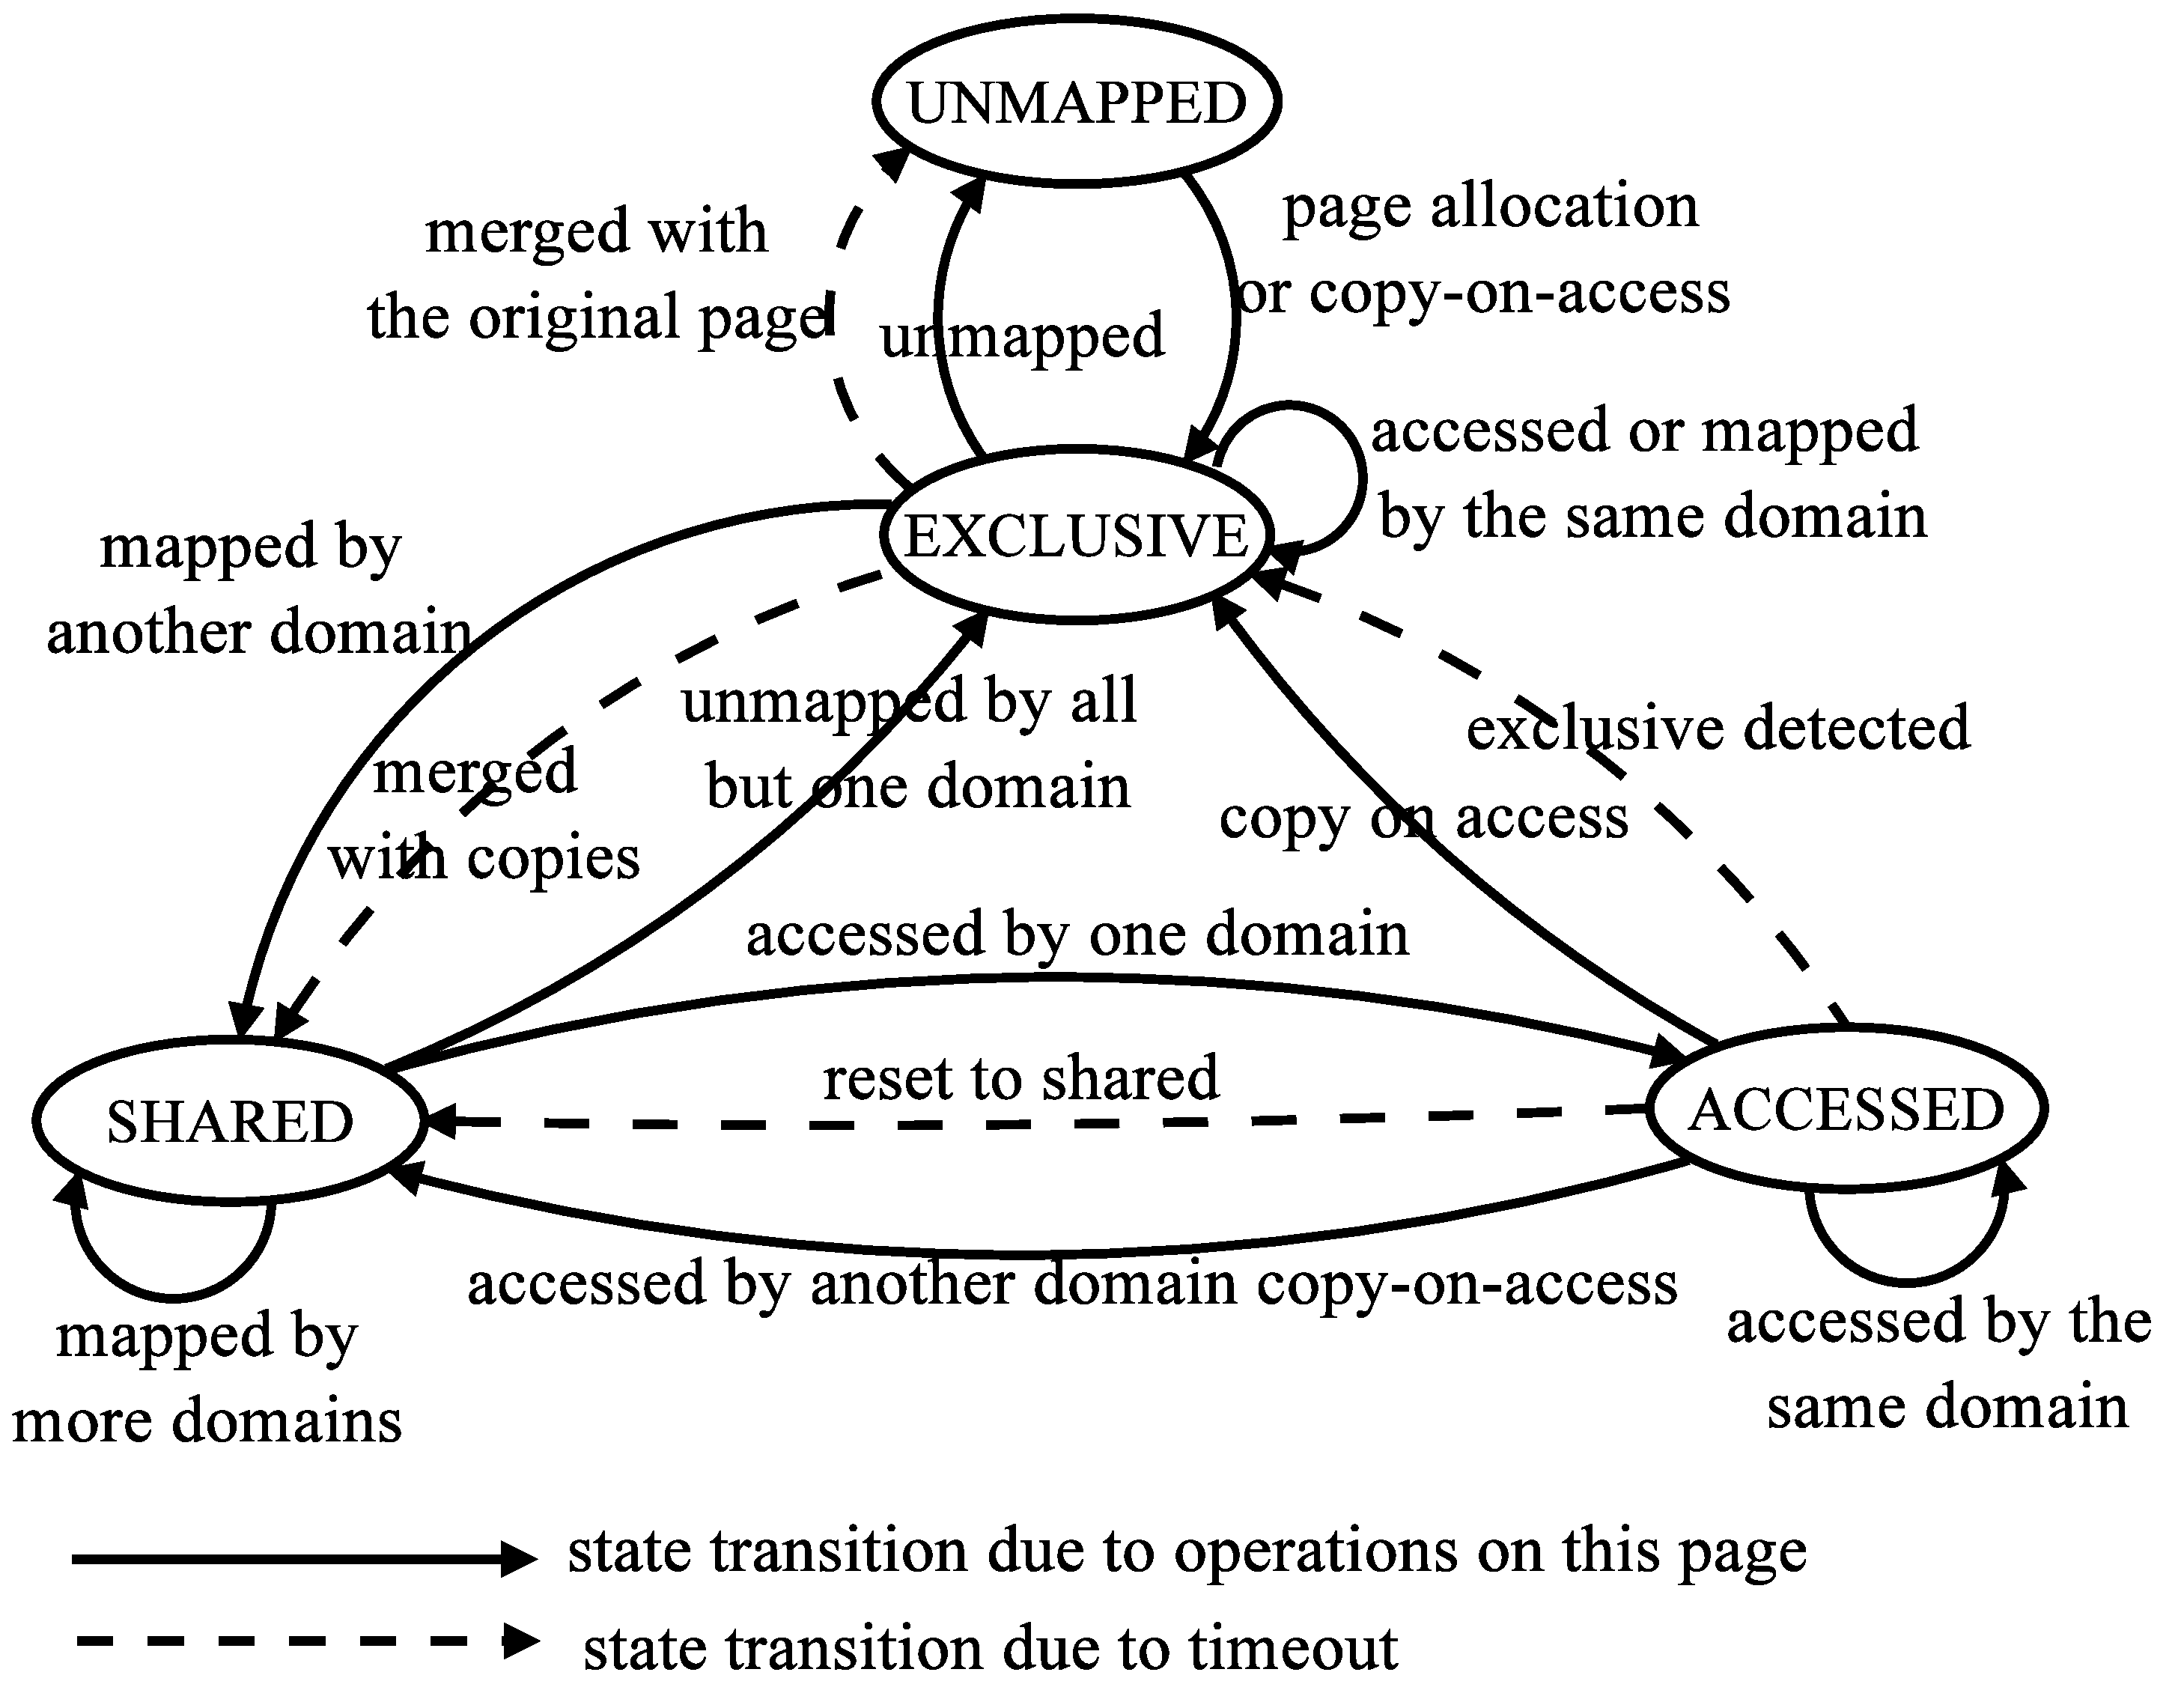
\includegraphics[width=0.7\linewidth]{fig/cachebar/states.eps}
%\resizebox{\linewidth}{!}{\large\input{fig/cachebar/states.eps}}%
\caption{Copy-On-Access State Transition\label{fig:coa}}%
\end{figure}

\cachebar adopts a design that we call \coa, which dynamically controls
the sharing of physical memory pages between security domains. We
designate each physical page as being in exactly one of the following
states: \unmapped, \exclusive, \shared, and \accessed.  An \unmapped
page is a physical page that is not currently in use. An \exclusive
page is a physical page that is currently used by exactly one security
domain, but may be shared by multiple processes in that domain.
A \shared page is a physical page that is shared by multiple security
domains, i.e., mapped by at least one process of each of the sharing
domains, but no process in any domain has accessed this physical page
recently. In contrast, an \accessed page is a previously \shared page
that was recently accessed by a security domain.  The state
transitions are shown in \figref{fig:coa}.

An \unmapped page can transition to the \exclusive state either due to
normal page mapping, or due to copy-on-access when a page is copied
into it.  Unmapping a physical page for any reason (e.g., process
termination, page swapping) will move an \exclusive page back to the
\unmapped state. However, mapping the current \exclusive page by
another security domain will transit it into the \shared state.  If
all but one domain unmaps this page, it will transition back from the
\shared state to the \exclusive state, or \accessed state to the
\exclusive state.  A page in the \shared state may be shared by more
domains and remain in the same state; when any one of the domains
accesses the page, it will transition to the \accessed state. An
\accessed page can stay that way as long only the same security domain
accesses it.  If this page is accessed by another domain, a new
physical page will be allocated to make a copy of this one, and the
current page will transition to either \exclusive or \shared state,
depending on the remaining number of domains mapping this page. The
new page will be assigned state \exclusive.  An \accessed page will be
reset to the \shared state if it is not accessed for \accessedTimeout
seconds. This timeout mechanism ensures that only recently used pages
will remain in the \accessed state, limiting chances for unnecessary
duplication.
Page merging may also be triggered by deduplication services in a
modern \gls{OS} (e.g., \gls{KSM} in Linux).  This effect is reflected by a dashed
line in \figref{fig:coa} from state \exclusive to \shared.  A page
at any of the \textit{mapped} states (i.e., \exclusive, \shared,
\accessed) can transition to \unmapped state for the same reason when
it is a copy of another page (not shown in the figure).

Merging duplicated pages requires some extra bookkeeping. When
a page transitions from \unmapped to \exclusive due to copy-on-access,
the original page is tracked by the new copy so that \cachebar knows
with which page to merge it when deduplicating.  If
the original page is unmapped first, then one of its
copies will be designated as the new ``original''
page, with which other copies will be merged in the future. The interaction between copy-on-access
and existing copy-on-write mechanisms is also implicitly depicted in
\figref{fig:coa}: Upon copy-on-write, the triggering process will first
\textit{unmap} the physical page, possibly inducing a state transition (from
\shared to \exclusive). The state of the newly mapped physical page is
maintained separately.

\subsection{Implementation}
\label{cachebar:sec:coa:impl}

At the core of copy-on-access implementation is the state machine depicted in
\figref{fig:coa}.

\bheading{\unmapped $\Leftrightarrow$ \exclusive
  $\Leftrightarrow$ \shared}
Conventional Linux kernels maintain the relationship between processes
and the physical pages they use.  However, \cachebar also needs to keep
track of the relationship between containers and the physical pages
that each container's processes use.  Therefore, \cachebar incorporates
a new data structure, \pcounterincontainer, which is conceptually a
table used for recording, for each physical page, the number of
processes in each container that have \glspl{PTE} mapped
to this page. 

The \pcounterincontainer data structure is updated and referenced in
multiple places in the kernel.  Specifically, in \cachebar we
instrumented every update of \mapcount, a data field in the
\texttt{page} structure for counting \gls{PTE} mappings, so that every time
the kernel tracks the \gls{PTE} mappings of a physical page,
\pcounterincontainer is updated accordingly. The use of
\pcounterincontainer greatly simplifies maintaining and determining
the state of a physical page: (1) Given a container, access to a
single cell suffices to check whether a physical page is already
mapped in the container. This operation is very commonly used to
decide if a state transition is required when a page is mapped by a
process.  Without \pcounterincontainer, such an operation requires
performing reverse mappings to check the domain of each mapping. (2)
Given a physical page, it takes \containerNmbr accesses to
\pcounterincontainer, where \containerNmbr is the total number of
containers, to tell which containers have mapped to this
page. This operation is commonly used to determine the state of a
physical page.

\bheading{\shared $\Rightarrow$ \accessed}
\begin{figure}[tb]
\centering
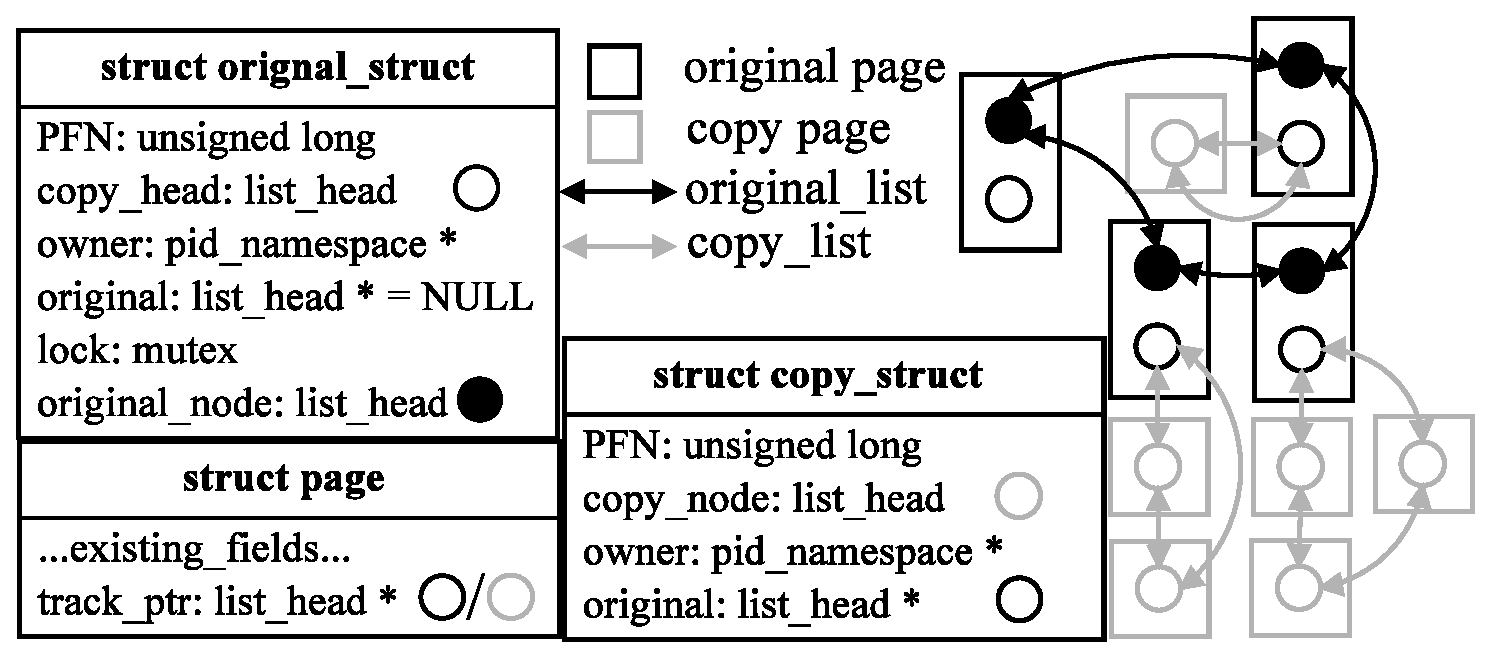
\includegraphics[width=0.7\linewidth]{fig/cachebar/coa_struct.eps}
\caption{Structure of \coa page lists.}
\label{fig:linkedlist}
\end{figure} 
To differentiate \shared and \accessed states, one additional data field,
\owner, is added (see \figref{fig:linkedlist}) to indicate the owner of the page
(a pointer to a \texttt{PID\_namespace} structure). When the page is in the
\shared state, its \owner is \texttt{NULL}; otherwise it points to the
container that last accessed it.

All \gls{PTE}s pointing to a \shared physical page will have a reserved \COA
bit set. Therefore, any access to these virtual pages will induce a
page fault.  When a page fault is triggered, \cachebar checks if the
page is present in physical memory; if so, and if the physical page is
in the \shared state, the \COA bit of the current \gls{PTE} for this page
will be cleared so that additional accesses to this physical page from
the current process will be allowed without page faults.  The physical
page will also transition to the \accessed state.

\bheading{\accessed $\Rightarrow$ \exclusive/\shared}  If the page is
already in the \accessed state when a domain other than the \owner
accesses it, the page fault handler will allocate a new physical page,
copy the content of the original page into the new page, and change
the \gls{PTE}s in the accessing container so that they
point to the new page. Since multiple same-content copies in one
domain burdens both performance and memory but contributes nothing for
security, the fault handler will reuse a copy belonging to that domain
if it exists. After copy-on-access, the original page can either be
\exclusive or \shared.  All copy pages are anonymous-mapped, since
only a single file-mapped page for the same file section is allowed.

A transition from the \accessed state to \shared or \exclusive state
can also be triggered by a timeout mechanism. \cachebar implements a
periodic timer (every $\accessedTimeout = 1\secs$). Upon timer
expiration, all physical pages in the \accessed state that were
not accessed during this \accessedTimeout interval will be reset to
the \shared state by clearing its \owner field, so that pages that are
infrequently accessed are less likely to trigger \coa.  If an
\accessed page is found for which its \pcounterincontainer shows the
number of domains mapped to it is 1, then the daemon instead clears
the \COA bit of all \gls{PTE}s for that page and marks the page \exclusive.

Instead of keeping a list of \accessed pages, \cachebar maintains a
list of pages that are in either \shared or \accessed state, denoted
\originalpagelist (shown in \figref{fig:linkedlist}). Each node in the
list also maintains a list of copies of the page it represents, dubbed
\copypagelist. These lists are attached onto the \texttt{struct page}
through \texttt{track\_ptr}.  Whenever a copy is made from the page
upon \coa, it is inserted into the \copypagelist of the original page.
Whenever a physical page transitions to the \unmapped state, it is
removed from whichever of \originalpagelist or \copypagelist it is
contained in.  In the former case, \cachebar will designate a copy
page of the original page as the new original page and adjust the
lists accordingly.

For security reasons that will be explained in
\secref{cachebar:sec:coa:security}, we further require flushing the entire
memory page out of the cache after transitioning a page from the
\accessed state to the \shared state due to this timeout
mechanism. This page-flushing procedure is implemented by issuing
\texttt{clflush} on each of the memory blocks of any virtual page that
maps to this physical page.

\bheading{State transition upon \clflush} The \clflush instruction is
subject to the same permission checks as a memory load, will trigger
the same page faults,
and will similarly set the ACCESSED bit in the \gls{PTE} of its
argument~\cite{guide2010intel}.  As such, each \Flush via \clflush
triggers the same transitions (e.g., from \shared to \accessed, and
from \accessed to an \exclusive copy) as a \Reload in our
implementation, meaning that this defense is equally effective against
both \flushreload and \flushflush~\cite{gruss:2015:FF} attacks.

\bheading{Page deduplication}  To mitigate the impact of \coa on the
size of memory, \cachebar implements a less frequent timer (every
$\copyTimeout = 10\times\accessedTimeout$ seconds) to periodically
merge the page copies with their original pages. Within the timer
interrupt handler, \originalpagelist and each \copypagelist are
traversed similarly to the ``\accessed $\Rightarrow$ \shared''
transition description above, though the ACCESSED bit in the \gls{PTE}s of
only pages that are in the \exclusive state are checked. If a copy
page has not been accessed since the last such check (i.e., the
ACCESSED bit is unset in all \gls{PTE}s pointing to it), it will be merged
with its original page (the head of the \copypagelist). The ACCESSED
bit in the \gls{PTE}s will be cleared afterwards.

When merging two pages, if the original page is anonymous-mapped, then
the copy page can be merged by simply updating all \gls{PTE}s pointing to
the copy page to instead point to the original page, and then updating
the original page's reverse mappings to include these \gls{PTE}s.  If the
original page is file-mapped, then merging is more
intricate, additionally involving the creation of a new virtual memory
area (\texttt{vma} structure) that maps to the original page's file
position and using this structure to replace the virtual memory area
of the (anonymous) copy page in the relevant task structure.

For security reasons, merging of two pages requires flushing the
original physical page from the \gls{LLC}.  We will elaborate on this point
in \secref{cachebar:sec:coa:security}.

\bheading{Interacting with \gls{KSM}}  
Page deduplication can also be triggered by existing memory
deduplication mechanisms (e.g., \gls{KSM}). To maintain the state of
physical pages, \cachebar instruments every reference to \mapcount
within \gls{KSM} and updates \pcounterincontainer accordingly.
\gls{KSM} is capable of merging more pages than our built-in page
deduplication mechanisms.  However, \cachebar still relies on the built-in page
deduplication mechanisms for several reasons. First, \gls{KSM} can merge only
anonymous-mapped pages, while \cachebar needs to frequently merge an
anonymous-mapped page (a copy) with a file-mapped page (the original). Second,
\gls{KSM} may not be enabled in certain settings, which will lead to ever growing
\copypagelist{s}.  Third, \gls{KSM} must compare page contents byte-by-byte before
merging two pages, whereas \cachebar deduplicates pages on the
same \copypagelist, avoiding the expensive page content comparison.


\section{Cacheability Management}
\label{cachebar:sec:cacheabilityMgmt}

A potentially effective countermeasure to \primeprobe attacks is to
remove the attacker's ability to \Prime and \Probe the whole cache set
and to predict how a victim's demand for that set will be reflected in
the number of evictions from that set.

\subsection{Design}
\label{cachebar:sec:cacheabilityMgmt:design}
\begin{figure}[t]
\centering
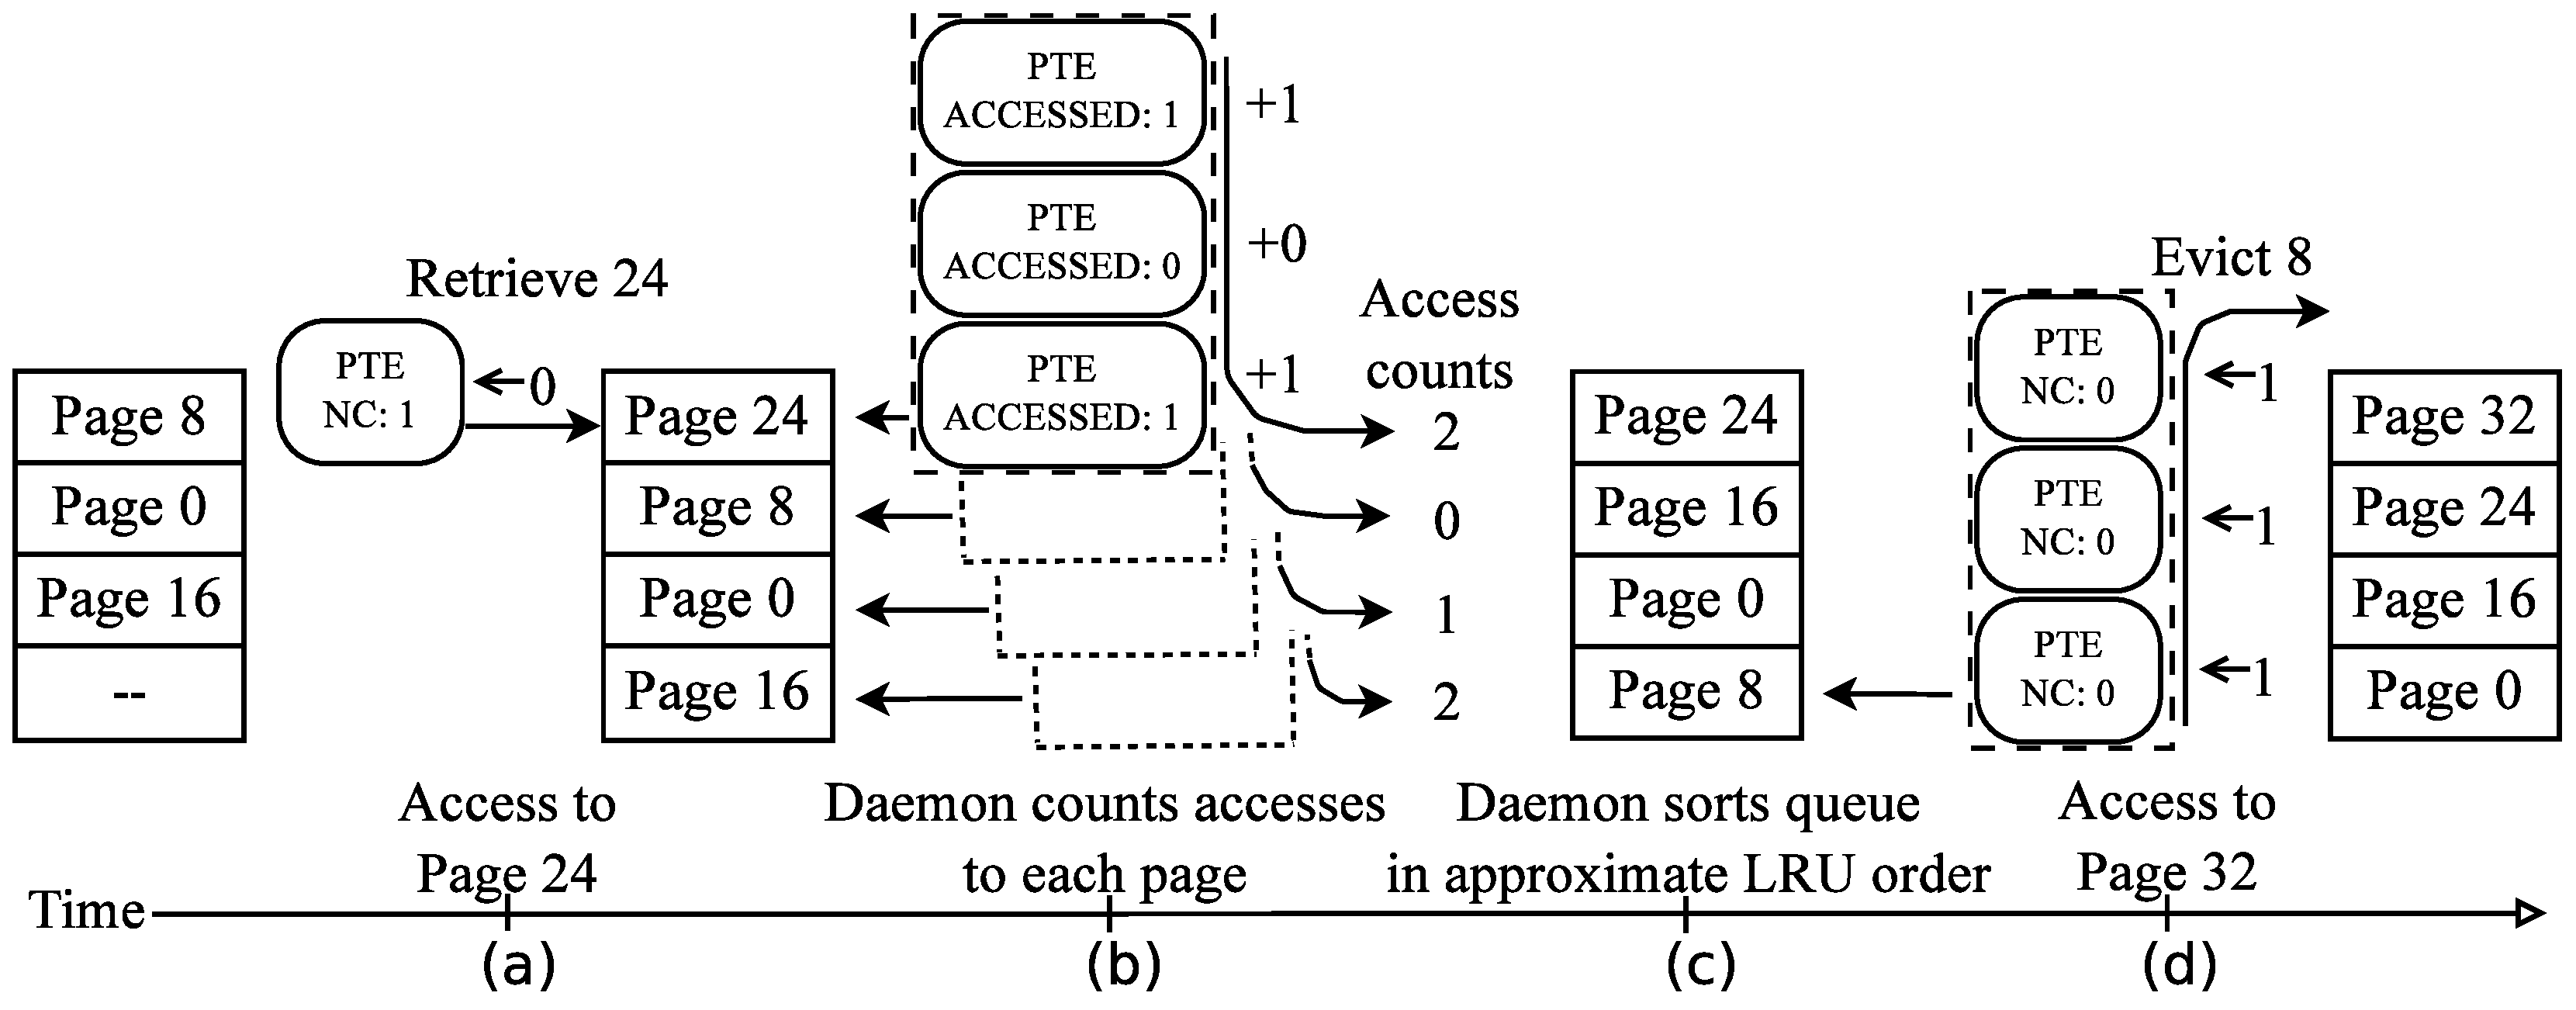
\includegraphics[width=0.85\textwidth]{fig/cachebar/queue-all.eps}
\caption[A \lru for one page color in a domain]{A \lru for one page color in a domain: (a) access to page 24
brings it into the queue and clears NC bit (``$\leftarrow\!0$'') in
the PTE triggering the fault; periodically, (b) a daemon counts
the ACCESSED bits (``$+0$'', ``$+1$'') per page and (c) reorders pages
accordingly; to make room for a new page, (d) NC bits in PTE
pointing to the least recently used page are set, and the page is
removed from the queue.}
\label{fig:queues:all}
\vspace{-0.1in}
\end{figure}
Suppose a \cacheLineNmbr-way set associative \gls{LLC}, so that each
cache set has \cacheLineNmbr lines.  Let \evictedNmbr be the number of
cache lines in one set that the attacker observes having been evicted
in a \primeprobe interval (i.e., $\evictedNmbr \in \AOOKeys{}$).  The
\primeprobe attack is effective today because \evictedNmbr is
typically a good indicator of the demand \victimDemand that the victim
security domain had for memory that mapped to that cache set during
the \primeprobe interval (i.e., $\victimDemand\in \SecKeys{}$).  In
particular, if the attacker \Prime{s} and \Probe{s} all \cacheLineNmbr
lines, then it can often observe the victim's demand \victimDemand
exactly, unless $\victimDemand > \cacheLineNmbr$ (in which case the
attacker learns at least $\victimDemand \ge \cacheLineNmbr$).

Here we propose to periodically and
probabilistically reconfigure the budget
\linesPerContainer{\containerIdx} of lines per cache set that the
security domain \containerIdx can occupy.  After such a
reconfiguration, the attacker's view of the victim's demand
\victimDemand is clouded by the following three effects.  First, if
the attacker is allotted a budget $\linesPerContainer{\attackerLabel}
< \cacheLineNmbr$, then the attacker will be unable to observe any
evictions at all (i.e., $\evictedNmbr=0$) if $\victimDemand <
\cacheLineNmbr-\linesPerContainer{\attackerLabel}$.\footnote{This
  statement assumes a LRU replacement policy and that
  the victim is the only security domain that runs in the \primeprobe
  interval.  If it was not the only security domain to run, then the ambiguity of 
  the observable evictions will additionally cause difficulties for
  the attacker.}  Second, if the victim is given allotment
\linesPerContainer{\victimLabel}, then any two victim demands
\victimDemand, \victimDemandAlt satisfying $\victimDemand >
\victimDemandAlt \ge \linesPerContainer{\victimLabel}$ will be
indistinguishable to the attacker.  Third, the probabilistic
assignment of \linesPerContainer{\victimLabel} results in extra
ambiguity for the attacker, since \evictedNmbr evictions might reflect
the demand \victimDemand or the budget
\linesPerContainer{\victimLabel}, since $\evictedNmbr \le
\min\{\victimDemand,\linesPerContainer{\victimLabel}\}$ (if all
\evictedNmbr evictions are caused by the victim).

To enforce the budget \linesPerContainer{\containerIdx} of lines that
security domain \containerIdx can use in a given cache set, \cachebar
maintains for each cache set a queue per security domain that records
which memory blocks are presently cacheable in this set by processes
in this domain.  Each element in the queue indicates a memory block
that maps to this cache set; only blocks listed in the queue can be
cached in that set.  The queue is maintained with a least recently
used (LRU) replacement algorithm. That is, whenever a new memory block
is accessed, it will replace the memory block in the corresponding
queue that is the least recently used.

\subsection{Dynamic budget \linesPerContainer{\containerIdx} of
cache lines}
\label{cachebar:sec:cacheabilityMgmt:security}
\if0
While the budget \linesPerContainer{\containerIdx} is in effect, each
access to a memory block that maps to this cache set, beyond the
in-queue \linesPerContainer{\containerIdx} memory blocks, will incur a
page fault (because they are all in different pages).  Because the
page-fault processing time will overwhelm the timing granularity of
modern \primeprobe attacks by an order of magnitude, the attacker
\containerIdx realistically needs to restrict himself to accessing
\linesPerContainer{\containerIdx} pages in his \Probe phase and hence
to occupying \linesPerContainer{\containerIdx} lines in that cache
set. The security of this design hinges critically on how each
\linesPerContainer{\containerIdx} is set by the daemon.  When
\linesPerContainer{\containerIdx} is reset, it is drawn from a
distribution.  In the remainder of this section we present how this
distribution is determined.
\fi

Suppose there are (at most) \attackerNmbr domains on a host that are
owned by the attacker---which might be all  domains on the host except
the victim---and let \cacheLineNmbr be the number of cache lines per
\gls{LLC} set. Below we consider domain $0$ to be the ``victim''
domain being subjected to \primeprobe attacks by the ``attacker''
domains $1, \ldots, \attackerNmbr$.  Of course, the attacker domains
make use of all $\sum_{\containerIdx=1}^{\attackerNmbr}
\linesPerContainer{\containerIdx}$ cache lines available to them for
conducting their \primeprobe attacks.

Periodically, \cachebar draws a new value
\linesPerContainer{\containerIdx} for each security domain
\containerIdx.  This drawing is memoryless and independent of the
draws for other security domains.  Let
\linesPerContainerRV{\containerIdx} denote the random variable
distributed according to how \linesPerContainer{\containerIdx} is
determined.  The random variables that we presume can be observed by
the attacker domains include $\linesPerContainerRV{1}, \ldots,
\linesPerContainerRV{\attackerNmbr}$; let $\attackerLineNmbrRV{}\!=
\!\min\left\{\cacheLineNmbr, \sum_{\containerIdx=1}^{\attackerNmbr}
\linesPerContainerRV{\containerIdx}\right\}$ denote the number of
cache lines allocated to the attacker domains.  We also presume the
attacker can accurately measure the number \evictedNmbrRV of its cache
lines that are evicted during the victim's execution.

Let \prob{\victimDemand}{\genericEvent} denote the probability of
event \genericEvent in an execution period during which the victim's
cache usage would populate \victimDemand lines (of this color) if it
were allowed to use all \cacheLineNmbr lines, i.e., if
$\linesPerContainer{0} = \cacheLineNmbr$.  We (the defender) would
like to distribute $\linesPerContainerRV{0}, \ldots,
\linesPerContainerRV{\attackerNmbr}$
so as to minimize the statistical distance between eviction
distributions observable by the attacker for different victim demands
\victimDemand, \victimDemandAlt, i.e., to minimize
\begin{align}
\sum_{0 \le \victimDemand < \victimDemandAlt \le \cacheLineNmbr} \sum_{\evictedNmbr} |\prob{\victimDemand}{\evictedNmbrRV = \evictedNmbr} - \prob{\victimDemandAlt}{\evictedNmbrRV = \evictedNmbr}|
\label{eqn:securityGoal}
\end{align}

We begin by deriving an expression
for \prob{\victimDemand}{\evictedNmbrRV = \evictedNmbr}.  Below we
make the conservative assumption that all evictions are caused by the
victim's behavior; in reality, caches are far noisier.  We first
consider the case $\evictedNmbr=0$, i.e., that the attacker domains
observe no evictions.
\begin{align*}
\cprob{\Big}{\victimDemand}{\evictedNmbrRV =
0}{\linesPerContainerRV{0} = \linesPerContainer{0}
\wedge~\attackerLineNmbrRV =
\attackerLineNmbr}
& \!=\! \left\{\begin{array}{@{\extracolsep{-0.4em}}ll}
1 & \mbox{if $\cacheLineNmbr \ge \attackerLineNmbr + \min\{\linesPerContainer{0}, \victimDemand\}$} \\
0 & \mbox{otherwise}
\end{array}\right.
\end{align*}
``$\min\{\linesPerContainer{0}, \victimDemand\}$'' is used above
because any victim demand for memory blocks that map to this cache set
beyond \linesPerContainer{0} will back-fill the cache lines invalidated
when \cachebar flushes other blocks from the victim's cacheability
queue, rather than evicting others.  Since \linesPerContainerRV{0} and
\attackerLineNmbrRV are independent,
\begin{align}
\prob{\victimDemand}{\evictedNmbrRV = 0}
& = \sum_{\linesPerContainer{0}=0}^{\victimDemand}
\sum_{\attackerLineNmbr=0}^{\cacheLineNmbr-\linesPerContainer{0}}
\prob{}{\linesPerContainerRV{0} = \linesPerContainer{0}} \cdot
\prob{}{\attackerLineNmbrRV = \attackerLineNmbr}
 + \sum_{\linesPerContainer{0}=\victimDemand+1}^{\cacheLineNmbr} \sum_{\attackerLineNmbr=0}^{\cacheLineNmbr-\victimDemand} \prob{}{\linesPerContainerRV{0} = \linesPerContainer{0}} \cdot \prob{}{\attackerLineNmbrRV = \attackerLineNmbr} \label{eqn:zeroEvictions}
\end{align}
Note that we have dropped the ``\victimDemand'' subscripts from the
probabilities on the right, since \linesPerContainerRV{0}
and \attackerLineNmbrRV are distributed independently
of \victimDemand.  And, since
$\linesPerContainerRV{1},\ldots,\linesPerContainerRV{\attackerNmbr}$
are independent,
\begin{align}
\prob{}{\attackerLineNmbrRV\!=\!\attackerLineNmbr} = \!\begin{cases}
\displaystyle
\sum_{ \linesPerContainer{1}\!+\ldots+\!\linesPerContainer{\attackerNmbr}=\attackerLineNmbr} \prod_{\containerIdx=1}^{\attackerNmbr} \prob{}{\linesPerContainerRV{\containerIdx} = \linesPerContainer{\containerIdx}} & \mbox{if $\attackerLineNmbr\!<\!\cacheLineNmbr$}\\
\displaystyle
\sum_{\linesPerContainer{1}\!+\ldots+\!\linesPerContainer{\attackerNmbr}\ge\cacheLineNmbr} \prod_{\containerIdx=1}^{\attackerNmbr} \prob{}{\linesPerContainerRV{\containerIdx} = \linesPerContainer{\containerIdx}} & \mbox{if $\attackerLineNmbr\!=\!\cacheLineNmbr$}
\end{cases}
\label{eqn:attackerLineNmbr}
\end{align}

Similarly, for $\evictedNmbr \ge 1$, 
\begin{align*}
\cprob{\Big}{\victimDemand}{\evictedNmbrRV=\evictedNmbr}{\linesPerContainerRV{0} = \linesPerContainer{0} \wedge\attackerLineNmbrRV = \attackerLineNmbr}
& = \left\{\begin{array}{ll}
1 & \mbox{if $\evictedNmbr\! +\!\cacheLineNmbr = \attackerLineNmbr\! + \!\min\{\linesPerContainer{0}, \victimDemand\}$} \\
0 & \mbox{otherwise}
\end{array}\right.
\end{align*}
and so for $\evictedNmbr \ge 1$,
\begin{align}
\prob{\victimDemand}{\evictedNmbrRV = \evictedNmbr}
& = \sum_{\linesPerContainer{0}=0}^{\victimDemand} \prob{}{\linesPerContainerRV{0} = \linesPerContainer{0}} \cdot \prob{}{\attackerLineNmbrRV = \evictedNmbr\! +\! \cacheLineNmbr \!-\! \linesPerContainer{0}} 
+\sum_{\linesPerContainer{0}=\victimDemand+1}^{\cacheLineNmbr} \hspace{-0.53em}\prob{}{\linesPerContainerRV{0} = \linesPerContainer{0}} \cdot \prob{}{\attackerLineNmbrRV = \evictedNmbr\! +\! \cacheLineNmbr \!-\! \victimDemand}
\label{eqn:moreThanZeroEvictions}
\end{align}

From here, we proceed to solve for the best distribution for
$\linesPerContainerRV{0}, \ldots, \linesPerContainerRV{\attackerNmbr}$
to minimize \eqnref{eqn:securityGoal} subject to
constraints \eqnsref{eqn:zeroEvictions}{eqn:moreThanZeroEvictions}.
That is, we specify
those constraints, along with
\begin{align}
\forall \containerIdx, \containerIdxAlt, \linesPerContainer{}:~ &
\prob{}{\linesPerContainerRV{\containerIdx} = \linesPerContainer{}} = \prob{}{\linesPerContainerRV{\containerIdxAlt} = \linesPerContainer{}} \label{eqn:allDistsSame}\\
\forall \containerIdx:~ &
\sum_{\linesPerContainer{\containerIdx} = 0}^{\cacheLineNmbr} \prob{}{\linesPerContainerRV{\containerIdx} = \linesPerContainer{\containerIdx}} = 1 \\
\forall \containerIdx, \linesPerContainer{\containerIdx}:~ &
\prob{}{\linesPerContainerRV{\containerIdx} = \linesPerContainer{\containerIdx}} \ge 0 \label{eqn:nonnegProbs}
\end{align}
and then solve for each \prob{}{\linesPerContainerRV{\containerIdx}
= \linesPerContainer{\containerIdx}} to
minimize \eqnref{eqn:securityGoal}.

Unfortunately, solving to minimize \eqnref{eqn:securityGoal} alone
simply results in a distribution that results in no use of the cache
at all (e.g., $\prob{}{\linesPerContainerRV{\containerIdx}=0} = 1$ for
each \containerIdx).  As such, we need to rule out such degenerate
and ``unfair'' cases:
\begin{align}
\forall \containerIdx:~ &
\prob{}{\linesPerContainerRV{\containerIdx}
        < \cacheLineNmbr/(\attackerNmbr+1)} = 0
\label{eqn:fairness}
\end{align}
Also, to encourage cache usage, we counterbalance
\eqnref{eqn:securityGoal} with a second goal that
values greater use of the cache.  We express this goal as minimizing
the earth mover's distance~\cite{elizaveta2001emd} from
the distribution that assigns
$\prob{}{\linesPerContainerRV{\containerIdx} = \cacheLineNmbr} = 1$,
i.e.,
\begin{align}
\sum_{\linesPerContainer{}=0}^{\cacheLineNmbr} (\cacheLineNmbr-\linesPerContainer{})
\cdot \prob{}{\linesPerContainerRV{0} = \linesPerContainer{}}
\label{eqn:performanceGoal}
\end{align}

As such, the final optimization problem seeks to balance
\eqnref{eqn:securityGoal} and \eqnref{eqn:performanceGoal}.  Let
constant \maxSecValue denote the maximum (i.e., worst) possible value
of \eqnref{eqn:securityGoal} (i.e., when
$\prob{}{\linesPerContainerRV{\containerIdx}=\cacheLineNmbr} = 1$ for
each \containerIdx) and \maxPerfValue denote the maximum (i.e., worst)
possible value of \eqnref{eqn:performanceGoal} (i.e., when
$\prob{}{\linesPerContainerRV{\containerIdx}=0} = 1$ for
each \containerIdx).  Then, given a parameter \balanceSlack, $0
< \balanceSlack < 1$, our optimization computes
distributions
for $\linesPerContainerRV{0}, \ldots, \linesPerContainerRV{\attackerNmbr}$
so as to minimize \balanceValue subject to
\vspace{-5pt}
\begin{align*}
\balanceValue & = \frac{1}{\maxSecValue} \left(\sum_{0 \le \victimDemand < \victimDemandAlt \le \cacheLineNmbr} \sum_{\evictedNmbr} |\prob{\victimDemand}{\evictedNmbrRV = \evictedNmbr} - \prob{\victimDemandAlt}{\evictedNmbrRV = \evictedNmbr}|\right) \\
\balanceValue & \ge \frac{1}{\maxPerfValue(1+\balanceSlack)} \left(\sum_{\linesPerContainer{}=0}^{\cacheLineNmbr} (\cacheLineNmbr-\linesPerContainer{})
\cdot \prob{}{\linesPerContainerRV{0} = \linesPerContainer{}}\right)
\end{align*}
and constraints \eqnsref{eqn:zeroEvictions}{eqn:fairness}.

The evaluation in \secref{cachebar:sec:eval:security:primeprobe}
empirically characterizes the security that result from setting
$\balanceSlack = 0.01$ the default setting in \cachebar.  

\subsection{Implementation}
\label{cachebar:sec:cacheabilityMgmt:impl}

Implementation of \lru{s} is processor micro-architecture dependent.
Here we focus our attention on Intel x86 processors, which appears to
be more vulnerable to \primeprobe attacks due to their inclusive
last-level cache~\cite{liu2015practical}.  As x86 architectures only
support memory management at the page granularity (e.g., by
manipulating the \gls{PTE}s to cause page faults), \cachebar controls the
cacheability of memory blocks at page granularity.  \cachebar uses
reserved bits in each \gls{PTE} to manage the cacheability of, and to track
accesses to, the physical page to which it points, since a reserved
bit set in a \gls{PTE} induces a page fault upon access to the associated
virtual page, for which the backing physical page cannot be retrieved
or cached (if it is not already) before the bit is
cleared~\cite{guide2010intel,raikin2014tracking}.  We hence use the
term \textit{domain-cacheable} to refer to a physical page that is
``cacheable'' in the view of all processes in a particular security
domain, which is implemented by modifying all relevant \gls{PTE}s (to have
no reserved bits set) in the processes of that security domain. By
definition, a physical page that is domain-cacheable to one container
may not necessarily be domain-cacheable to another.

To ensure that no more than \linesPerContainer{\containerIdx} memory
blocks from all processes in container \containerIdx can occupy lines
in a given cache set, \cachebar ensures that no more than
\linesPerContainer{\containerIdx} of those processes' physical
memory pages, of which contents can be stored in that cache set, are
domain-cacheable at any point in time. Physical memory pages of which
contents can be stored in the same cache set are said to be of the
same \textit{color}, and so to implement this property, \cachebar
maintains, per container and per color (rather than per cache set),
one \lru, each element of which is a physical memory page that is
domain-cacheable in this container.  Since the memory blocks in each
physical page map to different cache sets, limiting the
domain-cacheable pages of a color to \linesPerContainer{\containerIdx}
also limits the number of cache lines that blocks from these pages can
occupy in the same cache set to \linesPerContainer{\containerIdx}.

To implement a non-domain-cacheable memory, \cachebar uses one
reserved bit, which we denote by \LRU, in all \gls{PTE}s within the domain
mapped to that physical page.  As such, accesses to any of these
virtual pages will be trapped into the kernel and handled by the page
fault handler. Upon detecting page faults of this type, the page fault
handler will move the accessed physical page into the corresponding
\lru, clear the \LRU bit in the current \gls{PTE}\footnote{We avoid the
overhead of traversing all \gls{PTE}s in the container that map to this
physical page. Access to those virtual pages will trigger page faults
to make these updates without altering the \lru.}, and remove a least
recently used physical page from the \lru and set the \LRU bits in
this domain's \gls{PTE}s mapped to that page.  A physical page removed from
the \lru will be flushed out of the cache using \clflush instructions
on all of its memory blocks to ensure that no residue remains in the
cache. \cachebar will flush the translation lookaside buffers (TLB) of
all processors to ensure the correctness of page cacheabilities every
time \gls{PTE}s are altered. In this way, \cachebar limits the number of
domain-cacheable pages of a single color at any time to
\linesPerContainer{\containerIdx}.

To maintain the LRU property of the \lru, a daemon periodically
re-sorts the queue in descending order of recent access count.
Specifically, the daemon traverses the domain's
\glspl{PTE} mapped to the \ppage within that domain's queue and counts the number having their ACCESSED bit set, after which
it clears these ACCESSED bits.  It then orders the physical pages in
the \lru by this count (see \figref{fig:queues:all}).  In our present
implementation, this daemon is the same daemon that resets pages from
the \accessed state to \shared state (see \secref{cachebar:sec:coa}), which
already checks and resets the ACCESSED bits in copies' \gls{PTE}s.  Again, this
daemon runs every $\accessedTimeout = 1\secs$ seconds in our
implementation.  This daemon also performs the task of resetting
\linesPerContainer{\containerIdx} for each security domain
\containerIdx, each time it runs.

\begin{figure}[bt]
	\centering
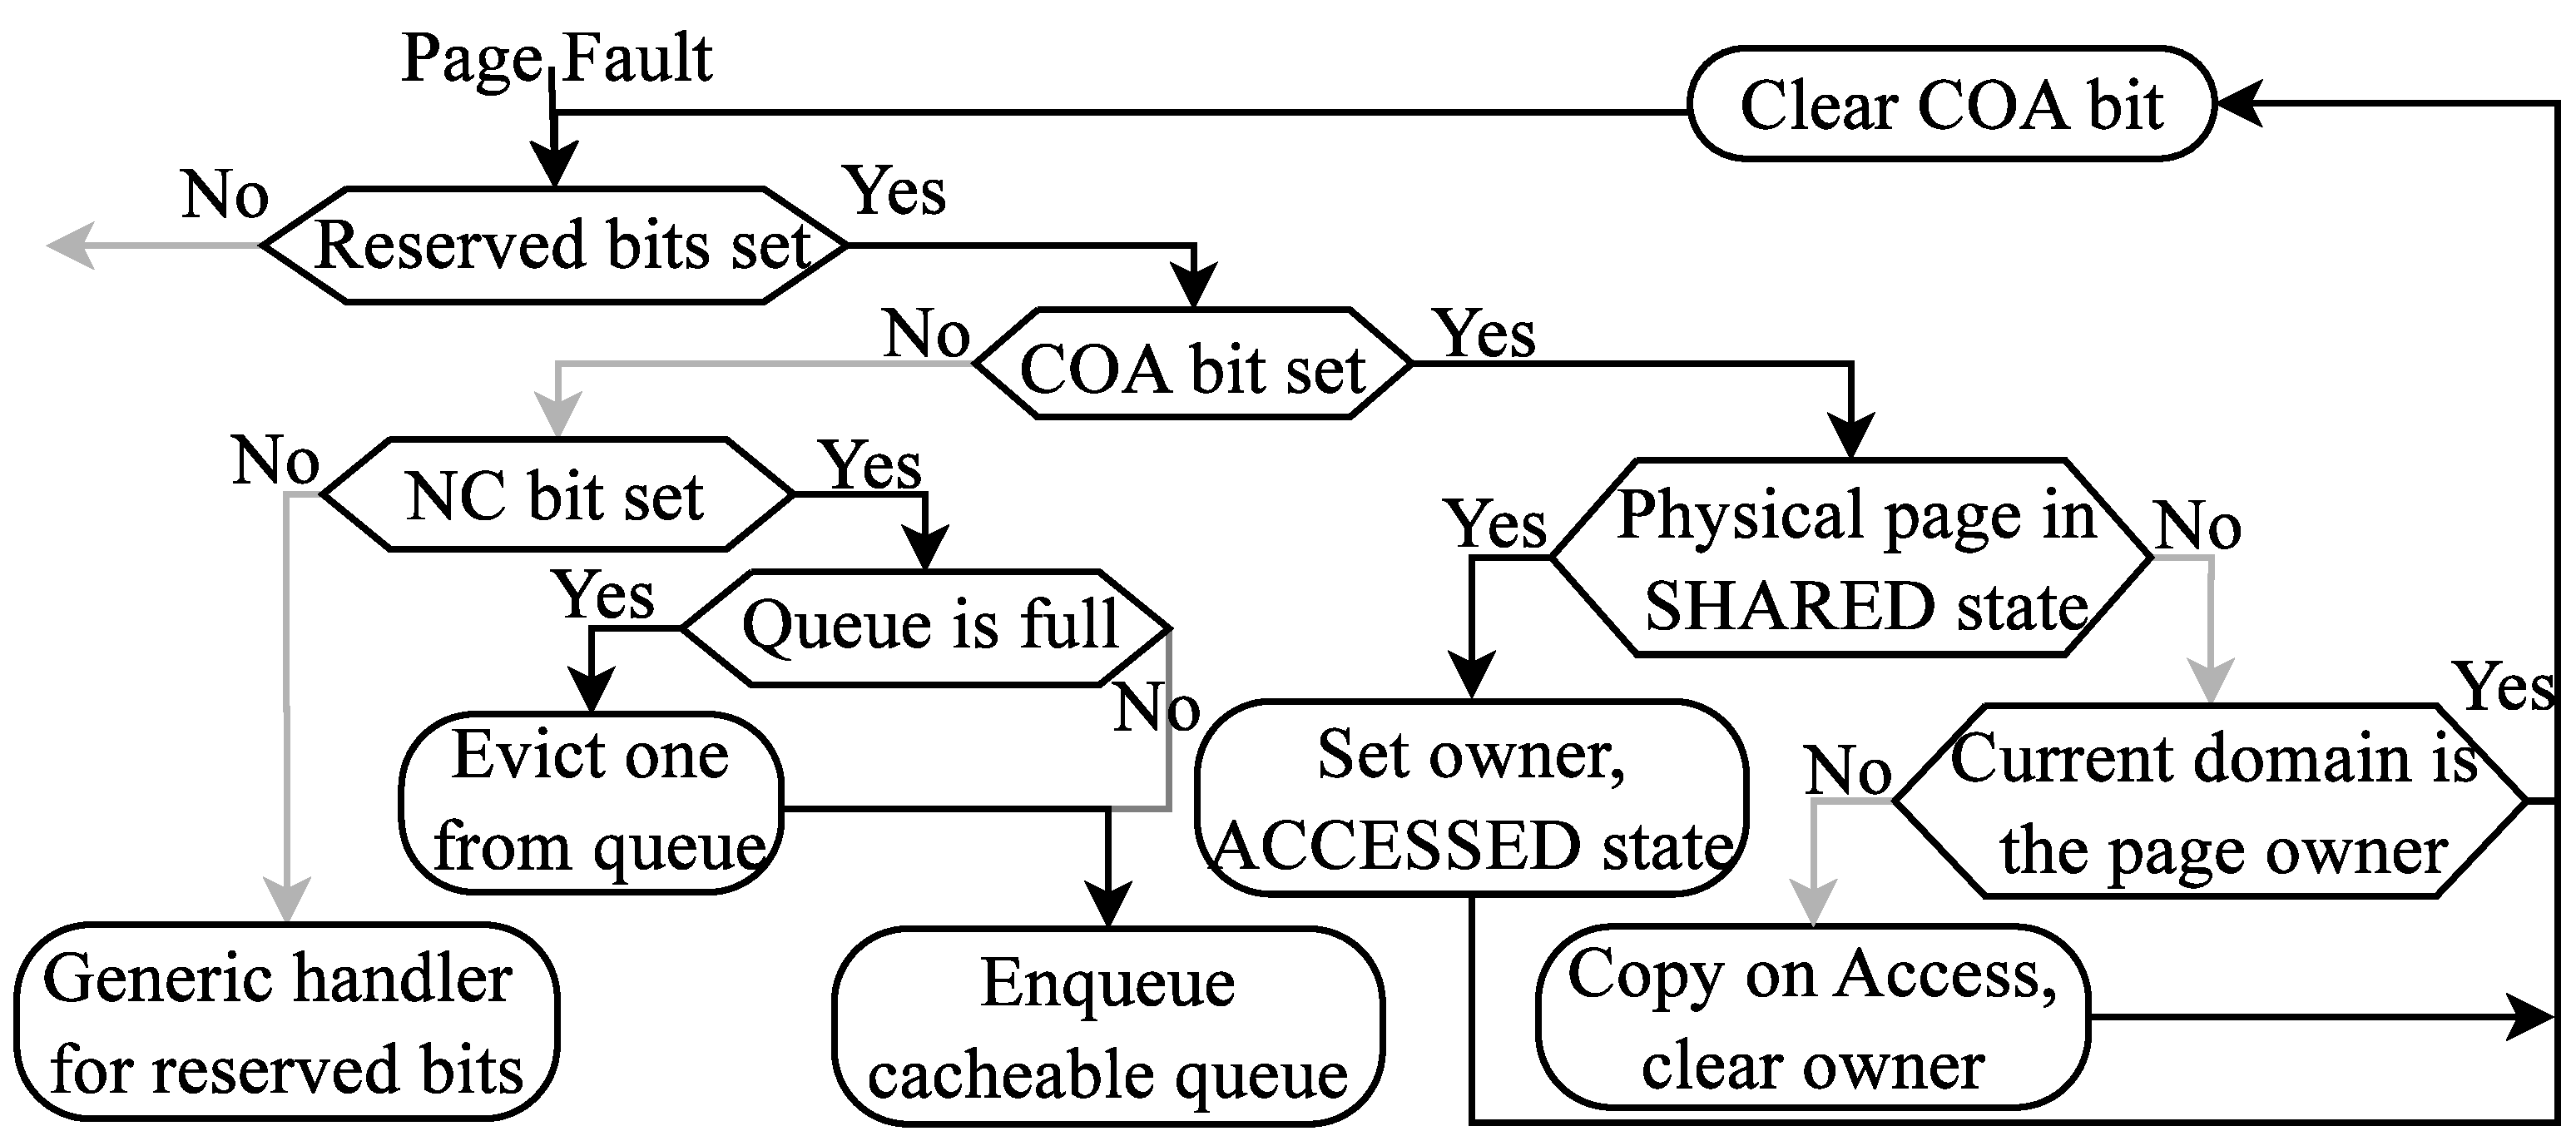
\includegraphics[width=0.9\linewidth]{fig/cachebar/page_fault.eps}
\caption{Page fault handler for \cachebar.\label{fig:fault}}
 \vspace{-0.1in}
\end{figure}

\bheading{Interacting with copy-on-access} The \lru{s} work closely
with the copy-on-access mechanisms. In particular, as both the \COA
and \LRU bits may trigger a page fault upon page accesses, the page
handler logic must incorporate both (see \figref{fig:fault}). First, a page
fault is handled as normal unless it is due to one of the reserved
bits set in the \gls{PTE}. As \cachebar is the only source of reserved bits,
it takes over page fault handling from this point. \cachebar first
checks the \COA bit in the \gls{PTE}. If it is set, the corresponding
physical page is either \shared, in which case it will be transitioned
to \accessed, or \accessed, in which case it will be copied and transitioned to either \shared or \exclusive.  \cachebar
then clears the \COA bit and, if no other reserved bits are set, the
fault handler returns.  Otherwise, if the \LRU bit is set, the
associated physical page is not in the \lru for its domain, and so
\cachebar enqueues the page and, if the queue is full, removes the
least-recently-used page from the queue.  If the \LRU bit is clear,
this page fault is caused by unknown reasons and \cachebar turns
control over to the generic handler for reserved bits.

\section{Security Evaluation}
\label{cachebar:sec:eval:security}
In this section, We empirically evaluated the effectiveness of \cachebar in
defending against both \flushreload and \primeprobe attacks.

Our testbed is a rack mounted DELL server equipped with two 2.67\gigahertz Intel Xeon
5550 processors. Each processor contains 4 physical cores (hyperthreading
disabled) sharing an 8\megabytes last-level cache (L3). Each core has a
32\kilobytes L1 data and instruction cache and a 256\kilobytes L2 unified cache.  The
rack server is equipped with 128\gigabytes DRAM and 1000\megabytes NIC connected to a
1000\megabytes ethernet.

We implemented \cachebar as a kernel extension for Linux kernel
3.13.11.6 that runs Ubuntu 14.04 server edition. We set up containers
using \docker 1.7.1.
\subsection{\flushreload attacks}
\label{cachebar:sec:eval:security:flushreload}
We
constructed a \flushreload covert channel between sender and
receiver processes, which were isolated in different containers. Both
the sender and receiver were linked to a shared library,
\texttt{libcrypto.so.1.0.0}, and were pinned to run on different cores
of the same socket, thus sharing the same last-level cache. The sender
ran in a loop, repeatedly accessing one memory location (the beginning
address of function \texttt{AES\_decrypt()}). The receiver executed
\flushreload attacks on the same memory address, by first \Flush{ing}
the memory block out of the shared \gls{LLC} with an \clflush instruction
and then \Reload{ing} the block by accessing it directly
while measuring the access latency. The interval between \Flush and
\Reload was set to 2500 \cycles. The experiment was run for 500,000
\flushreload trials.  We then repeated this experiment with the sender
accessing an unshared address, to form a baseline.

\begin{figure}[t]
\centering
\begin{subfigure}[b]{0.49\textwidth}
\includegraphics[width=0.95\linewidth]{fig/cachebar/eval/flushreload.eps}
\caption{\cachebar disabled}
\label{fig:flushreload_covert:linux}
\end{subfigure}
\begin{subfigure}[b]{0.49\textwidth}
\includegraphics[width=0.95\linewidth]{fig/cachebar/eval/flushreload-w.eps}
\caption{\cachebar enabled}
\label{fig:flushreload_covert:cachebar}
\end{subfigure}
\vspace{-0.1in}\caption{\Reload timings in \flushreload attacks on a
  shared address vs.\ on an unshared address}
\label{fig:flushreload_covert}
\end{figure}

\figref{fig:flushreload_covert:linux} shows the results of this
experiment, when run over unmodified Linux.
The three horizontal lines forming the ``box'' in each boxplot
represents the first, second (median), and third quartiles of the
\flushreload measurements; whiskers extend to cover all points that
lie within $1.5\times$ the interquartile range.  As can be seen in
this figure, the times observed by the receiver to \Reload the shared
address were clearly separable from the times to \Reload the unshared
address, over unmodified Linux.  With \cachebar enabled, however, these
measurements are no longer separable (\figref{fig:flushreload_covert:cachebar}).
Certain corner cases are not represented in
\figref{fig:flushreload_covert}.  For example, we found it extremely
difficult to conduct experiments to capture the corner cases where
\Flush and \Reload takes place right before and after physical page
mergers, as described in \secref{cachebar:sec:coa:security}. As such, we rely
on our manual inspection of the implementation in these cases to check
correctness and argue these corner cases are very difficult to exploit
in practice.

\subsubsection{Model Checking Noninterference}

%Model checking notation
\newcommand{\mcPagesArray}{\texttt{pages}\xspace}
\newcommand{\mcPages}[1]{\texttt{pages[{#1}]}\xspace}
\newcommand{\mcVirt}{\texttt{virt}\xspace}
\newcommand{\mcState}{\texttt{state}\xspace}
\newcommand{\mcOwner}{\texttt{owner}\xspace}
\newcommand{\mcNoOwner}{\texttt{none}\xspace}

\label{cachebar:sec:coa:security}
Copy-on-access is intuitively secure by design, as no two security
domains may access the same physical page at the same time, rendering
a general \Flush+\Reload attack seemingly impossible, as demonstrated in
previous section.  To show security formally, we subjected our design
to model checking in order to ensure that \coa is secure against
\flushreload attacks at every execution point.  Model checking is an
approach to formally verify a specification of a finite-state
concurrent system expressed as temporal logic formulas, by traversing
the finite-state machine defined by the model.  In our study, we used
the \spin model checker, which offers efficient ways to model
concurrent systems and verify temporal logic specifications.

\bheading{System modeling}
We model a physical page in \figref{fig:coa} using a byte
variable in the \textsc{Promela} programming language, and two
physical pages as an array of two such variables, named
\texttt{pages}.  We model two security domains (e.g., containers), an
attacker domain and a victim domain, as two processes in
\textsc{Promela}.  Each process maps a virtual page, \mcVirt, to one
of the physical pages. The virtual page is modeled as an index to the
\mcPagesArray{} array; initially \mcVirt for both the attacker and the
victim point to the first physical page (i.e., \mcVirt is $0$).  The
victim process repeatedly sets \mcPages{\mcVirt} to $1$, simulating a
memory access that brings \mcPages{\mcVirt} into cache.  The attacker
process \Flush{es} the virtual page by assigning $0$ to
\mcPages{\mcVirt} and \Reload{s} it by assigning $1$ to
\mcPages{\mcVirt} after testing if it already equals to $1$.  Both the
\Flush and \Reload operations are modeled as atomic to
simplify the state exploration.

We track the state and owner of the first physical page using another
two variables, \mcState and \mcOwner.  The first page is initially in
the \shared state (\mcState is \shared), and state transitions in
\figref{fig:coa} are implemented by each process when they access
the memory.  For example, the \Reload code snippet run by the attacker
is shown in \figref{fig:codesnippet}.  If the attacker has access to
the shared page (\lineref{lst:codesnippet:sharedPage}), versus an
exclusive copy (\lineref{lst:codesnippet:exclusivePage}), then it
simulates an access to the page, which either moves the state of the
page to \accessed (\lineref{lst:codesnippet:toAccessed}) if the state
was \shared (\lineref{lst:codesnippet:testShared}) or to \exclusive
(\lineref{lst:codesnippet:toExclusive}) after making a copy
(\lineref{lst:codesnippet:coa}) if the state was already \accessed and
not owned by the attacker (\lineref{lst:codesnippet:testAccessed}).
Leakage is detected if \mcPages{\mcVirt} is $1$ prior to the
attacker setting it as such (\lineref{lst:codesnippet:retrieve}), which
the attacker tests in \lineref{lst:codesnippet:leakage}.

\begin{figure}[h]
\vspace{-0.1in}
\lstset{language=Promela,
backgroundcolor=\color{white},
commentstyle=\scriptsize\ttfamily,
keepspaces=true,
basicstyle=\scriptsize\ttfamily,
keywordstyle=\scriptsize\bf,
numberstyle=\tiny\color{black},
rulecolor=\color{black},
morekeywords={atomic,if}
numbersep=8pt,
xleftmargin=2em,
breaklines=true, showstringspaces=false,
escapeinside={(*}{*)},
escapechar=|,
numberblanklines=false,
frame=lines, numbers=left, stepnumber=1} 
\centering
\begin{minipage}{0.7\linewidth}
\begin{lstlisting}
atomic {
if
::(virt == 0)|$\rightarrow$||\label{lst:codesnippet:sharedPage}|
   if
   ::(state == UNMAPPED) |$\rightarrow$||\label{lst:codesnippet:testUnmapped}|
      assert(0)
   ::(state == EXCLUSIVE && owner != ATTACKER) |$\rightarrow$\label{lst:codesnippet:testExclusive}|
      assert(0)
   ::(state == SHARED) |$\rightarrow$\label{lst:codesnippet:testShared}|
      state = ACCESSED|\label{lst:codesnippet:toAccessed}|
      owner = ATTACKER|\label{lst:codesnippet:chngOwner}|
   ::(state == ACCESSED && owner != ATTACKER) |$\rightarrow$\label{lst:codesnippet:testAccessed}|
      virt = 1  /* copy-on-access */|\label{lst:codesnippet:coa}|
      state = EXCLUSIVE|\label{lst:codesnippet:toExclusive}|
   fi
::else |$\rightarrow$| skip |\label{lst:codesnippet:exclusivePage}|
fi
assert(pages[virt] == 0) |\label{lst:codesnippet:leakage}|
pages[virt] = 1 |\label{lst:codesnippet:retrieve}|
}
\end{lstlisting}
\end{minipage}
\vspace{-0.1in}
\caption{Code snippet for \Reload.}
\label{fig:codesnippet}
\end{figure}

To model the dashed lines in \figref{fig:coa}, we implemented
another process, called \textit{timer}, in \textsc{Promela} that
periodically transitions the physical page back to \shared state from
\accessed state, and periodically with a longer interval, merges the
two pages by changing the value of \mcVirt of each domain back to $0$,
\mcOwner to \mcNoOwner, and \mcState to \shared.

The security specification is stated as a noninterference property.
Specifically, as the attacker domain always \Flush{es} the memory
block (sets \mcPages{\mcVirt} to $0$) before \Reload{ing} it (setting
\mcPages{\mcVirt} to $1$), if the noninterference property holds,
then the attacker should always find \mcPages{\mcVirt} to be $0$ upon
\Reload{ing} the page.  The model checker checks for violation of this
property.

\bheading{Automated verification}  We checked the model using
\spin. Interestingly, our first checking attempt suggested that
the state transitions may leak information to a \flushreload
attacker. The leaks were caused by the \textit{timer} process that
periodically transitions the model to a \shared state. After
inspecting the design and implementation, we found that there were two
situations that may cause information leaks.  In the first case, when
the timer transitions the state machine to the \shared state from the
\accessed state, if the prior owner of the page was the victim and the
attacker reloaded the memory right after the transition, the attacker
may learn one bit of information. In the second case, when the
physical page was merged with its copy, if the owner of the page was
the victim before the page became \shared, the attacker may reload it
and again learn one bit of information.  Since in our implementation
of \cachebar, these two state transitions are triggered if the page (or
its copy) has not been accessed for a while (roughly \accessedTimeout
and \copyTimeout seconds, respectively), the information leakage
bandwidth due to each would be approximately $1/\accessedTimeout$ bits
per page per second or $1/\copyTimeout$ bits per page per second,
respectively.

We improved our \cachebar implementation to prevent this leakage by
enforcing \gls{LLC} flushes (as described in \secref{cachebar:sec:coa:impl}) upon
these two periodic state transitions.  We adapted our model
accordingly to reflect such changes by adding one more instruction to
assign \mcPages{0} to be $0$ right after the two
\textit{timer}-induced state transitions.  Model checking this refined
model revealed no further information leakage.

\subsection{\primeprobe attacks}
\label{cachebar:sec:eval:security:primeprobe}

We evaluated the effectiveness of \cachebar against \primeprobe attacks
by measuring its ability to interfere with a simulated attack.
Because the machine architecture on which we performed these tests had
a \cacheLineNmbr-way \gls{LLC} with $\cacheLineNmbr=16$, we limited our
experiments to only a single attacker container (i.e.,
$\attackerNmbr=1$), but an architecture with a larger \cacheLineNmbr
could accommodate more.\footnote{For example, on an Itanium 2
processor with a 64-way \gls{LLC}, \cachebar could accommodate $\attackerNmbr
= 3$ or larger.  That said, we are unaware of prior works that have
successfully conducted \primeprobe attacks from multiple colluding
attackers, which would itself face numerous challenges (e.g.,
coordinating \Probe{s} by multiple processes).}

In our simulation, a process in the attacker container repeatedly
performed \primeprobe attacks on a specific cache set, while a process
in a victim container accessed data that were retrieved into the same
cache set at the rate of $\victimDemand$ accesses per attacker
\primeprobe interval.  The cache lines available to the victim
container and attacker container, i.e.,
$\linesPerContainer{\victimLabel}$ and
$\linesPerContainer{\attackerLabel}$ respectively, were fixed in each
experiment.  The calculations in
\secref{cachebar:sec:cacheabilityMgmt:security} implied that
$\linesPerContainer{\victimLabel}$ and
$\linesPerContainer{\attackerLabel}$ could take on values from
$\{4,5,6,\ldots,14\}$.  In each test with fixed
\linesPerContainer{\victimLabel} and
\linesPerContainer{\attackerLabel}, we allowed the victim to place a
demand of (i.e., retrieve memory blocks to fill) $\victimDemand \in
\{0, 1, 2,...,16\}$ cache lines of the cache set undergoing the
\primeprobe attack by the attacker.  The attacker's goal was to
classify the victim's demand into one of six classes: $\classNone =
\{0\}$, $\classOne =\{1\}$, $\classFew=\{2,3,4\}$,
$\classSome=\{5,6,7,8\}$, $\classLots=\{9,10,11,12\}$, and
$\classMost=\{13,14,15,16\}$.

To make the attack easier, we permitted the attacker to
know \linesPerContainer{\attackerLabel}; i.e., the attacker trained a
different classifier per value of \linesPerContainer{\attackerLabel},
with knowledge of the demand \victimDemand per \primeprobe trial, and
then tested against additional trial results to classify unknown
victim demands.  Specifically, after training a \naive{} Bayes
classifier on 500,000
\primeprobe trials per $(\victimDemand,
\linesPerContainer{\attackerLabel}, \linesPerContainer{\victimLabel})$
triple, we tested it on another 500,000 trials. To filter out \Probe
readings due to page faults, excessively large readings were discarded
from our evaluation. The tests without \cachebar yielded
the confusion matrix in \tabref{fig:confusion:disabled}, with overall
accuracy of 67.5\%.  In this table, cells with higher numbers have
lighter backgrounds, and so the best attacker would be one who
achieves white cells along the diagonal and dark-gray cells elsewhere.
As can be seen there, classification by the attacker was very accurate
for \victimDemand falling into \classNone, \classOne, or \classLots;
e.g., $\victimDemand=1$ resulted in a classification of \classOne with
probability of $0.80$.  Other demands had lower accuracy, but
were almost always classified into adjacent classes; i.e.,
\textit{every} class of victim demand was classified correctly or as
an adjacent class (e.g., $\victimDemand \in \classFew$ was classified
as \classOne, \classFew, or \classSome) at least 96\% of the time.

\begin{figure}[tb]
\setlength\tabcolsep{1.5pt}
\ExplSyntaxOn
\fp_set:Nn \MinVal {0.0}
\fp_set:Nn \MaxVal {1.0}
\ExplSyntaxOff
\begin{center}
\begin{subfigure}[b]{0.495\textwidth}
\resizebox{\textwidth}{!}{
{\footnotesize
      \begin{tabular}{@{\hspace{0pt}}crRRRRRR}
       &  & \multicolumn{6}{c}{Classification by attacker} \\
       &  & \multicolumn{1}{c}{\classNone}& \multicolumn{1}{c}{\classOne}&
	   \multicolumn{1}{c}{\classFew}& \multicolumn{1}{c}{\classSome}&
	   \multicolumn{1}{c}{\classLots}&
	   \multicolumn{1}{c}{\classMost}\\\cline{3-8}\\[-2.8ex]
        \multirow{6}{*}{\rotatebox[origin=c]{90}{{\centering Victim demand \victimDemand}}} 
       &  \multicolumn{1}{r|}{\classNone}& .96& .04& .00& .00& .00& .00 \\
       & \multicolumn{1}{r|}{\classOne}& .01& .80& .19& .01& .00& .00 \\
       &  \multicolumn{1}{r|}{\classFew}& .00& .16& .50& .30& .04& .00 \\
       &  \multicolumn{1}{r|}{\classSome}& .00& .00& .07& .54& .34& .04 \\
       &  \multicolumn{1}{r|}{\classLots}& .00& .00& .00& .03& .84& .13 \\
       &  \multicolumn{1}{r|}{\classMost}& .00& .00& .00& .03& .56& .41 \\
        \multicolumn{7}{c}{~} \\
      \end{tabular}
      }
}
\caption{Without \cachebar\label{fig:confusion:disabled}}
\end{subfigure}
\begin{subfigure}[b]{0.495\textwidth}
\resizebox{\textwidth}{!}{
{\footnotesize
	\begin{tabular}{@{\hspace{0pt}}crRRRRRR}
	&  & \multicolumn{6}{c}{Classification by attacker} \\
		&  & \multicolumn{1}{c}{\classNone}& \multicolumn{1}{c}{\classOne}&
		\multicolumn{1}{c}{\classFew}& \multicolumn{1}{c}{\classSome}&
		\multicolumn{1}{c}{\classLots}&
		\multicolumn{1}{c}{\classMost}\\\cline{3-8}\\[-2.8ex]
		\multirow{6}{*}{\rotatebox[origin=c]{90}{{\centering Victim demand \victimDemand}}} 
	& \multicolumn{1}{r|}{\classNone}& .33& .16& .26& .18& .04& .02 \\
		& \multicolumn{1}{r|}{\classOne}& .16& .36& .19& .19& .06& .04 \\
		& \multicolumn{1}{r|}{\classFew}& .13& .14& .40& .19& .09& .05 \\
		& \multicolumn{1}{r|}{\classSome}& .09& .10& .16& .37& .20& .07 \\
		& \multicolumn{1}{r|}{\classLots}& .08& .06& .10& .16& .46& .13 \\
		& \multicolumn{1}{r|}{\classMost}& .10& .07& .18& .18& .18& .29 \\
		\multicolumn{8}{c}{~} \\
		\end{tabular}
}
}
\caption{With \cachebar \label{fig:confusion:enabled}}
\end{subfigure}
\end{center}
\vspace{-0.2in}
\caption{Confusion matrix of \naive{} Bayes classifier}
\label{fig:confusion}
\end{figure}


In contrast, \figref{fig:confusion:enabled} shows the confusion matrix
for a \naive{} Bayes classifier trained and tested using \primeprobe
trials conducted with \cachebar enabled.  Specifically, these values
were calculated using
\begin{align*}
\cprob{\big}{}{\classifiedRV = \classId}{\victimDemand\in\classIdAlt} 
= \sum_{4 \le \attackerLineNmbr, \victimLineNmbr \le 14}
  \left(\begin{array}{r}
    \cprob{\Big}{}{\classifiedRV\!=\!\classId\!}{\!\victimDemand\in\classIdAlt \wedge \victimLineNmbrRV = \victimLineNmbr
  \wedge~\attackerLineNmbrRV\!=\!\attackerLineNmbr} \\
  \cdot~\prob{}{\attackerLineNmbrRV\!=\!\attackerLineNmbr}
  \cdot \prob{}{\victimLineNmbrRV\!=\!\victimLineNmbr}
  \end{array}\right)
\end{align*}
where \classifiedRV denotes the classification obtained by the
adversary using the \naive{} Bayes classifier; $\classId, \classIdAlt \in
\{\classNone$, \classOne, \classFew, \classSome, \classLots,
$\classMost\}$; and $\prob{}{\attackerLineNmbrRV = \attackerLineNmbr}$
and $\prob{}{\victimLineNmbrRV = \victimLineNmbr}$ are calculated as
described in \secref{cachebar:sec:cacheabilityMgmt:security}.  The factor\\
$\cprob{\big}{}{\classifiedRV=\classId}{\victimDemand\in\classIdAlt
  \wedge \victimLineNmbrRV = \victimLineNmbr \wedge
  \attackerLineNmbrRV = \attackerLineNmbr}$ was measured empirically.
Though space limits preclude reporting the full class confusion matrix
for each \victimLineNmbr, \attackerLineNmbr pair, the accuracy of the
\naive{} Bayes classifier per \victimLineNmbr, \attackerLineNmbr pair,
averaged over all classes \classId, is shown in \figref{fig:accuracy}.
As in \figref{fig:confusion}, cells with larger values in
\figref{fig:accuracy} are more lightly colored, though in this case,
the diagonal has no particular significance. The design intuitively
assumes when the attacker and victim are each limited to fewer lines
in the cache set (i.e., small values of \attackerLineNmbr and
\victimLineNmbr, in the upper left-hand corner of
\figref{fig:accuracy}) the accuracy of the attacker will suffer,
whereas when the attacker and victim are permitted to use more lines
of the cache (i.e., in the lower right-hand corner) the attacker's
accuracy would improve.  \figref{fig:accuracy} supports these general
trends.

\begin{figure}[t]
\begin{center}
\ExplSyntaxOn
\fp_set:Nn \MinVal {0.17}
\fp_set:Nn \MaxVal {0.68}
\ExplSyntaxOff
{\fontsize{10pt}{11pt}\selectfont
\begin{tabular}{@{\hspace{0pt}}c@{\hspace{0.5em}}r|TTTTTTTTTTT}
& \multicolumn{1}{r}{~} & \multicolumn{11}{c}{\small{$\linesPerContainer{\victimLabel}$}} \\
& \multicolumn{1}{r}{~} & \multicolumn{1}{c}{4}& \multicolumn{1}{c}{5}& \multicolumn{1}{c}{6}& \multicolumn{1}{c}{7}& \multicolumn{1}{c}{8}& \multicolumn{1}{c}{9}& \multicolumn{1}{c}{10}& \multicolumn{1}{c}{11}& \multicolumn{1}{c}{12}& \multicolumn{1}{c}{13}& \multicolumn{1}{c}{14} \\\cline{3-13}\\[-2.485ex]
\parbox[t]{1mm}{\multirow{11}{*}{\rotatebox[origin=c]{90}{\small{$\linesPerContainer{\attackerLabel}$}}}} 
& 4 & .18& .17& .17& .17& .17& .17& .17& .17& .36& .22& .33 \\
& 5 & .19& .17& .30& .32& .27& .27& .20& .26& .33& .46& .39 \\
& 6 & .17& .31& .24& .18& .21& .17& .20& .27& .43& .39& .41 \\
& 7 & .17& .33& .22& .22& .19& .31& .33& .33& .46& .48& .54 \\
& 8 & .33& .35& .32& .23& .43& .37& .43& .42& .32& .38& .49 \\
& 9 & .20& .26& .31& .28& .44& .38& .34& .34& .46& .39& .56 \\
& 10& .41& .31& .27& .35& .50& .55& .53& .31& .53& .50& .62 \\
& 11& .45& .45& .40& .45& .47& .54& .54& .57& .67& .50& .50 \\
& 12& .55& .50& .59& .63& .49& .48& .54& .49& .56& .58& .57 \\
& 13& .55& .53& .68& .68& .54& .65& .52& .56& .57& .66& .66 \\
& 14& .53& .56& .45& .65& .46& .62& .48& .68& .55& .57& .53 \\
\end{tabular}
}
\end{center}
\vspace{-0.1in}
\caption{Accuracy per values of \victimLineNmbr and \attackerLineNmbr}
\label{fig:accuracy}
\end{figure}

\figref{fig:confusion:enabled} shows that \cachebar
substantially degrades the adversary's classification accuracy, which
overall is only 33\%.  Moreover, the adversary is not only
wrong more often, but is also often ``more wrong'' in those cases.
That is, whereas in \figref{fig:confusion:disabled} shows that each
class of victim demand was classified as that demand or an adjacent
demand at least 96\% of the time, this property no longer holds true
in \figref{fig:confusion:enabled}.  Indeed, the attacker's
\textit{best} case in this regard is classifying victim demand
\classLots, which it classifies as \classSome, \classLots, or
\classMost 75\% of the time.  In the case of a victim demand of
\classMost, this number is only 47\%.


\section{Summary}
This chapter presented two techniques to defend against side-channel
attacks via \glspl{LLC}, namely (i) copy-on-access for physical pages shared
among multiple security domains, to interfere with \flushreload
attacks, and (ii) cacheability management for pages to limit the
number of cache lines per cache set that an adversary can occupy
simultaneously, to mitigate \primeprobe attacks.  Using formal
analysis (model checking for copy-on-access, and probabilistic
modeling for cacheability management), we developed designs that
mitigate side-channel attacks in our empirical evaluations. We also
learned a lesson that the experiment-based leakage measure covers
fewer leaks than a static analysis because its empirical data is
limited to concrete attacks.  

\chapter[\uppercase{Static analysis of quantitative
noninterference}]{\uppercase{Static analysis of quantitative
noninterference}\protect\footnote{This chapter is excerpted from
previously published work~\cite{sscf} coauthored with Ziyun Qian,
Michael K. Reiter, and Yinqian Zhang.}}
\graphicspath{{./}{./fig/sscf/}{./fig/sscf/}{./fig/sscf/models/}}
\label{chap:sscf}
The quantitative noninterference evaluation for cache mitigation in
the previous \chapref{chap:cachebar} is attack-specific. In this
chapter, we propose a static method to measure interference in
software using static analysis before it happens. 

Our intuition draws from
\textit{noninterference}~\cite{goguen1982security}, which informally
is achieved when the attacker-controlled inputs and
attacker-observable outputs are unchanged by the value of a secret
input that should not ``interfere'' with what the attacker can
observe. In principle, for any secret $\SecFn{}$, we could build pairs
of all attacker-controlled inputs $\ACIFn{}$ with the
attacker-observable $\AOOFn{}$ outputs that can possibly result from
assignments I(ivars) -- we'll call these the
$\langle\ACIFn{},\AOOFn{}\rangle$ pairs for $\SecFn{}$. If
secrets \SecFn{} and \SecFnAlt{} have different sets of
$\langle\ACIFn{},\AOOFn{}\rangle$ pairs then there will be inputs that
reveal interference.  Unfortunately, for complex procedures, it is
impractical to enumerate all $\langle\ACIFn{},\AOOFn{}\rangle$ pairs
for all possible secrets, so previous explorations based on similar
enumerating have been limited~(See \secref{sec:related:qif}). 
\iffalse
In principle, if all possible pairs of attacker-controlled
inputs and attacker-observable outputs could be enumerated for any
given value of the secret input, then differences in the pairs
possible for different secrets would reveal interference between the
secret value and the pairs that remain possible, and hence an estimate
for potential leakage.  Unfortunately, enumerating these pairs for all
possible secret values is often impractical for complex procedures,
and so previous explorations based on similar principles have been
limited (See \secref{sec:related:qif}).
\fi

By leveraging techniques from \textit{approximate model
counting}~\cite{Chakraborty:2013:SAM:2961240.2961265}, we show how to
scalably estimate the number of $\langle\ACIFn{},\AOOFn{}\rangle$
pairs to a desired accuracy and confidence and---perhaps more to the
point---the number of $\langle\ACIFn{},\AOOFn{}\rangle$ pairs that are
consistent with one or both of two disjoint spaces of secret values.
Finding two spaces of secret values for which these counts suggest
pairs consistent with one but not both then reveals interference.
Moreover, we will demonstrate the need to examine samples of secrets
of varying sizes, and show that small samples provide a more reliable
indication of the \textit{number} of secret values about which
information leaks, whereas larger samples provide more insight into
the \textit{amount} of leakage of secret values.  In doing so, we
develop a powerful framework for interference detection and assessment
with the following strengths:
\begin{compactitem}
\item The error in our assessment of a reported interference can be
reduced, arbitrarily close to zero in the limit, through greater
computational investment.  Specifically, by increasing the accuracy
and confidence with which the number of pairs of
$\langle\ACIFn{},\AOOFn{}\rangle$ consistent with sampled secrets are
estimated, and by increasing the number and variety of samples tested,
the interference assessment quantifiably improves.

\item Our framework supports the derivation of values from its
estimates that separately provide insight into the \textit{number} of
secret values about which information leaks, and the \textit{amount}
of leakage about those secrets.  Within the context of particular
applications, one type of leakage might be more important than the
other.

\item Even for nondeterministic applications, our framework provides a
robust assessment of noninterference, by accounting for the
nondeterministic factors (e.g., procedure inputs $\AIIFn{}$ other than
the secrets or attacker-controlled values).
\end{compactitem}

We demonstrate our tool through its application in numerous scenarios.
We first apply it to selected, artificially small examples
(microbenchmarks) to demonstrate its features.  Then, we apply it to
assess leakage in several real-world examples.
\begin{compactitem}
\item We apply our tool to detect leakage of web search query strings
  submitted to the \sphinx web server on the basis of auto-complete
  response sizes returned to the client (i.e., even if the query and
  response contents themselves are encrypted)~\cite{webTomorrow:sp10}.
  We also leverage our tool to evaluate the impact of various
  mitigation strategies on this leak, e.g., showing that based on the
  contents of the searchable database, some seemingly stronger
  defenses offer little additional protection over seemingly weaker
  ones.
\item We use our tool to demonstrate the vulnerability leveraged in
  \crime attacks~\cite{Kelsey:2002:CIL:647937.741226}, specifically
  that adaptive compression algorithms provide opportunities for an
  attacker to test guesses about secrets that he cannot observe, if he
  can instead observe the length of compressed strings containing both
  the secret and his guess.  This case study demonstrates the ability
  of our technique to effectively account for attacker-controlled
  inputs, in contrast to many prior techniques (see
  \secref{sec:related:qif}).  Specifically, we apply our tool to both
  \gzip and the fixed-dictionary compression library \smaz to
  illustrate that they both leak information about secrets to the
  adversary, but that \gzip leaks more information as the number of
  adversary-controlled executions grows.

\item We apply our tool to illustrate the tendency of Linux to leak
  TCP-session sequence numbers to an off-path
  attacker~\cite{tcp:1985,Qian:2012:CTS}.  This is perhaps the most
  complex of the examples we consider, and again illustrates the power
  of accounting for attacker-controlled variables.  Moreover, we
  evaluate two plausible defenses against this attack, one a
  hypothetical patch to Linux that we propose, and another being
  simply to disable use of information that is central to the leak.
\end{compactitem}

This chapter first presents the methodology for interference
measurement in \secref{sscf:sec:measurement}.  The implementation of our
tool is described in \secref{sscf:sec:impl}.  We then use microbenchmarks
in \secref{sscf:sec:micro} to demonstrate features of our approach, and
apply our tool to real-world codebases in \secref{sscf:sec:case-studies}.
Some limitations of our approach are discussed in
\secref{sscf:sec:discussion}.

\section{Quantitative Noninterference}
\label{sscf:sec:measurement}
To measure the leakage
about \secretVar from \AOOFn{}, under the adversary's chosen \ACIFn{},
we consider the set \possibleDoubles{\secretVal} of pairs $\langle
\ACIFn{}, \AOOFn{}\rangle$ that are consistent with
$\SecFn{}(\secretVar)$:
\begin{align*}
  \possibleTriples{\secretVal} & = \left\{\langle\ACIFn{}, \AOOFn{},
  \AIIFn{}\rangle ~\left|~ \postcondition{\proc}{}(\ACIFn{}, 
  \AIIFn{}, \SecFn{}, \AOOFn{}) \wedge \SecFn{}(\secretVar) = \secretVal\right.\right\} \\
\possibleDoubles{\secretVal} & = \left\{\langle\ACIFn{}, \AOOFn{}\rangle
~\left|~ \exists \AIIFn{}: \langle\ACIFn{}, \AOOFn{},
  \AIIFn{}\rangle \in \possibleTriples{\secretVal} \right.\right\}
\end{align*}

\possibleDoubles{\secretVal} is an indicator of how \secretVal
influences the possible view of the adversary. For example, if
\AOOFn{} is independent of \secretVar and so leaks nothing about the
value of \secretVar, regardless of how the adversary chooses \ACIFn{},
then $\possibleDoubles{\secretVal} = \possibleDoubles{\secretValAlt}$
for any $\secretVal, \secretValAlt \in \secretsDomain$.  To generalize
from this example, let $\possibleDoubles{\secretsSet{}} =
\bigcup_{\secretVal \in \secretsSet{}} \possibleDoubles{\secretVal}$
and then consider the Jaccard distance of
\possibleDoubles{\secretsSet{}} and \possibleDoubles{\secretsSetAlt{}}
for any two disjoint sets $\secretsSet{}, \secretsSetAlt{} \subseteq
\secretsDomain$:
\begin{align}
\Jaccard{}(\secretsSet{}, \secretsSetAlt{})
= \frac{\setSize{(\possibleDoubles{\secretsSet{}} \setminus \possibleDoubles{\secretsSetAlt{}}) \cup (\possibleDoubles{\secretsSetAlt{}} \setminus \possibleDoubles{\secretsSet{}})}}{\setSize{\possibleDoubles{\secretsSet{}} \cup \possibleDoubles{\secretsSetAlt{}}}}
= 1 - \frac{\setSize{\possibleDoubles{\secretsSet{}} \cap \possibleDoubles{\secretsSetAlt{}}}}{\setSize{\possibleDoubles{\secretsSet{}} \cup \possibleDoubles{\secretsSetAlt{}}}}
	\label{eq:oneJaccard}
\end{align}
(By convention, $\Jaccard{}(\secretsSet{}, \secretsSetAlt{}) = 0$ if
$\possibleDoubles{\secretsSet{}} = \possibleDoubles{\secretsSetAlt{}}
= \emptyset$.)  On the one hand, $\Jaccard{}(\secretsSet{},
\secretsSetAlt{}) = 0$ implies that $\possibleDoubles{\secretsSet{}} =
\possibleDoubles{\secretsSetAlt{}}$ or, in other words, that an
attacker cannot distinguish whether the secret $\SecFn{}(\secretVar)$
is in \secretsSet{} or \secretsSetAlt{}.  On the other hand,
$\Jaccard{}(\secretsSet{}, \secretsSetAlt{}) > 0$ implies there is
some $\langle\ACIFn{}, \AOOFn{}\rangle \in
(\possibleDoubles{\secretsSet{}} \setminus
\possibleDoubles{\secretsSetAlt{}}) \cup
(\possibleDoubles{\secretsSetAlt{}} \setminus
\possibleDoubles{\secretsSet{}})$, and so the attacker can potentially
distinguish between \secretVar having a value in \secretsSet{} and the
case in which it has a value in \secretsSetAlt{}.
$\Jaccard{}(\secretsSet{}, \secretsSetAlt{})$ is an aggregate measure
  of leakage considering all possible attacker-controlled input values,
  instead of a worst-case measure of interference caused by specific
  attacker-controlled inputs.

Unfortunately, it is generally infeasible to compute
$\Jaccard{}(\secretsSet{}, \secretsSetAlt{})$ for every disjoint pair
$\secretsSet{}, \secretsSetAlt{} \subseteq \secretsDomain$, or even
when \secretsSet{}, \secretsSetAlt{} are restricted to being singleton
sets.  We can, however, estimate
\begin{align}
\Jaccard{\secretsSetSize} & =
\avg_{\scriptsize \begin{array}{r@{\extracolsep{-0em}}r} \scriptsize \secretsSet{},\secretsSetAlt{}: & \setSize{\secretsSet{}} = \setSize{\secretsSetAlt{}} = \secretsSetSize \\ ~ & \wedge~\secretsSet{} \cap \secretsSetAlt{} = \emptyset\end{array}}
\Jaccard{}(\secretsSet{}, \secretsSetAlt{})
\label{dfn:jaccard}
\end{align}
to a high level of confidence by sampling disjoint sets \secretsSet{},
\secretsSetAlt{} of size \secretsSetSize (or of expected size
\secretsSetSize, as we will discuss in \secref{sscf:sec:impl:hash})
at random and computing $\Jaccard{}(\secretsSet{}, \secretsSetAlt{})$
for each.

Jaccard distance is not the only choice to measure the degree of
dissimilarity between sets \possibleDoubles{\secretsSet{}} and
\possibleDoubles{\secretsSetAlt{}} for \secretsSet{} and
\secretsSetAlt{}. Various similarity definitions are possible between
sets, including S{\o}rensen–Dice index (i.e.,
$\frac{2\setSize{\possibleDoubles{\secretsSet{}}\bigcap
\possibleDoubles{\secretsSetAlt{}}}}{\setSize{\possibleDoubles{\secretsSet{}}}+\setSize{\possibleDoubles{\secretsSetAlt{}}}}$),
Tversky index (i.e., a parameterized generalization of the Jaccard
similarity and the S{\o}rensen similarity), overlap coefficient (i.e.,
$\frac{\setSize{\possibleDoubles{\secretsSet{}}\bigcap
\possibleDoubles{\secretsSetAlt{}}}}{\textit{min}(\setSize{\possibleDoubles{\secretsSet{}}},\setSize{\possibleDoubles{\secretsSetAlt{}}})}$),
etc.  Their corresponding distance metrics are also possible to
measure the interference. In this dissertation, we will use the
Jaccard distance to measure the interference between two secret sets.

\subsection{The need to vary \secretsSetSize}
\label{sscf:sec:measurement:secretsSetSize}

Consider an idealized situation in which a procedure leaks the
equivalence class into which $\SecFn{}(\secretVar)$ falls, among a set
of \classesNmbr ``small'' equivalence classes $\class{1}, \ldots
\class{\classesNmbr}$ of equal size \classesSize.  If $\classesUnion =
\bigcup_{\classIdx=1}^{\classesNmbr} \class{\classIdx}$, then the
remaining elements $\class{0} = \secretsDomain\setminus\classesUnion$
form another, ``large'' equivalence class
($\classesSize<\setSize{\class{0}}$).  Let
$\smallClassesRepd{\secretsSet{}} \subseteq \{\class{1}, \ldots,
\class{\classesNmbr}\}$ denote the small equivalence classes of which
\secretsSet{} contains elements and $\largeClassesRepd{\secretsSet{}}
\subseteq \{\class{0}\}$ indicate whether \secretsSet{} contains
representatives of \class{0} (in which case
$\largeClassesRepd{\secretsSet{}} = \{\class{0}\}$) or not (in which
case $\largeClassesRepd{\secretsSet{}} = \{\}$).  For simplicity, we
assume below that \setSize{\possibleDoubles{\class{\classIdx}}} is the
same for each $\classIdx \in \{0, 1, \ldots, \classesNmbr\}$.

For the rest of this discussion, we treat the selection of
$\secretVal\in\secretsSet{}$ and $\secretVal \in \secretsSetAlt{}$ as
the selection, with replacement, of $\class{\classIdx} \ni
\secretVal$.\footnote{In reality, each \class{\classIdx} can be
  selected only \classesSize times in the drawing of \secretsSet{} and
  \secretsSetAlt{}, since \secretsSet{} and \secretsSetAlt{} do not
  intersect.  This dependence should not affect our estimates much,
  however, provided that \classesSize is not too small or
  \secretsSetSize is small enough.}  Then,
$\expv{\setSize{\smallClassesRepd{\secretsSet{}}}} = \classesNmbr
\left(1-\left(1-\frac{\classesSize}{\setSize{\secretsDomain}}\right)^{\secretsSetSize}\right)$,\footnote{Let
  $\classIndRV{\classIdx} = 1$ if class $\class{\classIdx} \in
  \smallClassesRepd{\secretsSet{}}$ and $\classIndRV{\classIdx} = 0$
  otherwise.  Then, $\prob{\classIndRV{\classIdx} = 0} =
  (1-\classesSize/\setSize{\secretsDomain})^{\secretsSetSize}$ and so
  $\prob{\classIndRV{\classIdx} = 1} = 1 -
  (1-\classesSize/\setSize{\secretsDomain})^{\secretsSetSize}$.  So,
  $\expv{\setSize{\smallClassesRepd{\secretsSet{}}}} = \sum_{\classIdx
    = 1}^{\classesNmbr} \expv{\classIndRV{\classIdx}} =
  \sum_{\classIdx = 1}^{\classesNmbr} \prob{\classIndRV{\classIdx} =
    1} = \classesNmbr
  \left(1-\left(1-\frac{\classesSize}{\setSize{\secretsDomain}}\right)^{\secretsSetSize}\right)$.}
and so
  \begin{align*}
    {\setSize{\smallClassesRepd{\secretsSet{}} \cup \smallClassesRepd{\secretsSetAlt{}}}}
    ={\setSize{\smallClassesRepd{\secretsSet{}\cup\secretsSetAlt{}}}} 
    & = \classesNmbr \left(1-\left(1-\frac{\classesSize}{\setSize{\secretsDomain}}\right)^{2\secretsSetSize}\right) \\
    {\setSize{\smallClassesRepd{\secretsSet{}}}+\setSize{\smallClassesRepd{\secretsSetAlt{}}}}
    & = 2\classesNmbr \left(1-\left(1-\frac{\classesSize}{\setSize{\secretsDomain}}\right)^{\secretsSetSize}\right)
  \end{align*}
Similarly,
\begin{align}
\expv{\setSize{\largeClassesRepd{\secretsSet{}}\cup \largeClassesRepd{\secretsSetAlt{}}}} &=
1-\left(\frac{\classesNmbr\classesSize}{\setSize{\secretsDomain}}\right)^{2\secretsSetSize}\nonumber\\
\expv{\setSize{\largeClassesRepd{\secretsSet{}}}+\setSize{\largeClassesRepd{\secretsSetAlt{}}}}&=
2\left(1-\left(\frac{\classesNmbr\classesSize}{\setSize{\secretsDomain}}\right)^{\secretsSetSize}\right)\nonumber
\end{align}
and so
\begin{align}
  {\expv{\setSize{\classesRepd{\secretsSet{}}\cup \classesRepd{\secretsSetAlt{}}}}}
  &= \classesNmbr
     \left(1-\left(1-\frac{\classesSize}{\setSize{\secretsDomain}}\right)^{2\secretsSetSize}\right)
   +1-\left(\frac{\classesNmbr\classesSize}{\setSize{\secretsDomain}}\right)^{2\secretsSetSize} \label{eqn:cup} \\
   {\expv{\setSize{\classesRepd{\secretsSet{}}}+\setSize{\classesRepd{\secretsSetAlt{}}}}}
   &= 2\left(\classesNmbr
       \left(1-\left(1-\frac{\classesSize}{\setSize{\secretsDomain}}\right)^{\secretsSetSize}\right) + 1 - \left(\frac{\classesNmbr\classesSize}{\setSize{\secretsDomain}}\right)^{\secretsSetSize}\right) \label{eqn:plus}
 \end{align}
 Since $\Jaccard{\secretsSetSize} = 1-\frac{\setSize{\classesRepd{\secretsSet{}}\cap \classesRepd{\secretsSetAlt{}}}}{\setSize{\classesRepd{\secretsSet{}}\cup \classesRepd{\secretsSetAlt{}}}}
 = 2-\frac{\setSize{\classesRepd{\secretsSet{}}}+\setSize{\classesRepd{\secretsSetAlt{}}}}{\setSize{\classesRepd{\secretsSet{}}\cup \classesRepd{\secretsSetAlt{}}}}$, we estimate $\expv{\Jaccard{\secretsSetSize}} \approx 2 - \frac{\expv{\setSize{\classesRepd{\secretsSet{}}}+\setSize{\classesRepd{\secretsSetAlt{}}}}}{\expv{\setSize{\classesRepd{\secretsSet{}}\cup \classesRepd{\secretsSetAlt{}}}}}$,
 using \eqref{eqn:plus} and \eqref{eqn:cup} for the numerator and denominator,
 respectively.
\begin{compactitem}
\item 
First suppose \secretsSetSize is small or, specifically, that
$\frac{2\secretsSetSize\classesSize}{\setSize{\secretsDomain}} \ll 1$.
Then, we can apply the binomial approximation $\left(1 -
\frac{\classesSize}{\setSize{\secretsDomain}}\right)^{\secretsSetSize}
\approx 1 -
\frac{\secretsSetSize\classesSize}{\setSize{\secretsDomain}}$ to
\eqref{eqn:plus} and $\left(1 -
\frac{\classesSize}{\setSize{\secretsDomain}}\right)^{2\secretsSetSize}
\approx 1 -
\frac{2\secretsSetSize\classesSize}{\setSize{\secretsDomain}}$ to
\eqref{eqn:cup} to conclude
\begin{align}
  \expv{\Jaccard{\secretsSetSize}} \approx 2 - \frac{\frac{2\secretsSetSize\classesNmbr\classesSize}{\setSize{\secretsDomain}}+2-2\left(\frac{\classesNmbr\classesSize}{\setSize{\secretsDomain}}\right)^{\secretsSetSize}}{\frac{2\secretsSetSize\classesNmbr\classesSize}{\setSize{\secretsDomain}}+1-\left(\frac{\classesNmbr\classesSize}{\setSize{\secretsDomain}}\right)^{2\secretsSetSize}}
  \label{eqn:expvJaccard-small-n}
\end{align}
Thus, when \secretsSetSize is small, \expv{\Jaccard{\secretsSetSize}}
is sensitive to the number of secrets $\classesNmbr\classesSize =
\setSize{\classesUnion}$ about which there is substantial leakage, but
is insensitive to \classesNmbr and \classesSize individually, i.e.,
to the \textit{amount} of leakage about those secrets.  As such, small
\secretsSetSize{} yields a measure \Jaccard{\secretsSetSize} that best
indicates the \textit{number} of secrets about which information
leaks.

\item Now suppose \secretsSetSize is large, such that
  $\left(\frac{\classesNmbr\classesSize}{\setSize{\secretsDomain}}\right)^{\secretsSetSize} \approx 0$.  Then,
\begin{align}
  \expv{\Jaccard{\secretsSetSize}}  
 & \approx 2 - \frac{2\left(\classesNmbr\left(1-\left(1-\frac{\classesSize}{\setSize{\secretsDomain}}\right)^{\secretsSetSize}\right) + 1\right)}
       {\classesNmbr\left(1-\left(1-\frac{\classesSize}{\setSize{\secretsDomain}}\right)^{2\secretsSetSize}\right) + 1}
  \label{eqn:expvJaccard-large-n}
\end{align} 
That is, \Jaccard{\secretsSetSize} is sensitive to \classesNmbr and
\classesSize individually when \secretsSetSize is large.  In this
sense, we say that \Jaccard{\secretsSetSize} for large \secretsSetSize
is a better indicator for the \textit{amount} of leakage about
secrets.
\end{compactitem}

Again, the above model is idealized; leakage from real procedures can
be far more complex.  Still, this discussion provides insight into the
utility of \Jaccard{\secretsSetSize} and how it should be used.  When
\secretsSetSize is small, \eqnref{eqn:expvJaccard-small-n} grows as
$\classesNmbr\classesSize = \setSize{\classesUnion}$ grows, and for
any threshold $\JaccardThreshold \in [0, 1]$ indicating
``substantial'' leakage, the smallest \secretsSetSize for which
$\Jaccard{\secretsSetSize} \ge \JaccardThreshold$ shrinks.  This
smallest \secretsSetSize is thus a reflection of
\setSize{\classesUnion}, i.e., of the number of secrets about which
information leaks.  When \secretsSetSize is large and for a fixed
$\classesNmbr\classesSize$, \eqnref{eqn:expvJaccard-large-n} grows as
\classesSize shrinks,\footnote{For example,
  $\left(1-\frac{\classesSize}{\setSize{\secretsDomain}}\right)^\secretsSetSize{}
  < \frac{1}{2}$ is sufficient to ensure this.} and for any threshold
$\JaccardThreshold \in [0, 1]$ indicating ``substantial'' leakage, the
largest \secretsSetSize for which $\Jaccard{\secretsSetSize} \ge
\JaccardThreshold$ grows.  This largest \secretsSetSize is thus a
reflection of \classesSize, i.e., of the amount of leakage about those
secrets.  It is therefore natural to examine both
$\min\{\secretsSetSize | \Jaccard{\secretsSetSize} \ge
\JaccardThreshold\}$ and $\max\{\secretsSetSize |
\Jaccard{\secretsSetSize} \ge \JaccardThreshold\}$.  To define
measures using these values that fall within $[0,1]$ and for which
larger values indicate more leakage (as with
\Jaccard{\secretsSetSize}), we define
\begin{align*}
  \secretsSetSizeMin{\JaccardThreshold} & =
  \left\{\begin{array}{l}
    0 \\
    1/\min \{\secretsSetSize \mid \Jaccard{\secretsSetSize} \ge \JaccardThreshold\}
  \end{array}\right.
  &
  \begin{array}{l}
    \mbox{if $\JaccardThreshold > \JaccardMax$} \\
    \mbox{otherwise}
  \end{array}
  \\
  \secretsSetSizeMax{\JaccardThreshold} & =
  \left\{\begin{array}{l}
  0 \\
  \frac{1}{\setSize{\secretsDomain}/2}\max \{\secretsSetSize \mid \Jaccard{\secretsSetSize} \ge \JaccardThreshold\} 
  \end{array}\right.
  &
  \begin{array}{l}
    \mbox{if $\JaccardThreshold > \JaccardMax$} \\
    \mbox{otherwise}
  \end{array}
  %\label{eqn:nmax}
\end{align*}
Here, $\JaccardMax = \max_{\secretsSetSizeAlt}
\Jaccard{\secretsSetSizeAlt}$, and so the $\JaccardThreshold >
\JaccardMax$ cases accommodate \JaccardThreshold values larger than
\Jaccard{\secretsSetSize} ever reaches.  Finally, rather than select a
\JaccardThreshold to define ``substantial'' leakage, we simply take
the average values of \secretsSetSizeMin{\JaccardThreshold} and
\secretsSetSizeMax{\JaccardThreshold} over $\JaccardThreshold \in
[0,1]$ as our final measures:
\begin{align}
  \secretsSetSizeMin{} = \int_{0}^{1} \secretsSetSizeMin{\JaccardThreshold} d\JaccardThreshold
\hspace{3em}
  \secretsSetSizeMax{} = \int_{0}^{1} \secretsSetSizeMax{\JaccardThreshold} d\JaccardThreshold\label{eq:defnminmax}
\end{align}
The numbers we report in this chapter are discrete approximations to
these values via numerical integration with a fixed subinterval width
of $0.01$.
\begin{figure}
\begin{subfigure}[b]{0.45\columnwidth}
\resizebox{\textwidth}{!}{\input{fig/sscf/models/C-w=2^4.tex}}
\caption{Varying \setSize{\classesUnion} with fixed $\classesSize=2^4$
  and $\setSize{\secretsDomain}=2^{32}$}
\label{fig:model:C}
\end{subfigure}
\hfill
\begin{subfigure}[b]{0.45\columnwidth}
\hspace{-5ex}
\resizebox{\textwidth}{!}{\input{fig/sscf/models/w-C=2^28.tex}}
\caption{Varying \classesSize with fixed
  $\setSize{\classesUnion}=2^{28}$ and
  $\setSize{\secretsDomain}=2^{32}$}
\label{fig:model:w}
\end{subfigure}
\caption{Relating \secretsSetSizeMin{} and \secretsSetSizeMax{} to
  min-entropy and mutual entropy, for the idealized model of leakage
  explored in \secref{sscf:sec:measurement:secretsSetSize}}
\label{fig:model}
\end{figure}

Roughly speaking, a larger value for \secretsSetSizeMin{} suggests
that information leaks from the procedure for more secret values, and
a larger value for \secretsSetSizeMax{} suggests that more information
leaks from the procedure about secret values.\footnote{While these
rules of thumb are accurate when \Jaccard{\secretsSetSize} has no
valley, they are less reliable when it does.  In such cases, a more
reliable understanding can be obtained by examining the graph of
\Jaccard{\secretsSetSize} directly, or at least by computing a
separate \secretsSetSizeMin{} and \secretsSetSizeMax{} for each
valley-free segment of \Jaccard{\secretsSetSize}.  Here, by ``valley''
we mean values \secretsSetSize, \secretsSetSizeAlt where
$\secretsSetSize < \secretsSetSizeAlt$, $\Jaccard{\secretsSetSize} >
\Jaccard{\secretsSetSize+1}$, $\Jaccard{\secretsSetSizeAlt} <
\Jaccard{\secretsSetSizeAlt+1}$, and $\Jaccard{\secretsSetSizeAltAlt}
= \Jaccard{\secretsSetSizeAltAlt+1}$ for each $\secretsSetSizeAltAlt
\in [\secretsSetSize+1, \secretsSetSizeAlt-1]$.  We have not
encountered \Jaccard{\secretsSetSize} curves with valleys in practice,
and so do not discuss them further here.}  To relate these measures to
another used previously in the \gls{QIF} literature, namely min-entropy
(e.g.,~\cite{geoffrey2011,doi:10.1137/060651380}), in
\figref{fig:model} we show \secretsSetSizeMin{} and
\secretsSetSizeMax{} in comparison to the min-entropy of
$\SecFn{}(\secretVar)$, for our idealized setting above.
\figref{fig:model:C} shows that \secretsSetSizeMin{} reflects the
growth of \setSize{\classesUnion} just as min-entropy can, and
similarly, \figref{fig:model:w} shows that \secretsSetSizeMax{}
reflects changes in \classesSize like min-entropy can.  However,
min-entropy does not distinguish between these types of leakage.
Mutual entropy
(e.g.,~\cite{Clark:2005:QIF,Kopf:2007:IMA:1315245.1315282,Malacaria:2007:AST})
also reflects increasing leakage as \setSize{\classesUnion} grows in
\figref{fig:model:C} and as \classesSize shrinks in
\figref{fig:model:w}, though its sensitivity to these effects is
limited, particularly that of increasing \setSize{\classesUnion},
until \setSize{\classesUnion} becomes quite large
(\figref{fig:model:C}).

\subsection{Procedures with other inputs}
\label{sscf:sec:measurement:random}

The measures \Jaccard{\secretsSetSize}, \secretsSetSizeMin{}, and
\secretsSetSizeMax{} are appropriate when \proc is deterministic and
leverages no inputs in \AIIFn{}.  When either of these restrictions
are lifted, our approach described so far can be unreliable.  
We
illustrate this in \secref{sscf:sec:measurement:random:limits} and then
provide an alternative measure in
\secref{sscf:sec:measurement:random:measure} that is more robust.

\subsubsection{Limitations of \Jaccard{\secretsSetSize}}
\label{sscf:sec:measurement:random:limits}

\begin{figure}
  \begin{subfigure}[b]{0.32\linewidth}
  \centering
  \footnotesize{
\begin{tabbing}
      ** \= ** \= \kill
      \proc(\ACIFn{}, \AIIFn{}, \SecFn{}) \\
      \>  if ($\SecFn{}(\secretVar) = \ACIFn{}(\textrm{`test'})$) \\
      \> \> $\AOOFn{}(\textrm{`result'}) \gets \mathit{rand}()\bmod \modulus$ \\
      \>  else \\
      \> \>  $\AOOFn{}(\textrm{`result'}) \gets \modulus + (\mathit{rand}() \bmod 16)$ \\
      \> return \AOOFn{} 
    \end{tabbing}
    \vspace{3ex}
    }
    \caption{Procedure}
    \label{fig:inflating:code}
  \end{subfigure}
\hspace{-2ex}
  \begin{subfigure}[b]{0.32\linewidth}
  \centering
  \resizebox{0.96\linewidth}{!}{\large\input{fig/sscf/inflate.tex}}
    \caption{\Jaccard{\secretsSetSize} for various \secretsSetSize and \modulus}
    \label{fig:inflating:Jaccard}
  \end{subfigure}%
\hspace{-3ex}
  \begin{subfigure}[b]{0.32\linewidth}
  \centering
  \resizebox{0.96\linewidth}{!}{\large\input{fig/sscf/inflate-fix.tex}}
    \caption{\JaccardRand{\secretsSetSize} for various \secretsSetSize and \modulus}
    \label{fig:inflating:JaccardRand}
  \end{subfigure}
  \caption{An example showing limitations of \Jaccard{} on
    procedures with randomness and improvements offered by
    \JaccardRand{} (see \secref{sscf:sec:measurement:random})}
  \label{fig:inflating}
\end{figure}

First consider a randomized password checker that receives a secret
password $\SecFn{}(\secretVar)$ and a candidate password
$\ACIFn{}(\textrm{`test'})$ and, for some constant $\modulus > 0$,
outputs a random value in $[0, \modulus-1]$ if the candidate password
is equal to the secret password and random value in $[\modulus,
  \modulus+16]$ otherwise.  Intuitively, the leakage of this procedure
should be the same as a deterministic password checker and independent
of the value of \modulus.  However, as shown in
\figref{fig:inflating}, the use of randomness here results in an
unintuitive result, since \Jaccard{\secretsSetSize}
(\figref{fig:inflating:Jaccard}) is sensitive to the value of
\modulus.  As such, while our detector does accurately detect leakage
in this case, it provides less help in comparing the leakage of two
randomized implementations.

Another problem may arise when other inputs are allowed in \AIIFn{}.
Consider the example
\begin{tabbing}
  **** \= ** \= \kill
  \> \proc(\ACIFn{}, \AIIFn{}, \SecFn{}) \\
  \> \> $\AOOFn{}(\textrm{`result'}) \gets$
     \= $((\SecFn{}(\secretVar)  > \ACIFn{}(\textrm{`test'}))~?~1~:~0)$
   $\oplus~((\AIIFn{}(\textrm{`other'}) \le 0)~?~1~:~0)$ \\
  \> \> return \AOOFn{}
\end{tabbing}
Here, the expression ``\textit{cond}~?~1~:~0'' evaluates to $1$ if
\textit{cond} is true and $0$ otherwise, and ``$\oplus$'' represents
XOR.  This procedure indicates that $\SecFn{}(\secretVar) >
\ACIFn{}(\textrm{`test'})$ by returning $0$ if
$\AIIFn{}(\textrm{`other'}) \le 0$ or by returning $1$ if
$\AIIFn{}(\textrm{`other'}) > 0$.  Because our technique allows for
any value of $\AIIFn{}(\textrm{`other'})$ consistent with
\postcondition{\proc}{} when estimating
\setSize{\possibleDoubles{\secretsSet{}}}, it will compute
$\Jaccard{\secretsSetSize} = 0$ for any \secretsSetSize, suggesting no
leakage.  However, the only condition under which \proc in fact leaks
no information is if $\AIIFn{}(\textrm{`other'})$ is non-positive or
positive with equal probability from the adversary's perspective.

\subsubsection{An alternative measure}
\label{sscf:sec:measurement:random:measure}

To overcome the limitations of \Jaccard{\secretsSetSize} as
illustrated above, in this section we propose a leakage measure that
is more robust for procedures that employ randomness or inputs in
\AIIFn{}.  For convenience, here we treat all values generated at
random within the procedure instead as inputs represented in \AIIFn{};
e.g., the first invocation of \texttt{rand()} within the procedure is
replaced with a reference to, say, $\AIIFn{}(\textrm{`rand[1]'})$, the
second with $\AIIFn{}(\textrm{`rand[2]'})$, and so forth.
Intuitively, our measure employs an alternative definition for
\possibleDoubles{\secretsSet{}} that also includes these additional
inputs.  Specifically, consider the set \possibleTriplesIntersect{\secretsSet{}}{\secretsSetAlt{}}
\if0
\[
\possibleTriplesIntersect{\secretsSet{}}{\secretsSetAlt{}}
= \left\{\langle\ACIFn{}, \AOOFn{}, \AIIFn{}\rangle
~\left|~ \langle\ACIFn{}, \AOOFn{}, \AIIFn{}\rangle \in \possibleTriples{\secretsSet{}} \wedge \langle\ACIFn{}, \AOOFn{} \rangle \in \possibleDoubles{\secretsSet{}} \cap \possibleDoubles{\secretsSetAlt{}}\right.\right\}
\]
\fi

\begin{align}
\possibleTriplesUnion{\secretsSet{}}{\secretsSetAlt{}}& =
\possibleTriples{\secretsSet{}} \cup
\possibleTriples{\secretsSetAlt{}}\nonumber\\
\possibleTriplesIntersect{\secretsSet{}}{\secretsSetAlt{}}
&= \left\{\langle\ACIFn{}, \AOOFn{}, \AIIFn{}\rangle \left| 
  \langle\ACIFn{}, \AOOFn{}, \AIIFn{}\rangle\!\in\! \possibleTriplesUnion{\secretsSet{}}{\secretsSetAlt{}}
  \wedge\langle\ACIFn{}, \AOOFn{} \rangle \!\in\! \possibleDoubles{\secretsSet{}} \!\cap\! \possibleDoubles{\secretsSetAlt{}}
\right.\!\right\}
\nonumber
%\label{eq:possibleTriplesIntersect}
\end{align}

of $\langle \ACIFn{}, \AOOFn{}, \AIIFn{} \rangle$ triples such that
not only is $\langle \ACIFn{}, \AOOFn{} \rangle \in
\possibleDoubles{\secretsSet{}} \cap
\possibleDoubles{\secretsSetAlt{}}$ (c.f., the definition of
$\Jaccard{}(\secretsSet{}, \secretsSetAlt{})$ in
\eqnref{eq:oneJaccard}), but also the triple is consistent with some
$\secretVal \in \secretsSet{}$ (i.e., $\langle\ACIFn{}, \AOOFn{},
\AIIFn{}\rangle \in \possibleTriples{\secretsSet{}}$ where
$\possibleTriples{\secretsSet{}} = \bigcup_{\secretVal
  \in \secretsSet{}} \possibleTriples{\secretVal}$).  By counting
such $\langle \ACIFn{}, \AOOFn{}, \AIIFn{} \rangle$ triples, the
various random values (represented in \AIIFn{}) become exposed in
\possibleTriplesIntersect{\secretsSet{}}{\secretsSetAlt{}} and the
number of these values for a given $\langle \ACIFn{}, \AOOFn{}
\rangle$ pair act as the ``weight'' of that pair. When
$\langle\ACIFn{}{}, \AOOFn{}, \AIIFn{}\rangle$ is from the following
difference set, an attacker can determine whether the secret is from
\secretsSet{} or \secretsSetAlt{}.
\begin{align}
 \possibleTriplesDiff{\secretsSet{}}{\secretsSetAlt{}} = \possibleTriplesUnion{\secretsSet{}}{\secretsSetAlt{}}\setminus\possibleTriplesIntersect{\secretsSet{}}{\secretsSetAlt{}}
\end{align}

We adjust the measure to
\begin{align}
  \JaccardRand{}(\secretsSet{}, \secretsSetAlt{})
  &= \frac{\setSize{\possibleTriplesDiff{\secretsSet{}}{\secretsSetAlt{}}}}{\setSize{\possibleTriplesUnion{\secretsSet{}}{\secretsSetAlt{}}}}
  = 1 - \frac{\setSize{\possibleTriplesIntersect{\secretsSet{}}{\secretsSetAlt{}}}}{\setSize{\possibleTriplesUnion{\secretsSet{}}{\secretsSetAlt{}}}} 
\label{eqn:jaccard}\\
\JaccardRand{\secretsSetSize}
&= \avg_{\scriptsize \begin{array}{r@{\hspace{0.25em}}r} \scriptsize \secretsSet{},\secretsSetAlt{}: & \setSize{\secretsSet{}} = \setSize{\secretsSetAlt{}} = \secretsSetSize \\ & \wedge~\hfill \secretsSet{} \cap \secretsSetAlt{} = \emptyset\end{array}}
\JaccardRand{}(\secretsSet{}, \secretsSetAlt{})
\label{dfn:jaccardRand}
\end{align}

Note that if $\AIIKeys=\emptyset$, then
$\JaccardRand{\secretsSetSize}=\Jaccard{\secretsSetSize}$ since in
this case, $\langle \ACIFn{}, \AOOFn{} \rangle \in
\possibleDoubles{\secretsSet{}}$ if and only if $\langle \ACIFn{},
\AOOFn{}, \emptyset \rangle \in \possibleTriples{\secretsSet{}}$.

The benefit of \JaccardRand{\secretsSetSize} is that it is far less
susceptible to the variability that was demonstrated in
\secref{sscf:sec:measurement:random:limits}.  For example,
\figref{fig:inflating:JaccardRand} shows that this measure is stable,
independent of \modulus.  As we will see in subsequent sections,
however, it is also considerably costlier to estimate.

When we use \JaccardRand{\secretsSetSize} in place of
\Jaccard{\secretsSetSize}, we will annotate measures derived from it
using similar notation.  For example, \secretsSetSizeMinRand{} denotes
\secretsSetSizeMin{} computed using \JaccardRand{\secretsSetSize} in
place of \Jaccard{\secretsSetSize}, and similarly for
\secretsSetSizeMaxRand{}.


\section{Implementation}
\label{sscf:sec:impl}
\begin{figure*}
{
\centering
\resizebox{1.0\textwidth}{!}{\large% Graphic for TeX using PGF
% Title: /Users/ziqiaozhou/sscf/sp2/fig/workflow-loop.dia
% Creator: Dia v0.97.2
% CreationDate: Thu Jan 25 11:12:43 2018
% For: ziqiaozhou
% \usepackage{tikz}
% The following commands are not supported in PSTricks at present
% We define them conditionally, so when they are implemented,
% this pgf file will use them.
\ifx\du\undefined
  \newlength{\du}
\fi
\setlength{\du}{15\unitlength}
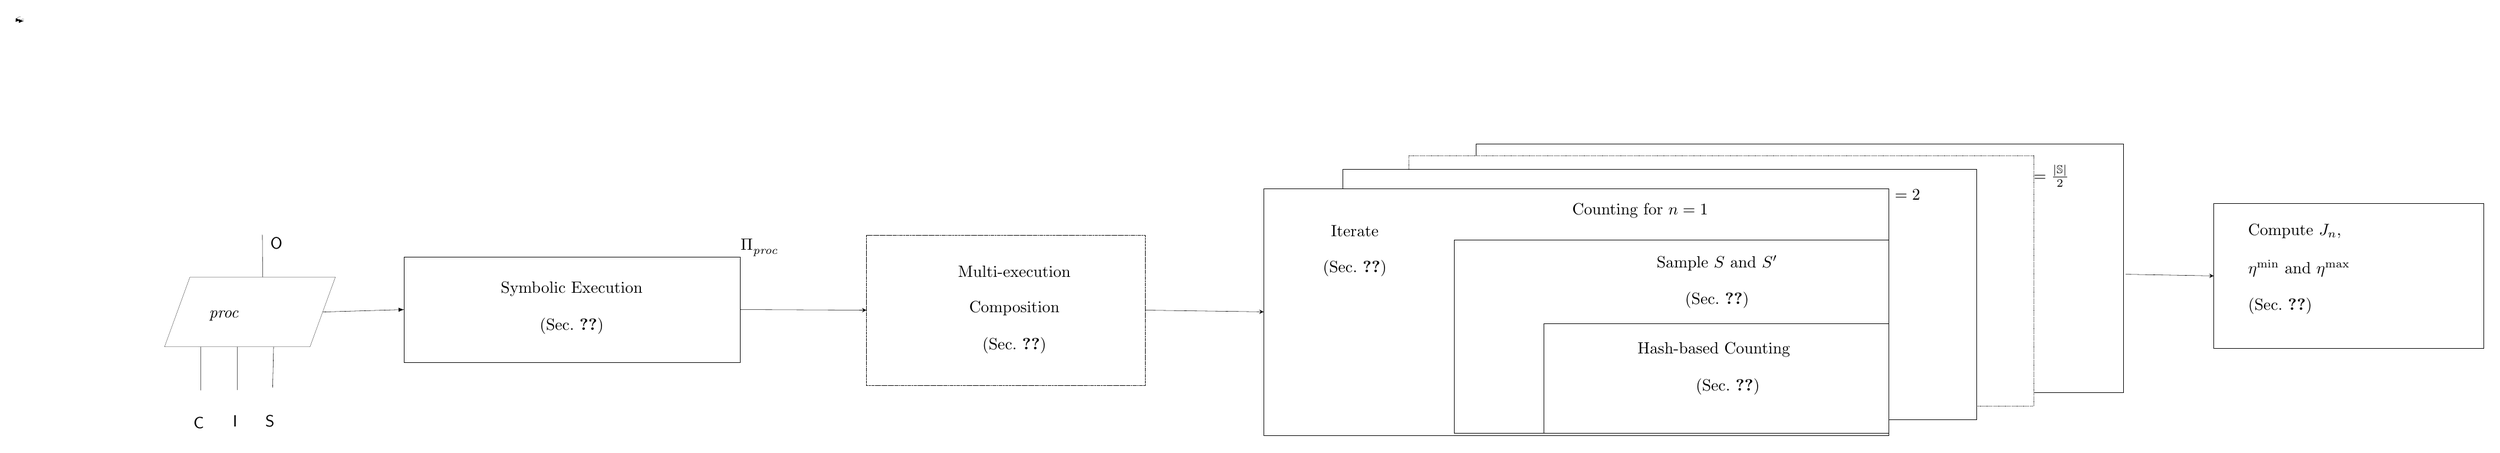
\begin{tikzpicture}
\pgftransformxscale{1.000000}
\pgftransformyscale{-1.000000}
\definecolor{dialinecolor}{rgb}{0.000000, 0.000000, 0.000000}
\pgfsetstrokecolor{dialinecolor}
\definecolor{dialinecolor}{rgb}{1.000000, 1.000000, 1.000000}
\pgfsetfillcolor{dialinecolor}
\definecolor{dialinecolor}{rgb}{1.000000, 1.000000, 1.000000}
\pgfsetfillcolor{dialinecolor}
\fill (32.472400\du,2.949270\du)--(32.472400\du,8.313852\du)--(46.411342\du,8.313852\du)--(46.411342\du,2.949270\du)--cycle;
\pgfsetlinewidth{0.100000\du}
\pgfsetdash{}{0pt}
\pgfsetdash{}{0pt}
\pgfsetmiterjoin
\definecolor{dialinecolor}{rgb}{0.000000, 0.000000, 0.000000}
\pgfsetstrokecolor{dialinecolor}
\draw (32.472400\du,2.949270\du)--(32.472400\du,8.313852\du)--(46.411342\du,8.313852\du)--(46.411342\du,2.949270\du)--cycle;
% setfont left to latex
\definecolor{dialinecolor}{rgb}{0.000000, 0.000000, 0.000000}
\pgfsetstrokecolor{dialinecolor}
\node at (39.441871\du,5.874747\du){};
\definecolor{dialinecolor}{rgb}{1.000000, 1.000000, 1.000000}
\pgfsetfillcolor{dialinecolor}
\fill (31.018700\du,3.200720\du)--(31.018700\du,8.603813\du)--(44.478732\du,8.603813\du)--(44.478732\du,3.200720\du)--cycle;
\pgfsetlinewidth{0.100000\du}
\pgfsetdash{{1.000000\du}{1.000000\du}}{0\du}
\pgfsetdash{{0.400000\du}{0.400000\du}}{0\du}
\pgfsetmiterjoin
\definecolor{dialinecolor}{rgb}{0.000000, 0.000000, 0.000000}
\pgfsetstrokecolor{dialinecolor}
\draw (31.018700\du,3.200720\du)--(31.018700\du,8.603813\du)--(44.478732\du,8.603813\du)--(44.478732\du,3.200720\du)--cycle;
% setfont left to latex
\definecolor{dialinecolor}{rgb}{0.000000, 0.000000, 0.000000}
\pgfsetstrokecolor{dialinecolor}
\node at (37.748716\du,6.145452\du){};
\definecolor{dialinecolor}{rgb}{1.000000, 1.000000, 1.000000}
\pgfsetfillcolor{dialinecolor}
\fill (29.597600\du,3.497390\du)--(29.597600\du,8.893773\du)--(43.250000\du,8.893773\du)--(43.250000\du,3.497390\du)--cycle;
\pgfsetlinewidth{0.100000\du}
\pgfsetdash{}{0pt}
\pgfsetdash{}{0pt}
\pgfsetmiterjoin
\definecolor{dialinecolor}{rgb}{0.000000, 0.000000, 0.000000}
\pgfsetstrokecolor{dialinecolor}
\draw (29.597600\du,3.497390\du)--(29.597600\du,8.893773\du)--(43.250000\du,8.893773\du)--(43.250000\du,3.497390\du)--cycle;
% setfont left to latex
\definecolor{dialinecolor}{rgb}{0.000000, 0.000000, 0.000000}
\pgfsetstrokecolor{dialinecolor}
\node at (36.423800\du,6.438768\du){};
\definecolor{dialinecolor}{rgb}{1.000000, 1.000000, 1.000000}
\pgfsetfillcolor{dialinecolor}
\fill (9.382400\du,5.382180\du)--(9.382400\du,7.663295\du)--(16.617400\du,7.663295\du)--(16.617400\du,5.382180\du)--cycle;
\pgfsetlinewidth{0.100000\du}
\pgfsetdash{}{0pt}
\pgfsetdash{}{0pt}
\pgfsetmiterjoin
\definecolor{dialinecolor}{rgb}{0.000000, 0.000000, 0.000000}
\pgfsetstrokecolor{dialinecolor}
\draw (9.382400\du,5.382180\du)--(9.382400\du,7.663295\du)--(16.617400\du,7.663295\du)--(16.617400\du,5.382180\du)--cycle;
% setfont left to latex
\definecolor{dialinecolor}{rgb}{0.000000, 0.000000, 0.000000}
\pgfsetstrokecolor{dialinecolor}
\node at (12.999900\du,6.765924\du){};
\definecolor{dialinecolor}{rgb}{1.000000, 1.000000, 1.000000}
\pgfsetfillcolor{dialinecolor}
\fill (4.767976\du,5.823180\du)--(7.901175\du,5.823180\du)--(7.353899\du,7.326808\du)--(4.220700\du,7.326808\du)--cycle;
\pgfsetlinewidth{0.100000\du}
\pgfsetdash{}{0pt}
\pgfsetdash{}{0pt}
\pgfsetmiterjoin
\definecolor{dialinecolor}{rgb}{0.000000, 0.000000, 0.000000}
\pgfsetstrokecolor{dialinecolor}
\draw (4.767976\du,5.823180\du)--(7.901175\du,5.823180\du)--(7.353899\du,7.326808\du)--(4.220700\du,7.326808\du)--cycle;
% setfont left to latex
\definecolor{dialinecolor}{rgb}{0.000000, 0.000000, 0.000000}
\pgfsetstrokecolor{dialinecolor}
\node at (6.060937\du,6.818180\du){};
\pgfsetlinewidth{0.200000\du}
\pgfsetdash{}{0pt}
\pgfsetdash{}{0pt}
\pgfsetbuttcap
{
\definecolor{dialinecolor}{rgb}{0.000000, 0.000000, 0.000000}
\pgfsetfillcolor{dialinecolor}
% was here!!!
\pgfsetarrowsend{latex}
\definecolor{dialinecolor}{rgb}{0.000000, 0.000000, 0.000000}
\pgfsetstrokecolor{dialinecolor}
\draw (7.627537\du,6.574994\du)--(9.382400\du,6.522740\du);
}
\pgfsetlinewidth{0.200000\du}
\pgfsetdash{}{0pt}
\pgfsetdash{}{0pt}
\pgfsetbuttcap
{
\definecolor{dialinecolor}{rgb}{0.000000, 0.000000, 0.000000}
\pgfsetfillcolor{dialinecolor}
% was here!!!
\pgfsetarrowsend{stealth}
\definecolor{dialinecolor}{rgb}{0.000000, 0.000000, 0.000000}
\pgfsetstrokecolor{dialinecolor}
\draw (16.617400\du,6.522740\du)--(19.338100\du,6.535535\du);
}
\pgfsetlinewidth{0.100000\du}
\pgfsetdash{}{0pt}
\pgfsetdash{}{0pt}
\pgfsetmiterjoin
\definecolor{dialinecolor}{rgb}{1.000000, 1.000000, 1.000000}
\pgfsetfillcolor{dialinecolor}
\fill (48.356300\du,4.232730\du)--(48.356300\du,7.361161\du)--(54.170223\du,7.361161\du)--(54.170223\du,4.232730\du)--cycle;
\definecolor{dialinecolor}{rgb}{0.000000, 0.000000, 0.000000}
\pgfsetstrokecolor{dialinecolor}
\draw (48.356300\du,4.232730\du)--(48.356300\du,7.361161\du)--(54.170223\du,7.361161\du)--(54.170223\du,4.232730\du)--cycle;
% setfont left to latex
\definecolor{dialinecolor}{rgb}{0.000000, 0.000000, 0.000000}
\pgfsetstrokecolor{dialinecolor}
\node[anchor=west] at (48.981400\du,4.835722\du){Compute \Jaccard{\secretsSetSize},};
% setfont left to latex
\definecolor{dialinecolor}{rgb}{0.000000, 0.000000, 0.000000}
\pgfsetstrokecolor{dialinecolor}
\node[anchor=west] at (48.981400\du,5.639350\du){\secretsSetSizeMin{} and \secretsSetSizeMax{}};
% setfont left to latex
\definecolor{dialinecolor}{rgb}{0.000000, 0.000000, 0.000000}
\pgfsetstrokecolor{dialinecolor}
\node[anchor=west] at (48.981400\du,6.442978\du){(\secref{sscf:sec:measurement:secretsSetSize})};
\pgfsetlinewidth{0.200000\du}
\pgfsetdash{}{0pt}
\pgfsetdash{}{0pt}
\pgfsetbuttcap
{
\definecolor{dialinecolor}{rgb}{0.000000, 0.000000, 0.000000}
\pgfsetfillcolor{dialinecolor}
% was here!!!
\pgfsetarrowsend{stealth}
\definecolor{dialinecolor}{rgb}{0.000000, 0.000000, 0.000000}
\pgfsetstrokecolor{dialinecolor}
\draw (46.461222\du,5.761787\du)--(48.356300\du,5.796946\du);
}
% setfont left to latex
\definecolor{dialinecolor}{rgb}{0.000000, 0.000000, 0.000000}
\pgfsetstrokecolor{dialinecolor}
\node[anchor=west] at (16.510700\du,5.187180\du){\postcondition{\proc}{}};
% setfont left to latex
\definecolor{dialinecolor}{rgb}{0.000000, 0.000000, 0.000000}
\pgfsetstrokecolor{dialinecolor}
\node at (12.990400\du,6.079380\du){Symbolic Execution};
% setfont left to latex
\definecolor{dialinecolor}{rgb}{0.000000, 0.000000, 0.000000}
\pgfsetstrokecolor{dialinecolor}
\node at (12.990400\du,6.879380\du){(\secref{sscf:sec:symbolic})};
\pgfsetlinewidth{0.200000\du}
\pgfsetdash{}{0pt}
\pgfsetdash{}{0pt}
\pgfsetbuttcap
{
\definecolor{dialinecolor}{rgb}{0.000000, 0.000000, 0.000000}
\pgfsetfillcolor{dialinecolor}
% was here!!!
\definecolor{dialinecolor}{rgb}{0.000000, 0.000000, 0.000000}
\pgfsetstrokecolor{dialinecolor}
\draw (5.003150\du,8.264880\du)--(5.004000\du,7.326808\du);
}
% setfont left to latex
\definecolor{dialinecolor}{rgb}{0.000000, 0.000000, 0.000000}
\pgfsetstrokecolor{dialinecolor}
\node at (4.965880\du,8.991080\du){\ACIFn{}};
% setfont left to latex
\definecolor{dialinecolor}{rgb}{0.000000, 0.000000, 0.000000}
\pgfsetstrokecolor{dialinecolor}
\node[anchor=west] at (5.059390\du,6.658680\du){\proc};
% setfont left to latex
\definecolor{dialinecolor}{rgb}{0.000000, 0.000000, 0.000000}
\pgfsetstrokecolor{dialinecolor}
\node[anchor=west] at (6.381450\du,5.115530\du){\AOOFn{}};
\pgfsetlinewidth{0.200000\du}
\pgfsetdash{}{0pt}
\pgfsetdash{}{0pt}
\pgfsetbuttcap
{
\definecolor{dialinecolor}{rgb}{0.000000, 0.000000, 0.000000}
\pgfsetfillcolor{dialinecolor}
% was here!!!
\definecolor{dialinecolor}{rgb}{0.000000, 0.000000, 0.000000}
\pgfsetstrokecolor{dialinecolor}
\draw (5.787800\du,8.258780\du)--(5.787299\du,7.326808\du);
}
\pgfsetlinewidth{0.200000\du}
\pgfsetdash{}{0pt}
\pgfsetdash{}{0pt}
\pgfsetbuttcap
{
\definecolor{dialinecolor}{rgb}{0.000000, 0.000000, 0.000000}
\pgfsetfillcolor{dialinecolor}
% was here!!!
\definecolor{dialinecolor}{rgb}{0.000000, 0.000000, 0.000000}
\pgfsetstrokecolor{dialinecolor}
\draw (6.550000\du,8.206690\du)--(6.570599\du,7.326808\du);
}
\pgfsetlinewidth{0.200000\du}
\pgfsetdash{}{0pt}
\pgfsetdash{}{0pt}
\pgfsetbuttcap
{
\definecolor{dialinecolor}{rgb}{0.000000, 0.000000, 0.000000}
\pgfsetfillcolor{dialinecolor}
% was here!!!
\definecolor{dialinecolor}{rgb}{0.000000, 0.000000, 0.000000}
\pgfsetstrokecolor{dialinecolor}
\draw (6.334575\du,5.823180\du)--(6.328330\du,4.907880\du);
}
\pgfsetlinewidth{0.200000\du}
\pgfsetdash{}{0pt}
\pgfsetdash{}{0pt}
\pgfsetbuttcap
{
\definecolor{dialinecolor}{rgb}{0.000000, 0.000000, 0.000000}
\pgfsetfillcolor{dialinecolor}
% was here!!!
\pgfsetarrowsend{stealth}
\definecolor{dialinecolor}{rgb}{0.000000, 0.000000, 0.000000}
\pgfsetstrokecolor{dialinecolor}
\draw (25.343300\du,6.535535\du)--(27.893800\du,6.571795\du);
}
\definecolor{dialinecolor}{rgb}{1.000000, 1.000000, 1.000000}
\pgfsetfillcolor{dialinecolor}
\fill (27.893800\du,3.911530\du)--(27.893800\du,9.232060\du)--(41.361737\du,9.232060\du)--(41.361737\du,3.911530\du)--cycle;
\pgfsetlinewidth{0.100000\du}
\pgfsetdash{}{0pt}
\pgfsetdash{}{0pt}
\pgfsetmiterjoin
\definecolor{dialinecolor}{rgb}{0.000000, 0.000000, 0.000000}
\pgfsetstrokecolor{dialinecolor}
\draw (27.893800\du,3.911530\du)--(27.893800\du,9.232060\du)--(41.361737\du,9.232060\du)--(41.361737\du,3.911530\du)--cycle;
% setfont left to latex
\definecolor{dialinecolor}{rgb}{0.000000, 0.000000, 0.000000}
\pgfsetstrokecolor{dialinecolor}
\node at (34.627768\du,6.814981\du){};
% setfont left to latex
\definecolor{dialinecolor}{rgb}{0.000000, 0.000000, 0.000000}
\pgfsetstrokecolor{dialinecolor}
\node[anchor=west] at (34.424500\du,4.395360\du){Counting for $\secretsSetSize{}=1$ };
\definecolor{dialinecolor}{rgb}{1.000000, 1.000000, 1.000000}
\pgfsetfillcolor{dialinecolor}
\fill (32.001000\du,5.015950\du)--(32.001000\du,9.183734\du)--(41.355875\du,9.183734\du)--(41.355875\du,5.015950\du)--cycle;
\pgfsetlinewidth{0.050000\du}
\pgfsetdash{}{0pt}
\pgfsetdash{}{0pt}
\pgfsetmiterjoin
\definecolor{dialinecolor}{rgb}{0.000000, 0.000000, 0.000000}
\pgfsetstrokecolor{dialinecolor}
\draw (32.001000\du,5.015950\du)--(32.001000\du,9.183734\du)--(41.355875\du,9.183734\du)--(41.355875\du,5.015950\du)--cycle;
% setfont left to latex
\definecolor{dialinecolor}{rgb}{0.000000, 0.000000, 0.000000}
\pgfsetstrokecolor{dialinecolor}
\node at (36.678438\du,7.343028\du){ };
\definecolor{dialinecolor}{rgb}{1.000000, 1.000000, 1.000000}
\pgfsetfillcolor{dialinecolor}
\fill (33.931800\du,6.820190\du)--(33.931800\du,9.183728\du)--(41.356599\du,9.183728\du)--(41.356599\du,6.820190\du)--cycle;
\pgfsetlinewidth{0.050000\du}
\pgfsetdash{}{0pt}
\pgfsetdash{}{0pt}
\pgfsetmiterjoin
\definecolor{dialinecolor}{rgb}{0.000000, 0.000000, 0.000000}
\pgfsetstrokecolor{dialinecolor}
\draw (33.931800\du,6.820190\du)--(33.931800\du,9.183728\du)--(41.356599\du,9.183728\du)--(41.356599\du,6.820190\du)--cycle;
% setfont left to latex
\definecolor{dialinecolor}{rgb}{0.000000, 0.000000, 0.000000}
\pgfsetstrokecolor{dialinecolor}
\node at (37.644200\du,8.245145\du){};
% setfont left to latex
\definecolor{dialinecolor}{rgb}{0.000000, 0.000000, 0.000000}
\pgfsetstrokecolor{dialinecolor}
\node at (37.591900\du,7.383960\du){Hash-based Counting };
% setfont left to latex
\definecolor{dialinecolor}{rgb}{0.000000, 0.000000, 0.000000}
\pgfsetstrokecolor{dialinecolor}
\node at (37.891900\du,8.183960\du){(\secref{sscf:sec:impl:hash:possibleDoubles})};
% setfont left to latex
\definecolor{dialinecolor}{rgb}{0.000000, 0.000000, 0.000000}
\pgfsetstrokecolor{dialinecolor}
\node[anchor=west] at (41.372500\du,4.052490\du){$=2$};
% setfont left to latex
\definecolor{dialinecolor}{rgb}{0.000000, 0.000000, 0.000000}
\pgfsetstrokecolor{dialinecolor}
\node[anchor=west] at (44.363000\du,3.638400\du){$=\frac{\setSize{\secretsDomain}}{2}$};
% setfont left to latex
\definecolor{dialinecolor}{rgb}{0.000000, 0.000000, 0.000000}
\pgfsetstrokecolor{dialinecolor}
\node at (37.661400\du,5.526480\du){Sample \secretsSet{} and \secretsSetAlt{} };
% setfont left to latex
\definecolor{dialinecolor}{rgb}{0.000000, 0.000000, 0.000000}
\pgfsetstrokecolor{dialinecolor}
\node at (37.661400\du,6.326480\du){(\secref{sscf:sec:impl:hash:secretsSetSize})};
\definecolor{dialinecolor}{rgb}{1.000000, 1.000000, 1.000000}
\pgfsetfillcolor{dialinecolor}
\fill (19.338100\du,4.917720\du)--(19.338100\du,8.153350\du)--(25.343300\du,8.153350\du)--(25.343300\du,4.917720\du)--cycle;
\pgfsetlinewidth{0.100000\du}
\pgfsetdash{{1.000000\du}{0.200000\du}{0.200000\du}{0.200000\du}{0.200000\du}{0.200000\du}}{0cm}
\pgfsetdash{{1.000000\du}{0.200000\du}{0.200000\du}{0.200000\du}{0.200000\du}{0.200000\du}}{0cm}
\pgfsetmiterjoin
\definecolor{dialinecolor}{rgb}{0.000000, 0.000000, 0.000000}
\pgfsetstrokecolor{dialinecolor}
\draw (19.338100\du,4.917720\du)--(19.338100\du,8.153350\du)--(25.343300\du,8.153350\du)--(25.343300\du,4.917720\du)--cycle;
% setfont left to latex
\definecolor{dialinecolor}{rgb}{0.000000, 0.000000, 0.000000}
\pgfsetstrokecolor{dialinecolor}
\node at (22.340700\du,6.778721\du){};
% setfont left to latex
\definecolor{dialinecolor}{rgb}{0.000000, 0.000000, 0.000000}
\pgfsetstrokecolor{dialinecolor}
\node at (22.525400\du,5.703560\du){Multi-execution };
% setfont left to latex
\definecolor{dialinecolor}{rgb}{0.000000, 0.000000, 0.000000}
\pgfsetstrokecolor{dialinecolor}
\node at (22.525400\du,6.503560\du){Composition};
% setfont left to latex
\definecolor{dialinecolor}{rgb}{0.000000, 0.000000, 0.000000}
\pgfsetstrokecolor{dialinecolor}
\node at (22.525400\du,7.303560\du){(\secref{sscf:sec:impl:multiround})};
% setfont left to latex
\definecolor{dialinecolor}{rgb}{0.000000, 0.000000, 0.000000}
\pgfsetstrokecolor{dialinecolor}
\node at (5.750000\du,8.956690\du){\AIIFn{}};
% setfont left to latex
\definecolor{dialinecolor}{rgb}{0.000000, 0.000000, 0.000000}
\pgfsetstrokecolor{dialinecolor}
\node at (6.500000\du,8.958370\du){\SecFn{}};
\pgfsetlinewidth{0.100000\du}
\pgfsetdash{}{0pt}
\pgfsetdash{}{0pt}
\pgfsetmiterjoin
\pgfsetbuttcap
{
\definecolor{dialinecolor}{rgb}{0.000000, 0.000000, 0.000000}
\pgfsetfillcolor{dialinecolor}
% was here!!!
\pgfsetarrowsend{latex}
\definecolor{dialinecolor}{rgb}{0.000000, 0.000000, 0.000000}
\pgfsetstrokecolor{dialinecolor}
\pgfpathmoveto{\pgfpoint{33.931800\du}{7.411075\du}}
\pgfpathcurveto{\pgfpoint{32.221400\du}{6.944315\du}}{\pgfpoint{32.124800\du}{8.602974\du}}{\pgfpoint{33.931800\du}{8.592844\du}}
\pgfusepath{stroke}
}
\pgfsetlinewidth{0.100000\du}
\pgfsetdash{}{0pt}
\pgfsetdash{}{0pt}
\pgfsetmiterjoin
\pgfsetbuttcap
{
\definecolor{dialinecolor}{rgb}{0.000000, 0.000000, 0.000000}
\pgfsetfillcolor{dialinecolor}
% was here!!!
\pgfsetarrowsend{latex}
\definecolor{dialinecolor}{rgb}{0.000000, 0.000000, 0.000000}
\pgfsetstrokecolor{dialinecolor}
\pgfpathmoveto{\pgfpoint{32.001000\du}{6.057896\du}}
\pgfpathcurveto{\pgfpoint{29.563500\du}{5.744576\du}}{\pgfpoint{29.321800\du}{7.975568\du}}{\pgfpoint{32.001000\du}{8.141788\du}}
\pgfusepath{stroke}
}
% setfont left to latex
\definecolor{dialinecolor}{rgb}{0.000000, 0.000000, 0.000000}
\pgfsetstrokecolor{dialinecolor}
\node at (29.858900\du,4.830340\du){Iterate};
% setfont left to latex
\definecolor{dialinecolor}{rgb}{0.000000, 0.000000, 0.000000}
\pgfsetstrokecolor{dialinecolor}
\node at (29.858900\du,5.630340\du){(\secref{sscf:sec:impl:modeling})};
\end{tikzpicture}
}
}
\vspace{-0.1in}
\caption[Workflow of evaluating leakage]{Workflow of evaluating leakage, from left to right: label the
  different types of inputs and outputs; generate postconditions
  \postcondition{\proc}{} using symbolic execution; optionally,
  compose multi-execution constraints; perform model counting for
  different sizes of \secretsSetSize{}; and generate our leakage
  measures}
\label{fig:workflow}
\end{figure*}

In this section, we discuss our implementation for computing the
measures discussed in \secref{sscf:sec:measure}. \figref{fig:workflow} shows
the overall workflow for doing so. \secref{sscf:sec:symbolic} illustrates
the use of symbolic execution (e.g.,
\cite{cadar08:klee,chipounov11:s2e}) for generating postconditions,
with a focus on a particular optimization that proved useful for our
case studies in \secref{sscf:sec:case-studies}.  At the core of our
implementation is the adaption of hash-based model counting
technique that is discussed in
\secrefs{sscf:sec:impl:hash}{sscf:sec:impl:modeling}.  In
\secref{sscf:sec:impl:multiround}, we present an adaptation for generating
logical postconditions for multiple rounds of procedure executions.

\iffalse
\begin{figure*}[t!]
\begin{subfigure}[b]{0.25\textwidth}
  \centering
	\resizebox{0.55\linewidth}{!}{\footnotesize\input{fig/proc.tex}}
  \caption{Procedure}
  \label{fig:mergingbenefit:proc}
\end{subfigure}
\begin{subfigure}[b]{0.37\textwidth}
  \centering
  \resizebox{0.92\linewidth}{!}{\scriptsize\input{fig/no-merge-pc-clean.tex}}
  \caption{Path exploration without merging}
  \label{fig:mergingbenefit:nomerge}
\end{subfigure}
\begin{subfigure}[b]{0.37\textwidth}
  \centering
  \resizebox{0.8\linewidth}{!}{\scriptsize\input{fig/merge-pc-clean.tex}}
  \caption{Path exploration with merging}
  \label{fig:mergingbenefit:merge}
\end{subfigure}
\caption{Benefits from state merging, discussed in \appref{sscf:sec:symbolic}}
\label{fig:mergingbenefit}
\end{figure*}
\fi

\subsection{From software procedure to logical postcondition}
\label{sscf:sec:symbolic}

As mentioned in \secref{sscf:sec:measurement}, the logical postcondition
\postcondition{\proc}{} represents the relationship between inputs and
outputs induced by procedure \proc. To extract \postcondition{\proc}{}
from \proc, we apply symbolic execution to \proc.  After marking each
input variable (i.e., each parameter in \ACIKeys, \AIIKeys,\footnote{To
  model the random input generated from random number generator
  $\mathit{rand}()$ in symbolic execution, we created a symbolic
  variable per $\mathit{rand}()$ function call as its returned
  value.} and \SecKeys) symbolic before the user-defined entry point,
we utilize \klee~\cite{cadar08:klee} or \stwoe~\cite{chipounov11:s2e}
to explore all feasible execution paths through \proc that reach a
\texttt{return}.  On each path through \proc, the symbolic execution
engine accumulates a set of constraints among symbolic variables
implied by the branches taken and assignments computed along that
path.  These constraints coupled with the assignments for $\AOOKeys$ defined by our API \texttt{make\_observable}, as accumulated through the \texttt{return}
instruction, form the postcondition for the path, and then
\postcondition{\proc}{} is simply the disjunction of the path
conditions generated for each execution path. 

Symbolic execution can suffer from state explosion, and so we
leveraged an optimization in our work to manage this explosion.
Specifically, we implemented a searcher to perform \textit{state merging}~\cite{Kuznetsov:2012:ESM} frequently,
wherein the constraints accumulated along two or more execution
prefixes ending at the same instruction are disjoined and then
simplified to the extent possible (using an SMT solver); execution is
then continued from their last instruction, accumulating more
constraints into their now-combined constraints.  In doing so, these
two execution prefixes need only be extended once, versus each being
extended separately if no merging occurred.

This optimization dramatically reduced the number of symbolic states
managed in one of our case studies in \secref{sscf:sec:case-studies:tcp}, improving the speed
of extracting \postcondition{\proc}{} by more than $600\times$.  For
this case study, we forced state merging to occur whenever a symbolic
state was forked at a symbolic branch.  To reduce the complexity of
the merged path constraint, however, we avoided merging two path
constraints when their expressions for the outputs in \AOOFn{}
differed or when two path constraints (in conjunctive normal form) had
less than half of their conjuncts in common.

To correctly measure the leakage, we assume the postcondition
$\postcondition{\proc}{}(\ACIFn{}, \AIIFn{}, \SecFn{}, \AOOFn{})$ is
complete and sound.  Completeness means that if $\langle \ACIFn{},
\AIIFn{}, \SecFn{}, \AOOFn{}\rangle$ is feasible for \proc, then
$\langle \ACIFn{}, \AIIFn{}, \SecFn{}, \AOOFn{}\rangle$ satisfies
$\postcondition{\proc}{}(\ACIFn{}, \AIIFn{}, \SecFn{}, \AOOFn{})$.
Soundness requires that if $\langle \ACIFn{}, \AIIFn{}, \SecFn{},
\AOOFn{}\rangle$ is infeasible for \proc, then $\langle \ACIFn{},
\AIIFn{}, \SecFn{}, \AOOFn{}\rangle$ does not satisfy
$\postcondition{\proc}{}(\ACIFn{}, \AIIFn{}, \SecFn{}, \AOOFn{})$.  A
well-known limitation of symbolic execution is how to manage unbounded
loops, since these can prevent symbolic execution from terminating.
In the case studies of \secref{sscf:sec:case-studies} we bounded all
inputs, which was enough in these case studies to ensure that symbolic
execution terminated.  Provided that we bound the input parameters
sufficiently loosely to encompass all values they can take on in
practice, this bounding does not impact the assessment provided by our
measures in practice.

\begin{table}
  \centering
  \caption{Postcondition generation times for case studies}
  \label{tab:symex}
  {\small
  		\setlength\tabcolsep{0.6ex}
    \begin{tabular}{clcccc}
      \toprule
      \textbf{Sec.} & \multicolumn{1}{c}{\textbf{Procedure}} & \parbox[m]{2.5em}{\centering\klee \\ $\times 1$} & \parbox[m]{2.5em}{\centering\klee \\ $\times 16$} & \parbox[m]{5.8em}{\centering\klee \\ $\times 1$, merging} & \parbox[m]{2em}{\centering\stwoe \\ $\times 16$} \\
      \midrule
      \ref{sscf:sec:case-studies:sphinx} & Auto-complete & 2\days & 12\hours \\
      \ref{sscf:sec:case-studies:crime} & \gzip & 3\days & 21\hours & & 8\hours \\
      \ref{sscf:sec:case-studies:crime} & \smaz & 2\days & 18\hours & & 6\hours \\
      \ref{sscf:sec:case-studies:tcp} & v3.18 & 7\days & 4\days & 17\mins \\
      \ref{sscf:sec:case-studies:tcp} & v3.18-patched & & & 18\mins \\
      \ref{sscf:sec:case-studies:tcp} & v3.18-rmCounter & & & 17\mins \\
      \bottomrule
    \end{tabular}
  }
\end{table}

Postcondition generation costs are summarized in \figref{tab:symex}.
These computations were performed on a DELL PowerEdge R710 server
equipped with two 2.67\gigahertz Intel Xeon 5550 processors and
128\gigabytes memory. Each processor includes 4 physical cores and had
hyperthreading enabled.  As indicated in \figref{tab:symex}, we
experimented with both \klee and \stwoe to generate postconditions,
depending on the procedure.  In the column headings, a `$\times 1$' or
`$\times 16$' indicates the number of processes across which the
computation was divided.  To enable multi-process support in \klee
(i.e., `$\times 16$'), we made a small modification in \klee's
execution engine, to cause it to explore only execution paths starting
from a predefined branching prefix.  The designation `merging'
indicates the use of the \klee optimization summarized above; as
indicated in \figref{tab:symex}, this optimization was remarkably
effective on the Linux TCP implementations discussed
in \secref{sscf:sec:case-studies:tcp}.  \stwoe was configured to utilize
its concolic execution capabilities.

\subsection{Hash-based model counting for \Jaccard{\secretsSetSize}}
\label{sscf:sec:impl:hash}

To calculate \Jaccard{\secretsSetSize}, we need to estimate
$\setSize{\possibleDoubles{\secretsSet{}} \cap
  \possibleDoubles{\secretsSetAlt{}}}$ and
$\setSize{\possibleDoubles{\secretsSet{}} \cup
  \possibleDoubles{\secretsSetAlt{}}}$ for randomly selected, disjoint
sets \secretsSet{} and \secretsSetAlt{} of size \secretsSetSize. Since 
\begin{align}
\setSize{\possibleDoubles{\secretsSet{}} \cap \possibleDoubles{\secretsSetAlt{}}}
& = \setSize{\possibleDoubles{\secretsSet{}}}
  + \setSize{\possibleDoubles{\secretsSetAlt{}}}
  - \setSize{\possibleDoubles{\secretsSet{}} \cup \possibleDoubles{\secretsSetAlt{}}}
  & \mathrm{and}
  \label{eqn:intersection}\\
\setSize{\possibleDoubles{\secretsSet{}} \cup \possibleDoubles{\secretsSetAlt{}}}
& = \setSize{\possibleDoubles{\secretsSet{} \cup \secretsSetAlt{}}},
  \label{eqn:union}
\end{align}
to estimate \Jaccard{\secretsSetSize} it suffices to estimate
\setSize{\possibleDoubles{\secretsSetAltAlt{}}} for specified sets
\secretsSetAltAlt{} (i.e., $\secretsSetAltAlt{} = \secretsSet{}$,
$\secretsSetAltAlt{} = \secretsSetAlt{}$, or $\secretsSetAltAlt{} =
\secretsSet{} \cup \secretsSetAlt{}$). In this section, we provide two
optimizations for producing such estimates.

\subsubsection{Estimating \setSize{\possibleDoubles{\secretsSet{}}}}
\label{sscf:sec:impl:hash:possibleDoubles}
Our first optimization is an adaptation of the approximate model
counting technique due to Chakraborty et
al.~\cite{Chakraborty:2013:SAM:2961240.2961265}~(see \secref{sec:related:qif:approxcount}).

We estimate \setSize{\possibleDoubles{\secretsSet{}}} through a
similar algorithm used in projected model counting, i.e., by
iteratively selecting \hashPrefixFn{\hashFnOutputPrefixBits} and
$\hashFnOutputPrefix \in \{0,1\}^{\hashFnOutputPrefixBits}$ at
random, but apply the hash function only to the \ACIFn{} and \AOOFn{}
values of a satisfying assignment for \postcondition{\proc}{}.  More
specifically, we compute the set
\[
\possibleDoublesSubset{\secretsSet{}}{\hashFnOutputPrefix}{}
= \left\{\langle\ACIFn{}, \AOOFn{}\rangle ~\left|~
  \langle\ACIFn{}, \AOOFn{}\rangle \in \possibleDoubles{\secretsSet{}} \wedge
    \hashPrefixFn{\hashFnOutputPrefixBits}(\langle\ACIFn{},
    \AOOFn{}\rangle) = \hashFnOutputPrefix
    \right.\right\}
\]

That is, $\possibleDoublesSubset{\secretsSet{}}{\hashFnOutputPrefix}{}
\subseteq \possibleDoubles{\secretsSet{}}$ contains the elements of
\possibleDoubles{\secretsSet{} } whose hash is \hashFnOutputPrefix.
Intuitively, this yields an estimate
\begin{align}
\setSize{\possibleDoubles{\secretsSet{}}} \approx
2^{\hashFnOutputPrefixBits} \cdot
\setSize{\possibleDoublesSubset{\secretsSet{}}{\hashFnOutputPrefix}{}}
\label{eqn:possibleDoublesEstimate}
\end{align}
To reach an estimate of confidence \confidence, we generate a number
of $\langle \hashFnOutputPrefixBits, \hashFnOutputPrefix,
\hashFnOutputPrefixAlt\rangle$ triples such that
\begin{align}
 \setSize{\possibleDoublesSubset{\secretsSet{}}{\hashFnOutputPrefix}{}}\leq\pivot \textrm{ and } 
\setSize{\possibleDoublesSubset{\secretsSet{}}{\hashFnOutputPrefixAlt}{}}>\pivot 
\label{eqn:pivot}
\end{align}
where $\hashFnOutputPrefix \in \{0,1\}^{\hashFnOutputPrefixBits}$,
$\hashFnOutputPrefixAlt \in \{0,1\}^{\hashFnOutputPrefixBits-1}$, and
\pivot is derived from
\error~\cite{Chakraborty:2013:SAM:2961240.2961265}.  Each such triple
individually provides an estimate that is within error \error with
confidence at least
$0.78$~\cite[Lemma~1]{Chakraborty:2013:SAM:2961240.2961265}, and the
median of the estimates for all such triples is within error \error
with confidence that can be increased arbitrarily with more
$\langle
\hashFnOutputPrefixBits, \hashFnOutputPrefix,
\hashFnOutputPrefixAlt\rangle$ such triples.  As a special case, if
$\setSize{\possibleDoublesSubset{\secretsSet{}}{\hashFnOutputPrefix}{}}
\le \pivot$ at $\hashFnOutputPrefixBits=0$, then
\setSize{\possibleDoublesSubset{\secretsSet{}}{\hashFnOutputPrefix}{}}
is an exact count of \setSize{\possibleDoubles{\secretsSet{}}} since
$\possibleDoublesSubset{\secretsSet{}}{\hashFnOutputPrefix}{} =
\possibleDoubles{\secretsSet{}}$.

\subsubsection{Sampling \secretsSet{}, \secretsSetAlt{} of Expected
  Size \secretsSetSize}
\label{sscf:sec:impl:hash:secretsSetSize}

A second expense of calculating \possibleDoubles{\secretsSet{}} and
\possibleDoubles{\secretsSetAlt{}} explicitly is in enumerating
\secretsSet{} and \secretsSetAlt{} themselves, especially if
\secretsSetSize is large.  We can leverage hashing similarly to the
method above to avoid enumerating \secretsSet{} and \secretsSetAlt{}
directly for {$\secretsSetSize = \setSize{\secretsDomain}/2^{\hashFnOutputPrefixBits}$} for some
$\hashFnOutputPrefixBits \ge 0$.

Specifically, to estimate \Jaccard{\secretsSetSize} for
{$\secretsSetSize = \setSize{\secretsDomain}/2^{\hashFnOutputPrefixBits}$}, we select
\hashPrefixFn{\hashFnOutputPrefixBits} and $\hashFnOutputPrefix \in
\{0,1\}^{\hashFnOutputPrefixBits-1}$ at random and, for each such
selection, define
\begin{align*}
  \possibleTriplesByPrefix{\hashFnOutputPrefix}{0} & = \left\{\langle\ACIFn{}, \AOOFn{},
  \AIIFn{}\rangle ~\left|~ \exists \SecFn{} :
  \postcondition{\proc}{}(\ACIFn{}, \AIIFn{}, \SecFn{}, \AOOFn{}) \wedge
  \hashPrefixFn{\hashFnOutputPrefixBits}(\SecFn{}) = \concat{\hashFnOutputPrefix}{0}\right.\right\} \\
    \possibleTriplesByPrefix{\hashFnOutputPrefix}{1} & = \left\{\langle\ACIFn{}, \AOOFn{},
  \AIIFn{}\rangle ~\left|~ \exists \SecFn{} :
  \postcondition{\proc}{}(\ACIFn{}, \AIIFn{}, \SecFn{}, \AOOFn{}) \wedge
  \hashPrefixFn{\hashFnOutputPrefixBits}(\SecFn{}) = \concat{\hashFnOutputPrefix}{1}\right.\right\} \\
    \possibleTriplesByPrefix{\hashFnOutputPrefix}{} & = \left\{\langle\ACIFn{}, \AOOFn{},
  \AIIFn{}\rangle ~\left|~ \exists \SecFn{} :
  \postcondition{\proc}{}(\ACIFn{}, \AIIFn{}, \SecFn{}, \AOOFn{}) \wedge
  \hashPrefixFn{\hashFnOutputPrefixBits-1}(\SecFn{}) = \hashFnOutputPrefix\right.\right\}
\end{align*}
where \hashPrefixFn{\hashFnOutputPrefixBits-1} denotes the function
\hashPrefixFn{\hashFnOutputPrefixBits} but dropping the rightmost bit
from the output.  Then, we use the sets
\begin{align*}
  \possibleDoublesByPrefix{\hashFnOutputPrefix}{0}
  & = \left\{\langle\ACIFn{}, \AOOFn{}\rangle ~\left|~
      \exists \AIIFn{}: \langle\ACIFn{}, \AOOFn{}, \AIIFn{} \rangle \in
      \possibleTriplesByPrefix{\hashFnOutputPrefix}{0}
      \right.\right\}\\
  \possibleDoublesByPrefix{\hashFnOutputPrefix}{1}
  & = \left\{\langle\ACIFn{}, \AOOFn{}\rangle ~\left|~
      \exists \AIIFn{}: \langle\ACIFn{}, \AOOFn{}, \AIIFn{} \rangle \in
      \possibleTriplesByPrefix{\hashFnOutputPrefix}{1}
      \right.\right\} \\
  \possibleDoublesByPrefix{\hashFnOutputPrefix}{}
  & = \left\{\langle\ACIFn{}, \AOOFn{}\rangle ~\left|~
      \exists \AIIFn{}: \langle\ACIFn{}, \AOOFn{}, \AIIFn{} \rangle \in
      \possibleTriplesByPrefix{\hashFnOutputPrefix}{}
      \right.\right\}
\end{align*}
in place of \possibleDoubles{\secretsSet{}},
\possibleDoubles{\secretsSetAlt{}}, and
\possibleDoubles{\secretsSet{}\cup\secretsSetAlt{}}, respectively, to
perform the calculations \eqnsref{eqn:intersection}{eqn:union}.  And,
of course, the optimization in \secref{sscf:sec:impl:hash:possibleDoubles}
can be used in conjunction with this approach, e.g., computing
\begin{align}
\possibleDoublesSubset{\hashFnOutputPrefix}{\hashFnOutputPrefixAlt}{0}
= \left\{\langle\ACIFn{}, \AOOFn{}\rangle ~\left|~
  \langle\ACIFn{}, \AOOFn{}\rangle \in \possibleDoublesByPrefix{\hashFnOutputPrefix}{0} \wedge
    \hashPrefixFnAlt{\hashFnOutputPrefixBitsAlt}(\langle\ACIFn{},\AOOFn{}\rangle) = \hashFnOutputPrefixAlt
    \right.\right\}
\label{eqn:toCount}
\end{align}
for a different, random hash function
\hashPrefixFnAlt{\hashFnOutputPrefixBitsAlt} and random prefix
$\hashFnOutputPrefixAlt \in \{0,1\}^{\hashFnOutputPrefixBitsAlt}$.  We
then use the algorithm summarized in
\secref{sscf:sec:impl:hash:possibleDoubles} to estimate
\setSize{\possibleDoublesByPrefix{\hashFnOutputPrefix}{0}}.

Two more points about this algorithm warrant emphasis:
\begin{compactitem}
\item Because our algorithm explicitly enumerates the contents of each
  \possibleDoublesSubset{\hashFnOutputPrefix}{\hashFnOutputPrefixAlt}{0}
  and
  \possibleDoublesSubset{\hashFnOutputPrefix}{\hashFnOutputPrefixAlt}{1},
  when leakage is detected (i.e., $\Jaccard{\secretsSetSize} > 0$ for
  some \secretsSetSize) these sets can be used to identify
  $\langle\ACIFn{}, \AOOFn{}\rangle$ pairs that are in
  $\possibleDoublesByPrefix{\hashFnOutputPrefix}{0} \setminus
  \possibleDoublesByPrefix{\hashFnOutputPrefix}{1}$ or
  $\possibleDoublesByPrefix{\hashFnOutputPrefix}{1} \setminus
  \possibleDoublesByPrefix{\hashFnOutputPrefix}{0}$.  These examples
  can guide developers in understanding the reason for the leakage and
  in mitigating the problem.
\item Because the number of secrets with a random
  length-\hashFnOutputPrefixBits hash prefix \hashFnOutputPrefix is
  only of \textit{expected} size $\secretsSetSize =
  \setSize{\secretsDomain}/2^{\hashFnOutputPrefixBits}$, for the rest
of the chapter we use a
  definition of \Jaccard{\secretsSetSize} as in \eqnref{dfn:jaccard}
  but weakened so that \setSize{\secretsSet{}} and
  \setSize{\secretsSetAlt{}} equal \secretsSetSize in expectation.
\end{compactitem}

\subsection{Hash-based model counting for \JaccardRand{\secretsSetSize}}
\label{sscf:sec:impl:hashTriples}
The calculations of the previous section require some modifications
when we are instead computing \JaccardRand{\secretsSetSize} for
{$\secretsSetSize = \setSize{\secretsDomain}/2^{\hashFnOutputPrefixBits}$}.  Similar to the
previous section, we can use
\possibleTriplesByPrefix{\hashFnOutputPrefix}{} for
$\hashFnOutputPrefix \in \{0,1\}^{\hashFnOutputPrefixBits-1}$ in place
of $\possibleTriples{\secretsSet{}}\cup\possibleTriples{\secretsSetAlt{}}=\possibleTriples{\secretsSet{}\cup\secretsSetAlt{}}$.
However, to estimate
\setSize{\possibleTriplesIntersect{\secretsSet{}}{\secretsSetAlt{}}}
for a random \secretsSet{} and \secretsSetAlt{}, we need a different
approach.  Specifically, we calculate
\setSize{\possibleTriplesIntersect{\secretsSet{}}{\secretsSetAlt{}}}
by estimating the size of
\begin{align*}
\possibleTriplesIntersectByPrefix{\hashFnOutputPrefix} 
& = \left\{\langle\ACIFn{}, \AOOFn{}, \AIIFn{}\rangle ~\left|
     \begin{array}[m]{rl}
       \exists \SecFn{},\SecFnAlt{},\AIIFnAlt{}: &
       \postcondition{\proc}{}(\ACIFn{}, \AIIFn{}, \SecFn{}, \AOOFn{})~\wedge 
        \postcondition{\proc}{}(\ACIFn{}, \AIIFnAlt{},\SecFnAlt{}, \AOOFn{})~\wedge \\
       & \hashPrefixFn{\hashFnOutputPrefixBits}(\SecFn{}) = \concat{\hashFnOutputPrefix}{0}~\wedge 
        \hashPrefixFn{\hashFnOutputPrefixBits}(\SecFnAlt{}) = \concat{\hashFnOutputPrefix}{1}
\end{array}\right.\right\}
\end{align*}
since $\langle\ACIFn{}, \AOOFn{}, \AIIFn{}\rangle \in
\possibleTriplesIntersectByPrefix{\hashFnOutputPrefix}$ iff
$\langle\ACIFn{}, \AOOFn{}, \AIIFn{}\rangle \in
\possibleTriplesByPrefix{\hashFnOutputPrefix}{0}$ and
$\langle\ACIFn{}, \AOOFn{}\rangle \in
\possibleDoublesByPrefix{\hashFnOutputPrefix}{0} \cap
\possibleDoublesByPrefix{\hashFnOutputPrefix}{1}$.  This method does
come at considerably greater computational cost, however, due to the
duplication of the constraints \postcondition{\proc}{} in the
specification of this set.  We will demonstrate this in our case
studies in \secref{sscf:sec:case-studies}.

\subsection{Parameter settings for computing
\Jaccard{\secretsSetSize} and \JaccardRand{\secretsSetSize}}
\label{sscf:sec:impl:modeling}
In the hash-based model counting described above, we use the 3-wise
independent hash functions suggested by Chakraborty et
al.~\cite{Chakraborty:2013:SAM:2961240.2961265}, and due to the large
number of XOR clauses in the resulting hash constraints, we use
\cryptominisat~\cite{soos2016cryptominisat} to enumerate the elements
of each
\possibleDoublesSubset{\hashFnOutputPrefix}{\hashFnOutputPrefixAlt}{}.
To reduce the complexity of the hash constraints, we concretize their
constant bits to minimize the independent
support~\cite{ivrii2016computing} before generating XOR clauses.
Multiple estimates of the form in
\eqnref{eqn:possibleDoublesEstimate}, for various values of
\hashFnOutputPrefixBits (in \eqnref{eqn:possibleDoublesEstimate}, or
respectively \hashFnOutputPrefixBitsAlt in \eqnref{eqn:toCount}), as
prescribed by Chakraborty et al., are used to estimate
\setSize{\possibleDoubles{\hashFnOutputPrefix}}.  We parameterized
this algorithm with error $\error = 0.45$ and confidence either
$\confidence = 0.99$ in \secref{sscf:sec:micro} or $\confidence = 0.92$ in
\secref{sscf:sec:case-studies},\footnote{The error bound of Chakroborty et
  al.\ is conservative; e.g., the results for 95 benchmarks showed
  less than 5\% error in practice even when using $\error = 0.75$
  \cite{Chakraborty:2013:SAM:2961240.2961265}.} for which 50 or 5
$\langle \hashFnOutputPrefixBits, \hashFnOutputPrefix,
\hashFnOutputPrefixAlt\rangle$ triples satisfying \eqnref{eqn:pivot}
sufficed, respectively.

We estimate \Jaccard{\secretsSetSize} as the sample mean of
$\Jaccard{}(\secretsSet{}, \secretsSetAlt{})$ for sampled pairs
\secretsSet{}, \secretsSetAlt{} of expected size \secretsSetSize
(i.e., defined by a $\hashFnOutputPrefix \in
\{0,1\}^{\hashFnOutputPrefixBits-1}$ for {$\secretsSetSize =
\setSize{\secretsDomain}/2^{\hashFnOutputPrefixBits}$}).  For each
\secretsSetSize we computed \Jaccard{\secretsSetSize} using a number
of sampled pairs \secretsSet{}, \secretsSetAlt{} equal to the larger
of 100 and the minimum needed so that the standard error was within
$5\%$ of the sample mean.

In addition, since \Jaccard{\secretsSetSize} is only an
estimate and so is subject to error and since that error is
influential in the calculation of \secretsSetSizeMax{} or
\secretsSetSizeMin{} especially when \secretsSetSize{} is small, we
round any $\Jaccard{\secretsSetSize} \le 0.025$ down to zero when
calculating the measures.  \JaccardRand{\secretsSetSize} is computed
similarly.

\subsection{Logical postconditions for multiple procedure executions}
\label{sscf:sec:impl:multiround}
In some scenarios it is insightful to observe the behavior of
\Jaccard{\secretsSetSize} for a procedure \proc when it is executed multiple times.
That is, consider a scenario in which \proc is executed \roundNmbr
times, possibly with relationships among the outputs of one execution
and the inputs of another, or simply among the inputs to different
executions.  Suppose these executions are denoted
\begin{align*}
  \AOOFn{1} & \gets \proc(\ACIFn{1}, \AIIFn{1}, \SecFn{1}) \\
  \AOOFn{2} & \gets \proc(\ACIFn{2}, \AIIFn{2}, \SecFn{2}) \\
         & \cdots \\
  \AOOFn{\roundNmbr} & \gets \proc(\ACIFn{\roundNmbr}, \AIIFn{\roundNmbr}, \SecFn{\roundNmbr})
\end{align*}
and that the postcondition of the \roundIdx-th invocation in isolation
is denoted \postcondition{\proc}{\roundIdx} (i.e.,
\postcondition{\proc}{\roundIdx} is simply \postcondition{\proc}{}
over the variables represented in \ACIFn{\roundIdx},
\AIIFn{\roundIdx}, \SecFn{\roundIdx}, and \AOOFn{\roundIdx}).  Then
the relationships among inputs and outputs can be described using
additional, manually constructed constraints
\glueConstraints{\proc}{1\ldots\roundNmbr}.  For example, if the
secret input to each execution of \proc is the same, then
\glueConstraints{\proc}{1\ldots\roundNmbr} would include the statement
that \secretVar has the same value in each execution (i.e.,
$\SecFn{1}(\secretVar) = \SecFn{2}(\secretVar) = \ldots =
\SecFn{\roundNmbr}(\secretVar)$).  Repeating our analysis for the
  ``procedure'' represented by the postcondition
\[
\left(\bigwedge_{\roundIdx=1}^{\roundNmbr} \postcondition{\proc}{\roundIdx} \right)
\wedge \glueConstraints{\proc}{1\ldots\roundNmbr}
\]
can reveal leakage that increases as the procedure is executed
multiple times.  We will see an example in \secref{sscf:sec:case-studies}.

\section{Microbenchmark Evaluation}
\label{sscf:sec:micro}

In this section we evaluate our methodology on artificially small
examples to illustrate its features.

\subsection{Leaking more about secret values vs.\ leaking about more secret values}
\label{sscf:sec:micro:nmbrVsAmount}
\begin{figure*}
\begin{subfigure}[b]{0.25\textwidth}
{\small
\begin{tabbing}
** \= ** \= \kill
\proc(\ACIFn{}, \AIIFn{}, \SecFn{}) \\
\>  if ($\SecFn{}(\secretVar)\!\bmod\!\modulus = 0$) \\
\> \> $\AOOFn{}(\textrm{`result'})\!\gets\!\SecFn{}(\secretVar)$ \\
\>  else \\
\> \>  $\AOOFn{}(\textrm{`result'})\!\gets\!0$\\
\> return \AOOFn{} \\[2ex]
\end{tabbing}
}
\caption{Procedure}
\label{fig:modcheckout:code}
\end{subfigure}
\begin{subfigure}[b]{0.385\textwidth}
\hspace{-1ex}
\resizebox{0.99\textwidth}{!}{\large\input{fig/sscf/modcheckout.tex}}
\caption{\Jaccard{\secretsSetSize} for different \secretsSetSize and \modulus}
\label{fig:modcheckout:Jaccard}
\end{subfigure}
%
\begin{subfigure}[b]{0.3\textwidth}
\DTLloaddb[noheader=true]{dbmodcheckout}{fig/sscf/modcheckout-0.csv}
\centering
\footnotesize{
\begin{tabular}{lcc}\toprule
\modulus & {\logSecretsSetSizeMin}& {\logSecretsSetSizeMax}\\ 
\midrule
\DTLforeach{dbmodcheckout}{\m=Column1,\nmin=Column2,\nmax=Column3}{\m & \nmin & \nmax \tabularnewline}
\\[-\normalbaselineskip]\bottomrule
\end{tabular}
}
\vspace{0.5em}
\caption{\hspace{-0.5em}\secretsSetSizeMin{} and \secretsSetSizeMax{} for different \modulus}
\label{fig:modcheckout:tbl}
\end{subfigure}
\caption{A procedure that leaks about more secrets as \modulus is decreased (see \secref{sscf:sec:micro:nmbrVsAmount})}
\label{fig:modcheckout}
\end{figure*}
\begin{figure*}
\begin{subfigure}[b]{0.26\textwidth}
\centering
\footnotesize{
\begin{tabbing}
** \= ** \= ** \= \kill
\proc(\ACIFn{}, \AIIFn{}, \SecFn{}) \\
\> $\AOOFn{}(\textrm{`result'}) \gets$ \\
\>\>\> $\SecFn{}(\secretVar) \bmod \modulus$ \\
\> return \AOOFn{} \\[7ex]
\end{tabbing}
}
\caption{Procedure\label{fig:modout:code}}
\end{subfigure}%
\begin{subfigure}[b]{0.405\textwidth}
\hspace{-1ex}
\resizebox{0.99\textwidth}{!}{\large\input{fig/sscf/modout.tex}}
\caption{\Jaccard{\secretsSetSize} for different \secretsSetSize and \modulus}
\label{fig:modout:Jaccard}
\end{subfigure}%
\begin{subfigure}[b]{0.3\textwidth}
\footnotesize{
\DTLloaddb[noheader=true]{dbmodout}{fig/sscf/modout-0.csv}
\centering
\begin{tabular}{lcc}\toprule
\modulus & {\logSecretsSetSizeMin}& {\logSecretsSetSizeMax}\\ 
\midrule
\DTLforeach{dbmodout}{\m=Column1,\nmin=Column2,\nmax=Column3}{\m & \nmin & \nmax \tabularnewline}
\\[-\normalbaselineskip]\bottomrule
\multicolumn{3}{l}{\parbox{0.95\linewidth}{\scriptsize``nan'' denotes
    ``not a number,'' i.e., $\secretsSetSizeMin{} = 0$ or
    $\secretsSetSizeMax{} = 0$}}
\end{tabular}
}
\vspace{0.5em}
\caption{\hspace{-0.5em}\secretsSetSizeMin{} and \secretsSetSizeMax{} for different \modulus}
\label{fig:modout:tbl}
\end{subfigure}
\caption{A procedure that leaks more about secret values as \modulus is increased (see \secref{sscf:sec:micro:nmbrVsAmount})}
\label{fig:modout}
\end{figure*}

In \secref{sscf:sec:measurement:secretsSetSize}, we showed through an
idealized example how a small \secretsSetSize is more useful for
evaluating the number of secrets about which information leaks,
whereas a large \secretsSetSize is more useful for evaluating the
amount of information leaked about these secrets.  Now we will use two
simple procedures with a controllable constant \modulus to
quantitatively demonstrate the necessity of varying \secretsSetSize
and the correct usage of \secretsSetSizeMin{} and
\secretsSetSizeMax{}.

The first procedure, shown in \figref{fig:modcheckout:code}, returns
the secret value if it is divisible by a constant $\modulus$ and
returns zero otherwise, where both $\SecFn{}(\secretVar)$ and \modulus
are 32-bit integers.  This procedure leaks the same amount of
information (the whole secret) about a larger number of secret values
if \modulus is decreased.  The behavior of \Jaccard{\secretsSetSize}
shown in \figref{fig:modcheckout:Jaccard} is consistent with this
observation.  Specifically, different values of \modulus induce curves
for \Jaccard{\secretsSetSize} that differ primarily in the minimum
value of \secretsSetSize where \Jaccard{\secretsSetSize} is large.
This behavior is also seen in the value of \secretsSetSizeMin{} in
\figref{fig:modcheckout:tbl}, where \secretsSetSizeMin{} ranges from
$\secretsSetSizeMin{} \approx 0$ at $\modulus = 2^{31}$ to
$\secretsSetSizeMin{} = 1$ at $\modulus = 1$.

Contrast this case with the procedure shown in
\figref{fig:modout:code}, which returns the residue class of the
secret value modulo a constant value \modulus.  As such, as \modulus
is increased, more information about each secret is leaked.  This is
demonstrated in \figref{fig:modout:Jaccard}, where the curves for
different values of \modulus differ in primarily in the maximum value
\secretsSetSize at which \Jaccard{\secretsSetSize} is large.
Similarly, \secretsSetSizeMax{} ranges from $\secretsSetSizeMax{} = 0$
at $\modulus = 1$ to $\secretsSetSizeMax{} \approx
2^{-0.8} \approx 0.57$ at $\modulus = 2^{31}$.

An example that blends these the previous two examples is show in in
\figref{fig:modcheck:code}; here the procedure returns $1$ if
$\SecFn{}(\secretVar) \bmod \modulus = \ACIFn{}(\textrm{`test'})$ and
$0$ otherwise, where \modulus is a 32-bit constant.  As such, this
procedure leaks a lot about a few secret values when \modulus is
large, and a little about many secret values when \modulus is small.
As shown in the $\roundNmbr=1$ columns of \figref{fig:modcheck:tbl},
\secretsSetSizeMin{} and \secretsSetSizeMax{} monotonically decreases
and increase, respectively, as \modulus grows.

\subsection{Leaking more over multiple rounds}
\label{sscf:sec:micro:rounds}
\begin{figure}[tb]
\begin{subfigure}[b]{0.4\textwidth}
\centering{\small
\begin{tabbing}
** \= ** \= ***** \= \kill
\proc(\ACIFn{}, \AIIFn{}, \SecFn{}) \\
\> if ($\SecFn{}(\secretVar) \bmod\modulus=\ACIFn{}(\textrm{`test'})$) \\
\> \> $\AOOFn{}(\textrm{`result'}) \gets 1$ \\
\> else \\
\> \> $\AOOFn{}(\textrm{`result'}) \gets 0$ \\
\> return \AOOFn{} \\[0.5ex]
\end{tabbing}
}
\caption{Procedure\label{fig:modcheck:code}}
\end{subfigure}
\begin{subfigure}[b]{0.5\textwidth}
\centering
\resizebox{1\textwidth}{!}{\large{\input{fig/sscf/modcheck.tex}}}
\caption{\Jaccard{\secretsSetSize} for different \secretsSetSize}
\label{fig:modcheck:Jaccard}
\end{subfigure}\\
\begin{subfigure}[b]{\textwidth}
\centering
{\small	
\setlength\tabcolsep{0.1em}
\DTLloaddb[noheader=true]{dbmodcheck1}{fig/sscf/modcheck-1.csv}
\DTLloaddb[noheader=true]{dbmodcheck2}{fig/sscf/modcheck-2.csv}
\begin{tabular}{lrrrrrrrr}
\toprule
\multirow{2}{*}{\modulus}& \multicolumn{4}{c}{\logSecretsSetSizeMin}& \multicolumn{4}{c}{\logSecretsSetSizeMax}\\ \cline{2-9}
& $\roundNmbr=1$ & $\roundNmbr=2$ & $\roundNmbr=4$ & $\roundNmbr=6$ & $\roundNmbr=1$ & $\roundNmbr=2$ & $\roundNmbr=4$ & $\roundNmbr=6$ \\
\midrule
\DTLforeach{dbmodcheck1}{\m=Column1,\nminone=Column2,\nmintwo=Column3,\nminfour=Column4,\nminsix=Column5}{%
\DTLforeach[\DTLiseq{\mm}{\m}]{dbmodcheck2}{\mm=Column1,\nmaxone=Column2,\nmaxtwo=Column3,\nmaxfour=Column4,\nmaxsix=Column5}{
\m &\nminone&\nmintwo& \nminfour& \nminsix& \nmaxone& \nmaxtwo
	&\nmaxfour& \nmaxsix \tabularnewline%
}}
 \\[-\normalbaselineskip]\bottomrule
\end{tabular}
}
\vspace{0.5em}
\caption{\secretsSetSizeMin{} and \secretsSetSizeMax{} for different \modulus\label{fig:modcheck:tbl}}
\end{subfigure}
\caption{Leakage of procedure that checks a guess of secret's residue class modulo \modulus (see \secrefs{sscf:sec:micro:nmbrVsAmount}{sscf:sec:micro:rounds})}
\label{fig:modcheck}
\end{figure}
A second way to view the example in \figref{fig:modcheck} is to
consider \roundNmbr procedure executions using the same
$\SecFn{}(\secretVar)$ (i.e., $\SecFn{1}(\secretVar)$ $=$
$\SecFn{2}(\secretVar)$ $=$ $\ldots$ $=$
$\SecFn{\roundNmbr}(\secretVar)$).  Our intuition suggests that after
$\roundNmbr = \modulus-1$ executions of the procedure, a smart
attacker will have learned everything about $\SecFn{}(\secretVar)$
that it can from \proc; e.g., by setting
$\ACIFn{\roundIdx}(\textrm{`test'}) = \roundIdx$, the attacker either
will have observed some $\AOOFn{\roundIdx}(\textrm{`result'}) = 1$, in
which case it knows $\SecFn{}(\secretVar) \bmod \modulus = \roundIdx$,
or else it knows $\SecFn{}(\secretVar) \bmod \modulus = 0$.
Consistent with that intuition, in \figref{fig:modcheck:tbl}, both
\secretsSetSizeMin{} and \secretsSetSizeMax{} remain steady for
$\modulus = 2$ as \roundNmbr increases, since no new information is
available to the attacker after $\roundNmbr=1$. Similarly, for
$\modulus = 4$, $\secretsSetSizeMin{}$ and $\secretsSetSizeMax{}$ both
increase precipitously (by $\ge 74\%$) from $\roundNmbr=1$ to
$\roundNmbr=2$ and then begin to flatten out (albeit
imperfectly---both are estimated values, after all), which is
consistent with this intuition that the attacker should learn no new
information past $\roundNmbr = 3$.  For $\modulus > 4$, each
additional procedure execution provides additional information to the
attacker about all secrets and much more about some (namely those for
which it learns the residue class mod \modulus).  Correspondingly,
both \secretsSetSizeMin{} and \secretsSetSizeMax{} increase
monotonically along each of these rows.

\subsection{Leaking the secret conditioned on randomness}
\label{sscf:sec:micro:random}
We now illustrate the ability of our technique to measure leakage from
a different randomized procedure from that discussed in
\figref{fig:inflating}.  The procedure, shown in
\figref{fig:randout:code}, returns the secret if a random value is
divisible by a constant \modulus and returns that random value
otherwise.  Clearly, a larger \modulus implies that fewer secret
values leak, but those that leak do so completely.  This behavior is
illustrated by the \JaccardRand{\secretsSetSize} measure shown in
\figref{fig:randout:Jaccard}; the leakage is consistently higher for
lower values of \modulus.  Similarly, while \secretsSetSizeMaxRand{}
remains high for all values of \modulus (never dropping below
$\frac{1}{4}$), \secretsSetSizeMinRand{} ranges from
$\secretsSetSizeMinRand{} = 1$ when all secrets are leaked ($\modulus
= 1$) to $\secretsSetSizeMinRand{} \approx 0$ when few secrets are
leaked ($\modulus = 2^{31}$).
\begin{figure}[tb]
\begin{subfigure}[b]{0.28\textwidth}
\centering
{\small
\begin{tabbing}
** \= ** \= \kill
\proc(\ACIFn{},\AIIFn{},\SecFn{}) \\
\>  if ($\AIIFn{}(\textrm{`rand'}) \bmod \modulus = 0$) \\
\> \> $\AOOFn{}(\textrm{`result'}) \gets \SecFn{}(\secretVar)$ \\
\>  else \\
\> \>  $\AOOFn{}(\textrm{`result'}) \gets \AIIFn{}(\textrm{`rand'})$ \\
\> return \AOOFn{} \\[2ex]
\end{tabbing}
}
\caption{Procedure}
\label{fig:randout:code}
\end{subfigure}
\hspace{-2ex}
\begin{subfigure}[b]{0.38\textwidth}
\centering
\resizebox{0.95\textwidth}{!}{\large\input{fig/sscf/randout.tex}}
\caption{\JaccardRand{\secretsSetSize} for different \secretsSetSize and \modulus}
\label{fig:randout:Jaccard}
\end{subfigure}
\hspace{-2ex}
\begin{subfigure}[b]{0.3\textwidth}
\centering\small{
\DTLloaddb[noheader=true,headers={\modulus,$\log_1{\secretsSetSizeMinRand{}}$,$\log_2{\secretsSetSizeMaxRand{}}$}]{dbrandout}{fig/sscf/randout-0.csv}
\centering
\renewcommand{\arraystretch}{1}
\begin{tabular}{lcc}\toprule
\modulus & \logSecretsSetSizeMinRand & \logSecretsSetSizeMaxRand \\ 
\midrule
\DTLforeach{dbrandout}{\m=Column1,\nmin=Column2,\nmax=Column3}{\m & \nmin & \nmax \tabularnewline}
 \\[-\normalbaselineskip]\bottomrule
\end{tabular}
}
\vspace{0.5em}
\caption{\secretsSetSizeMinRand{} and \secretsSetSizeMaxRand{} for different \modulus}
\label{fig:randout:sumJaccard}
\end{subfigure}
\caption{An example illustrating leakage dependent on randomness (see \secref{sscf:sec:micro:random})}
\label{fig:randout}
\end{figure}


\section{Case Studies}
\label{sscf:sec:case-studies}

In this section, we illustrate our measurement by applying it to
real-world codebases susceptible to the inference of search queries
via packet-size observations, inference of secret values due to
compression results, and inference of TCP sequence numbers.  We claim
no novelty in identifying these attacks; all are known and explored in
other papers, though not in the particular codebases (or codebase
versions) that we examine here and typically only through
application-specific analysis.  Our contribution lies in showing the
applications of our methodology to measuring interference in an
application-agnostic way and the impact of alternatives for mitigating
that interference.

\subsection{Traffic analysis on web applications}
\label{sscf:sec:case-studies:sphinx}
\begin{figure}[tb]
\begin{subfigure}[b]{\textwidth}
\centering
\small
 \setlength\tabcolsep{0.3ex}
  \DTLloaddb[headers={Keyword,Trigrams}]{myDB}{fig/sscf/sphinx.csv}
  {\DTLdisplaydb{myDB}}
  \caption{Small database for \sphinx}
  \label{fig:sphinx:db}
\end{subfigure}\\
\begin{subfigure}[b]{0.6\linewidth}
\hspace{-2ex}
 \resizebox{0.9\textwidth}{!}{\protect\small% GNUPLOT: LaTeX picture with Postscript
\begingroup
  \fontfamily{Times-Roman}%
  \selectfont
  \makeatletter
  \providecommand\color[2][]{%
    \GenericError{(gnuplot) \space\space\space\@spaces}{%
      Package color not loaded in conjunction with
      terminal option `colourtext'%
    }{See the gnuplot documentation for explanation.%
    }{Either use 'blacktext' in gnuplot or load the package
      color.sty in LaTeX.}%
    \renewcommand\color[2][]{}%
  }%
  \providecommand\includegraphics[2][]{%
    \GenericError{(gnuplot) \space\space\space\@spaces}{%
      Package graphicx or graphics not loaded%
    }{See the gnuplot documentation for explanation.%
    }{The gnuplot epslatex terminal needs graphicx.sty or graphics.sty.}%
    \renewcommand\includegraphics[2][]{}%
  }%
  \providecommand\rotatebox[2]{#2}%
  \@ifundefined{ifGPcolor}{%
    \newif\ifGPcolor
    \GPcolortrue
  }{}%
  \@ifundefined{ifGPblacktext}{%
    \newif\ifGPblacktext
    \GPblacktexttrue
  }{}%
  % define a \g@addto@macro without @ in the name:
  \let\gplgaddtomacro\g@addto@macro
  % define empty templates for all commands taking text:
  \gdef\gplbacktext{}%
  \gdef\gplfronttext{}%
  \makeatother
  \ifGPblacktext
    % no textcolor at all
    \def\colorrgb#1{}%
    \def\colorgray#1{}%
  \else
    % gray or color?
    \ifGPcolor
      \def\colorrgb#1{\color[rgb]{#1}}%
      \def\colorgray#1{\color[gray]{#1}}%
      \expandafter\def\csname LTw\endcsname{\color{white}}%
      \expandafter\def\csname LTb\endcsname{\color{black}}%
      \expandafter\def\csname LTa\endcsname{\color{black}}%
      \expandafter\def\csname LT0\endcsname{\color[rgb]{1,0,0}}%
      \expandafter\def\csname LT1\endcsname{\color[rgb]{0,1,0}}%
      \expandafter\def\csname LT2\endcsname{\color[rgb]{0,0,1}}%
      \expandafter\def\csname LT3\endcsname{\color[rgb]{1,0,1}}%
      \expandafter\def\csname LT4\endcsname{\color[rgb]{0,1,1}}%
      \expandafter\def\csname LT5\endcsname{\color[rgb]{1,1,0}}%
      \expandafter\def\csname LT6\endcsname{\color[rgb]{0,0,0}}%
      \expandafter\def\csname LT7\endcsname{\color[rgb]{1,0.3,0}}%
      \expandafter\def\csname LT8\endcsname{\color[rgb]{0.5,0.5,0.5}}%
    \else
      % gray
      \def\colorrgb#1{\color{black}}%
      \def\colorgray#1{\color[gray]{#1}}%
      \expandafter\def\csname LTw\endcsname{\color{white}}%
      \expandafter\def\csname LTb\endcsname{\color{black}}%
      \expandafter\def\csname LTa\endcsname{\color{black}}%
      \expandafter\def\csname LT0\endcsname{\color{black}}%
      \expandafter\def\csname LT1\endcsname{\color{black}}%
      \expandafter\def\csname LT2\endcsname{\color{black}}%
      \expandafter\def\csname LT3\endcsname{\color{black}}%
      \expandafter\def\csname LT4\endcsname{\color{black}}%
      \expandafter\def\csname LT5\endcsname{\color{black}}%
      \expandafter\def\csname LT6\endcsname{\color{black}}%
      \expandafter\def\csname LT7\endcsname{\color{black}}%
      \expandafter\def\csname LT8\endcsname{\color{black}}%
    \fi
  \fi
    \setlength{\unitlength}{0.0500bp}%
    \ifx\gptboxheight\undefined%
      \newlength{\gptboxheight}%
      \newlength{\gptboxwidth}%
      \newsavebox{\gptboxtext}%
    \fi%
    \setlength{\fboxrule}{0.5pt}%
    \setlength{\fboxsep}{1pt}%
\begin{picture}(4608.00,2590.00)%
    \gplgaddtomacro\gplbacktext{%
      \csname LTb\endcsname%
      \put(524,368){\makebox(0,0)[r]{\strut{}$0$}}%
      \csname LTb\endcsname%
      \put(524,938){\makebox(0,0)[r]{\strut{}$0.2$}}%
      \csname LTb\endcsname%
      \put(524,1507){\makebox(0,0)[r]{\strut{}$0.4$}}%
      \csname LTb\endcsname%
      \put(524,2077){\makebox(0,0)[r]{\strut{}$0.6$}}%
      \csname LTb\endcsname%
      \put(572,240){\makebox(0,0){\strut{}$0$}}%
      \csname LTb\endcsname%
      \put(1722,240){\makebox(0,0){\strut{}$4$}}%
      \csname LTb\endcsname%
      \put(2872,240){\makebox(0,0){\strut{}$8$}}%
      \csname LTb\endcsname%
      \put(4022,240){\makebox(0,0){\strut{}$12$}}%
    }%
    \gplgaddtomacro\gplfronttext{%
      \csname LTb\endcsname%
      \put(128,1254){\rotatebox{-270}{\makebox(0,0){\strut{}\JaccardRand{\secretsSetSize}}}}%
      \put(2584,32){\makebox(0,0){\strut{}$\lceil\log_{2}{\secretsSetSize}\rceil$}}%
      \csname LTb\endcsname%
      \put(841,2423){\makebox(0,0)[l]{\strut{}rand.2}}%
      \csname LTb\endcsname%
      \put(841,2215){\makebox(0,0)[l]{\strut{}fix.64}}%
      \csname LTb\endcsname%
      \put(1912,2423){\makebox(0,0)[l]{\strut{}rand.16}}%
      \csname LTb\endcsname%
      \put(1912,2215){\makebox(0,0)[l]{\strut{}fix.256}}%
      \csname LTb\endcsname%
      \put(2983,2423){\makebox(0,0)[l]{\strut{}rand.64}}%
      \csname LTb\endcsname%
      \put(2983,2215){\makebox(0,0)[l]{\strut{}nopadding}}%
      \csname LTb\endcsname%
      \put(4054,2423){\makebox(0,0)[l]{\strut{}rand.128}}%
    }%
    \gplbacktext
    \put(0,0){\includegraphics{sphinx}}%
    \gplfronttext
  \end{picture}%
\endgroup
}
  %\includegraphics[width=\linewidth]{fig/sscf/sphinx.eps}
\vspace{1ex}
  \caption{\JaccardRand{\secretsSetSize} for different \secretsSetSize}
  \label{fig:sphinx:JaccardRand}
\end{subfigure}
\begin{subfigure}[b]{0.4\linewidth}
  \centering
{\small  
  \DTLloaddb[noheader=true]{sphinxresult}{fig/sscf/sphinx-0.csv}
 \setlength\tabcolsep{0.4ex}
\begin{tabular}{lcc}\toprule
Mitigation & {$\log_2{\secretsSetSizeMinRand{}}$}& {$\log_2{\secretsSetSizeMaxRand{}}$}\\ 
\midrule
\DTLforeach{sphinxresult}{\m=Column1,\nmin=Column2,\nmax=Column3}{%
	\textrm{\m} & \nmin & \nmax \tabularnewline%
}
\\[-1.1\normalbaselineskip]\bottomrule
\multicolumn{3}{l}{\parbox{0.9\linewidth}{\vspace{0.1\normalbaselineskip}
    \scriptsize``nan'' denotes ``not a number,'' i.e.,
    $\secretsSetSizeMinRand{} = 0$ or $\secretsSetSizeMaxRand{} = 0$}}
\end{tabular}
}
\vspace{1ex}
\caption{\secretsSetSizeMinRand{} and \secretsSetSizeMaxRand{} for different mitigations}
\label{fig:sphinx:tbl}
\end{subfigure}
\caption[Analysis of auto-complete feature]{Analysis of auto-complete feature of \sphinx and mitigation strategies (see \secref{sscf:sec:case-studies:sphinx})}
\label{fig:sphinx}
\end{figure}
Packet sizes are a known side channel for reverse engineering search
queries and other web content returned from a server, and defenses
against this side channel have been studied using various methods of
\QIF
(e.g.,~\cite{Kellaris:2016:GAS:2976749.2978386,sidebuster:ccs10,webTomorrow:sp10}).
Specifically, a network attacker can often distinguish between two
queries to a web search engine because the response traffic length is
dependent on the query.  Even packet padding may not hide all secret
information~\cite{trafficcounter}.

In this section, we use our methodology to analyze the auto-complete
feature of search engines to demonstrate our ability to detect the
leakage of the user's query from the network packet sizes.
Furthermore, we repeat our analysis after applying mitigations
suggested in previous work~\cite{trafficcounter}.  This allows us to
compare the effectiveness of these mitigations to the original
implementation.

We evaluated a C++ web server called \sphinx
(\url{http://sphinxsearch.com/}), which provides PHP APIs for a client
to send a query string to the server.  The auto-complete feature then
returns a list of keywords that best match the query string.  To
generate the postcondition that characterizes the auto-complete
feature, we marked the query string as the secret (i.e.,
$\SecFn{}(\secretVar)$ is the query string) and the final application
response length as the observable (i.e., $\AOOKeys =
\{\textrm{`\textrm{response\_length}'}\}$), by injecting only two
lines into the server's code.  In this application, there was no
attacker-controlled input and no other input (i.e., $\ACIKeys =
\AIIKeys = \emptyset$).

Since the auto-complete results depend on the contents of the server
database, we simply instantiated the database with an example
containing six keywords and 35 query trigrams (see
\figref{fig:sphinx:db}).  When provided an input query string of at
least three characters, \sphinx returns (content containing) the two
keywords with the highest ``score'' based on matching trigrams in the
query string to each keyword's associated trigrams.  We also limited
queries to three characters drawn from $\{\textrm{`a'}, \ldots,
\textrm{`z'}\}$ ($\{97,\ldots,122\}$ in ASCII), yielding $26^3 \approx
2^{14}$ possible queries.  Note that instantiating the server with a
specific database and limiting the query characters and length as
described cannot induce our analysis to provide false positives,
though it can contribute false negatives.

We experimented with two types of mitigation strategies.
\textit{Random padding} is motivated by protocols like SSH that
obfuscate traffic lengths by adding a random amount of padding up to
some maximum limit to the application response payload.  We
experimented with padding lengths of up to 2 bytes (`rand.2'), 16
bytes (`rand.16'), 64 bytes (`rand.64'), and 128 bytes
(`rand.128').  \textit{Padding to a fixed length} is a second
strategy, which increases the length of the application response
payload to the nearest multiple of a fixed length.  We experimented
with padding to a multiple of 64 bytes (`fixed.64') or a multiple of
256 bytes (`fixed.256').  We ``implemented'' both of these padding
strategies by modifying the postcondition \postcondition{\sphinx}{} to
reflect them (vs.\ modifying the \sphinx code directly).

\figref{fig:sphinx:JaccardRand} shows \JaccardRand{\secretsSetSize}
for the random padding strategies and \Jaccard{\secretsSetSize} (which
is equivalent to \JaccardRand{\secretsSetSize} since $\AIIKeys =
\emptyset$) for the original, `fixed.64', and `fixed.256' strategies.
Here, `nopadding' is the result for original auto-complete in
\sphinx. In addition, \figref{fig:sphinx:tbl} shows the measure
\secretsSetSizeMinRand{} and \secretsSetSizeMaxRand{} for each
strategy.  Only `fixed.256' reaches zero leakage, indicated by `nan'
(`not a number'), since any result from \sphinx populated with the
database in \figref{fig:sphinx:db} fit within 256 bytes and so
resulted in a padded payload of that length.  Comparing different
padding mechanisms, our measures \secretsSetSizeMinRand{} and
\secretsSetSizeMaxRand{} show results consistent with the intuitive
order of the different mitigation strategies in terms of their
effectiveness in preventing leakage.  Our results suggest that
`nopadding' leaks the most, followed by `rand.2.'  The configuration
`rand.16' was only very slightly worse than `rand.64', and `fix.64',
which provided similar protection for this setup, and `rand.128'
provided better protection than all others except `fixed.256.'  These
results demonstrate the power of our methodology for enabling
comparisons of the benefits of different amounts of padding
\textit{for this database}.  For example, our analysis shows that for
this database, `rand.64' provides little security benefit compared to
`rand.16', despite adding $3\times$ more padding in expectation.

\subsection{Leakage in compression algorithms}
\label{sscf:sec:case-studies:crime}
\DTLloaddb[noheader=true]{crimeresult1}{fig/sscf/crime-1.csv}
\DTLloaddb[noheader=true]{crimeresult2}{fig/sscf/crime-2.csv}
\DTLloaddb[noheader=true]{crimeresulthex1}{fig/sscf/crime-hex-1.csv}
\DTLloaddb[noheader=true]{crimeresulthex2}{fig/sscf/crime-hex-2.csv}
\begin{figure*}
\begin{subfigure}[m]{1.0\textwidth}
\centering
\resizebox{0.6\textwidth}{!}{\protect\small\input{fig/sscf/crime.tex}}
\caption{\Jaccard{\secretsSetSize} for different \secretsSetSize and \roundNmbr}
\label{fig:crime:Jaccard}
\end{subfigure}\\
\begin{tabular}{c}
\begin{subfigure}[b]{1.0\textwidth}
\centering
{\small	
\renewcommand{\arraystretch}{0.96}
\begin{tabular}{lcccccc}
\toprule
\multirow{2}{*}{Procedure}& \multicolumn{3}{c}{\logSecretsSetSizeMinRand{}}& \multicolumn{3}{c}{\logSecretsSetSizeMaxRand}\\ \cline{2-7}
& $\roundNmbr=1$ & $\roundNmbr=2$ & $\roundNmbr=3$ & $\roundNmbr=1$ & $\roundNmbr=2$ & $\roundNmbr=3$\\
\midrule
\renewcommand{\arraystretch}{0.98}
\DTLforeach{crimeresult1}{\m=Column1,\nminone=Column2,\nmintwo=Column3,\nminthree=Column4}{
\DTLforeach[\DTLiseq{\mm}{\m}]{crimeresult2}{\mm=Column1,\nmaxone=Column2,\nmaxtwo=Column3,\nmaxthree=Column4}{ \\[-\normalbaselineskip]
\ifthenelse{\DTLiseq{\m}{$smaz$}}{\smaz & \nminone & \nmintwo & \nminthree & \nmaxone & \nmaxtwo & \nmaxthree \\}{\gzip &\nminone&\nmintwo& \nminthree& \nmaxone& \nmaxtwo &\nmaxthree \\}
}
}
\DTLforeach{crimeresulthex1}{\m=Column1,\nminone=Column2,\nmintwo=Column3,\nminthree=Column4}{
\DTLforeach[\DTLiseq{\mm}{\m}]{crimeresulthex2}{\mm=Column1,\nmaxone=Column2,\nmaxtwo=Column3,\nmaxthree=Column4}{ \\[-\normalbaselineskip]
\iffalse
\ifthenelse{\DTLiseq{\m}{$smaz$}}{\smaz(hex) & \nminone & \nmintwo & \nminthree & \nmaxone & \nmaxtwo & \nmaxthree \\}{\gzip(hex) &\nminone&\nmintwo& \nminthree& \nmaxone& \nmaxtwo &\nmaxthree \\}
\fi
}
}
\\[-\normalbaselineskip]
\bottomrule
\end{tabular}
}
\caption{\secretsSetSizeMaxRand{} and  \secretsSetSizeMaxRand{} for different \roundNmbr}
\label{fig:crime:tbl}
\end{subfigure}
\end{tabular}
\caption{Leakage from \gzip and \smaz (see \secref{sscf:sec:case-studies:crime})}
\label{fig:crime}
\end{figure*}
Our methodology is powerful in accounting for attacker-controlled
inputs, and in this section we demonstrate the benefits of this
capability by applying it to detect \crime
attacks~\cite{Kelsey:2002:CIL:647937.741226,Alawatugoda2015}.  A
\crime vulnerability arises when a web client applies ``unsafe''
compression prior to transmitting a request over TLS.  HTTP requests
can carry information (e.g., the URL parameters) that an attacker can
induce; e.g., if the client visits an attacker-controlled website,
then the attacker can induce requests from the client to another,
target website with URL parameters that the attacker sets.  By
observing the lengths of compressed requests to the target website,
the attacker can deduce whether the attacker-controlled input shares a
substring with a secret contained in the request (e.g., the client's
cookie for the target website) that the attacker is unable to observe
directly.  To be concrete, if the attacker-induced request to the
target website is \url{http://target.com?username=}\textit{name} then
the request will compress better if \textit{name} is a prefix of the
client's cookie for target.com.

\crime attacks utilize the property of an adaptive compression
algorithm that the encoding dictionary is dependent on both the secret
and attacker-controlled variables.  As suggested by Alawatugoda et
al.~\cite{Alawatugoda2015}, a possible mitigation is to separate the
compression for the secret and the other parts of the plaintext or to
use a fixed-dictionary compression algorithm such as
\smaz~\cite{smaz}.  The latter mitigation, though an improvement,
removes the influence of the attacker-controlled input only on the
compression dictionary.  Consider a two-byte plaintext $ab$ whose
first character is secret.  If $a$ is `\texttt{a}', then this two-byte
word will be compressed if $b$ is `\texttt{t}' and will be left
unchanged if $b$ is `\texttt{y}', assuming `\texttt{at}' is in the
dictionary but `\texttt{ay}' is not.  Thus, the leakage should not
be zero even if a fixed-dictionary algorithm is used.

To analyze this scenario in our framework, we modeled the input for
\gzip and \smaz to be of the form
{\small
\begin{tabbing}
  * \= \kill
  \> `\texttt{http://target.com/?} \= \texttt{secret=}' +
  $\SecFn{}(\secretVar)$ + $\AIIFn{}(\textrm{`suffix'})$ 
   + `\texttt{,username=secret=}' + $\ACIFn{}(\textrm{`input'})$
\end{tabbing}
}
\noindent
where `+' denotes concatenation.  Here, $\SecFn{}(\secretVar)$ and
$\ACIFn{}(\textrm{`input'})$ were each one byte,
$\AIIFn{}(\textrm{`suffix'})$ was two bytes, and the
attacker-observable variable was the length of the compressed string.
Each byte was allowed to range over `a', $\ldots$, `z' and
`0',$\ldots$,`9'.  The $\SecFn{}(\secretVar)$ byte after the first
`\texttt{secret=}' plays an analogous role to the client cookie in a
\crime attack, i.e., as the secret to be guessed by the attacker, and
the `\texttt{secret=}' immediately following `\texttt{username=}'
serves as a prefix to match the first instance of `\texttt{secret=}.'


We applied our tool to analyze the leakage susceptibility of
\gzip-1.2.4 and \smaz in this configuration, executed up to three
times ($\roundNmbr \in \{1, 2, 3\}$) with the same secret.  Our
results are shown in \figref{fig:crime}.  Our results show that for
one execution ($\roundNmbr=1$), \smaz is no better than \gzip.  That
is, \secretsSetSizeMax{} and \secretsSetSizeMax{} in
\figref{fig:crime:tbl} suggests that \smaz leaks less information
about some secrets but some information about more secret values
versus \gzip; as mentioned above, \smaz can leak information about a
secret value if it composes a word in its dictionary, as well.
However, the strength of \smaz is revealed as \roundNmbr grows, since
its leakage remains unchanged. In contrast, the leakage of \gzip grows
with \roundNmbr, essentially matching that of \smaz at $\roundNmbr=2$
and surpassing it at $\roundNmbr=3$ (in terms of
\secretsSetSizeMin{}).  This occurs because in each execution of
\gzip, the attacker has the latitude to select a different value for
$\ACIFn{}(\textrm{`input'})$ and then observe that selection's impact
on the length of the compressed string (which in general will change).
In contrast, the leakage of \smaz is independent of the adversary's
choice for $\ACIFn{}(\textrm{`input'})$, and so additional executions
do not leak any additional information.
\iffalse
\zz{Another implicit factor
  impacting the leakage is the inputs domain or the dictionary used in
  the compression.  If limiting the range of inputs to `a', $\ldots$,
  `f', and `0', $\ldots$, `9', instead of all alphanumeric codes,
  \smaz starts to reveals lower leakage than \gzip at $\roundNmbr=1$,
  as the rows for `\gzip(hex)' and `\smaz(hex)' indicate}
\mkr{Why do we consider this case?  And why is it happening?}
\fi

As discussed at the end of \secref{sscf:sec:impl:hash}, a side
effect of our methodology is identifying some example $\langle
\ACIFn{}, \AOOFn{} \rangle$ pairs that lie in
$\possibleDoubles{\secretsSet{}} \setminus \possibleDoubles{\secretsSetAlt{}}$
or $\possibleDoubles{\secretsSetAlt{}} \setminus
\possibleDoubles{\secretsSet{}}$ for samples \secretsSet{},
\secretsSetAlt{} of secrets, which can help in diagnosing a leak.
For example in \tabref{tab:crime:counterexample}, for \gzip in the
$\roundNmbr=1$ case, our tool identified the $\langle \ACIFn{},
\AOOFn{} \rangle$ pair with $\ACIFn{}(\textrm{`input'}) =
\textrm{`c'}$ and $\AOOFn{}(\textrm{`length'}) = 66$ as being in
$\possibleDoubles{\secretsSet{}} \setminus \possibleDoubles{\secretsSetAlt{}}$
for a sampled \secretsSet{}, \secretsSetAlt{} where $\secretsSet{} \ni
\textrm{`c'} = \SecFn{}(\secretVar)$ and $\AIIFn{}(\textrm{`suffix'})
= \textrm{`oo'}$.\footnote{The output length of 66 exceeds the length
  of the input string because \gzip adds a header to the output.
  \smaz attaches no such header.}  As such, the developer now knows
that this $\langle \ACIFn{}, \AOOFn{} \rangle$ pair is consistent with
no secret in \secretsSetAlt{}.  Similarly, for \smaz our tool
identified the pair $\langle \ACIFn{}, \AOOFn{} \rangle$ with
$\ACIFn{}(\textrm{`input'}) = \textrm{`r'}$ and
$\AOOFn{}(\textrm{`length'}) = 36$ as being in
$\possibleDoubles{\secretsSet{}} \setminus \possibleDoubles{\secretsSetAlt{}}$
for a sampled \secretsSet{}, \secretsSetAlt{} where $\secretsSet{} \ni
\textrm{`f'} = \SecFn{}(\secretVar)$ and $\AIIFn{}(\textrm{`suffix'})
= \textrm{`or'}$.
\begin{table}[tbh]
\centering
{\small	
\renewcommand{\arraystretch}{0.98}
\setlength\tabcolsep{0.6ex}
\caption{Examples from $\possibleDoubles{\secretsSet{}} \setminus
    \possibleDoubles{\secretsSetAlt{}}$ for samples \secretsSet{},
    \secretsSetAlt{} ($\roundNmbr=1$) in \crime attacks\label{tab:crime:counterexample}}
\begin{tabular}{ lccccc }
      \toprule
&  &  $\ACIFn{}(\textrm{`input'})$ & $\AOOFn{}(\textrm{`length'})$ & \SecFn{}(\secretVar) & $\AIIFn{}(\textrm{`suffix'})$ \\
\midrule
\gzip & & `c'& 66& `c'  & `oo'\\
\smaz & & `r' & 36 & `f' & `or' \\
\bottomrule
\end{tabular}
}
\end{table}

\newcommand{\tcpmib}{\texttt{tcp\_mib}\xspace}
\newcommand{\linuxmib}{\texttt{linux\_mib}\xspace}
\newcommand{\tcprcvfunc}{\texttt{tcp\_rcv\_established}\xspace}
\newcommand{\tcpparseoption}{\texttt{tcp\_parse\_options}\xspace}
\newcommand{\sk}{\texttt{sk}\xspace}
\newcommand{\skb}{\texttt{skb}\xspace}
\newcommand{\tcphdr}{\texttt{th}\xspace}
\newcommand{\len}{\texttt{len}\xspace}
\newcommand{\tcpseq}{\texttt{tp->rcv\_nxt}\xspace}
\newcommand{\tcpack}{\texttt{tp->snd\_nxt}\xspace}
\newcommand{\tcprcvwnd}{\texttt{tp->rcv\_wnd}\xspace}
\newcommand{\tcpsndwnd}{\texttt{tp->snd\_wnd}\xspace}
\newcommand{\skbseq}{\texttt{TCP\_SKB\_CB(skb)->seq}\xspace}
\newcommand{\skbendseq}{\texttt{TCP\_SKB\_CB(skb)->end\_seq}\xspace}
\newcommand{\skback}{\texttt{TCP\_SKB\_CB(skb)->ack\_seq}\xspace}
\newcommand{\tcpflagword}{\texttt{tcp\_flag\_word(th)}\xspace}
\newcommand{\maxtcpwnd}{\texttt{MAX\_TCP\_WINDOW}\xspace}
\newcommand{\fillpkg}{\texttt{fill\_packet}\xspace}
\newcommand{\tcpinitsock}{\texttt{tcp\_init\_sock}\xspace}
\newcommand{\netincstatsbh}{\texttt{NET\_INC\_STATS\_BH}\xspace}
\newcommand{\linuxmibdelayedacklost}{\texttt{LINUX\_MIB\_DELAYEDACKLOST}\xspace}

\subsection{Linux TCP sequence number leakage}
\label{sscf:sec:case-studies:tcp}

Known side channels in some TCP implementations leak TCP sequence and
acknowledgment numbers~\cite{tcp:1985,Qian:2012:CTS}.  In some cases,
these side channels can be used by off-path attackers to terminate or
inject malicious payload into
connections~\cite{zhiyun:2016,Qian:2012:CTS}.  The origin of these
attacks is shared network counters (e.g., \linuxmib and \tcpmib) that
are used to record connection statistics across different connections
in the same network namespace.

These counters have been implicated in numerous side channels since
version 2.0 of the Linux kernel~\cite{tcp:1999}.  For example, the
code snippet (without the patch in
\linerefs{line:patchstart}{line:patchend}) in \figref{fig:leak} leaks
the secret \tcpseq in Linux-3.18 TCP.  Here, the attacker controls the
\skb input and so the value \skbseq that is compared to \tcpseq on
\lineref{line:leak}.  Based on this comparison, the \netincstatsbh
procedure increments an attacker-observable counter indicated by
\linuxmibdelayedacklost (\lineref{line:signalend}).
If the attacker can repeatedly cause the procedure in
\figref{fig:leak} to be invoked with inputs \skb of its choice, it can
use binary search to infer \tcpseq within 32
executions~\cite{Qian:2012:CTS}.

\lstdefinestyle{customc}{
  belowcaptionskip=1\baselineskip,
  breaklines=true,
  xleftmargin=\parindent,
  language=C,
  showstringspaces=false,
  basicstyle=\scriptsize\ttfamily,
}
\lstset{escapechar=@,style=customc}
\begin{figure}\centering
\begin{minipage}[b]{0.9\linewidth}
\centering
{
\lstset{escapechar=@,style=customc}
 \begin{lstlisting}[language=c,numbers=left,escapechar=^,numberstyle=\small, numbersep=4pt, ] 
void tcp_send_dupack(struct sock *sk,
                     const struct sk_buff *skb) {
 struct tcp_sock *tp = tcp_sk(sk);
 if (TCP_SKB_CB(skb)->end_seq != TCP_SKB_CB(skb)->seq &&
    before(TCP_SKB_CB(skb)->seq, tp->rcv_nxt)) {^\label{line:leak}^
+  if (before(TCP_SKB_CB(skb)->ack_seq, tp->snd_una - tp->max_window) ^\label{line:patchstart}^
+      || after(TCP_SKB_CB(skb)->ack_seq, tp->snd_nxt)) { 
+    tcp_send_ack(sk);
+    return;
+  } ^\label{line:patchend}^
   NET_INC_STATS_BH(sock_net(sk), LINUX_MIB_DELAYEDACKLOST);^\label{line:signalend}^
   ...
 }
 tcp_send_ack(sk);
}
\end{lstlisting}
}
\end{minipage}
\caption[A code snippet for Linux TCP implementation]{A code snippet vulnerable to leaking the TCP sequence number
  in linux 3.18; lines marked `+' indicate a hypothetical patch with
  which we experimented (see \secref{sscf:sec:case-studies:tcp})}
\label{fig:leak}
\end{figure}

The most straightforward mitigation for this leakage is to disable the
public counters.  This will stop the leakage, but will disable some
mechanisms such as audit logging.  Another potential mitigation is to
increase the difficulty of increasing the public counter, by adding
additional checking related to more secret variables. For example,
before increasing the \linuxmibdelayedacklost counter, the procedure
could also check for correct acknowledgment numbers, as shown in the patch in
\linerefs{line:patchstart}{line:patchend}. As far as we know, our
study is the first to compare these potential
mitigations for TCP sequence and acknowledgment number leakage.

To analyze the information leakage in this example, we compiled a
user-mode Linux kernel~\cite{dike2001user} as a library.  Our target
procedure for analysis was \tcprcvfunc, which is of the form
\begin{lstlisting}[language=c,basicstyle=\small\ttfamily,xleftmargin=0pt,xrightmargin=0pt]
void tcp_rcv_established(struct sock *sk,
  struct sk_buff *skb,
  const struct tcphdr *th,
  unsigned int len) {
  struct tcp_sock* tp = (struct tcp_sock*) sk;
  ...
}
\end{lstlisting}%
The inputs for \tcprcvfunc have many constraints among them
when passed in, for instance
\begin{center}
{\small
$\skbseq  < \skbendseq$\\
$\tcprcvwnd  \leq \maxtcpwnd$ \\
$\tcpsndwnd  \leq \maxtcpwnd$
}
\end{center}
To generate constraints for the inputs to \tcprcvfunc, we applied
symbolic execution to the procedures \fillpkg and \tcpinitsock.
Symbolic buffers to represent these inputs and their associated
constraints were then assembled within
\tcprcvfunc.  We also stubbed out several procedure
calls\footnote{Specifically, we stubbed out \texttt{get\_seconds},
  \texttt{current\_thread\_info}, \texttt{tcp\_options\_write},
  \texttt{tcp\_sendmsg}, \texttt{prandom\_bytes},
  \texttt{current\_thread\_info}, \tcpparseoption, and
  \texttt{tcp\_checksum\_complete\_user}.}  within \tcprcvfunc,
causing each to simply return a symbolic buffer so as to avoid
symbolically executing it, since doing so introduced problems for
\klee (e.g., dereferencing symbolic pointers).

After generating the postcondition for the procedure \tcprcvfunc, we
defined the attacker-controlled inputs to be 

\parbox{\linewidth}{
	\small{
\begin{align*}
	\ACIKeys  = \{&\skbseq, \\
	&\skbendseq, \\
	&\skback, \\
	& \tcpflagword\}
\end{align*}
}}
(each four bytes) and the attacker-observable variables to be
$\AOOKeys = \{\linuxmib$, $\tcpmib\}$.  All fields of constrained
input structures (e.g., \texttt{tp->snd\_una} and
\texttt{tp->max\_window}) not covered by \ACIKeys and \AOOKeys were
added to \AIIKeys, with the secret variables\footnote{Though we have
  described our framework so far using one secret variable, it extends
  trivially to more.} being \tcpseq and \tcpack (each four bytes).  We
conducted single-execution ($\roundNmbr=1$, denoted `v3.18-1run'),
two-execution ($\roundNmbr=2$, denoted `v3.18-2run') and
three-execution ($\roundNmbr=3$, denoted `v3.18-3run') leakage
analysis.  In the multi-execution analysis, we assumed \texttt{*\sk} to
be the same in multiple executions
($\AIIFn{1}(\textrm{`}\texttt{*sk}\textrm{'})$ $=$
$\AIIFn{2}(\textrm{`}\texttt{*sk}\textrm{'})$ $=$ $\ldots$ $=$
$\AIIFn{\roundNmbr}(\textrm{`}\texttt{*sk}\textrm{'})$) since its fields
used in \tcprcvfunc would be unchanged or, if changed, would be
changed predictably.

The results from this analysis are shown in \figref{fig:tcp}.  The
inset graph in \figref{fig:tcp:JaccardRand} is a magnification of the
portion of the curve in the interval $[0, 8]$ on the horizontal axis.
Specifically, the highest leakage resulted from `v3.18-3run', followed
by `v3.18-2run' and `v3.18-1run', as indicated by the
\JaccardRand{\secretsSetSize} curves in \figref{fig:tcp:JaccardRand}
and the \secretsSetSizeMinRand{} and \secretsSetSizeMaxRand{} measures in
\figref{fig:tcp:tlb}.  This shows the potential for the attacker to
extract more information about the secrets \tcpseq and \tcpack using
multiple executions.  This is consistent with the observation that a
smart attacker could utilize this side channel to infer one bit per
execution~\cite{Qian:2012:CTS}.

\begin{figure}
\centering
\begin{subfigure}[b]{0.6\linewidth}
  \centering
  \resizebox{0.9\textwidth}{!}{\scriptsize% GNUPLOT: LaTeX picture with Postscript
\begingroup
  \fontfamily{Times-Roman}%
  \selectfont
  \makeatletter
  \providecommand\color[2][]{%
    \GenericError{(gnuplot) \space\space\space\@spaces}{%
      Package color not loaded in conjunction with
      terminal option `colourtext'%
    }{See the gnuplot documentation for explanation.%
    }{Either use 'blacktext' in gnuplot or load the package
      color.sty in LaTeX.}%
    \renewcommand\color[2][]{}%
  }%
  \providecommand\includegraphics[2][]{%
    \GenericError{(gnuplot) \space\space\space\@spaces}{%
      Package graphicx or graphics not loaded%
    }{See the gnuplot documentation for explanation.%
    }{The gnuplot epslatex terminal needs graphicx.sty or graphics.sty.}%
    \renewcommand\includegraphics[2][]{}%
  }%
  \providecommand\rotatebox[2]{#2}%
  \@ifundefined{ifGPcolor}{%
    \newif\ifGPcolor
    \GPcolortrue
  }{}%
  \@ifundefined{ifGPblacktext}{%
    \newif\ifGPblacktext
    \GPblacktexttrue
  }{}%
  % define a \g@addto@macro without @ in the name:
  \let\gplgaddtomacro\g@addto@macro
  % define empty templates for all commands taking text:
  \gdef\gplbacktext{}%
  \gdef\gplfronttext{}%
  \makeatother
  \ifGPblacktext
    % no textcolor at all
    \def\colorrgb#1{}%
    \def\colorgray#1{}%
  \else
    % gray or color?
    \ifGPcolor
      \def\colorrgb#1{\color[rgb]{#1}}%
      \def\colorgray#1{\color[gray]{#1}}%
      \expandafter\def\csname LTw\endcsname{\color{white}}%
      \expandafter\def\csname LTb\endcsname{\color{black}}%
      \expandafter\def\csname LTa\endcsname{\color{black}}%
      \expandafter\def\csname LT0\endcsname{\color[rgb]{1,0,0}}%
      \expandafter\def\csname LT1\endcsname{\color[rgb]{0,1,0}}%
      \expandafter\def\csname LT2\endcsname{\color[rgb]{0,0,1}}%
      \expandafter\def\csname LT3\endcsname{\color[rgb]{1,0,1}}%
      \expandafter\def\csname LT4\endcsname{\color[rgb]{0,1,1}}%
      \expandafter\def\csname LT5\endcsname{\color[rgb]{1,1,0}}%
      \expandafter\def\csname LT6\endcsname{\color[rgb]{0,0,0}}%
      \expandafter\def\csname LT7\endcsname{\color[rgb]{1,0.3,0}}%
      \expandafter\def\csname LT8\endcsname{\color[rgb]{0.5,0.5,0.5}}%
    \else
      % gray
      \def\colorrgb#1{\color{black}}%
      \def\colorgray#1{\color[gray]{#1}}%
      \expandafter\def\csname LTw\endcsname{\color{white}}%
      \expandafter\def\csname LTb\endcsname{\color{black}}%
      \expandafter\def\csname LTa\endcsname{\color{black}}%
      \expandafter\def\csname LT0\endcsname{\color{black}}%
      \expandafter\def\csname LT1\endcsname{\color{black}}%
      \expandafter\def\csname LT2\endcsname{\color{black}}%
      \expandafter\def\csname LT3\endcsname{\color{black}}%
      \expandafter\def\csname LT4\endcsname{\color{black}}%
      \expandafter\def\csname LT5\endcsname{\color{black}}%
      \expandafter\def\csname LT6\endcsname{\color{black}}%
      \expandafter\def\csname LT7\endcsname{\color{black}}%
      \expandafter\def\csname LT8\endcsname{\color{black}}%
    \fi
  \fi
    \setlength{\unitlength}{0.0500bp}%
    \ifx\gptboxheight\undefined%
      \newlength{\gptboxheight}%
      \newlength{\gptboxwidth}%
      \newsavebox{\gptboxtext}%
    \fi%
    \setlength{\fboxrule}{0.5pt}%
    \setlength{\fboxsep}{1pt}%
\begin{picture}(4896.00,3024.00)%
    \gplgaddtomacro\gplbacktext{%
      \csname LTb\endcsname%
      \put(490,456){\makebox(0,0)[r]{\strut{}$0$}}%
      \csname LTb\endcsname%
      \put(490,970){\makebox(0,0)[r]{\strut{}$0.2$}}%
      \csname LTb\endcsname%
      \put(490,1483){\makebox(0,0)[r]{\strut{}$0.4$}}%
      \csname LTb\endcsname%
      \put(490,1997){\makebox(0,0)[r]{\strut{}$0.6$}}%
      \csname LTb\endcsname%
      \put(490,2510){\makebox(0,0)[r]{\strut{}$0.8$}}%
      \csname LTb\endcsname%
      \put(570,266){\makebox(0,0){\strut{}$0$}}%
      \csname LTb\endcsname%
      \put(1111,266){\makebox(0,0){\strut{}$8$}}%
      \csname LTb\endcsname%
      \put(1651,266){\makebox(0,0){\strut{}$16$}}%
      \csname LTb\endcsname%
      \put(2192,266){\makebox(0,0){\strut{}$24$}}%
      \csname LTb\endcsname%
      \put(2733,266){\makebox(0,0){\strut{}$32$}}%
      \csname LTb\endcsname%
      \put(3273,266){\makebox(0,0){\strut{}$40$}}%
      \csname LTb\endcsname%
      \put(3814,266){\makebox(0,0){\strut{}$48$}}%
      \csname LTb\endcsname%
      \put(4354,266){\makebox(0,0){\strut{}$56$}}%
      \csname LTb\endcsname%
      \put(4895,266){\makebox(0,0){\strut{}$64$}}%
    }%
    \gplgaddtomacro\gplfronttext{%
      \csname LTb\endcsname%
      \put(19,1502){\rotatebox{-270}{\makebox(0,0){\strut{}\JaccardRand{\secretsSetSize}}}}%
      \put(2732,95){\makebox(0,0){\strut{}$\log_2{\secretsSetSize}$}}%
      \csname LTb\endcsname%
      \put(877,2866){\makebox(0,0)[l]{\strut{}v3.18-1run}}%
      \csname LTb\endcsname%
      \put(877,2676){\makebox(0,0)[l]{\strut{}v3.18-patched}}%
      \csname LTb\endcsname%
      \put(2422,2866){\makebox(0,0)[l]{\strut{}v3.18-2run}}%
      \csname LTb\endcsname%
      \put(3450,2676){\makebox(0,0)[l]{\strut{}v3.18-rmCounter}}%
      \csname LTb\endcsname%
      \put(3967,2866){\makebox(0,0)[l]{\strut{}v3.18-3run}}%
    }%
    \gplgaddtomacro\gplbacktext{%
      \csname LTb\endcsname%
      \put(1121,907){\makebox(0,0)[r]{\strut{}0}}%
      \put(1121,1310){\makebox(0,0)[r]{\strut{}0.2}}%
      \put(1121,1713){\makebox(0,0)[r]{\strut{}0.4}}%
      \put(1121,2116){\makebox(0,0)[r]{\strut{}0.6}}%
      \put(1224,770){\makebox(0,0){\strut{}0}}%
      \put(1591,770){\makebox(0,0){\strut{}1}}%
      \put(1958,770){\makebox(0,0){\strut{}2}}%
      \put(2325,770){\makebox(0,0){\strut{}3}}%
      \put(2692,770){\makebox(0,0){\strut{}4}}%
      \put(3059,770){\makebox(0,0){\strut{}5}}%
      \put(3426,770){\makebox(0,0){\strut{}6}}%
      \put(3793,770){\makebox(0,0){\strut{}7}}%
      \put(4160,770){\makebox(0,0){\strut{}8}}%
    }%
    \gplgaddtomacro\gplfronttext{%
    }%
    \gplbacktext
    \put(0,0){\includegraphics{linux-other}}%
    \gplfronttext
  \end{picture}%
\endgroup
}
\caption{\JaccardRand{\secretsSetSize} per \secretsSetSize and version of \tcprcvfunc \label{fig:tcp:JaccardRand}}
\end{subfigure}
\hspace{-2ex}
\begin{subfigure}[b]{0.34\linewidth}
\vspace{1ex}
  \small{
  \centering
	\DTLloaddb[noheader=true,headers={Procedure,\logSecretsSetSizeMin,\logSecretsSetSizeMax}]{linuxresult}{fig/sscf/linux-0.csv}
	\DTLloaddb[noheader=true,headers={Procedure,\logSecretsSetSizeMin,\logSecretsSetSizeMax}]{linuxother}{fig/sscf/linux-other-0.csv}
	\setlength\tabcolsep{0.7ex}
	%\drawTblTwo{version}{linuxresult}{linuxother}
	\begin{tabular}{lcc}\toprule
Version & {\logSecretsSetSizeMinRand}& {\logSecretsSetSizeMaxRand}\\ 
\midrule
\DTLforeach{linuxother}{\m=Column1,\nmin=Column2,\nmax=Column3}{\m & \nmin & \nmax \tabularnewline}
\\[-\normalbaselineskip]\bottomrule
\end{tabular}
}
\vspace{7ex}
 %\drawTbl{version}{linuxother}
\caption{\secretsSetSizeMinRand{} and \secretsSetSizeMaxRand{} for versions of \tcprcvfunc \label{fig:tcp:tlb}}
\end{subfigure}
\caption{TCP sequence-number leakage (see \secref{sscf:sec:case-studies:tcp})}
\label{fig:tcp}
\end{figure}

To alleviate this leak, we applied a hypothetical patch shown
in \figref{fig:leak} that checks another secret value \tcpack before
incrementing the counter for \linuxmibdelayedacklost.  Our analysis
results (for $\roundNmbr=1$ execution, denoted `v3.18-patched') in
\figref{fig:tcp} shows that the patch alleviated the leakage somewhat.
We also tried just deleting \lineref{line:leak}-\ref{line:signalend}
from the original (unpatched) code in \figref{fig:leak}.  As shown in
\figref{fig:tcp}, this version (denoted `v3.18-rmCounter') evidently
has lower leakage than `v3.18-patched'.  In considering these
mitigations, we stress that our patch addressed only the leakage
arising from \lineref{line:leak}, and not all sources that leak
information about \tcpseq or \tcpack (which are numerous, see Chen et
al.~\cite{Chen:static}).  Our results suggest, however, that our
methodology could guide developers in mitigating leaks in their code.

\subsection{Performance}
\label{sscf:sec:case-studies:perf}

Performance of our tool involves two major components, namely the time
to compute the postcondition \postcondition{\proc}{} via symbolic
execution, and the time to calculate \Jaccard{\secretsSetSize} or
\JaccardRand{\secretsSetSize} for different \secretsSetSize starting
from \postcondition{\proc}{}.  Postcondition generation is not a topic
in which we innovate, and so we defer discussion of its costs in our
case studies to \secref{sscf:sec:symbolic}.  Here we focus on the costs of
calculating \Jaccard{\secretsSetSize} or \JaccardRand{\secretsSetSize}
for different \secretsSetSize starting from \postcondition{\proc}{}.

%\subsubsection{Computation of \Jaccard{\secretsSetSize} and \JaccardRand{\secretsSetSize}}
%\label{sscf:sec:case-studies:perf:counting}

Starting from \postcondition{\proc}{}, the
computation of \Jaccard{\secretsSetSize} or
\JaccardRand{\secretsSetSize} can be parallelized almost arbitrarily.
Not only can \Jaccard{\secretsSetSize} or
\JaccardRand{\secretsSetSize} for each \secretsSetSize be computed
independently, but even for a single value of \secretsSetSize, the
estimation of $\Jaccard{}(\secretsSet{}, \secretsSetAlt{})$ or
$\JaccardRand{}(\secretsSet{}, \secretsSetAlt{})$ can be computed for
each pair of sampled sets \secretsSet{}, \secretsSetAlt{} and each
estimation iteration independently.  In \figref{fig:micro-cal}, we
report the \textit{average} estimation time per sample pair, which indicates
that all case studies could finish one estimation
in~\eqref{eqn:possibleDoublesEstimate} for one sample pair within
about one minute.  As such, the speed of calculating final pair
\secretsSetSizeMin{} and \secretsSetSizeMax{} is limited primarily by
the number of processors available for the computation.

\begin{figure}
  \centering
  \small
  		\setlength\tabcolsep{0.6ex}
    \begin{tabular}{clcccc}
      \toprule
      \textbf{Sec.} & \textbf{Procedure} & $\Jaccard{}(\secretsSet{},
\secretsSetAlt{})$ & $\JaccardRand{}(\secretsSet{},
\secretsSetAlt{})$ & $\Jaccard{\secretsSetSize{}}$& $\JaccardRand{\secretsSetSize{}}$ \\
      \midrule
       \ref{sscf:sec:case-studies:sphinx} & Auto-complete (nopadding) &
	   34\millisecs & 56\millisecs\ & 5\mins & 7\mins\\
        \ref{sscf:sec:case-studies:sphinx} & Auto-complete (fix.64) &
		48\millisecs &  65\millisecs & 6\mins & 8\mins\\
        \ref{sscf:sec:case-studies:sphinx} & Auto-complete (fix.256) &
		43\millisecs & 57\millisecs & 6\mins & 7\mins\\
      \ref{sscf:sec:case-studies:sphinx} & Auto-complete (rand.64)& & 1.2\secs & & 15\mins\\
      \ref{sscf:sec:case-studies:crime} & \gzip &  &  26\secs &  & 4\hours \\
      \ref{sscf:sec:case-studies:crime} & \smaz &  &  40\secs &  & 10\hours  \\
      \ref{sscf:sec:case-studies:tcp} & v3.18-1run  &  & 73\secs & & 20\hours\\ 
      \ref{sscf:sec:case-studies:tcp} & v3.18-patched &  & 67\secs & & 20\hours \\
      \ref{sscf:sec:case-studies:tcp} & v3.18-rmCounter &  & 50\secs &  & 19\hours \\
      \bottomrule
    \end{tabular}
  \caption{Average time per estimate ($\Jaccard{}(\secretsSet{},
    \secretsSetAlt{})$ or $\JaccardRand{}(\secretsSet{},
    \secretsSetAlt{})$) and most expensive overall time
    ($\Jaccard{\secretsSetSize{}}$ or
    $\JaccardRand{\secretsSetSize{}}$) for case studies}
  \label{fig:micro-cal}
\end{figure}

In our experiments, performed on a DELL PowerEdge R815 server with
2.3\gigahertz AMD Opteron 6376 processors and 128\gigabytes memory, we
computed \Jaccard{\secretsSetSize} or \JaccardRand{\secretsSetSize}
per value of \secretsSetSize on its own core.  As reported in the last
two columns of \figref{fig:micro-cal}, the time to do so for the
\textit{most expensive} value of \secretsSetSize ranged from roughly
15m for the auto-complete procedure of
\secref{sscf:sec:case-studies:sphinx} to about 20h for the Linux TCP
implementations of \secref{sscf:sec:case-studies:tcp}.  For several of our
case studies (see \figref{fig:micro-cal}), we experimented with
calculating \JaccardRand{\secretsSetSize} even when
\Jaccard{\secretsSetSize} was sufficient, and found its estimation to
cost $\le2\times$ that of estimating \Jaccard{\secretsSetSize}, due to
the duplication of \postcondition{\proc}{} in
\possibleTriplesIntersectByPrefix{\hashFnOutputPrefix}.

%\subsubsection{Implications}
%\label{sscf:sec:case-studies:performance:implications}

To place the above numbers in some context, the $\approx$ 20h (for the
worst \secretsSetSize, without parallelization) dedicated to computing
a value of \Jaccard{\secretsSetSize} in the Linux TCP case study of
\secref{sscf:sec:case-studies:tcp} involved a procedure \proc of which 165
bytes of its inputs were somehow used in the procedure.  A naive
alternative to our design in which all possible inputs are enumerated
and run through the procedure to compute its outputs (and interference
measured from these input-output pairs, perhaps as we do) would
therefore involve enumerating $2^{1320}$ possible inputs, which is
obviously impractical.

In this light, our technique that performs interference analysis for
real codebases in the timeframe of minutes-to-hours (and far faster
with parallelization) is a dramatic improvement.  Moreover, these
results are likely to only improve with advances in symbolic execution
and model counting.  Even our experimentation with various
optimizations for postcondition generation and model counting was not
exhaustive.  That said, the results above suggest that the costs of
our approach are likely to remain sufficiently high for real codebases
to preclude its use for interactive analysis by human programmers.
Rather, we expect that our analysis could be run as a diagnostic
technique overnight, for example.

\section{Discussion and Limitations}
\label{sscf:sec:discussion}
The static method to quantify noninterference builds from two tasks
that are recognized, difficult challenges in computer science.  The
first is the construction of a logical postcondition
\postcondition{\proc}{} for a procedure \proc, for which we leverage
symbolic execution.  As such, our technique inherits the limitations
of existing symbolic execution tools and those incumbent on generating
postconditions, more generally.  For example, symbolic execution is
difficult to scale to some procedures, and challenges involving
symbolic pointers and unbounded loops can require workarounds, as they
did in our TCP case study (\secref{sscf:sec:case-studies:tcp}).  The second
challenge problem underpinning our methodology is model counting,
which is \#P-complete. We are optimistic that future improvements in
these areas will be amenable to adoption within our methodology. While
the resulting tool is not yet quick enough to support interactive use,
it is positioned to benefit from advances in symbolic execution and
approximate model counting, both active areas of research.

Our approach is powerful in that it can be applied to scenarios in
which the distributions of inputs---whether they be attacker
controlled or other---are unknown, and this is often the case in
practice.  In some cases, the input distributions are unknowable,
especially for \ACIKeys.  In others, they may be knowable but require
considerable empirical data to estimate (e.g., the distributions of
user-input search terms, in a context like that of
\secref{sscf:sec:case-studies:sphinx}).  That said, because it is
insensitive to these distributions, it does not offer an immediate way
to accommodate these distributions if they are known.  Still, our
methodology allows these inputs to be accounted for in a principled
way, in contrast to others that either disallow them or assign them
heuristically.

Our measure does not take into account computational limits on the
attacker, as is typically assumed by cryptographic algorithms.  As
such, our measure is best viewed as a measure of information-theoretic
security, where the attacker has unlimited computation power.  For
example, assuming it were possible to generate our measure for a
digital signature algorithm, our measure would typically indicate that
a signature and public key divulges the private key, even if the
private key is intractable to compute.  That said, due to hardness in
solving a cryptographic problem with a solver, secrets hidden by
cryptography would typically be intractable to generate postconditions
for.

\section{Summary}
\label{sscf:sec:summary}

In this chapter we have suggested a static method for assessing
interference and attempts to mitigate it.  Informally,
noninterference is achieved when the output produced by a procedure in
response to an adversary's input is unaffected by secret values that
the adversary is not authorized to observe.  Following this intuition,
we have developed an automatic tool to estimate the number of pairs of
attacker-controlled inputs and attacker-observable outputs that are
possible, conditioned on the secret being limited to a particular
sample.  The discovery of such pairs that are possible for one sample
but not another reveals interference.

We clarified the effectiveness of our strategy both on artificial
examples (\secref{sscf:sec:micro}) and on real-world codebases
(\secref{sscf:sec:case-studies}).  Specifically, we evaluated leakage in
the \sphinx auto-complete feature of its search interface due to its
response sizes, and the effectiveness of a variety of mitigations
(\secref{sscf:sec:case-studies:sphinx}); the \crime vulnerabilities of
adaptive compression in \gzip and fixed-dictionary compression in
\smaz (\secref{sscf:sec:case-studies:crime}); and leakage of TCP sequence
numbers in Linux and the effectiveness of two mitigations of our own
design (\secref{sscf:sec:case-studies:tcp}).  Within these contexts we also
explored leakage over a single procedure execution and over many, and
showed that our framework allowed for a useful comparison of how
procedures leaked data as the number of executions grows.

Central to our methodology's ability to scale to real codebases is our
expression of leakage assessment within a framework that permits the
use of approximate model counting (and specifically hash-based model
counting). 







\chapter{\uppercase{Declassification and Interpretability}}
\label{chap:dinome}
\graphicspath{{./}{./fig/}{./fig/dinome/}{./fig/dinome/normalcache/}{./fig/dinome/scatter/}{./fig/dinome/phantom/}{./fig/dinome/time/}}
Based on the quantitative noninterference measure, this chapter permits
information to be declassified to focus on actual unintended leakage
and interprets leakage measurements for the analyst in terms of simple
rules that characterize when leakage occurs.

While noninterference measurement for arbitrary computations remains
out of reach, in this chapter we address the shortcomings in our
measuring framework within a particularly important and complex
domain, namely information leaks arising in hardware processors.
Leakage of software secrets due to processor optimization have
attracted massive attention in recent years, especially since the
discovery of vulnerabilities arising due to the footprint of
speculative executions in processor caches (\spectre~\cite{spectre},
\meltdown~\cite{meltdown}, and variants).  Even though many defenses
(e.g.,~\cite{wang2007new,cachebar,scatterCache,phantomCache}) have
been proposed to restrict cache-based side channels, we are
aware of no measurement methodology to compare designs and evaluate
their effectiveness, working directly from their Verilog
specifications.  Adapting the framework proposed in
\chapref{chap:sscf} to do so, however, appears difficult, due to the
sheer complexity of modern processor designs.

In this chapter, we present a methodology that does so, using three key
methodological advances:
\begin{compactitem}
\item Since generating a logical postcondition for a processor's
  execution of a program en masse is intractable, we devise a method
  to build the postcondition one cycle at a time.  To build
  single-cycle formulas, we abandon symbolic execution, as we found
  that applying it to hardware designs induces significant path
  explosion for even one CPU cycle.  Instead, we extract the
  single-cycle formulas without solving for feasible paths, and then
  leverage a number of aggressive optimizations when stitching
  single-cycle formulas together to build the postcondition for the
  processor's multi-cycle execution.  In doing so, we need to be
  careful that these optimizations preserve the \text{number} of
  assignments to relevant variables across all solutions, a socalled
  \textit{projected model counting} problem. 

\item Since some leakage is inevitable, our methodology enables
  analysts to \textit{declassify} certain information, thereby
  focusing the measurement on any \textit{other} leakage that might be
  occurring, i.e., leakage that cannot be inferred from the
  declassified information.  For systems as complex as modern
  processors, this ability is essential to permit analysts to
  decompose and analyze leakage in a piecemeal fashion.

\item The sheer complexity of processor designs means that once
  leakage is measured, the exact conditions that cause this leakage
  might not immediately be evident.  Our methodology therefore
  incorporates a method of \textit{interpreting} the leakage, i.e.,
  providing simple rules that indicate circumstances in which leakage
  will (or will not) occur.  Each such rule is additionally
  accompanied by a precision and recall, so that analysts can
  prioritize the rules they address.
\end{compactitem}
Due to the focus of our methodology on support for declassification
and interpretability, we call our tool that realizes it \thirdsysname (for
``\thirdsysnameLong'').

To evaluate \thirdsysname, we apply it to evaluate leakage arising from
execution on a RISC-V BOOM core~\cite{celio2017boomv2}, a
state-of-the-art public domain processor design.  Our improvements to
generating logical postconditions for execution permit \thirdsysname to do
so for more than 100 cycles of this core.  This, in turn, permits us
to evaluate leakage from cache-based side channels
(\primeprobe~\cite{osvik2006cache} and
\flushreload~\cite{yarom2014flush}) in a variety of scenarios,
including cryptographic key leakage in sliding-window based modular
exponentiation (e.g.,~\cite{percival2005cache, aciicmez2007icache}),
leakage of secrets due to speculative
execution~\cite{spectre,meltdown}, and how this leakage is
(incompletely) mitigated by proposed improvements such as
\scatterCache~\cite{scatterCache} and
\phantomCache~\cite{phantomCache}.  In each case, we measure
interference and additionally generate rules to
explain why the leakage occurs, and in some cases refine our view of
the leakage using declassification.  Our performance evaluation of
\thirdsysname indicates that while it is not fast enough to support
interactive use by the analyst, these types of analyses complete in
times ranging from seconds to under 15 minutes (using horizontal
scaling), after an initial phase to assemble the logical postcondition
of up to (only) two hours on (only) a single core.

The rest of this chapter is structured as follows.  We introduce our
declassification in \secref{dinome:sec:measure:declass}.  We then present our method
for interpreting leakage in \secref{dinome:sec:interpret}.  We address
various implementation challenges in \secref{dinome:sec:impl}, and
then evaluate our tool, \thirdsysname, through several case studies in
\secref{dinome:sec:exp}.  We discuss limitations in \secref{dinome:sec:limitations}
and the summarize this chapter's results in \secref{dinome:sec:summary}.

\section{Measuring Interference with Declassification}
\label{dinome:sec:measure:declass}
Some sources of information leakage may be desirable or inevitable;
e.g., the results of a password check will tell whether an input is
the correct password, and so will ``leak'' information about the
correct password. To exclude intended leakage from the analysis, it
will be helpful to provide a method to exempt some identified
information leakages specified by the analyst, allowing the analysis
to focus on the leakage that remains. Specifically, our methodology
seeks to assess the degree to which a procedure permits secrets to be
distinguished by the attacker using attacker-observable and
declassified information but not by the declassified information
alone.

Let $\DCFn{}\leftarrow \declassify{}(\ACIFn{},\AIIFn{},\SecFn{})$
denote the allowed information exposure (e.g., for a password checker,
\DCFn{} is whether the input is the legitimate password), and let
\[
\postcondition{\proc,\declassify{}}{}(\ACIFn{},\AIIFn{},\SecFn{},
\AOOFn{}, \DCFn{})
 \leftarrow \postcondition{\proc}{}(\ACIFn{},\AIIFn{},\SecFn{}, \AOOFn{})
\wedge
\postcondition{\declassify{}}{}(\ACIFn{},\AIIFn{},\SecFn{},\DCFn{})
%\label{eqn:postcondition:proc+declass}
\]
where $\postcondition{\declassify{}}{}(\ACIFn{}, \AIIFn{}, \SecFn{}, \DCFn{})$
is a logical postcondition for \declassify{} that relates \DCFn{} to
\ACIFn{}, \AIIFn{}, and \SecFn{}.
Then, we can define the attacker's accessible set
\possibleDoubleWithDeclass{\secretsSet{}} of $\langle
\ACIFn{},\AOOFn{},\DCFn{}\rangle$ tuples and allowed accessible set
\possibleDeclass{\secretsSet{}} consistent with chosen secret set
\secretsSet{} by
\begin{align}
\possibleTriplesWithDeclass{\secretsSet{}}&=\left\{\!\langle \ACIFn{},\AOOFn{},\DCFn{},\AIIFn{}\rangle
\left|
%\begin{array}[m]{@{\hspace{0.2em}}r@{\hspace{0.25em}}r@{}}
\exists \SecFn{}\!: \SecFn{}(\SecVar)\!\in\!\secretsSet{}
 \wedge~\hfill
\postcondition{\proc,\declassify{}}{}(\ACIFn{}, \AIIFn{}, \SecFn{},
\AOOFn{}, \DCFn{})
%\end{array}
\right.\!\!\right\}
%\label{eqn:possibleTriplesWithDeclass}
\nonumber\\
\possibleDoubleWithDeclass{\secretsSet{}}&=\left\{\!\langle \ACIFn{}, \AOOFn{}, \DCFn{}\rangle
\left|\exists \AIIFn{}\!: \langle \ACIFn{},\AOOFn{},\DCFn{},\AIIFn{}\rangle\in \possibleTriplesWithDeclass{\secretsSet{}}
\right.\!\right\}
%\label{eqn:possibleDoubleWithDeclass}\\
\nonumber\\
\possibleDeclass{\secretsSet{}}&=\left\{\!\langle \ACIFn{},\DCFn{}\rangle
\left|\exists \AOOFn{},\AIIFn{}\!: \langle \ACIFn{},\AOOFn{},\DCFn{},\AIIFn{}\rangle\in \possibleTriplesWithDeclass{\secretsSet{}}
\right.\!\right\}\nonumber
%\label{eqn:possibleDeclass}
\end{align}

Since the declassified information is allowed to leak, we are
concerned only with cases where the secret is distinguishable by
$\langle\ACIFn{},\AOOFn{},\DCFn{}\rangle$ but not by
$\langle\ACIFn{},\DCFn{}\rangle$. Here, we define a set
\possibleTriplesDiffWithDeclass{\secretsSet{}}{\secretsSetAlt{}} to
include the tuples $\langle\ACIFn{},\AOOFn{},\DCFn{}\rangle$ that leak
whether the secret is in \secretsSet{} or \secretsSetAlt{}, assuming
$\langle\ACIFn{},\DCFn{}\rangle$ is equivalent.
\begin{align}
\possibleTriplesUnionWithDeclass{\secretsSet{}}{\secretsSetAlt{}}=& 
\left\{\langle\ACIFn{},\AOOFn{},\DCFn{},\AIIFn{}\rangle
\left|\begin{array}[m]{@{\hspace{0.2em}}r@{}}
 \langle \ACIFn{},\AOOFn{},\DCFn{},\AIIFn{}\rangle \in \possibleTriplesWithDeclass{\secretsSet{}}{}\cup \possibleTriplesWithDeclass{\secretsSetAlt{}}{} 
\wedge\hfill\langle \ACIFn{},\DCFn{}\rangle \in \possibleDeclass{\secretsSet{}}\cap\possibleDeclass{\secretsSetAlt{}}
\end{array}
\right.\right\}\label{eqn:jaccardDeclass:union} \\ 
\possibleTriplesIntersectWithDeclass{\secretsSet{}}{\secretsSetAlt{}}=&
\left\{\langle\ACIFn{},\AOOFn{},\DCFn{},\AIIFn{}\rangle
\left|\begin{array}[m]{@{\hspace{0.2em}}r@{}}
\langle \ACIFn{},\AOOFn{},\DCFn{},\AIIFn{}\rangle \in \possibleTriplesUnionWithDeclass{\secretsSet{}}{\secretsSetAlt{}}
\wedge~\langle \ACIFn{},\AOOFn{}, \DCFn{}\rangle \in \possibleDoubleWithDeclass{\secretsSet{}}\cap\possibleDoubleWithDeclass{\secretsSetAlt{}}
\end{array}
\right.\right\} \label{eqn:jaccardDeclass:intersect}\\ 
\possibleTriplesDiffWithDeclass{\secretsSet{}}{\secretsSetAlt{}}=& \possibleTriplesUnionWithDeclass{\secretsSet{}}{\secretsSetAlt{}}\setminus\possibleTriplesIntersectWithDeclass{\secretsSet{}}{\secretsSetAlt{}} \label{eqn:jaccardDeclass:diff}
\end{align}

Thus, we can use an alternative metric 
\begin{align}
  \JaccardWithDeclass{}(\secretsSet{},\secretsSetAlt{})
  &=\frac{\setSize{\possibleTriplesDiffWithDeclass{\secretsSet{}}{\secretsSetAlt{}}}}{\setSize{\possibleTriplesUnionWithDeclass{\secretsSet{}}{\secretsSetAlt{}}}} \\
  \JaccardWithDeclass{\secretsSetSize}
  &=\avg_{\scriptsize \begin{array}{r@{\hspace{0.25em}}r} \scriptsize \secretsSet{},\secretsSetAlt{}: & \setSize{\secretsSet{}} = \setSize{\secretsSetAlt{}} = \secretsSetSize \\ & \wedge~\hfill \secretsSet{} \cap \secretsSetAlt{} = \emptyset\end{array}}
\JaccardWithDeclass{}(\secretsSet{}, \secretsSetAlt{})
  \label{eqn:jaccardDeclass} 
\end{align}

\begin{figure}
\begin{subfigure}[t]{0.49\linewidth}
{
\begin{tabbing}
* \= \kill
\proc{}(\ACIFn{}, \AIIFn{}, \SecFn{})\\
\>$\AOOFn{}(\AOOVar) \leftarrow \SecFn{}(\SecVar)[0:3]$
\end{tabbing}
}
\caption{An artificial procedure\label{code:dummy:proc}}
\end{subfigure}%
\begin{subfigure}[t]{0.49\linewidth}
{
\begin{tabbing}
* \= \kill
$\declassify{\declassifyLo-\declassifyHi}(\ACIFn{}, \AIIFn{}, \SecFn{})$\\
\>$\DCFn{}(\DCVar) \leftarrow \SecFn{}(\SecVar)[\declassifyLo:\declassifyHi]$
\end{tabbing}
}
\caption{Declassification policy\label{code:dummy:declass}}  
\end{subfigure}
\centering
\begin{subfigure}{\linewidth}
\begin{center}
\resizebox{0.65\linewidth}{!}{\protect\small\input{fig/dinome/dummy.tex}}
\caption{Measurement with vs. without declassification\label{fig:jaccardWithDeclass:dummy}}
\end{center}
\end{subfigure}% 
\caption{Declassification example}
\end{figure}

To illustrate the use of
\JaccardWithDeclass{\secretsSetSize}, consider the
simple procedure shown in \figref{code:dummy:proc}.  In this
procedure, $\SecFn{}(\SecVar)$ is an 8-bit value, and \proc simply
outputs the lowest 4 bits as $\AOOFn{}(\AOOVar)$.  The
declassification policy shown in \figref{code:dummy:declass} allows
the \declassifyLo-th to \declassifyHi-th bits of
$\SecFn{}(\SecVar)$ to be released.  We evaluate
\JaccardWithDeclass{\secretsSetSize} with differently
parameterized declassification policies in
\figref{fig:jaccardWithDeclass:dummy}.  Specifically, when the lowest
4 bits ($\declassifyLo=0$, $\declassifyHi=3$) are declassified, then
the additional leakage from \proc is nothing, which is demonstrated by
the ``$\proc+\declassify{0-3}$'' curve. When the declassification
policy declassifies all but the lowest 4 bits ($\declassifyLo=4$,
$\declassifyHi=7$), then the additional leakage by \proc is maximized,
as shown by the ``$\proc+\declassify{4-7}$'' curve.  Intuitively, if
$\AOOFn{}(\AOOVar)$ and $\DCFn{}(\declassifyVar)$ do not overlap
(e.g., ``$\proc+\declassify{4-7}$'' and ``$\proc+\declassify{4-5}$''),
then the \JaccardWithDeclass{\secretsSetSize} curve
should be higher than \JaccardRand{\secretsSetSize}, whereas if
$\AOOFn{}(\AOOVar)$ includes all of $\DCFn{}(\declassifyVar)$ (e.g.,
``$\proc+\declassify{0-3}$'' and ``$\proc+\declassify{0-1}$''), then
\JaccardWithDeclass{\secretsSetSize} should be lower
than \JaccardRand{\secretsSetSize}.  A hybrid case occurs when
$\AOOFn{}(\AOOVar)$ includes a portion of $\DCFn{}(\declassifyVar)$
(e.g., ``$\proc+\declassify{2-5}$''), where
\JaccardWithDeclass{\secretsSetSize} is lower than
\JaccardRand{\secretsSetSize} when \secretsSetSize is small but
becomes larger when \secretsSetSize is large. This is consistent with
the interpretation that \JaccardWithDeclass{\secretsSetSize} with
small \secretsSetSize primarily reflects the number of secret values
for which interference occurs~\cite{sscf}; e.g., when
$\secretsSetSize = 1$, two secret values share bits 0--1 (and so
cannot be distinguished by bits 0--3 after declassifying bits 2--5) in
25\% of cases, but share bits 0--3 (and so cannot be distinguished
using them) in only 6.25\% of cases. Larger \secretsSetSize, in
contrast, better reflects the amount of leakage that
occurs~\cite{sscf}. For example, in a random partition of all $2^8$
values into sets \secretsSet{} and \secretsSetAlt{} of equal size
(i.e., $\secretsSetSize = 2^7$), every value for bits 2--5 is
represented in both \secretsSet{} and \secretsSetAlt{} with high
probability.  In conjunction with the additional bits 0--1 output in
\AOOFn{} (yielding six bits of the secret value in total), however,
these bits give the attacker greater distinguishing power than do bits
0--3 alone.

\section{Interpreting Leakage}
\label{dinome:sec:interpret}

Our defined quantitative leakage metric can measure the interference
of a secret with the outputs observable to the attacker.  For this to
be useful to an analyst, however, it is helpful to provide guidance as
to \textit{why} this leakage occurs.  Specifically, while the
conditions under which leakage occurs are already represented in the
postcondition, it may be difficult to understand the formula without
further help. In this section, we provide a method for generating
short and understandable rules to explain the leakage to a user. 

\subsection{Noninterference and interference tuples}
\label{dinome:sec:interpret:samples}
Our first step toward providing an intuitive explanation 
for the leakage that occurs is to train a binary classifier to
classify 4-tuples
$\langle\ACIFn{},\AIIFn{},\SecFn{},\SecFnAlt{}\rangle$ into those that
illustrate leakage occurring (i.e., that permit the attacker to
distinguish $\SecFn{}(\SecVar)$ and $\SecFnAlt{}(\SecVar)$ from
the resulting output \AOOFn{}) and those that do not.  When using
declassification, the interference tuples should only include those
where the secrets can be distinguished using
$\ACIFn{},\AOOFn{},\DCFn{}$ but not using just $\ACIFn{},\DCFn{}$.

More specifically, we define the interference set \interferenceSet
based on \eqref{eqn:jaccardDeclass:diff}. That is, when the attacker
chooses \ACIFn{}, if an observable value is feasible for $\langle
\AIIFn{}, \SecFn{}\rangle$ for some \AIIFn{} but is never possible for
$\langle \AIIFnAlt{}, \SecFnAlt{}\rangle$ for any \AIIFnAlt{} that
shares a declassification value with $\langle \AIIFn{},
\SecFn{}\rangle$, then $\langle\ACIFn{}, \AIIFn{}, \SecFn{},
\SecFnAlt{}\rangle$ is added to \interferenceSet:
\begin{align}
\interferenceSet 
= \left\{\langle\ACIFn{},\AIIFn{},\SecFn{},\SecFnAlt{}\rangle
\left| \begin{array}[m]{@{\hspace{0.2em}}r@{\hspace{0.25em}}r@{}} 
  \exists \AOOFn{},\DCFn{}
  &:~\hfill \langle \ACIFn{},\AOOFn{},\DCFn{},\AIIFn{}\rangle \in \possibleTriplesWithDeclass{\secretsSet{}}\\
  &\wedge~\hfill
  \langle \ACIFn{},\DCFn{}\rangle \in \possibleDeclass{\secretsSetAlt{}}\cap\possibleDeclass{\secretsSetAlt{}}\\
  &\wedge~\hfill
  \langle \ACIFn{},\AOOFn{},\DCFn{}\rangle \in \possibleDoubleWithDeclass{\secretsSet{}}\setminus\possibleDoubleWithDeclass{\secretsSetAlt{}}
\end{array} 
\right.\right\}
\label{eqn:interferenceSet}
\end{align}
where $\secretsSet{} = \{\SecFn{}(\SecVar)\}$ and $\secretsSetAlt{}
= \{\SecFnAlt{}(\SecVar)\}$.
 
The noninterference set \noninterferenceSet should include two types
of tuples. For an attacker-chosen \ACIFn{}, if there is a observable
value \AOOFn{} that is feasible for an $\langle \AIIFn{},
\SecFn{}\rangle$ pair and an $\langle \AIIFnAlt{}, \SecFnAlt{}\rangle$
pair, tuple $\langle\ACIFn{}, \AIIFn{}, \SecFn{}, \SecFnAlt{}\rangle$
belongs to \noninterferenceSet as it is an example where no
interference occurs.  In addition, for an attacker-chosen \ACIFn{},
if there is a declassification value \DCFn{} that is feasible for
$\langle \AIIFn{}, \SecFn{}\rangle$ but not $\langle\AIIFnAlt{},
\SecFnAlt{}\rangle$ for any \AIIFnAlt{}, then $\langle\ACIFn{},
\AIIFn{}, \SecFn{}, \SecFnAlt{}\rangle$ should also be added to
\noninterferenceSet, as \SecFn{} and \SecFnAlt{} can already be
distinguished using the declassified value:
\begin{align}
\begin{array}{@{}r@{\hspace{0.5em}}r@{}}
\noninterferenceSet =
&\left\{\langle\ACIFn{},\AIIFn{},\SecFn{},\SecFnAlt{}\rangle
\left| \begin{array}[m]{@{\hspace{0.2em}}r@{\hspace{0.25em}}r@{}} 
  \exists \AOOFn, \DCFn{}
  &:~\hfill \langle\ACIFn{}, \AOOFn{}, \DCFn{}, \AIIFn{}\rangle \in \possibleTriplesWithDeclass{\secretsSet{}}
   \wedge~\hfill
  \langle \ACIFn{},\AOOFn{},\DCFn{}\rangle \in \possibleDoubleWithDeclass{\secretsSet{}}\cap\possibleDoubleWithDeclass{\secretsSetAlt{}}
\end{array} 
\right.\right\}\\
& \cup \left\{\langle\ACIFn{},\AIIFn{},\SecFn{},\SecFnAlt{}\rangle
\left| \begin{array}[m]{@{\hspace{0.2em}}r@{\hspace{0.25em}}r@{}} 
  \exists \AOOFn,\DCFn{}
  &:~\hfill \langle \ACIFn{},\AOOFn{},\DCFn{},\AIIFn{}\rangle \in \possibleTriplesWithDeclass{\secretsSet{}}
  \wedge~\hfill
  \langle \ACIFn{},\DCFn{}\rangle \in \possibleDeclass{\secretsSet{}}\setminus \possibleDeclass{\secretsSetAlt{}}
\end{array} 
\right.\right\}
\end{array}
\label{eqn:noninterferenceSet}
\end{align}
where $\secretsSet{} = \{\SecFn{}(\SecVar)\}$ and $\secretsSetAlt{}
= \{\SecFnAlt{}(\SecVar)\}$.

Since \noninterferenceSet and \interferenceSet are large in
practical scenarios, enumerating all tuples is generally
unfeasible.  Instead, we generate samples in each set to train a
machine learning model, from which explanations of the leakage will be
extracted (as described below).  Doing so with modern \sat solvers,
however, typically results in samples that cover \noninterferenceSet
and \interferenceSet unevenly, since solvers generally enumerate
the next solution by simply adding a conflict constraint to block out
previous solutions; as a result, the next solution found is typically
close to the previous.  Another drawback of using this ``blocking''
method to sample is that we cannot parallelize the sampling.

For this reason, we sample from \noninterferenceSet and
\interferenceSet using hash-based sampling
(cf.,~\chapref{chap:sscf}). Specifically, we sample a limited number of
solutions by adding a random universal hashing constraint to the
formula given to the solver. Due to the hash function's universality,
we can run multiple samplers in parallel to generate a large number of
uniformly distributed solutions. In most cases, the sizes of the
sampled sets \noninterferenceSetSamples and \interferenceSetSamples
differ either due to differences in the sizes of \noninterferenceSet
and \interferenceSet or due to the solving difficulty of one set
compared to the other.  We associate a sample weight to each element
to ensure that the weight of each set is equal in the training process
described below.

\subsection{Interpretation through a rule-based method}
\label{dinome:sec:interpret:rules}

Given \noninterferenceSetSamples and \interferenceSetSamples---i.e.,
$\langle\ACIFn{},\AIIFn{},\SecFn{},\SecFnAlt{}\rangle$ tuples labeled
according to whether they illustrate noninterference or
interference---we could train an interpretable machine-learning model
and then extract rules to explain to the user what gives rise to
interference.  A natural such model to consider is a decision tree.
In a decision tree, each decision node (i.e., interior node) is a
predicate on features of a
$\langle\ACIFn{},\AIIFn{},\SecFn{},\SecFnAlt{}\rangle$ tuple, and its
two children correspond to a \boolTrue or \boolFalse evaluation of
this predicate on a tuple, respectively.  A $\langle\ACIFn{}$,
\AIIFn{}, \SecFn{}, $\SecFnAlt{}\rangle$ tuple is classified by
traversing the tree from its root, following the branch from each
decision node corresponding to the result of evaluating the predicate
at that node on the tuple.  Each leaf is labeled with an estimate of
the probability that a tuple constrained by the predicates'
evaluations from the root to that leaf is in \interferenceSet.  We
will discuss what features we include in the process of building
decision trees in \secref{dinome:sec:interpret:features}, but an example
might be individual variables (e.g., $\ACIFn{}(\ACIVar)$).

A single decision tree can easily grow to be deep and complex, and it
can miss some useful combinations of predicates since each decision
predicate is highly influenced by the splits above it in the tree.  To
make the decision tree model more powerful in finding useful
predicates, we used a decision-tree ensemble called gradient boosted
trees~\cite{friedman2001greedy}.  This process produces \gbTreeNmbr
trees denoted $\gbTree{1}, \ldots, \gbTree{\gbTreeNmbr}$, with
associated weights.  If we denote by
$\gbTree{\gbTreeIdx}(\langle\ACIFn{}$, \AIIFn{}, \SecFn{},
$\SecFnAlt{}\rangle)$ the real number stored at the leaf to which
$\langle\ACIFn{}$, \AIIFn{}, \SecFn{}, $\SecFnAlt{}\rangle$ is
assigned by \gbTree{\gbTreeIdx}, then the weighted sum of
$\gbTree{\gbTreeIdx}(\langle\ACIFn{}$ , \AIIFn{}, \SecFn{},
$\SecFnAlt{}\rangle)$ for $\gbTreeIdx = 1, \ldots, \gbTreeNmbr$ is an
estimate of the probability that
$\langle\ACIFn{},\AIIFn{},\SecFn{},\SecFnAlt{}\rangle \in
\interferenceSet$.

To interpret tree ensembles, rule-based classifiers (e.g.,
RuleFit~\cite{friedman2008predictive}, Slipper~\cite{cohen1999simple},
Pre~\cite{fokkema2017pre}) were introduced to bridge the
interpretability of a decision tree with the modeling power of a tree
ensemble.  Our toolchain leverages
\SkopeRule\footnote{\url{https://skope-rules.readthedocs.io/}} to
generate logical rules from the tree ensemble.  Specifically,
consider any path from the root to a leaf in a tree
\gbTree{\gbTreeIdx}, and let $\gbPred{\gbTreeIdx}{1}, \ldots,
\gbPred{\gbTreeIdx}{\gbTreeLevel}$ denote the predicates along that
path that evaluated to \boolTrue.  So, for example, if the first
predicate encountered in \gbTree{\gbTreeIdx}, say ``$\ACIFn{}(\ACIVar)
= 1$'', evaluated to \boolFalse, then \gbPred{\gbTreeIdx}{1} $=$
``$\ACIFn{}(\ACIVar) \neq 1$''.  Then, \SkopeRule constructs a rule by
conjoining $\gbPred{\gbTreeIdx}{1}, \ldots,
\gbPred{\gbTreeIdx}{\gbTreeLevel}$, with the caveat that it limits the
number of predicates included in any rule by heuristically pruning
them.

Each such rule has an associated \textit{precision} and
\textit{recall}, which we evaluate empirically using a validation set
held out from \noninterferenceSetSamples and \interferenceSetSamples
during training.  That is, the \textit{recall} of a rule is the
fraction of validation samples held out from \interferenceSetSamples
for which the rule evaluates to \boolTrue, and the \textit{precision}
of the rule is the fraction of validation samples (from
\interferenceSetSamples or \noninterferenceSetSamples) for which the
rule evaluates to \boolTrue that were held out from
\interferenceSetSamples.  We further prune rules by iteratively
removing conjuncts from a long rule if the precision of the resulting
rule is at least 95\% of the original.  We then rank order rules
according first to precision, and then according to recall.

As we will show, these rules can assist in a quantitative analysis of
the leakage.  For example, a procedure may include a backdoor that
leaks the secret through a specific attacker-controllable condition
(e.g., leaking the secret only when a 64-bit attacker-controlled
variable equals 0). The worst-case interference could be masked by a
large number of weak interferences, as we mentioned in
\secref{sscf:sec:measurement}.  In that case, the interpretable rule
could reveal this specific condition and help the developer
re-evaluate the interference under that condition. The case studies in
\secrefs{dinome:sec:exp:cache}{dinome:sec:exp:modexp} illustrate how
we choose the attacker-controlled inputs based on the interpretable
leakage rules and then re-evaluate the interference caused by a
specific side-channel vector.


\subsection{Feature engineering}
\label{dinome:sec:interpret:features}

The utility of the rule generation described in the previous section
depends critically on the features of each $\langle\ACIFn{}$,
\AIIFn{}, \SecFn{}, $\SecFnAlt{}\rangle$ tuple exposed when training
the tree ensemble, from which the predicates making up the decision
nodes of each tree are formed.  One factor that makes feature
engineering especially critical here is that the \sat solver used to
produce elements of \interferenceSetSamples and
\noninterferenceSetSamples requires that the conditions defining
\interferenceSet and \noninterferenceSet (i.e., conditions
\eqnref{eqn:interferenceSet} and \eqnref{eqn:noninterferenceSet})
be presented to the \sat solver in terms of binary variables only.  As
such, each solution generated by the \sat solver is expressed as an
assignment to these binary variables.  While for some hardware logic,
a binary representation of the relevant variables is most natural, for
other types of logic (e.g., on integers), it is not.

For this reason, we augment each binary solution returned by the \sat
solver (i.e., each $\langle\ACIFn{}$, \AIIFn{}, \SecFn{},
$\SecFnAlt{}\rangle$ tuple) with additional features.  First, we
reconstruct features in a type-aware way from their binary
representations.  For example, if a variable was initially an integer
before being reduced to a collection of binary variables in the
formula presented to the \sat solver, we recover the integer value
from the bit-vector solution and include it as a feature on which the
tree ensemble can trained.  With such type-aware features, predicates
such as, e.g., ``$\SecFn{}(\SecVar)<15$'' can be learned in a
search for simple predicates testing only a single feature, i.e.,
unary predicates.

Unary predicates, however, will be unable to naturally capture some
relationships resulting in leakage.  For example, if leakage happens
only when $\SecFn{}(\SecVar)> \ACIFn{}(\ACIVar)$, permitting
only unary predicates will result in a boundary characterized
point-by-point, e.g., ``$\SecFn{}(\SecVar) \geq \genericThreshold
\wedge \ACIFn{}(\ACIVar)< \genericThreshold$'' where
$\genericThreshold = 1, 2, \ldots$ We thus expanded our feature set
to permit linear combinations of some features (e.g.,
``$\SecFn{}(\SecVar) - \ACIFn{}(\ACIVar)$''), chosen by a
linear classifier described below.  To accommodate branching in the
procedure that results in discontinuities in the boundary between
\interferenceSet and \noninterferenceSet, we opted for a
\textit{local} linear classifier (e.g.,~\cite{fan1993local,
ribeiro2018anchors}).

More specifically, to train the classifier with local constraints, we
pick \textit{anchor points}, around each of which we train a local
classifier that best separates the \textit{nearby} samples in
\interferenceSetSamples and \noninterferenceSetSamples.  (See
\figref{fig:linearfeature}.)  To select anchor points, we first find
pairs of $\langle\ACIFn{}$, \AIIFn{}, \SecFn{}, $\SecFnAlt{}\rangle$
tuples, one from \interferenceSetSamples and one from
\noninterferenceSetSamples, that are \textit{neighbors} in one feature
(i.e., after ranking all tuples by this feature, the pair are adjacent
in the ranking) and then take the pair's \textit{midpoint} tuple as
their per-feature means.  We then select anchors uniformly at random
from these midpoints.  For each anchor, we train a linear classifer
using the tuples in \interferenceSetSamples and
\noninterferenceSetSamples that are within a threshold Euclidean
distance from the anchor.  The linear combination of features used in
this linear classifier is then added as another feature to each
$\langle\ACIFn{}$, \AIIFn{}, \SecFn{}, $\SecFnAlt{}\rangle$ tuple.

\begin{figure}
\centering
\resizebox{0.7\linewidth}{!}
{\protect\small{\input{fig/dinome/localLinearfeature.tex}}}
\caption{Finding linear combinations of features near anchor points
\label{fig:linearfeature}}
\vspace{-4ex}
\end{figure}

\section{Implementation}
\label{dinome:sec:impl}

We developed our approach for evaluating and interpreting leakage,
described in \secref{dinome:sec:measure:declass} and \secref{dinome:sec:interpret}, with an eye toward
applying it to evaluate and understand leakage from hardware designs.
To do so, we define the procedure \proc to be a hardware design, say
written in Verilog, in its initial state but with a predefined program
stored in its memory.  Our system, \thirdsysname, enables the user to
annotate the configuration by marking components of the hardware state
as attacker-controlled (i.e., in \ACIKeys), attacker-observable (in
\AOOKeys), secret (in \SecKeys), or otherwise unknown to the attacker
(in \AIIKeys); to simplify discussion below, we will assume there is
one of each, denoted \ACIVar, \AOOVar, \SecVar, and \AIIVar,
respectively.  Our system converts this ``procedure,'' which we
continue to denote \proc, to a cycle-accurate logical formula
\postcondition{\proc}{} that characterizes hardware execution of the
program and that relates \ACIFn{}, \AOOFn{}, \AIIFn{}, and \SecFn{}.
The user can also declare a declassification function \declassify{}
that operates on the hardware state of the system (we will give
examples below), from which \thirdsysname similarly produces a logical
formula \postcondition{\declassify{}}{} that characterizes how the
declassified information \DCFn{} relates to inputs \ACIFn{}, \AIIFn{},
and \SecFn{} in the execution of \proc. From \postcondition{\proc}{}
and \postcondition{\declassify{}}{}, \thirdsysname generates
\JaccardWithDeclass{\secretsSetSize} for varying \secretsSetSize (see
\eqnref{eqn:jaccardDeclass}) and, if requested, sample sets
\interferenceSetSamples and \noninterferenceSetSamples from
\interferenceSet (see~\eqnref{eqn:interferenceSet}) and
\noninterferenceSet(see~\eqnref{eqn:noninterferenceSet}), respectively.
These sets seed the generation of the rules for interpreting leakage,
as discussed in \secref{dinome:sec:interpret}.

In the subsections below, we will discuss particular challenges we
encountered when building \thirdsysname and how we overcame them. We
focus on how to extract $\postcondition{\proc}{}(\ACIFn{},
\AIIFn{}, \SecFn{}, \AOOFn{})$ in \secref{dinome:sec:impl:logic}.  In
\secref{dinome:sec:impl:preprocess}, we describe simplification techniques we
leverage as a preprocessing step before performing projected model
counting, described in \secref{dinome:sec:impl:counter}.  Finally, we discuss
our technique for sampling to create \interferenceSetSamples and
\noninterferenceSetSamples in \secref{dinome:sec:impl:sampler}.


\subsection{Extracting $\postcondition{\proc}{}(\ACIFn{}, \AIIFn{},
\SecFn{}, \AOOFn{})$} 
\label{dinome:sec:impl:logic}

To analyze the leakage from \proc, we need an accurate postcondition
$\postcondition{\proc}{}(\ACIFn{}, \AIIFn{}, \SecFn{}, \AOOFn{})$ for
\proc. In practice, generating a postcondition for an arbitrary
procedure is not trivial.  Especially here, where our concern is
detecting leakage from a processor implementation when running an
application---i.e., the procedure \proc includes numerous cycles of a
cycle-accurate implementation of the processor logic as well as the
software logic---the postcondition will be quite large.

Our general strategy to construct $\postcondition{\proc}{}(\ACIFn{},
\AIIFn{}, \SecFn{}, \AOOFn{})$ in these circumstances is to assemble
it one cycle at a time. \yosys~\cite{Yosys} provides a framework to
convert the Verilog code for a processor design to its internal
register-transfer level (RTL) intermediate language, optimize or
modify the design using a series of passes, and finally translate the
design to targeted formula through its back-end pass.  The SMT2
back-end pass defines a data structure for each hardware module
representing the module's temporary hardware state, a function to
implement the module's state transition from one cycle to the
next, and an initialization function to initialize the module's state.
To incorporate the software logic of \proc, we compile the software to
its hardware-readable assembly and load the assembly into the
instruction memory unit.

To mark the symbolic variables, the analyst defines a configuration
file to mark as symbolic each input parameter of \proc (in this case,
\SecVar, \AIIVar, and \ACIVar), which can be a software variable
located at a fixed location in the memory unit or a wire/register
inside the hardware module. Our modified \yosys SMT2 backend pass then
tracks the constraints associated with this symbolic data throughout a
cycle execution.  Specifically, it outputs a logical postcondition
$\TmpTransConstraints{\proc}(\HwFn{}{\cycle-1}, \HwFn{}{\cycle})$ that
relates the hardware state $\HwFn{}{\cycle-1} : \HwKeys \rightarrow
\HwVals$ at the end of cycle $\cycle-1$ to the hardware state
\HwFn{}{\cycle} that results from executing cycle \cycle.  We also use
it to generate initialization logic
$\HwPostcondition{\proc}{0}(\ACIFn{}, \AIIFn{}, \SecFn{}, \HwFn{}{0})$
that characterizes the first-cycle starting state \HwFn{}{0} using the
configured symbolic inputs.

Using the transition logic, we construct a cycle-accurate
postcondition \HwPostcondition{\proc}{\ncycles} representing the logic
between symbolic inputs and its internal hardware state one cycle at a
time, leveraging the entire hardware state as an ``observable'' output
of the cycle.
\[\HwPostcondition{\proc}{\ncycles}(\ACIFn{}, \AIIFn{}, \SecFn{}, \HwFn{}{\ncycles})
    \leftarrow 
\HwPostcondition{\proc}{0}(\ACIFn{}, \AIIFn{}, \SecFn{},
\HwFn{}{0}) \wedge
   \bigwedge_{\cycle = 1}^{\ncycles} 
   \TmpTransConstraints{\proc}(\HwFn{}{\cycle-1},\HwFn{}{\cycle})
\]
We finally define $\postcondition{\proc}{}(\ACIFn{},
\AIIFn{}, \SecFn{}, \AOOFn{})$ by defining \AOOFn{} in terms of the sequence of
hardware states $\langle
\HwFn{}{\cycle}\rangle_{\cycle=0}^{\ncycles}$ using a formula
$\glueConstraints{}{}(\langle
\HwFn{}{\cycle}\rangle_{\cycle=0}^{\ncycles}, \AOOFn{})$.
\begin{align}
\postcondition{\proc}{}(\ACIFn{}, \AIIFn{}, \SecFn{}, \AOOFn{})\leftarrow
&\HwPostcondition{\proc}{\ncycles}(\ACIFn{} ,\AIIFn{},\SecFn{},\HwFn{}{\ncycles}) \wedge
\glueConstraints{}{}(\langle\HwFn{}{\cycle}\rangle_{\cycle=0}^{\ncycles}, \AOOFn{})
\label{eqn:build-postcondition}
\end{align}
For example, in cache-based side channels, the observable parameters
are whether there is a cache hit/miss during the execution, which is
constructed using the values of the $s2\_hit$ register across the
execution (as demonstrated in \secref{dinome:sec:exp:cache}).

In our experiments, we selected \ncycles to ensure the termination of
the execution, based on our knowledge gained by studying the CPU.  A
more conservative method would be to track the CPU pipeline and call
the \sat solver each cycle to check whether the last instruction has
certainly committed.  We have confirmed that adding more cycles after
the termination of the execution does not affect
\postcondition{\proc}{} meaningfully, as the additional cycles do not
process any valid opcodes and so only trivially change the hardware
state.

\subsection{Preprocessing formula for \#$\exists$\texttt{SAT}}
\label{dinome:sec:impl:preprocess}
Applying a correct combination of simplification techniques is
critical to scaling the sampling of \interferenceSet and
\noninterferenceSet to create \interferenceSetSamples and
\noninterferenceSetSamples and to count
$\setSize{\possibleTriplesDiffWithDeclass{\secretsSet{}}{\secretsSetAlt{}}}$
and
$\setSize{\possibleTriplesUnionWithDeclass{\secretsSet{}}{\secretsSetAlt{}}}$
to compute \JaccardWithDeclass{\secretsSetSize}.  Langniez et
al.~\cite{lagniez2017preprocessing} provides a summary of the options.
As defined in \secref{dinome:sec:measure:declass} and
\secref{dinome:sec:interpret:samples}, our computation task is
\textit{projected model counting} (\sharpESAT)~\cite{projectedmodelcount} which
counts feasible assignments of selected variables in a propositional
formula. The complexity of the counting problem is \#NP-hard.

To simplify the logical formula, we use preprocessing (similar to that
used in, e.g.,~\cite{klebanov2013sat,manthey2012coprocessor}) that
fully applies equivalence-preserving simplification techniques (e.g.,
vivification and occurrence reduction), and then partially applies
\sat-preserving simplifications (e.g., literal eliminations, variable
eliminations and clause eliminations) targeting variables not in our
counting target (i.e., not marked as \SecVar, \AIIVar, \ACIVar, or
\AOOVar). For example, the partially applied blocked-clause
elimination will remove a clause if it contains a variable not in the
counting target such that every resolvent obtained by resolving on it
is a tautology.  Especially for hardware designs where the number of
possible states increases with the cycle count but many registers are
not modified in some cycles, preprocessing the formula can
substantially reduce the redundancy between the initial and final cycle
formulas.

Although we only need the logic
$\postcondition{\proc}{}(\ACIFn{}, \AIIFn{}, \SecFn{}, \AOOFn{})$ to
describe the relationship between the attacker-observable outputs
\AOOFn{} and inputs \ACIFn{}, \AIIFn{}, \SecFn{} the translated
conjunctive-normal-form (CNF) propositional formula \satProp produced
by the commonly used Tseitin algorithm would have numerous auxiliary
variables.  The number of auxiliary variables and clauses increases
quickly with the number of cycles.  To reduce the use of auxiliary
variables, we applied a state-of-art preprocessing technique for
\textit{model counting} called \BE proposed by Lagniez et
al.~\cite{lagniez2016improving}, who also discussed a possible
application of this method to \textit{projected model counting}.  In
our modified version of \BE, we partition the variables in the CNF
formula representing \postcondition{\proc}{} into two disjoint variable
sets: \supportVars containing the variables in \AIIKeys, \ACIKeys,
\SecKeys, and \AOOKeys, and \reducibleVars containing all other
variables.  For each variable \redVar in \reducibleVars and pair of
clauses $\bar\redVar \vee \negCls{\negIdx}$ and $\redVar \vee
\posCls{\posIdx}$, we then resolve on \redVar and replace the clauses
with their resolvent $\negCls{\negIdx} \vee \posCls{\posIdx}$.  We do
this \textit{only} for variables $\redVar \in \reducibleVars$, since
this ensures:
\begin{align*}
  \left\{\langle \ACIFn{}, \AIIFn{}, \SecFn{}, \AOOFn{}\rangle
  \left|\bigwedge_{\posIdx=0}^{\nposCls}(\redVar \vee \posCls{\posIdx}) \wedge
\bigwedge_{\negIdx=0}^{\nnegCls}(\bar\redVar \vee
\negCls{\negIdx}) \right.\right\}
= \left\{\langle \ACIFn{}, \AIIFn{}, \SecFn{}, \AOOFn{}\rangle
\left| \bigwedge_{\posIdx=0}^{\nposCls}\bigwedge_{\negIdx=0}^{\nnegCls}
(\posCls{\posIdx}\vee\negCls{\negIdx})
\right.\right\}
\end{align*}

Using this algorithm, we eliminate variables in \reducibleVars so that
the final formula uses only \SecVar, \AIIVar, \ACIVar, and \AOOVar
without any auxiliary variables.  This does have the side effect of
introducing more complicated clauses, however, and so we avoid
eliminating $\redVar \in \reducibleVars$ when \redVar is present in
numerous clauses (e.g., $\nnegCls\cdot\nposCls > 500$).
\newcolumntype{d}{D{.}{.}{3.2}}
\begin{table}
\setlength{\tabcolsep}{0.65em}
\renewcommand{\arraystretch}{1.0}
\centering
\footnotesize{
\begin{tabular}{@{}m{30ex}ddddddd@{}}
\toprule
&\multicolumn{7}{d}{cycles} \\
& \multicolumn{1}{d}{5} &	\multicolumn{1}{d}{10} &
\multicolumn{1}{d}{15} & \multicolumn{1}{d}{20} &
\multicolumn{1}{d}{25} & \multicolumn{1}{d}{30} & \multicolumn{1}{d}{35} \\
\midrule
No simplification & 49.1	&  126.6 & 	177.0&	304.2&	459.0&	667.6&	867.6\\[8pt]
Simplified & 1.10	 &1.54	&1.98&	2.03	& 89.9&	167.3&	389.0\\[6pt]
$\sharpESAT$-preprocess& 1.10	 &1.41	&1.45&	1.65	 &1.71&	1.77	&1.88\\
\bottomrule
\end{tabular}
}
\caption[CNF file size for extracted logic formulas]{CNF file size (\megabytes) for logic formulas extracted from
  the RISC-V BOOM core configured with a small application program,
  starting from an initial state with some symbolic memory blocks and
  cache states (see \secref{dinome:sec:exp:cache}).  The CNF file size for a
  one-cycle execution with completely symbolic initial state is
  40\megabytes.  Only computations that terminated within 10 minutes
  are represented.\label{tb:cnf_size}}
\end{table}

In \tabref{tb:cnf_size}, we present example sizes of CNF formulas
generated using different simplification options, for our case studies
in \secref{dinome:sec:exp}.  The row denoted by ``No simplification"
represents the size of a directly translated CNF formula from the
multi-cycle SMT formula, which linearly increases with the number of
cycles. The ``Simplified'' row is generated by directly applying the
CNF simplifications provided by \cryptominisat to the formula in
``Original'', while the row ``\sharpESAT-preprocess'' is
obtained by incrementally applying the preprocessor described in this
section to each \HwPostcondition{\proc}{\ncycles}(\ACIFn{}
,\AIIFn{},\SecFn{},\HwFn{}{\ncycles}) before using it to build
\HwPostcondition{\proc}{\ncycles+1}(\ACIFn{}
,\AIIFn{},\SecFn{},\HwFn{}{\ncycles+1}).


\subsection{Measurement with declassification using projected model
  counting} 
\label{dinome:sec:impl:counter}
Using \cryptominisat as the basic solver, we
implemented a counter to estimate the numerator and the denominator in
the measurement $\JaccardWithDeclass{}(\secretsSet{},
\secretsSetAlt{})$ in \eqref{eqn:jaccardDeclass}.

\subsubsection{Counting $\JaccardWithDeclass{}(\secretsSet{}, \secretsSetAlt{})$}
To compute the measurement $\JaccardWithDeclass{}(\secretsSet{},
\secretsSetAlt{})$, \thirdsysname needs to count the size of
\possibleTriplesDiffWithDeclass{\secretsSet{}}{\secretsSetAlt{}} and
\possibleTriplesUnionWithDeclass{\secretsSet{}}{\secretsSetAlt{}}.
Directly counting
\possibleTriplesDiffWithDeclass{\secretsSet{}}{\secretsSetAlt{}} is
not easy as the set difference operation will introduce a ``forall"
quantifier.  Fortunately, since
$\setSize{\possibleTriplesDiffWithDeclass{\secretsSet{}}{\secretsSetAlt{}}}=
\setSize{\possibleTriplesUnionWithDeclass{\secretsSet{}}{\secretsSetAlt{}}}-
\setSize{\possibleTriplesIntersectWithDeclass{\secretsSet{}}{\secretsSetAlt{}}}$,
it suffices to count
\possibleTriplesUnionWithDeclass{\secretsSet{}}{\secretsSetAlt{}} and
\possibleTriplesIntersectWithDeclass{\secretsSet{}}{\secretsSetAlt{}}
for each sample pair \secretsSet{}, \secretsSetAlt{}. Intuitively,
counting
\possibleTriplesUnionWithDeclass{\secretsSet{}}{\secretsSetAlt{}}
could be expressed as a projected model counting task over
$\langle\ACIFn{}, \AOOFn{}, \AIIFn{}, \SecFn{}\rangle$ in a
quantifier-free SAT problem with two copies of \postcondition{\proc}{}
shown in \satPropUnion below.  \satPropUnion is translated to a CNF
proposition where it uses \satVars bit variables
%denoted by \countTuple
to represent $\langle\ACIFn{}, \AOOFn{}, \DCFn{}, \AIIFn{}\rangle$ and
others to represent $\langle \SecFn{}, \SecFnAlt{}, \AIIFn{},
\AIIFnAlt{}\rangle$ and
auxiliary variables.
\begin{align}
\begin{array}{@{}rr}
\satPropUnion\leftarrow
&\left(\postcondition{\proc}{}(\ACIFn{}, \AIIFn{}, \SecFn{}, \AOOFn{})
\vee
\postcondition{\proc}{}(\ACIFn{}, \AIIFnAlt{}, \SecFnAlt{}, \AOOFn{}) 
\right)\\[4pt]
&\wedge~\hfill
\postcondition{\declassify{}}{}(\ACIFn{}, \AIIFn{}, \SecFn{}, \DCFn{})
\wedge 
\postcondition{\declassify{}}{}(\ACIFn{}, \AIIFnAlt{}, \SecFnAlt{}, \DCFn{})\\[4pt]
&\wedge~\hfill
\left(\begin{array}{@{}r@{}}
(\SecFn{}(\SecVar)\in \secretsSet{}
\wedge
\SecFnAlt{}(\SecVar)\in\secretsSetAlt{}) \\
\vee~
(\SecFnAlt{}(\SecVar)\in \secretsSet{}
\wedge
\SecFn{}(\SecVar)\in\secretsSetAlt{})
\end{array}\right)
\end{array}
\label{eqn:jaccardDeclass:union:imp} 
\end{align}
Following the \secref{sscf:sec:impl:hash:secretsSetSize}, two random,
disjoint sets \secretsSet{} and \secretsSetAlt{} of expected size
\secretsSetSize are specified with distinct strings
$\hashFnOutputPrefix, \hashFnOutputPrefixAlt \in
\{0,1\}^\hashFnOutputPrefixBits$ where $\secretsSetSize =
\setSize{\secretsDomain}/2^\hashFnOutputPrefixBits$, and specifically
with the constraint that for a fixed hash function, the hash of each
$\secretVal \in \secretsSet{}$ is \hashFnOutputPrefix and the hash of
each $\secretValAlt \in \secretsSetAlt{}$ is \hashFnOutputPrefixAlt.

For
\possibleTriplesIntersectWithDeclass{\secretsSet{}}{\secretsSetAlt{}},
we can define another projected model
counting~\cite{projectedmodelcount} task over $\langle\ACIFn{},
\AOOFn{}, \DCFn{}, \AIIFn{}\rangle$ in a quantifier-free SAT problem
\satPropIntersect shown below.  \satPropIntersect uses the logical
postcondition \postcondition{\proc}{} twice, where the first copy is
for the execution with a secret $\SecFn{}(\SecVar) \in \secretsSet{}$
and the second checks for existence of a secret $\SecFnAlt{}(\SecVar)
\in \secretsSetAlt{}$ leading to a result \AOOFn{} also possible with
\SecFn{}.  \satPropIntersect also checks the existence of some secret
(denoted by $\SecFnAltAlt{}(\SecVar)$) in the secret set
\secretsSetAlt{} leading to the equivalent declassification value
\DCFn{} so that we can ensure the \SecFn{} and \SecFnAlt{} cannot be
distinguished by \DCFn{}.

\begin{align}
\begin{array}{@{}rr}
\satPropIntersect\leftarrow
&\postcondition{\proc,\declassify{}}{}(\ACIFn{},\AIIFn{},\SecFn{},
\AOOFn{}, \DCFn{})
\wedge 
\SecFn{}(\SecVar) \in \secretsSet{} \\[4pt]
&\wedge~\hfill
\postcondition{\proc}{}(\ACIFn{}, \AIIFnAlt{}, \SecFnAlt{}, \AOOFn{}) 
\wedge
\SecFnAlt{}(\SecVar) \in\secretsSetAlt{} \\[4pt]
& \wedge~\hfill
\postcondition{\declassify{}}{}(\ACIFn{}, \AIIFnAltAlt{},
\SecFnAltAlt{}, \DCFn{})
\wedge
\SecFnAltAlt{}(\SecVar)\in\secretsSetAlt{}
\end{array}
\label{eqn:jaccardDeclass:intersect:imp} 
\end{align}

\subsubsection{Optimizations for counting
\possibleTriplesDiffWithDeclass{\secretsSet{}}{\secretsSetAlt{}} and
\possibleTriplesUnionWithDeclass{\secretsSet{}}{\secretsSetAlt{}}}
Enumerating all solutions to \eqref{eqn:jaccardDeclass:union:imp} and
\eqref{eqn:jaccardDeclass:intersect:imp} using a solver is
intractable.  To estimate the number of solutions to each instead, we
used the approximate model counting technique due to Chakraborty et
al.~\cite{Chakraborty:2013:SAM:2961240.2961265}, specifically the
approach taken by Soos and Meel~\cite{SM19}.

That is, by specifying a randomly selected hash function
$\hashPrefixFnForIntersect{\hashFnOutputPrefixBitsForIntersect}:
\{0,1\}^{\satVars} \rightarrow
\{0,1\}^{\hashFnOutputPrefixBitsForIntersect}$ and an output
$\hashFnOutputPrefixForIntersect \in
\{0,1\}^{\hashFnOutputPrefixBits}$ as an additional constraint, we can
estimate
\setSize{\possibleTriplesIntersectWithDeclass{\secretsSet{}}{\secretsSetAlt{}}}
using the average value of multiple estimations of
$\setSize{\IntersectWithDeclassSubset{\secretsSet{}}{\secretsSetAlt{}}{\hashFnOutputPrefixForIntersect}}$
with some error \error and confidence \confidence (i.e.,
$\setSize{\possibleTriplesIntersectWithDeclass{\secretsSet{}}{\secretsSetAlt{}}}
\approx $\setSize{\IntersectWithDeclassSubset{\secretsSet{}}{\secretsSetAlt{}}{\hashFnOutputPrefixForIntersect}}$
\times 2^{\hashFnOutputPrefixBitsForIntersect}$).  Similarly, we
could estimate
\setSize{\possibleTriplesUnionWithDeclass{\secretsSet{}}{\secretsSetAlt{}}}
using
\UnionWithDeclassSubset{\secretsSet{}}{\secretsSetAlt{}}{\hashFnOutputPrefixForUnion}.

\begin{align}
\UnionWithDeclassSubset{\secretsSet{}}{\secretsSetAlt{}}{\hashFnOutputPrefixForIntersect}&= \left\{
\langle \ACIFn{},\AOOFn{},\DCFn{},\AIIFn{}\rangle 
 \left|\begin{array}{r}
\langle \ACIFn{},\AOOFn{},\DCFn{},\AIIFn{}\rangle 
\in \possibleTriplesUnionWithDeclass{\secretsSet{}}{\secretsSetAlt{}}
\wedge~\hfill 
\hashPrefixFnForUnion{\hashFnOutputPrefixBitsForUnion}(\langle \ACIFn{},\AOOFn{},\DCFn{},\AIIFn{}\rangle 
)=\hashFnOutputPrefixForUnion
\end{array}
\right.\right\}\\
\IntersectWithDeclassSubset{\secretsSet{}}{\secretsSetAlt{}}{\hashFnOutputPrefixForIntersect}&= \left\{
\langle \ACIFn{},\AOOFn{},\DCFn{},\AIIFn{}\rangle 
 \left|\begin{array}{r}
\langle \ACIFn{},\AOOFn{},\DCFn{},\AIIFn{}\rangle 
 \in \possibleTriplesIntersectWithDeclass{\secretsSet{}}{\secretsSetAlt{}} 
\wedge~\hfill
 \hashPrefixFnForIntersect{\hashFnOutputPrefixBitsForIntersect}(\langle \ACIFn{},\AOOFn{},\DCFn{},\AIIFn{}\rangle)=\hashFnOutputPrefixForIntersect
 \end{array}
\right.\right\}
\end{align}
This optimization for model counting will limit the number of calls to
the \sat solver by constraining the number of solutions available, and
thus make the counting more scalable for large set size. Thus,
\JaccardWithDeclass{}(\secretsSet{}, \secretsSetAlt{})
is estimated using the average value of
$1-\frac{\setSize{\IntersectWithDeclassSubset{\secretsSet{}}{\secretsSetAlt{}}{\hashFnOutputPrefixForIntersect}}}
{\setSize{\UnionWithDeclassSubset{\secretsSet{}}{\secretsSetAlt{}}{\hashFnOutputPrefixForUnion}}}$ for various \hashFnOutputPrefixForIntersect,
\hashFnOutputPrefixForUnion.

Our primary departure from the implementation by Soos and
Meel~\cite{SM19} lies in utilizing task-specific properties in our
counting tasks to reduce redundant effort in solution searching.
Specifically, since
$\possibleTriplesIntersectWithDeclass{\secretsSet{}}{\secretsSetAlt{}}
\subseteq
\possibleTriplesUnionWithDeclass{\secretsSet{}}{\secretsSetAlt{}}$, we
ensure that
$\possibleTriplesIntersectWithDeclass{\secretsSet{}}{\secretsSetAlt{}}
\cap
\UnionWithDeclassSubset{\secretsSet{}}{\secretsSetAlt{}}{\hashFnOutputPrefixForUnion}
\subseteq
\IntersectWithDeclassSubset{\secretsSet{}}{\secretsSetAlt{}}{\hashFnOutputPrefixForIntersect}$
in our counting by defining
$\hashPrefixFnForIntersect{\hashFnOutputPrefixBitsForIntersect}(\langle
\ACIFn{},\AOOFn{},\DCFn{},\AIIFn{}\rangle)$ to be the
\hashFnOutputPrefixBitsForIntersect-bit prefix of
$\hashPrefixFnForUnion{\hashFnOutputPrefixBitsForUnion}(\langle
\ACIFn{},\AOOFn{},\DCFn{},\AIIFn{}\rangle)$ for
$\hashFnOutputPrefixBitsForIntersect \le
\hashFnOutputPrefixBitsForUnion$.  Then once we have generated
solutions in
\UnionWithDeclassSubset{\secretsSet{}}{\secretsSetAlt{}}{\hashFnOutputPrefixForUnion},
we speed up finding solutions in
\IntersectWithDeclassSubset{\secretsSet{}}{\secretsSetAlt{}}{\hashFnOutputPrefixForIntersect}
for $\hashFnOutputPrefixBitsForIntersect =
\hashFnOutputPrefixBitsForUnion$ (and so
$\hashFnOutputPrefixForIntersect = \hashFnOutputPrefixForUnion$) by
first checking each solution in
\UnionWithDeclassSubset{\secretsSet{}}{\secretsSetAlt{}}{\hashFnOutputPrefixForUnion}
to see if it satisfies \satPropIntersect (i.e., is in
$\possibleTriplesIntersectWithDeclass{\secretsSet{}}{\secretsSetAlt{}}
\cap
\UnionWithDeclassSubset{\secretsSet{}}{\secretsSetAlt{}}{\hashFnOutputPrefixForUnion}$).
Only if insufficient solutions are found with
$\hashFnOutputPrefixBitsForIntersect =
\hashFnOutputPrefixBitsForUnion$ is
\hashFnOutputPrefixBitsForIntersect reduced and the solver used to
generate additional solutions in
\IntersectWithDeclassSubset{\secretsSet{}}{\secretsSetAlt{}}{\hashFnOutputPrefixForIntersect}
for \hashFnOutputPrefixForIntersect a
\hashFnOutputPrefixBitsForIntersect-bit prefix of
\hashFnOutputPrefixForUnion.

In the case studies in \secref{dinome:sec:exp}, we set the error $\error=0.4$
and confidence parameter $\confidence=0.9$ in this method of
estimating the sizes of
\possibleTriplesDiffWithDeclass{\secretsSet{}}{\secretsSetAlt{}} and
\possibleTriplesUnionWithDeclass{\secretsSet{}}{\secretsSetAlt{}},
from which $\JaccardWithDeclass{}(\secretsSet{}, \secretsSetAlt{})$ is
estimated using \eqnref{eqn:jaccardDeclass}. For each set size
\secretsSetSize, we compute \JaccardWithDeclass{\secretsSetSize} using
at least 100 hash functions, i.e., implicit selection of pairs
\secretsSet{}, \secretsSetAlt{} of expected size \secretsSetSize.

\subsection{Sampling \noninterferenceSetSamples and
\interferenceSetSamples for interpretable learning} 
\label{dinome:sec:impl:sampler}
Similar to the counting process, to construct
\noninterferenceSetSamples and \interferenceSetSamples, the sampler
will select hash functions \hashPrefixFn{} randomly from a family and
output values \hashFnOutputPrefix randomly from its range to solve for
tuples $\langle \ACIFn{},\AIIFn{},\SecFn{},\SecFnAlt{} \rangle$ for
which $\hashPrefixFn{}(\langle \ACIFn{},\AIIFn{},\SecFn{},\SecFnAlt{}
\rangle) = \hashFnOutputPrefix$ (and are in \noninterferenceSet or
\interferenceSet, respectively).  In the following experiments, we
will generate up to 100,000 solutions for each of
\noninterferenceSetSamples and \interferenceSetSamples, where 70\%
used for training and 30\% used for validation.

We cannot directly encode set difference, used in
\eqref{eqn:interferenceSet} and \eqref{eqn:noninterferenceSet}, using
an equivalent quantifier-free formula. To implement a sampler to
generate solutions in the set difference, we will use one solver
(``E-solver'') to search for candidate solutions and another
(``F-solver'') cancel candidates; this is a commonly used algorithm
for an SMT solver to solve exist-forall problems (e.g.,
see~\cite{dutertre2015solving}).  Here, we will illustrate sampling
\interferenceSet, while sampling \noninterferenceSet is similar.

\begin{figure}[tb]
\noindent
\interferenceSuperTest with \hashPrefixFn{} and \hashFnOutputPrefix{}
generates
$\langle\ACIFn{},\AIIFn{},\SecFn{},\SecFnAlt{},\AOOFn{},\DCFn{}\rangle$
satisfying
\begin{align}
\begin{array}[m]{rr}
\postcondition{\proc,\declassify{}}{}(\ACIFn{}, \AIIFn{}, \SecFn{},
\AOOFn{}, \DCFn{})
\wedge
\postcondition{\proc,\declassify{}}{}(\ACIFn{}, \AIIFnAlt{},
\SecFnAlt{}, \AOOFnAlt{}, \DCFn{})
\wedge  \AOOFn{} \neq \AOOFnAlt{} \wedge
\hashPrefixFn{}(\ACIFn{},\AIIFn{},\SecFn{},\SecFnAlt{})=\hashFnOutputPrefix
\end{array}
\label{eqn:interferenceSuperTest} 
\end{align}

\noindent
\interferenceFalseTest{} cancels
$\langle\ACIFn{},\AIIFn{},\SecFn{},\SecFnAlt{},\AOOFn{},\DCFn{}\rangle$
satisfying \eqnref{eqn:interferenceSuperTest} if there is some
\AIIFnAltAlt{} satisfying
\begin{align}
\begin{array}[m]{rr}
\postcondition{\proc,\declassify{}}{}(\ACIFn{}, \AIIFnAltAlt{},
\SecFnAlt{}, \AOOFn{}, \DCFn{})
\end{array}
\label{eqn:interferenceFalseTest}
\end{align}
\caption{Generating examples in \interferenceSetSamples using
EF-solver\label{fig:ef-solver}}
\end{figure}

Specifically, the sampler first uses the \interferenceSuperTest to
generate feasible solutions \sampleTuple (see
\eqref{eqn:interferenceSuperTest}) that guarantee, for an attacker's
choosen \ACIFn{}, the observable value \AOOFn{} derived from \SecFn{}
with \AIIFn{} could be different from an observable \AOOFnAlt{}
generated by \SecFnAlt{} with some \AIIFnAlt{}
when the declassified value \DCFn{} is the same.  However, it does not
guarantee the \AOOFn{} is never feasible for \SecFn{}. To further test
whether the \sampleTuple is in \interferenceSetSamples, we use the
\interferenceFalseTest to test whether
$\langle\AIIFnAltAlt{}, \SecFnAlt{}\rangle$ for some \AIIFnAltAlt{}
could generate \AOOFn{} with $\langle\AIIFn{},\SecFn{}\rangle$ when
they share the declassification value \DCFn{}, to check whether we
need to cancel the solution.  That is, \sampleTuple satisfying
\eqref{eqn:interferenceSuperTest} but not
\eqref{eqn:interferenceFalseTest} will be included in
\interferenceSetSamples{}.

After generating enough $\sampleTuple$ tuples in
\noninterferenceSetSamples and \interferenceSetSamples, the
interpretation module trains local support vector machine (SVM)
classifiers \cite{fan2008liblinear} around each of 50 anchor points,
after ruling out data whose normalized Euclidean distance (i.e., after
scaling each attribute to a value between 0 and 1, use Euclidean
distance divided by the number of attributes) is more than $0.2$ from
the anchor.
%\textit{LinearSVC} with \textit{L1} penalty and sample weights which
%are balanced
Then a logistic regression model for \noninterferenceSet and
\interferenceSet is learned using a gradient boosted tree
implementation \textit{xgboost}~\cite{chen2016xgboost}. To generate the
interpretable models, we implemented the rule learner using \SkopeRule.

\section{Case Studies} 
\label{dinome:sec:exp}
In this section, we illustrate \thirdsysname by describing its application
to the \boom core (\url{https://github.com/riscv-boom/riscv-boom}), an
open-source RISC-V core that is susceptible to cache-based side
channels and \spectre attacks.  The goal of these case studies was to
illustrate our methodology and to show how it can be useful to system
analysts.  We require these analysts to specify the secret to protect
and attacker-controlled and attacker-observable variables but,
critically, not the specific attacker algorithm.
\begin{compactitem}
\item We applied \thirdsysname to evaluate cache-based side-channel leakage
  due to secret-dependent memory accesses. With different parameter
  configurations for \boom (i.e., number of cache ways \cacheLineNmbr
  and whether to enable memory sharing), this case study shows how
  \JaccardWithDeclass{\secretsSetSize}{} curves demonstrate the
  effects of these settings on the leakage.  Moreover, we implemented
  and evaluated two possible mitigations, namely
  \scatterCache~\cite{scatterCache} and
  \phantomCache~\cite{phantomCache}, both of which use a
  per-security-domain memory-to-cache mapping to reduce but not
  eliminate the cache leakage.  Our measurements using
  \JaccardWithDeclass{\secretsSetSize}{} illustrate which mitigation
  is better for a specific \boom setting.
\item We used \thirdsysname to demonstrate information leakage due to
  cache-based side channels from a modular exponentiation function
  commonly used in cryptographic algorithms.  The rule-based
  interpretation explains how to choose attacker-controlled variables
  and which portion of the secret are leaked.
\item We evaluated software code snippets causing speculative
  execution and demonstrated how to use declassification to narrow in
  on leakage caused by speculative execution (i.e., by declassifying
other leakage to reveal it).  We found that some software with a short
speculative window is not sufficient to cause out-of-bound memory
leakage in the latest version of \boom.
\end{compactitem}

 
\subsection{\boom configurations}

\begin{figure}
\centering
%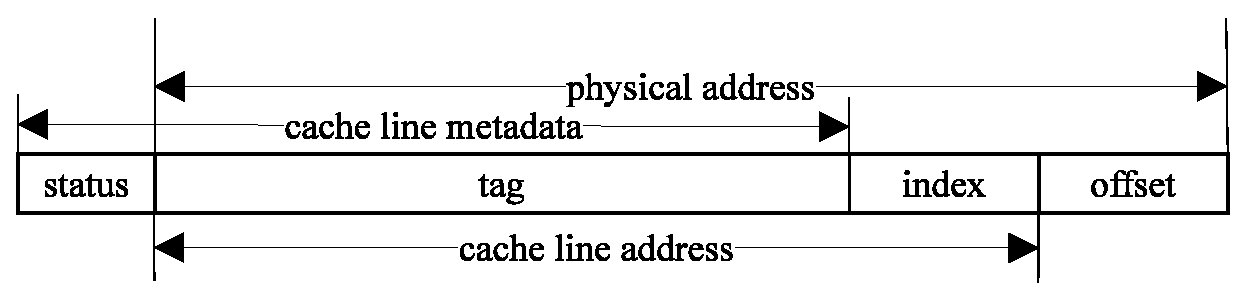
\includegraphics[width=\linewidth]{fig/dinome/tagarray.eps}
\resizebox{0.6\linewidth}{!}{\protect\scriptsize% Graphic for TeX using PGF
% Title: /Users/ziqiaozhou/zzdiss/paper/fig/tagarray_new.dia
% Creator: Dia v0.97.2
% CreationDate: Thu Jun 18 03:05:38 2020
% For: ziqiao
% \usepackage{tikz}
% The following commands are not supported in PSTricks at present
% We define them conditionally, so when they are implemented,
% this pgf file will use them.
\ifx\du\undefined
  \newlength{\du}
\fi
\setlength{\du}{15\unitlength}
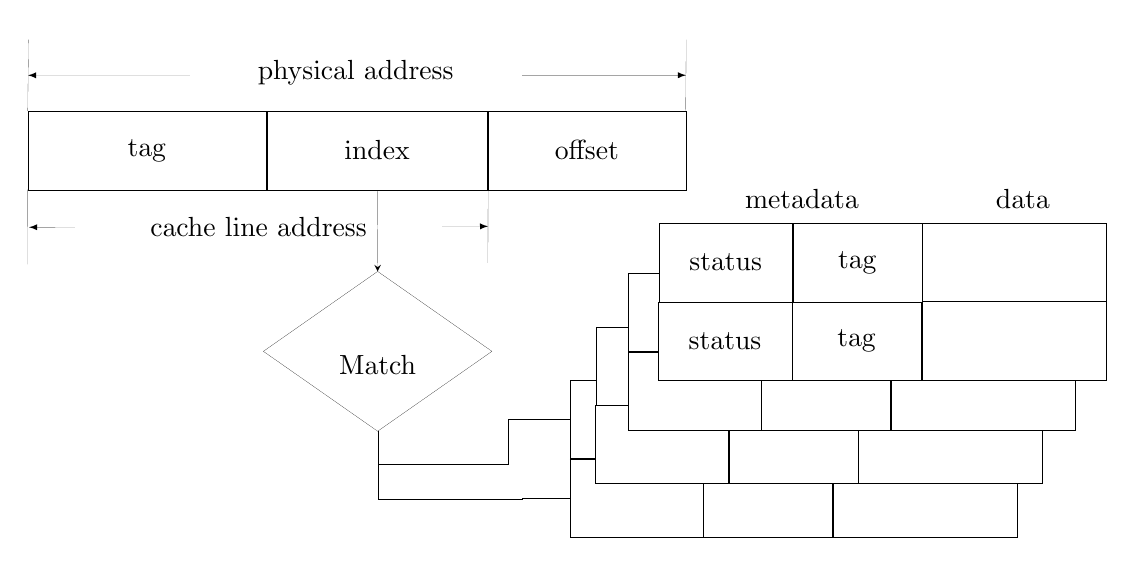
\begin{tikzpicture}
\pgftransformxscale{1.000000}
\pgftransformyscale{-1.000000}
\definecolor{dialinecolor}{rgb}{0.000000, 0.000000, 0.000000}
\pgfsetstrokecolor{dialinecolor}
\definecolor{dialinecolor}{rgb}{1.000000, 1.000000, 1.000000}
\pgfsetfillcolor{dialinecolor}
\pgfsetlinewidth{0.100000\du}
\pgfsetdash{{1.000000\du}{1.000000\du}}{0\du}
\pgfsetdash{{0.100000\du}{0.100000\du}}{0\du}
\pgfsetmiterjoin
\definecolor{dialinecolor}{rgb}{1.000000, 1.000000, 1.000000}
\pgfsetfillcolor{dialinecolor}
\fill (27.608400\du,2.495308\du)--(27.608400\du,3.495308\du)--(29.941231\du,3.495308\du)--(29.941231\du,2.495308\du)--cycle;
\definecolor{dialinecolor}{rgb}{0.000000, 0.000000, 0.000000}
\pgfsetstrokecolor{dialinecolor}
\draw (27.608400\du,2.495308\du)--(27.608400\du,3.495308\du)--(29.941231\du,3.495308\du)--(29.941231\du,2.495308\du)--cycle;
\pgfsetlinewidth{0.100000\du}
\pgfsetdash{{0.100000\du}{0.100000\du}}{0\du}
\pgfsetdash{{0.100000\du}{0.100000\du}}{0\du}
\pgfsetmiterjoin
\definecolor{dialinecolor}{rgb}{1.000000, 1.000000, 1.000000}
\pgfsetfillcolor{dialinecolor}
\fill (27.609100\du,3.482218\du)--(27.609100\du,4.482218\du)--(29.941165\du,4.482218\du)--(29.941165\du,3.482218\du)--cycle;
\definecolor{dialinecolor}{rgb}{0.000000, 0.000000, 0.000000}
\pgfsetstrokecolor{dialinecolor}
\draw (27.609100\du,3.482218\du)--(27.609100\du,4.482218\du)--(29.941165\du,4.482218\du)--(29.941165\du,3.482218\du)--cycle;
\pgfsetlinewidth{0.100000\du}
\pgfsetdash{{0.100000\du}{0.100000\du}}{0\du}
\pgfsetdash{{0.100000\du}{0.100000\du}}{0\du}
\pgfsetmiterjoin
\definecolor{dialinecolor}{rgb}{1.000000, 1.000000, 1.000000}
\pgfsetfillcolor{dialinecolor}
\fill (25.970500\du,2.496208\du)--(25.970500\du,3.488975\du)--(27.605876\du,3.488975\du)--(27.605876\du,2.496208\du)--cycle;
\definecolor{dialinecolor}{rgb}{0.000000, 0.000000, 0.000000}
\pgfsetstrokecolor{dialinecolor}
\draw (25.970500\du,2.496208\du)--(25.970500\du,3.488975\du)--(27.605876\du,3.488975\du)--(27.605876\du,2.496208\du)--cycle;
\pgfsetlinewidth{0.100000\du}
\pgfsetdash{{0.100000\du}{0.100000\du}}{0\du}
\pgfsetdash{{0.100000\du}{0.100000\du}}{0\du}
\pgfsetmiterjoin
\definecolor{dialinecolor}{rgb}{1.000000, 1.000000, 1.000000}
\pgfsetfillcolor{dialinecolor}
\fill (24.270900\du,2.496208\du)--(24.270900\du,3.488975\du)--(25.963313\du,3.488975\du)--(25.963313\du,2.496208\du)--cycle;
\definecolor{dialinecolor}{rgb}{0.000000, 0.000000, 0.000000}
\pgfsetstrokecolor{dialinecolor}
\draw (24.270900\du,2.496208\du)--(24.270900\du,3.488975\du)--(25.963313\du,3.488975\du)--(25.963313\du,2.496208\du)--cycle;
\pgfsetlinewidth{0.100000\du}
\pgfsetdash{{0.100000\du}{0.100000\du}}{0\du}
\pgfsetdash{{0.100000\du}{0.100000\du}}{0\du}
\pgfsetmiterjoin
\definecolor{dialinecolor}{rgb}{1.000000, 1.000000, 1.000000}
\pgfsetfillcolor{dialinecolor}
\fill (25.962300\du,3.491218\du)--(25.962300\du,4.483985\du)--(27.597676\du,4.483985\du)--(27.597676\du,3.491218\du)--cycle;
\definecolor{dialinecolor}{rgb}{0.000000, 0.000000, 0.000000}
\pgfsetstrokecolor{dialinecolor}
\draw (25.962300\du,3.491218\du)--(25.962300\du,4.483985\du)--(27.597676\du,4.483985\du)--(27.597676\du,3.491218\du)--cycle;
\pgfsetlinewidth{0.100000\du}
\pgfsetdash{{0.100000\du}{0.100000\du}}{0\du}
\pgfsetdash{{0.100000\du}{0.100000\du}}{0\du}
\pgfsetmiterjoin
\definecolor{dialinecolor}{rgb}{1.000000, 1.000000, 1.000000}
\pgfsetfillcolor{dialinecolor}
\fill (24.262700\du,3.491218\du)--(24.262700\du,4.483985\du)--(25.955113\du,4.483985\du)--(25.955113\du,3.491218\du)--cycle;
\definecolor{dialinecolor}{rgb}{0.000000, 0.000000, 0.000000}
\pgfsetstrokecolor{dialinecolor}
\draw (24.262700\du,3.491218\du)--(24.262700\du,4.483985\du)--(25.955113\du,4.483985\du)--(25.955113\du,3.491218\du)--cycle;
\pgfsetlinewidth{0.030000\du}
\pgfsetdash{}{0pt}
\pgfsetdash{}{0pt}
\pgfsetmiterjoin
\definecolor{dialinecolor}{rgb}{1.000000, 1.000000, 1.000000}
\pgfsetfillcolor{dialinecolor}
\fill (27.929900\du,1.816670\du)--(27.929900\du,2.816670\du)--(30.262731\du,2.816670\du)--(30.262731\du,1.816670\du)--cycle;
\definecolor{dialinecolor}{rgb}{0.000000, 0.000000, 0.000000}
\pgfsetstrokecolor{dialinecolor}
\draw (27.929900\du,1.816670\du)--(27.929900\du,2.816670\du)--(30.262731\du,2.816670\du)--(30.262731\du,1.816670\du)--cycle;
\pgfsetlinewidth{0.030000\du}
\pgfsetdash{}{0pt}
\pgfsetdash{}{0pt}
\pgfsetmiterjoin
\definecolor{dialinecolor}{rgb}{1.000000, 1.000000, 1.000000}
\pgfsetfillcolor{dialinecolor}
\fill (27.930600\du,2.803580\du)--(27.930600\du,3.803580\du)--(30.262665\du,3.803580\du)--(30.262665\du,2.803580\du)--cycle;
\definecolor{dialinecolor}{rgb}{0.000000, 0.000000, 0.000000}
\pgfsetstrokecolor{dialinecolor}
\draw (27.930600\du,2.803580\du)--(27.930600\du,3.803580\du)--(30.262665\du,3.803580\du)--(30.262665\du,2.803580\du)--cycle;
\pgfsetlinewidth{0.030000\du}
\pgfsetdash{}{0pt}
\pgfsetdash{}{0pt}
\pgfsetmiterjoin
\definecolor{dialinecolor}{rgb}{1.000000, 1.000000, 1.000000}
\pgfsetfillcolor{dialinecolor}
\fill (26.292000\du,1.817570\du)--(26.292000\du,2.810338\du)--(27.927376\du,2.810338\du)--(27.927376\du,1.817570\du)--cycle;
\definecolor{dialinecolor}{rgb}{0.000000, 0.000000, 0.000000}
\pgfsetstrokecolor{dialinecolor}
\draw (26.292000\du,1.817570\du)--(26.292000\du,2.810338\du)--(27.927376\du,2.810338\du)--(27.927376\du,1.817570\du)--cycle;
\pgfsetlinewidth{0.030000\du}
\pgfsetdash{}{0pt}
\pgfsetdash{}{0pt}
\pgfsetmiterjoin
\definecolor{dialinecolor}{rgb}{1.000000, 1.000000, 1.000000}
\pgfsetfillcolor{dialinecolor}
\fill (24.592400\du,1.817570\du)--(24.592400\du,2.810338\du)--(26.284813\du,2.810338\du)--(26.284813\du,1.817570\du)--cycle;
\definecolor{dialinecolor}{rgb}{0.000000, 0.000000, 0.000000}
\pgfsetstrokecolor{dialinecolor}
\draw (24.592400\du,1.817570\du)--(24.592400\du,2.810338\du)--(26.284813\du,2.810338\du)--(26.284813\du,1.817570\du)--cycle;
\pgfsetlinewidth{0.030000\du}
\pgfsetdash{}{0pt}
\pgfsetdash{}{0pt}
\pgfsetmiterjoin
\definecolor{dialinecolor}{rgb}{1.000000, 1.000000, 1.000000}
\pgfsetfillcolor{dialinecolor}
\fill (26.283800\du,2.812580\du)--(26.283800\du,3.805348\du)--(27.919176\du,3.805348\du)--(27.919176\du,2.812580\du)--cycle;
\definecolor{dialinecolor}{rgb}{0.000000, 0.000000, 0.000000}
\pgfsetstrokecolor{dialinecolor}
\draw (26.283800\du,2.812580\du)--(26.283800\du,3.805348\du)--(27.919176\du,3.805348\du)--(27.919176\du,2.812580\du)--cycle;
\pgfsetlinewidth{0.030000\du}
\pgfsetdash{}{0pt}
\pgfsetdash{}{0pt}
\pgfsetmiterjoin
\definecolor{dialinecolor}{rgb}{1.000000, 1.000000, 1.000000}
\pgfsetfillcolor{dialinecolor}
\fill (24.584200\du,2.812580\du)--(24.584200\du,3.805348\du)--(26.276613\du,3.805348\du)--(26.276613\du,2.812580\du)--cycle;
\definecolor{dialinecolor}{rgb}{0.000000, 0.000000, 0.000000}
\pgfsetstrokecolor{dialinecolor}
\draw (24.584200\du,2.812580\du)--(24.584200\du,3.805348\du)--(26.276613\du,3.805348\du)--(26.276613\du,2.812580\du)--cycle;
\pgfsetlinewidth{0.030000\du}
\pgfsetdash{}{0pt}
\pgfsetdash{}{0pt}
\pgfsetmiterjoin
\definecolor{dialinecolor}{rgb}{1.000000, 1.000000, 1.000000}
\pgfsetfillcolor{dialinecolor}
\fill (28.344400\du,1.133710\du)--(28.344400\du,2.133710\du)--(30.677231\du,2.133710\du)--(30.677231\du,1.133710\du)--cycle;
\definecolor{dialinecolor}{rgb}{0.000000, 0.000000, 0.000000}
\pgfsetstrokecolor{dialinecolor}
\draw (28.344400\du,1.133710\du)--(28.344400\du,2.133710\du)--(30.677231\du,2.133710\du)--(30.677231\du,1.133710\du)--cycle;
\pgfsetlinewidth{0.030000\du}
\pgfsetdash{}{0pt}
\pgfsetdash{}{0pt}
\pgfsetmiterjoin
\definecolor{dialinecolor}{rgb}{1.000000, 1.000000, 1.000000}
\pgfsetfillcolor{dialinecolor}
\fill (28.345100\du,2.120620\du)--(28.345100\du,3.120620\du)--(30.677165\du,3.120620\du)--(30.677165\du,2.120620\du)--cycle;
\definecolor{dialinecolor}{rgb}{0.000000, 0.000000, 0.000000}
\pgfsetstrokecolor{dialinecolor}
\draw (28.345100\du,2.120620\du)--(28.345100\du,3.120620\du)--(30.677165\du,3.120620\du)--(30.677165\du,2.120620\du)--cycle;
\pgfsetlinewidth{0.030000\du}
\pgfsetdash{}{0pt}
\pgfsetdash{}{0pt}
\pgfsetmiterjoin
\definecolor{dialinecolor}{rgb}{1.000000, 1.000000, 1.000000}
\pgfsetfillcolor{dialinecolor}
\fill (26.706500\du,1.134610\du)--(26.706500\du,2.127378\du)--(28.341876\du,2.127378\du)--(28.341876\du,1.134610\du)--cycle;
\definecolor{dialinecolor}{rgb}{0.000000, 0.000000, 0.000000}
\pgfsetstrokecolor{dialinecolor}
\draw (26.706500\du,1.134610\du)--(26.706500\du,2.127378\du)--(28.341876\du,2.127378\du)--(28.341876\du,1.134610\du)--cycle;
\pgfsetlinewidth{0.030000\du}
\pgfsetdash{}{0pt}
\pgfsetdash{}{0pt}
\pgfsetmiterjoin
\definecolor{dialinecolor}{rgb}{1.000000, 1.000000, 1.000000}
\pgfsetfillcolor{dialinecolor}
\fill (25.006900\du,1.134610\du)--(25.006900\du,2.127378\du)--(26.699313\du,2.127378\du)--(26.699313\du,1.134610\du)--cycle;
\definecolor{dialinecolor}{rgb}{0.000000, 0.000000, 0.000000}
\pgfsetstrokecolor{dialinecolor}
\draw (25.006900\du,1.134610\du)--(25.006900\du,2.127378\du)--(26.699313\du,2.127378\du)--(26.699313\du,1.134610\du)--cycle;
\pgfsetlinewidth{0.030000\du}
\pgfsetdash{}{0pt}
\pgfsetdash{}{0pt}
\pgfsetmiterjoin
\definecolor{dialinecolor}{rgb}{1.000000, 1.000000, 1.000000}
\pgfsetfillcolor{dialinecolor}
\fill (26.698300\du,2.129620\du)--(26.698300\du,3.122388\du)--(28.333676\du,3.122388\du)--(28.333676\du,2.129620\du)--cycle;
\definecolor{dialinecolor}{rgb}{0.000000, 0.000000, 0.000000}
\pgfsetstrokecolor{dialinecolor}
\draw (26.698300\du,2.129620\du)--(26.698300\du,3.122388\du)--(28.333676\du,3.122388\du)--(28.333676\du,2.129620\du)--cycle;
\pgfsetlinewidth{0.030000\du}
\pgfsetdash{}{0pt}
\pgfsetdash{}{0pt}
\pgfsetmiterjoin
\definecolor{dialinecolor}{rgb}{1.000000, 1.000000, 1.000000}
\pgfsetfillcolor{dialinecolor}
\fill (24.998700\du,2.129620\du)--(24.998700\du,3.122388\du)--(26.691113\du,3.122388\du)--(26.691113\du,2.129620\du)--cycle;
\definecolor{dialinecolor}{rgb}{0.000000, 0.000000, 0.000000}
\pgfsetstrokecolor{dialinecolor}
\draw (24.998700\du,2.129620\du)--(24.998700\du,3.122388\du)--(26.691113\du,3.122388\du)--(26.691113\du,2.129620\du)--cycle;
\definecolor{dialinecolor}{rgb}{1.000000, 1.000000, 1.000000}
\pgfsetfillcolor{dialinecolor}
\fill (21.823667\du,1.111950\du)--(23.275433\du,2.126726\du)--(21.823667\du,3.141502\du)--(20.371900\du,2.126726\du)--cycle;
\pgfsetlinewidth{0.050000\du}
\pgfsetdash{}{0pt}
\pgfsetdash{}{0pt}
\pgfsetmiterjoin
\definecolor{dialinecolor}{rgb}{0.000000, 0.000000, 0.000000}
\pgfsetstrokecolor{dialinecolor}
\draw (21.823667\du,1.111950\du)--(23.275433\du,2.126726\du)--(21.823667\du,3.141502\du)--(20.371900\du,2.126726\du)--cycle;
% setfont left to latex
\definecolor{dialinecolor}{rgb}{0.000000, 0.000000, 0.000000}
\pgfsetstrokecolor{dialinecolor}
\node at (21.823667\du,2.296726\du){Match};
\pgfsetlinewidth{0.030000\du}
\pgfsetdash{}{0pt}
\pgfsetdash{}{0pt}
\pgfsetbuttcap
{
\definecolor{dialinecolor}{rgb}{0.000000, 0.000000, 0.000000}
\pgfsetfillcolor{dialinecolor}
% was here!!!
\pgfsetarrowsstart{latex}
\pgfsetarrowsend{latex}
\definecolor{dialinecolor}{rgb}{0.000000, 0.000000, 0.000000}
\pgfsetstrokecolor{dialinecolor}
\draw (17.397100\du,0.551166\du)--(23.224850\du,0.539583\du);
}
\definecolor{dialinecolor}{rgb}{1.000000, 1.000000, 1.000000}
\pgfsetfillcolor{dialinecolor}
\fill (17.979700\du,-0.024626\du)--(17.979700\du,0.682874\du)--(22.642200\du,0.682874\du)--(22.642200\du,-0.024626\du)--cycle;
% setfont left to latex
\definecolor{dialinecolor}{rgb}{0.000000, 0.000000, 0.000000}
\pgfsetstrokecolor{dialinecolor}
\node at (20.310950\du,0.545374\du){cache line address};
\pgfsetlinewidth{0.030000\du}
\pgfsetdash{}{0pt}
\pgfsetdash{}{0pt}
\pgfsetbuttcap
{
\definecolor{dialinecolor}{rgb}{0.000000, 0.000000, 0.000000}
\pgfsetfillcolor{dialinecolor}
% was here!!!
\definecolor{dialinecolor}{rgb}{0.000000, 0.000000, 0.000000}
\pgfsetstrokecolor{dialinecolor}
\draw (17.379900\du,0.073392\du)--(17.380700\du,1.023490\du);
}
\pgfsetlinewidth{0.030000\du}
\pgfsetdash{}{0pt}
\pgfsetdash{}{0pt}
\pgfsetbuttcap
{
\definecolor{dialinecolor}{rgb}{0.000000, 0.000000, 0.000000}
\pgfsetfillcolor{dialinecolor}
% was here!!!
\definecolor{dialinecolor}{rgb}{0.000000, 0.000000, 0.000000}
\pgfsetstrokecolor{dialinecolor}
\draw (23.226000\du,0.074327\du)--(23.223700\du,1.004840\du);
}
\pgfsetlinewidth{0.030000\du}
\pgfsetdash{}{0pt}
\pgfsetdash{}{0pt}
\pgfsetbuttcap
{
\definecolor{dialinecolor}{rgb}{0.000000, 0.000000, 0.000000}
\pgfsetfillcolor{dialinecolor}
% was here!!!
\definecolor{dialinecolor}{rgb}{0.000000, 0.000000, 0.000000}
\pgfsetstrokecolor{dialinecolor}
\draw (25.741900\du,-1.833290\du)--(25.735600\du,-0.925673\du);
}
\pgfsetlinewidth{0.030000\du}
\pgfsetdash{}{0pt}
\pgfsetdash{}{0pt}
\pgfsetbuttcap
{
\definecolor{dialinecolor}{rgb}{0.000000, 0.000000, 0.000000}
\pgfsetfillcolor{dialinecolor}
% was here!!!
\definecolor{dialinecolor}{rgb}{0.000000, 0.000000, 0.000000}
\pgfsetstrokecolor{dialinecolor}
\draw (17.389200\du,-1.830420\du)--(17.379900\du,-0.926608\du);
}
\pgfsetlinewidth{0.030000\du}
\pgfsetdash{}{0pt}
\pgfsetdash{}{0pt}
\pgfsetbuttcap
{
\definecolor{dialinecolor}{rgb}{0.000000, 0.000000, 0.000000}
\pgfsetfillcolor{dialinecolor}
% was here!!!
\pgfsetarrowsstart{latex}
\pgfsetarrowsend{latex}
\definecolor{dialinecolor}{rgb}{0.000000, 0.000000, 0.000000}
\pgfsetstrokecolor{dialinecolor}
\draw (17.384550\du,-1.378514\du)--(25.738750\du,-1.379482\du);
}
\definecolor{dialinecolor}{rgb}{1.000000, 1.000000, 1.000000}
\pgfsetfillcolor{dialinecolor}
\fill (19.434400\du,-1.983580\du)--(19.434400\du,-1.276080\du)--(23.654400\du,-1.276080\du)--(23.654400\du,-1.983580\du)--cycle;
% setfont left to latex
\definecolor{dialinecolor}{rgb}{0.000000, 0.000000, 0.000000}
\pgfsetstrokecolor{dialinecolor}
\node at (21.544400\du,-1.413580\du){physical address};
\pgfsetlinewidth{0.080000\du}
\pgfsetdash{}{0pt}
\pgfsetdash{}{0pt}
\pgfsetmiterjoin
\pgfsetbuttcap
{
\definecolor{dialinecolor}{rgb}{0.000000, 0.000000, 0.000000}
\pgfsetfillcolor{dialinecolor}
% was here!!!
{\pgfsetcornersarced{\pgfpoint{0.000000\du}{0.000000\du}}\definecolor{dialinecolor}{rgb}{0.000000, 0.000000, 0.000000}
\pgfsetstrokecolor{dialinecolor}
\draw (21.823667\du,3.141502\du)--(21.823667\du,3.555504\du)--(23.476300\du,3.555504\du)--(23.476300\du,2.992591\du)--(24.270900\du,2.992591\du);
}}
\pgfsetlinewidth{0.080000\du}
\pgfsetdash{}{0pt}
\pgfsetdash{}{0pt}
\pgfsetmiterjoin
\pgfsetbuttcap
{
\definecolor{dialinecolor}{rgb}{0.000000, 0.000000, 0.000000}
\pgfsetfillcolor{dialinecolor}
% was here!!!
{\pgfsetcornersarced{\pgfpoint{0.000000\du}{0.000000\du}}\definecolor{dialinecolor}{rgb}{0.000000, 0.000000, 0.000000}
\pgfsetstrokecolor{dialinecolor}
\draw (21.823667\du,3.141502\du)--(21.823667\du,4.000119\du)--(23.659100\du,4.000119\du)--(23.659100\du,3.987601\du)--(24.262700\du,3.987601\du);
}}
\pgfsetlinewidth{0.080000\du}
\pgfsetdash{}{0pt}
\pgfsetdash{}{0pt}
\pgfsetbuttcap
{
\definecolor{dialinecolor}{rgb}{0.000000, 0.000000, 0.000000}
\pgfsetfillcolor{dialinecolor}
% was here!!!
\pgfsetarrowsend{stealth}
\definecolor{dialinecolor}{rgb}{0.000000, 0.000000, 0.000000}
\pgfsetstrokecolor{dialinecolor}
\draw (21.816800\du,0.073392\du)--(21.823667\du,1.111950\du);
}
\pgfsetlinewidth{0.050000\du}
\pgfsetdash{}{0pt}
\pgfsetdash{}{0pt}
\pgfsetmiterjoin
\definecolor{dialinecolor}{rgb}{1.000000, 1.000000, 1.000000}
\pgfsetfillcolor{dialinecolor}
\fill (17.379900\du,-0.926608\du)--(17.379900\du,0.073392\du)--(20.402119\du,0.073392\du)--(20.402119\du,-0.926608\du)--cycle;
\definecolor{dialinecolor}{rgb}{0.000000, 0.000000, 0.000000}
\pgfsetstrokecolor{dialinecolor}
\draw (17.379900\du,-0.926608\du)--(17.379900\du,0.073392\du)--(20.402119\du,0.073392\du)--(20.402119\du,-0.926608\du)--cycle;
\pgfsetlinewidth{0.050000\du}
\pgfsetdash{}{0pt}
\pgfsetdash{}{0pt}
\pgfsetmiterjoin
\definecolor{dialinecolor}{rgb}{1.000000, 1.000000, 1.000000}
\pgfsetfillcolor{dialinecolor}
\fill (20.417300\du,-0.926608\du)--(20.417300\du,0.073392\du)--(23.216400\du,0.073392\du)--(23.216400\du,-0.926608\du)--cycle;
\definecolor{dialinecolor}{rgb}{0.000000, 0.000000, 0.000000}
\pgfsetstrokecolor{dialinecolor}
\draw (20.417300\du,-0.926608\du)--(20.417300\du,0.073392\du)--(23.216400\du,0.073392\du)--(23.216400\du,-0.926608\du)--cycle;
% setfont left to latex
\definecolor{dialinecolor}{rgb}{0.000000, 0.000000, 0.000000}
\pgfsetstrokecolor{dialinecolor}
\node at (18.891000\du,-0.426608\du){tag};
% setfont left to latex
\definecolor{dialinecolor}{rgb}{0.000000, 0.000000, 0.000000}
\pgfsetstrokecolor{dialinecolor}
\node at (21.816800\du,-0.426608\du){index};
\pgfsetlinewidth{0.050000\du}
\pgfsetdash{}{0pt}
\pgfsetdash{}{0pt}
\pgfsetmiterjoin
\definecolor{dialinecolor}{rgb}{1.000000, 1.000000, 1.000000}
\pgfsetfillcolor{dialinecolor}
\fill (23.226000\du,-0.925673\du)--(23.226000\du,0.074327\du)--(25.735645\du,0.074327\du)--(25.735645\du,-0.925673\du)--cycle;
\definecolor{dialinecolor}{rgb}{0.000000, 0.000000, 0.000000}
\pgfsetstrokecolor{dialinecolor}
\draw (23.226000\du,-0.925673\du)--(23.226000\du,0.074327\du)--(25.735645\du,0.074327\du)--(25.735645\du,-0.925673\du)--cycle;
% setfont left to latex
\definecolor{dialinecolor}{rgb}{0.000000, 0.000000, 0.000000}
\pgfsetstrokecolor{dialinecolor}
\node at (24.480800\du,-0.425673\du){offset};
\pgfsetlinewidth{0.030000\du}
\pgfsetdash{}{0pt}
\pgfsetdash{}{0pt}
\pgfsetmiterjoin
\definecolor{dialinecolor}{rgb}{1.000000, 1.000000, 1.000000}
\pgfsetfillcolor{dialinecolor}
\fill (28.734800\du,0.501120\du)--(28.734800\du,1.501120\du)--(31.067631\du,1.501120\du)--(31.067631\du,0.501120\du)--cycle;
\definecolor{dialinecolor}{rgb}{0.000000, 0.000000, 0.000000}
\pgfsetstrokecolor{dialinecolor}
\draw (28.734800\du,0.501120\du)--(28.734800\du,1.501120\du)--(31.067631\du,1.501120\du)--(31.067631\du,0.501120\du)--cycle;
\pgfsetlinewidth{0.030000\du}
\pgfsetdash{}{0pt}
\pgfsetdash{}{0pt}
\pgfsetmiterjoin
\definecolor{dialinecolor}{rgb}{1.000000, 1.000000, 1.000000}
\pgfsetfillcolor{dialinecolor}
\fill (28.735600\du,1.488020\du)--(28.735600\du,2.488020\du)--(31.067665\du,2.488020\du)--(31.067665\du,1.488020\du)--cycle;
\definecolor{dialinecolor}{rgb}{0.000000, 0.000000, 0.000000}
\pgfsetstrokecolor{dialinecolor}
\draw (28.735600\du,1.488020\du)--(28.735600\du,2.488020\du)--(31.067665\du,2.488020\du)--(31.067665\du,1.488020\du)--cycle;
\pgfsetlinewidth{0.030000\du}
\pgfsetdash{}{0pt}
\pgfsetdash{}{0pt}
\pgfsetmiterjoin
\definecolor{dialinecolor}{rgb}{1.000000, 1.000000, 1.000000}
\pgfsetfillcolor{dialinecolor}
\fill (27.096900\du,0.502020\du)--(27.096900\du,1.494788\du)--(28.732276\du,1.494788\du)--(28.732276\du,0.502020\du)--cycle;
\definecolor{dialinecolor}{rgb}{0.000000, 0.000000, 0.000000}
\pgfsetstrokecolor{dialinecolor}
\draw (27.096900\du,0.502020\du)--(27.096900\du,1.494788\du)--(28.732276\du,1.494788\du)--(28.732276\du,0.502020\du)--cycle;
\pgfsetlinewidth{0.030000\du}
\pgfsetdash{}{0pt}
\pgfsetdash{}{0pt}
\pgfsetmiterjoin
\definecolor{dialinecolor}{rgb}{1.000000, 1.000000, 1.000000}
\pgfsetfillcolor{dialinecolor}
\fill (25.397300\du,0.502020\du)--(25.397300\du,1.494788\du)--(27.089713\du,1.494788\du)--(27.089713\du,0.502020\du)--cycle;
\definecolor{dialinecolor}{rgb}{0.000000, 0.000000, 0.000000}
\pgfsetstrokecolor{dialinecolor}
\draw (25.397300\du,0.502020\du)--(25.397300\du,1.494788\du)--(27.089713\du,1.494788\du)--(27.089713\du,0.502020\du)--cycle;
% setfont left to latex
\definecolor{dialinecolor}{rgb}{0.000000, 0.000000, 0.000000}
\pgfsetstrokecolor{dialinecolor}
\node at (26.243500\du,0.998404\du){status};
% setfont left to latex
\definecolor{dialinecolor}{rgb}{0.000000, 0.000000, 0.000000}
\pgfsetstrokecolor{dialinecolor}
\node at (27.914600\du,0.998404\du){tag};
\pgfsetlinewidth{0.030000\du}
\pgfsetdash{}{0pt}
\pgfsetdash{}{0pt}
\pgfsetmiterjoin
\definecolor{dialinecolor}{rgb}{1.000000, 1.000000, 1.000000}
\pgfsetfillcolor{dialinecolor}
\fill (27.088700\du,1.497030\du)--(27.088700\du,2.489798\du)--(28.724076\du,2.489798\du)--(28.724076\du,1.497030\du)--cycle;
\definecolor{dialinecolor}{rgb}{0.000000, 0.000000, 0.000000}
\pgfsetstrokecolor{dialinecolor}
\draw (27.088700\du,1.497030\du)--(27.088700\du,2.489798\du)--(28.724076\du,2.489798\du)--(28.724076\du,1.497030\du)--cycle;
\pgfsetlinewidth{0.030000\du}
\pgfsetdash{}{0pt}
\pgfsetdash{}{0pt}
\pgfsetmiterjoin
\definecolor{dialinecolor}{rgb}{1.000000, 1.000000, 1.000000}
\pgfsetfillcolor{dialinecolor}
\fill (25.389100\du,1.497030\du)--(25.389100\du,2.489798\du)--(27.081513\du,2.489798\du)--(27.081513\du,1.497030\du)--cycle;
\definecolor{dialinecolor}{rgb}{0.000000, 0.000000, 0.000000}
\pgfsetstrokecolor{dialinecolor}
\draw (25.389100\du,1.497030\du)--(25.389100\du,2.489798\du)--(27.081513\du,2.489798\du)--(27.081513\du,1.497030\du)--cycle;
% setfont left to latex
\definecolor{dialinecolor}{rgb}{0.000000, 0.000000, 0.000000}
\pgfsetstrokecolor{dialinecolor}
\node at (26.235300\du,1.993410\du){status};
% setfont left to latex
\definecolor{dialinecolor}{rgb}{0.000000, 0.000000, 0.000000}
\pgfsetstrokecolor{dialinecolor}
\node at (27.906400\du,1.993410\du){tag};
\definecolor{dialinecolor}{rgb}{1.000000, 1.000000, 1.000000}
\pgfsetfillcolor{dialinecolor}
\fill (26.057200\du,-0.377595\du)--(26.057200\du,0.329905\du)--(28.367200\du,0.329905\du)--(28.367200\du,-0.377595\du)--cycle;
% setfont left to latex
\definecolor{dialinecolor}{rgb}{0.000000, 0.000000, 0.000000}
\pgfsetstrokecolor{dialinecolor}
\node at (27.212200\du,0.192405\du){metadata};
\definecolor{dialinecolor}{rgb}{1.000000, 1.000000, 1.000000}
\pgfsetfillcolor{dialinecolor}
\fill (29.483450\du,-0.374605\du)--(29.483450\du,0.332895\du)--(30.550950\du,0.332895\du)--(30.550950\du,-0.374605\du)--cycle;
% setfont left to latex
\definecolor{dialinecolor}{rgb}{0.000000, 0.000000, 0.000000}
\pgfsetstrokecolor{dialinecolor}
\node at (30.017200\du,0.195395\du){data};
\end{tikzpicture}
}
\caption{Way-associated cache in \boom}
\label{fig:tagarray}
\end{figure}

\boom provides a configurable L1 cache module using a random
replacement policy, where its memory-to-cache mapping is shown in
\figref{fig:tagarray}.  In the following experiments, we used
pocket-size hardware modules to replace the modules in the \boom
v2.2.3 configuration. Although the system we evaluated is configured
to be much smaller than an actual system, it preserves all of the
original functionality; analyzing artificially small but otherwise
faithful configurations of a system is not uncommon on model checking,
for example (e.g.,~\cite{ball2004slam,pnueli2002small}).
Specifically, we set the cache line size to $\blockBytes = 64\bytes$
and the total L1 data cache size to $1\kilobytes$ (16 cache lines in
total).  We then varied the cache ways \cacheLineNmbr and sets
\cachesetNmbr (i.e., subject to $\cacheLineNmbr \times \cachesetNmbr =
16$) in \secref{dinome:sec:exp:cache} but used a fixed setting $\cachesetNmbr
= 2$, $\cachesetNmbr = 8$ for other evaluations.  For the main memory,
we set the memory size to $4\kilobytes$ and thus a memory address is
only 12~bits. For evaluation purposes, we used the upper half of the
memory address space as instruction memory and the lower half as data
memory. To simplify the following analysis, we removed the \gls{PTW}
module and assumed virtual addresses were the same as physical
addresses.  For the instruction fetch, we set the fetch width to 4 and
configured the L1 instruction cache to a $1\kilobytes$, $8$-set,
$2$-way cache with a customized prefetching module that preloaded the
software workload at the first cycle.

One feature of \boom is that it supports speculative execution, with
which we will experiment in \secref{dinome:sec:exp:spectre}.  Speculative
execution leverages a \textit{branch predictor}, for which we used the
GShare branch predictor.  The logical structure of GShare is shown in
\figref{fig:gshare}. When a prediction request arrives for a branch
instruction, the GShare predictor derives a value \bpdIdx from the
certain bits (denoted `idx' in \figref{fig:gshare}) in the instruction
address and an instruction history register and then uses \bpdIdx to
index into a table to which we refer as `bpd'.  Each entry of the
`bpd' table includes a label called `CFI' and a 2-bit `state', of
which one bit indicates whether the entry holds a strong or weak
prediction and the other bit holds that prediction (i.e., whether the
branch will be taken or not).  If the \bpdCFI{\bpdIdx} value matches
the `CFI' portion of the instruction address, then the predictor uses
the \bpdState{\bpdIdx} value to make a branch prediction.  The GShare
predictor will globally tune entries based on executions in any user's
domain. Thus, an attacker can easily affect the `bpd' table before
victim's execution, and so we include `bpd' in \ACIKeys. In our
evaluation, we fix the number of `bpd' entries to 4 so that only 2
bits in the instruction address are used as `idx' while another 2 bits
(=$\log_2$(fetch width)) are used as its `CFI' label.

In the following case studies, we added the `bpd' table in the GShare
module to \ACIKeys and registers in the L1 data cache module including
the cache metadata, the replacement state (i.e., the \gls{LFSR} for
the random replacement policy), and the memory-to-cache mapping (if
using a nonfixed mapping) to \AIIKeys.

%Then the
%evaluation will focus on noninterference when an attacker can use
%\ACIFn{}(\loadVar)[\blockIdx]) to choose whether load or flush a memory
%block for his \nControlledMem controllable blocks and observe
%\AOOFn{}(\hitsVar{[\blockIdx]}) whether a memory block \blockIdx is in
%cache.
\begin{figure}[t]
%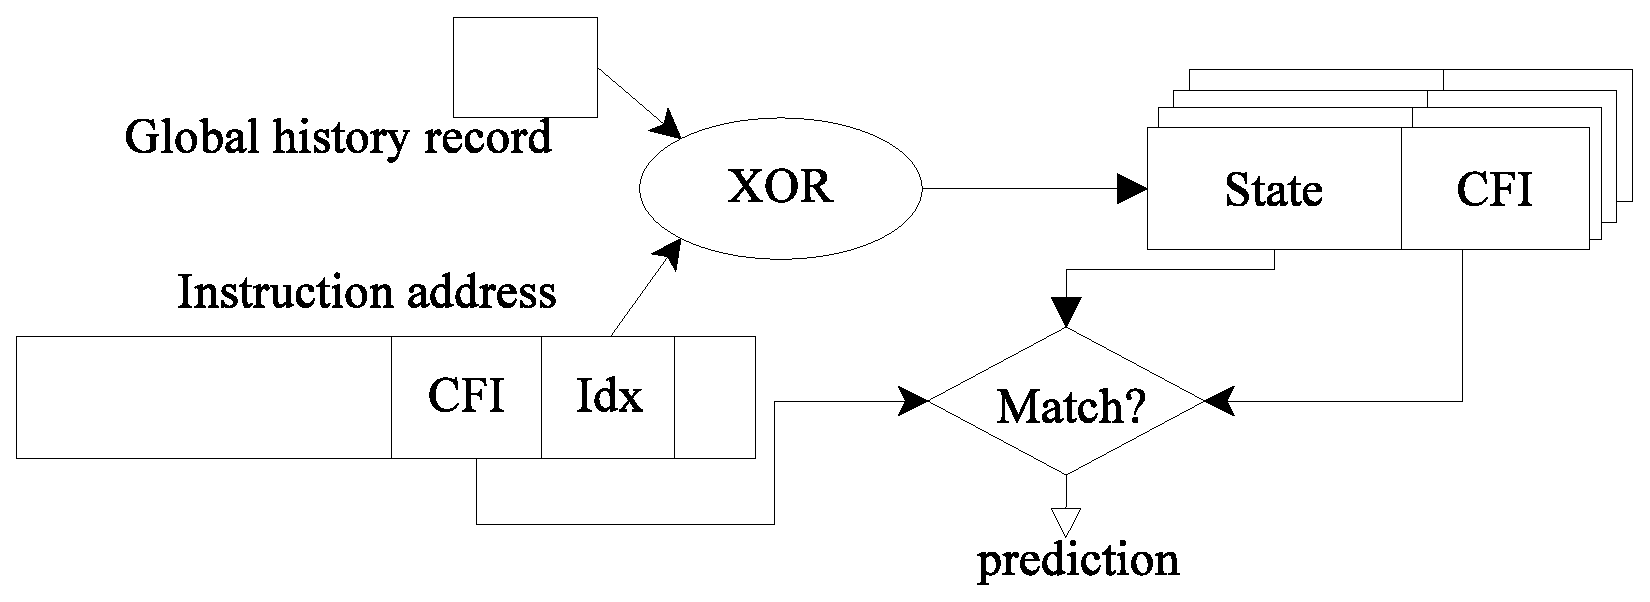
\includegraphics[width=\linewidth]{fig/dinome/gshare.eps}
\centering
\resizebox{0.7\linewidth}{!}{\protect\small% Graphic for TeX using PGF
% Title: /Users/ziqiaozhou/zzdiss/paper/fig/gshare.dia
% Creator: Dia v0.97.2
% CreationDate: Tue Jun 23 13:17:54 2020
% For: ziqiao
% \usepackage{tikz}
% The following commands are not supported in PSTricks at present
% We define them conditionally, so when they are implemented,
% this pgf file will use them.
\ifx\du\undefined
  \newlength{\du}
\fi
\setlength{\du}{11\unitlength}
\begin{tikzpicture}
\pgftransformxscale{1.000000}
\pgftransformyscale{-1.000000}
\definecolor{dialinecolor}{rgb}{0.000000, 0.000000, 0.000000}
\pgfsetstrokecolor{dialinecolor}
\definecolor{dialinecolor}{rgb}{1.000000, 1.000000, 1.000000}
\pgfsetfillcolor{dialinecolor}
\definecolor{dialinecolor}{rgb}{1.000000, 1.000000, 1.000000}
\pgfsetfillcolor{dialinecolor}
\fill (22.990082\du,10.143216\du)--(22.990082\du,11.547796\du)--(26.571524\du,11.547796\du)--(26.571524\du,10.143216\du)--cycle;
\pgfsetlinewidth{0.100000\du}
\pgfsetdash{}{0pt}
\pgfsetdash{}{0pt}
\pgfsetmiterjoin
\definecolor{dialinecolor}{rgb}{0.000000, 0.000000, 0.000000}
\pgfsetstrokecolor{dialinecolor}
\draw (22.990082\du,10.143216\du)--(22.990082\du,11.547796\du)--(26.571524\du,11.547796\du)--(26.571524\du,10.143216\du)--cycle;
% setfont left to latex
\definecolor{dialinecolor}{rgb}{0.000000, 0.000000, 0.000000}
\pgfsetstrokecolor{dialinecolor}
\node at (24.780803\du,11.056617\du){};
\definecolor{dialinecolor}{rgb}{1.000000, 1.000000, 1.000000}
\pgfsetfillcolor{dialinecolor}
\fill (26.559914\du,10.143016\du)--(26.559914\du,11.547796\du)--(29.758062\du,11.547796\du)--(29.758062\du,10.143016\du)--cycle;
\pgfsetlinewidth{0.100000\du}
\pgfsetdash{}{0pt}
\pgfsetdash{}{0pt}
\pgfsetmiterjoin
\definecolor{dialinecolor}{rgb}{0.000000, 0.000000, 0.000000}
\pgfsetstrokecolor{dialinecolor}
\draw (26.559914\du,10.143016\du)--(26.559914\du,11.547796\du)--(29.758062\du,11.547796\du)--(29.758062\du,10.143016\du)--cycle;
% setfont left to latex
\definecolor{dialinecolor}{rgb}{0.000000, 0.000000, 0.000000}
\pgfsetstrokecolor{dialinecolor}
\node at (28.158988\du,11.056517\du){};
\definecolor{dialinecolor}{rgb}{1.000000, 1.000000, 1.000000}
\pgfsetfillcolor{dialinecolor}
\fill (22.572803\du,10.417741\du)--(22.572803\du,11.822322\du)--(26.154245\du,11.822322\du)--(26.154245\du,10.417741\du)--cycle;
\pgfsetlinewidth{0.100000\du}
\pgfsetdash{}{0pt}
\pgfsetdash{}{0pt}
\pgfsetmiterjoin
\definecolor{dialinecolor}{rgb}{0.000000, 0.000000, 0.000000}
\pgfsetstrokecolor{dialinecolor}
\draw (22.572803\du,10.417741\du)--(22.572803\du,11.822322\du)--(26.154245\du,11.822322\du)--(26.154245\du,10.417741\du)--cycle;
% setfont left to latex
\definecolor{dialinecolor}{rgb}{0.000000, 0.000000, 0.000000}
\pgfsetstrokecolor{dialinecolor}
\node at (24.363524\du,11.331143\du){};
\definecolor{dialinecolor}{rgb}{1.000000, 1.000000, 1.000000}
\pgfsetfillcolor{dialinecolor}
\fill (26.142635\du,10.417541\du)--(26.142635\du,11.822322\du)--(29.340784\du,11.822322\du)--(29.340784\du,10.417541\du)--cycle;
\pgfsetlinewidth{0.100000\du}
\pgfsetdash{}{0pt}
\pgfsetdash{}{0pt}
\pgfsetmiterjoin
\definecolor{dialinecolor}{rgb}{0.000000, 0.000000, 0.000000}
\pgfsetstrokecolor{dialinecolor}
\draw (26.142635\du,10.417541\du)--(26.142635\du,11.822322\du)--(29.340784\du,11.822322\du)--(29.340784\du,10.417541\du)--cycle;
% setfont left to latex
\definecolor{dialinecolor}{rgb}{0.000000, 0.000000, 0.000000}
\pgfsetstrokecolor{dialinecolor}
\node at (27.741709\du,11.331043\du){};
\definecolor{dialinecolor}{rgb}{1.000000, 1.000000, 1.000000}
\pgfsetfillcolor{dialinecolor}
\fill (22.170165\du,10.740536\du)--(22.170165\du,12.145117\du)--(25.751607\du,12.145117\du)--(25.751607\du,10.740536\du)--cycle;
\pgfsetlinewidth{0.100000\du}
\pgfsetdash{}{0pt}
\pgfsetdash{}{0pt}
\pgfsetmiterjoin
\definecolor{dialinecolor}{rgb}{0.000000, 0.000000, 0.000000}
\pgfsetstrokecolor{dialinecolor}
\draw (22.170165\du,10.740536\du)--(22.170165\du,12.145117\du)--(25.751607\du,12.145117\du)--(25.751607\du,10.740536\du)--cycle;
% setfont left to latex
\definecolor{dialinecolor}{rgb}{0.000000, 0.000000, 0.000000}
\pgfsetstrokecolor{dialinecolor}
\node at (23.960886\du,11.653937\du){};
\definecolor{dialinecolor}{rgb}{1.000000, 1.000000, 1.000000}
\pgfsetfillcolor{dialinecolor}
\fill (25.739997\du,10.740336\du)--(25.739997\du,12.145117\du)--(28.938146\du,12.145117\du)--(28.938146\du,10.740336\du)--cycle;
\pgfsetlinewidth{0.100000\du}
\pgfsetdash{}{0pt}
\pgfsetdash{}{0pt}
\pgfsetmiterjoin
\definecolor{dialinecolor}{rgb}{0.000000, 0.000000, 0.000000}
\pgfsetstrokecolor{dialinecolor}
\draw (25.739997\du,10.740336\du)--(25.739997\du,12.145117\du)--(28.938146\du,12.145117\du)--(28.938146\du,10.740336\du)--cycle;
% setfont left to latex
\definecolor{dialinecolor}{rgb}{0.000000, 0.000000, 0.000000}
\pgfsetstrokecolor{dialinecolor}
\node at (27.339071\du,11.653837\du){};
% setfont left to latex
\definecolor{dialinecolor}{rgb}{0.000000, 0.000000, 0.000000}
\pgfsetstrokecolor{dialinecolor}
\node at (18.454000\du,9.857800\du){};
\definecolor{dialinecolor}{rgb}{1.000000, 1.000000, 1.000000}
\pgfsetfillcolor{dialinecolor}
\fill (16.107256\du,12.662545\du)--(18.452760\du,13.406780\du)--(16.107256\du,14.151015\du)--(13.761752\du,13.406780\du)--cycle;
\pgfsetlinewidth{0.180000\du}
\pgfsetdash{}{0pt}
\pgfsetdash{}{0pt}
\pgfsetmiterjoin
\definecolor{dialinecolor}{rgb}{0.000000, 0.000000, 0.000000}
\pgfsetstrokecolor{dialinecolor}
\draw (16.107256\du,12.662545\du)--(18.452760\du,13.406780\du)--(16.107256\du,14.151015\du)--(13.761752\du,13.406780\du)--cycle;
% setfont left to latex
\definecolor{dialinecolor}{rgb}{0.000000, 0.000000, 0.000000}
\pgfsetstrokecolor{dialinecolor}
\node at (16.107256\du,13.617892\du){};
% setfont left to latex
\definecolor{dialinecolor}{rgb}{0.000000, 0.000000, 0.000000}
\pgfsetstrokecolor{dialinecolor}
\node at (30.137432\du,16.256434\du){ prediction};
\definecolor{dialinecolor}{rgb}{1.000000, 1.000000, 1.000000}
\pgfsetfillcolor{dialinecolor}
\fill (21.928200\du,11.155200\du)--(21.928200\du,12.559780\du)--(25.509642\du,12.559780\du)--(25.509642\du,11.155200\du)--cycle;
\pgfsetlinewidth{0.100000\du}
\pgfsetdash{}{0pt}
\pgfsetdash{}{0pt}
\pgfsetmiterjoin
\definecolor{dialinecolor}{rgb}{0.000000, 0.000000, 0.000000}
\pgfsetstrokecolor{dialinecolor}
\draw (21.928200\du,11.155200\du)--(21.928200\du,12.559780\du)--(25.509642\du,12.559780\du)--(25.509642\du,11.155200\du)--cycle;
% setfont left to latex
\definecolor{dialinecolor}{rgb}{0.000000, 0.000000, 0.000000}
\pgfsetstrokecolor{dialinecolor}
\node at (23.718921\du,12.068601\du){};
\definecolor{dialinecolor}{rgb}{1.000000, 1.000000, 1.000000}
\pgfsetfillcolor{dialinecolor}
\fill (25.498032\du,11.155000\du)--(25.498032\du,12.559780\du)--(28.913760\du,12.559780\du)--(28.913760\du,11.155000\du)--cycle;
\pgfsetlinewidth{0.100000\du}
\pgfsetdash{}{0pt}
\pgfsetdash{}{0pt}
\pgfsetmiterjoin
\definecolor{dialinecolor}{rgb}{0.000000, 0.000000, 0.000000}
\pgfsetstrokecolor{dialinecolor}
\draw (25.498032\du,11.155000\du)--(25.498032\du,12.559780\du)--(28.913760\du,12.559780\du)--(28.913760\du,11.155000\du)--cycle;
% setfont left to latex
\definecolor{dialinecolor}{rgb}{0.000000, 0.000000, 0.000000}
\pgfsetstrokecolor{dialinecolor}
\node at (27.205896\du,12.068501\du){};
% setfont left to latex
\definecolor{dialinecolor}{rgb}{0.000000, 0.000000, 0.000000}
\pgfsetstrokecolor{dialinecolor}
\node at (23.718921\du,11.857490\du){CFI};
% setfont left to latex
\definecolor{dialinecolor}{rgb}{0.000000, 0.000000, 0.000000}
\pgfsetstrokecolor{dialinecolor}
\node at (27.205896\du,11.857390\du){state};
% setfont left to latex
\definecolor{dialinecolor}{rgb}{0.000000, 0.000000, 0.000000}
\pgfsetstrokecolor{dialinecolor}
\node at (25.457731\du,9.498925\du){GShare $\ACIFn{}(\textrm{`bpd'})$};
% setfont left to latex
\definecolor{dialinecolor}{rgb}{0.000000, 0.000000, 0.000000}
\pgfsetstrokecolor{dialinecolor}
\node at (19.094810\du,11.454096\du){\bpdIdx};
% setfont left to latex
\definecolor{dialinecolor}{rgb}{0.000000, 0.000000, 0.000000}
\pgfsetstrokecolor{dialinecolor}
\node at (25.417008\du,13.227528\du){untaken};
\pgfsetlinewidth{0.180000\du}
\pgfsetdash{}{0pt}
\pgfsetdash{}{0pt}
\pgfsetbuttcap
\pgfsetmiterjoin
\pgfsetlinewidth{0.180000\du}
\pgfsetbuttcap
\pgfsetmiterjoin
\pgfsetdash{}{0pt}
\definecolor{dialinecolor}{rgb}{1.000000, 1.000000, 1.000000}
\pgfsetfillcolor{dialinecolor}
\draw
(24.046019\du,14.540456\du)--(29.065995\du,14.540456\du)--(28.062000\du,15.726772\du)--(25.050014\du,15.726772\du)--(24.046019\du,14.540456\du)--cycle;
%\pgfpathmoveto{\pgfpoint{24.046019\du}{14.540456\du}}
%\pgfpathlineto{\pgfpoint{29.065995\du}{14.540456\du}}
%\pgfpathlineto{\pgfpoint{28.062000\du}{15.726772\du}}
%\pgfpathlineto{\pgfpoint{25.050014\du}{15.726772\du}}
%\pgfpathlineto{\pgfpoint{24.046019\du}{14.540456\du}}
%\pgfusepath{fill}
\definecolor{dialinecolor}{rgb}{0.000000, 0.000000, 0.000000}
\pgfsetstrokecolor{dialinecolor}
\draw
(24.046019\du,14.540456\du)--(29.065995\du,14.540456\du)--(28.062000\du,15.726772\du)--(25.050014\du,15.726772\du)--(24.046019\du,14.540456\du)--cycle;
%\pgfpathmoveto{\pgfpoint{24.046019\du}{14.540456\du}}
%\pgfpathlineto{\pgfpoint{29.065995\du}{14.540456\du}}
%\pgfpathlineto{\pgfpoint{28.062000\du}{15.726772\du}}
%\pgfpathlineto{\pgfpoint{25.050014\du}{15.726772\du}}
%\pgfpathlineto{\pgfpoint{24.046019\du}{14.540456\du}}
%\pgfusepath{stroke}
% setfont left to latex
\definecolor{dialinecolor}{rgb}{0.000000, 0.000000, 0.000000}
\pgfsetstrokecolor{dialinecolor}
\node at (26.556007\du,15.331169\du){};
\pgfsetlinewidth{0.100000\du}
\pgfsetdash{}{0pt}
\pgfsetdash{}{0pt}
\pgfsetmiterjoin
\pgfsetbuttcap
{
\definecolor{dialinecolor}{rgb}{0.000000, 0.000000, 0.000000}
\pgfsetfillcolor{dialinecolor}
% was here!!!
\pgfsetarrowsend{latex}
{\pgfsetcornersarced{\pgfpoint{0.000000\du}{0.000000\du}}\definecolor{dialinecolor}{rgb}{0.000000, 0.000000, 0.000000}
\pgfsetstrokecolor{dialinecolor}
\draw (16.107256\du,14.151015\du)--(16.107256\du,15.133614\du)--(24.548017\du,15.133614\du);
}}
\pgfsetlinewidth{0.100000\du}
\pgfsetdash{}{0pt}
\pgfsetdash{}{0pt}
\pgfsetmiterjoin
\pgfsetbuttcap
{
\definecolor{dialinecolor}{rgb}{0.000000, 0.000000, 0.000000}
\pgfsetfillcolor{dialinecolor}
% was here!!!
\pgfsetarrowsend{latex}
{\pgfsetcornersarced{\pgfpoint{0.000000\du}{0.000000\du}}\definecolor{dialinecolor}{rgb}{0.000000, 0.000000, 0.000000}
\pgfsetstrokecolor{dialinecolor}
\draw (23.718921\du,12.559780\du)--(23.718921\du,13.406780\du)--(18.452760\du,13.406780\du);
}}
% setfont left to latex
\definecolor{dialinecolor}{rgb}{0.000000, 0.000000, 0.000000}
\pgfsetstrokecolor{dialinecolor}
\node at (20.300610\du,14.650734\du){unmatch/match};
\pgfsetlinewidth{0.100000\du}
\pgfsetdash{}{0pt}
\pgfsetdash{}{0pt}
\pgfsetmiterjoin
\pgfsetbuttcap
{
\definecolor{dialinecolor}{rgb}{0.000000, 0.000000, 0.000000}
\pgfsetfillcolor{dialinecolor}
% was here!!!
\pgfsetarrowsend{latex}
{\pgfsetcornersarced{\pgfpoint{0.000000\du}{0.000000\du}}\definecolor{dialinecolor}{rgb}{0.000000, 0.000000, 0.000000}
\pgfsetstrokecolor{dialinecolor}
\draw (26.556007\du,15.726772\du)--(26.556007\du,16.223116\du)--(28.504550\du,16.223116\du);
}}
\pgfsetlinewidth{0.100000\du}
\pgfsetdash{}{0pt}
\pgfsetdash{}{0pt}
\pgfsetbuttcap
{
\definecolor{dialinecolor}{rgb}{0.000000, 0.000000, 0.000000}
\pgfsetfillcolor{dialinecolor}
% was here!!!
\pgfsetarrowsend{latex}
\definecolor{dialinecolor}{rgb}{0.000000, 0.000000, 0.000000}
\pgfsetstrokecolor{dialinecolor}
\draw (25.545504\du,13.566013\du)--(25.554156\du,14.443481\du);
}
\pgfsetlinewidth{0.100000\du}
\pgfsetdash{}{0pt}
\pgfsetdash{}{0pt}
\pgfsetbuttcap
{
\definecolor{dialinecolor}{rgb}{0.000000, 0.000000, 0.000000}
\pgfsetfillcolor{dialinecolor}
% was here!!!
\pgfsetarrowsend{latex}
\definecolor{dialinecolor}{rgb}{0.000000, 0.000000, 0.000000}
\pgfsetstrokecolor{dialinecolor}
\draw (27.205896\du,12.559780\du)--(27.206193\du,14.441649\du);
}
\pgfsetlinewidth{0.100000\du}
\pgfsetdash{}{0pt}
\pgfsetdash{}{0pt}
\pgfsetmiterjoin
\pgfsetbuttcap
{
\definecolor{dialinecolor}{rgb}{0.000000, 0.000000, 0.000000}
\pgfsetfillcolor{dialinecolor}
% was here!!!
\pgfsetarrowsend{latex}
{\pgfsetcornersarced{\pgfpoint{0.000000\du}{0.000000\du}}\definecolor{dialinecolor}{rgb}{0.000000, 0.000000, 0.000000}
\pgfsetstrokecolor{dialinecolor}
\draw (11.988491\du,11.354784\du)--(11.988491\du,13.406780\du)--(13.761752\du,13.406780\du);
}}
\pgfsetlinewidth{0.100000\du}
\pgfsetdash{{\pgflinewidth}{0.200000\du}}{0cm}
\pgfsetdash{{\pgflinewidth}{0.200000\du}}{0cm}
\pgfsetmiterjoin
\pgfsetbuttcap
{
\definecolor{dialinecolor}{rgb}{0.000000, 0.000000, 0.000000}
\pgfsetfillcolor{dialinecolor}
% was here!!!
\pgfsetarrowsend{latex}
{\pgfsetcornersarced{\pgfpoint{0.000000\du}{0.000000\du}}\definecolor{dialinecolor}{rgb}{0.000000, 0.000000, 0.000000}
\pgfsetstrokecolor{dialinecolor}
\draw (14.418341\du,11.354784\du)--(14.418341\du,11.857490\du)--(21.928200\du,11.857490\du);
}}
% setfont left to latex
\definecolor{dialinecolor}{rgb}{0.000000, 0.000000, 0.000000}
\pgfsetstrokecolor{dialinecolor}
\node at (12.785429\du,9.504472\du){Instruction address};
\definecolor{dialinecolor}{rgb}{1.000000, 1.000000, 1.000000}
\pgfsetfillcolor{dialinecolor}
\fill (8.222248\du,9.912439\du)--(8.222248\du,11.354784\du)--(10.715147\du,11.354784\du)--(10.715147\du,9.912439\du)--cycle;
\pgfsetlinewidth{0.100000\du}
\pgfsetdash{}{0pt}
\pgfsetdash{}{0pt}
\pgfsetmiterjoin
\definecolor{dialinecolor}{rgb}{0.000000, 0.000000, 0.000000}
\pgfsetstrokecolor{dialinecolor}
\draw (8.222248\du,9.912439\du)--(8.222248\du,11.354784\du)--(10.715147\du,11.354784\du)--(10.715147\du,9.912439\du)--cycle;
% setfont left to latex
\definecolor{dialinecolor}{rgb}{0.000000, 0.000000, 0.000000}
\pgfsetstrokecolor{dialinecolor}
\node at (9.468698\du,10.844722\du){};
\definecolor{dialinecolor}{rgb}{1.000000, 1.000000, 1.000000}
\pgfsetfillcolor{dialinecolor}
\fill (13.258341\du,9.912439\du)--(13.258341\du,11.354784\du)--(15.578341\du,11.354784\du)--(15.578341\du,9.912439\du)--cycle;
\pgfsetlinewidth{0.100000\du}
\pgfsetdash{}{0pt}
\pgfsetdash{}{0pt}
\pgfsetmiterjoin
\definecolor{dialinecolor}{rgb}{0.000000, 0.000000, 0.000000}
\pgfsetstrokecolor{dialinecolor}
\draw (13.258341\du,9.912439\du)--(13.258341\du,11.354784\du)--(15.578341\du,11.354784\du)--(15.578341\du,9.912439\du)--cycle;
% setfont left to latex
\definecolor{dialinecolor}{rgb}{0.000000, 0.000000, 0.000000}
\pgfsetstrokecolor{dialinecolor}
\node at (14.418341\du,10.844722\du){};
\definecolor{dialinecolor}{rgb}{1.000000, 1.000000, 1.000000}
\pgfsetfillcolor{dialinecolor}
\fill (15.509641\du,9.912439\du)--(15.509641\du,11.354784\du)--(16.872901\du,11.354784\du)--(16.872901\du,9.912439\du)--cycle;
\pgfsetlinewidth{0.100000\du}
\pgfsetdash{}{0pt}
\pgfsetdash{}{0pt}
\pgfsetmiterjoin
\definecolor{dialinecolor}{rgb}{0.000000, 0.000000, 0.000000}
\pgfsetstrokecolor{dialinecolor}
\draw (15.509641\du,9.912439\du)--(15.509641\du,11.354784\du)--(16.872901\du,11.354784\du)--(16.872901\du,9.912439\du)--cycle;
% setfont left to latex
\definecolor{dialinecolor}{rgb}{0.000000, 0.000000, 0.000000}
\pgfsetstrokecolor{dialinecolor}
\node at (16.191271\du,10.844722\du){};
\definecolor{dialinecolor}{rgb}{1.000000, 1.000000, 1.000000}
\pgfsetfillcolor{dialinecolor}
\fill (10.719741\du,9.914039\du)--(10.719741\du,11.354784\du)--(13.257241\du,11.354784\du)--(13.257241\du,9.914039\du)--cycle;
\pgfsetlinewidth{0.100000\du}
\pgfsetdash{}{0pt}
\pgfsetdash{}{0pt}
\pgfsetmiterjoin
\definecolor{dialinecolor}{rgb}{0.000000, 0.000000, 0.000000}
\pgfsetstrokecolor{dialinecolor}
\draw (10.719741\du,9.914039\du)--(10.719741\du,11.354784\du)--(13.257241\du,11.354784\du)--(13.257241\du,9.914039\du)--cycle;
% setfont left to latex
\definecolor{dialinecolor}{rgb}{0.000000, 0.000000, 0.000000}
\pgfsetstrokecolor{dialinecolor}
\node at (11.988491\du,10.845522\du){};
% setfont left to latex
\definecolor{dialinecolor}{rgb}{0.000000, 0.000000, 0.000000}
\pgfsetstrokecolor{dialinecolor}
\node at (11.988491\du,10.634411\du){CFI};
% setfont left to latex
\definecolor{dialinecolor}{rgb}{0.000000, 0.000000, 0.000000}
\pgfsetstrokecolor{dialinecolor}
\node at (14.418341\du,10.633611\du){idx};
% setfont left to latex
\definecolor{dialinecolor}{rgb}{0.000000, 0.000000, 0.000000}
\pgfsetstrokecolor{dialinecolor}
\node at (25.545504\du,15.026702\du){0};
% setfont left to latex
\definecolor{dialinecolor}{rgb}{0.000000, 0.000000, 0.000000}
\pgfsetstrokecolor{dialinecolor}
\node at (27.236388\du,15.026702\du){1};
\end{tikzpicture}
}
\caption{Logical architecture for GShare branch predictor}
\label{fig:gshare}
\end{figure}

\subsection{Logically modeling cache states}

The most common cache-based side-channel attacks are \primeprobe,
\flushreload, and their variants (e.g.,
see~\cite{zhang2012cross,yarom2014flush}).  In a \primeprobe attack,
the attacker loads memory blocks to fill (\Prime) cache sets, permits
the victim computation to run for a \primeprobe interval, and then
reads (\Probe{s}) these same blocks to determine which were evicted by
the victim computation during the \primeprobe interval.  In a
\flushreload attack, the attacker \Flush{es} a shared-memory block
from cache and then, after a \flushreload interval, accesses
(\Reload{s}) the block to determine whether the block was brought
back into the cache by the victim computation.

To model these attacks in our framework, it is necessary to model the
effects on the cache of the phases before victim execution (the \Prime
and \Flush steps) and to define \AOOFn{} to include the results of the
phases after victim execution (the \Probe and \Reload steps).  To do
so, we assume that the adversary has access to memory blocks
\block{1}, \block{2}, $\ldots$, \block{\blockNmbr} aligned to cache
lines, and we define the RISC-V assembly routine \accessProc by which
the adversary can access the block with index $\blockIdx =
\ACIFnAccess{}(\blockIdxVar)$ and empty \SecFnAccess{}:
\begin{center}
\begin{minipage}{0.6\columnwidth}
\begin{tabbing}
\accessProc(\ACIFnAccess{}, \AIIFnAccess{},  \SecFnAccess{}) \\
** \= ** \= \kill
\> \texttt{li s0, 0x2000000}\\ 
\> \texttt{add s1, s0, \blockIdx} \\
\> \texttt{sll s1, s1, 6}\\
\> \texttt{lbu a2, 0(s1)}
\end{tabbing}
\end{minipage}
\end{center}
Starting from hardware state \HwFnAccess{\blockIdx}{0}
($=~\AIIFnAccess{}$) that is completely symbolic, we generate the
per-cycle logical postcondition
$\TmpTransConstraints{\accessProc}(\HwFnAccess{\blockIdx}{\cycle-1},
\HwFnAccess{\blockIdx}{\cycle})$ for each $0 < \cycle \le
\ncyclesAccess$ as in \secref{dinome:sec:impl:logic}, where we empirically
choose $\ncyclesAccess = 45$.

We use these postconditions in two ways.  First, we use them to
extract a constraint
$\glueConstraints{}{}(\langle\HwFn{}{\cycle}\rangle_{\cycle=1}^{\ncycles},
\AOOFn{})$ that defines the attacker's observations \AOOFn{} in terms
of the hardware states
$\langle\HwFn{}{\cycle}\rangle_{\cycle=1}^{\ncycles}$ induced by the
execution (see~\eqnref{eqn:build-postcondition}). A naive attempt to
do so would be to simply include in \AOOFn{} the metadata for each
cache line at every step of the execution.  However, this would grant
too much power to an attacker, who should not be given access to the
tag values and the exact locations of blocks inside a set.  Instead,
we permit only a weaker attacker (cf., abstract
noninterference~\cite{giacobazzi2004abstract}) by defining the
constraint
$\glueConstraints{}{}(\langle\HwFn{}{\cycle}\rangle_{\cycle=1}^{\ncycles},\AOOFn{})$
that represents the view of cache hits and misses immediately
observable by the adversary, by:
\begin{align*}
  \AOOFn{}(\hitVar)[\blockIdx] = &
  \left(\begin{array}{ll}
    (\HwFnAccess{\blockIdx}{0} = \HwFn{}{\ncycles}) \wedge \left(\bigwedge_{\cycle
  = 1}^{\ncyclesAccess}
\TmpTransConstraints{\accessProc}(\HwFnAccess{\blockIdx}{\cycle-1},
\HwFnAccess{\blockIdx}{\cycle})\right) \\
\wedge~\hfill\left(1 - \bigvee_{\cycle = 1}^{\ncyclesAccess}
\cachemiss(\HwFnAccess{\blockIdx}{\cycle}, \block{\blockIdx})\right)
\end{array}\right)
\end{align*}
for $\blockIdx = \ACIFnAccess{}(\blockIdxVar)$.  Here, \cachemiss is a
\boom-defined Verilog code snippet that, intuitively, checks a set of
cache lines where \block{\blockIdx} might reside and returns $1$ (in a
register called \hitRegisterVar) if none of those cache lines has a
valid tag matched with \block{\blockIdx} (and returns $0$ otherwise).
In this way, we characterize the procedure \accessProc using a logical
postcondition without manually modeling \cachemiss.

Second, we permit the attacker to control which of its blocks are
loaded into the cache before the victim runs.  Specifically, the
predicate $\HwPostcondition{\proc}{0}(\ACIFn{}, \AIIFn{}, \SecFn{},
\HwFn{}{0})$ that controls the initial hardware state from which the
victim executes is modified to constrain which of the attacker's
blocks are present in cache, as communicated through a reserved
variable $\loadVar \in \ACIKeys$, for which the
$\ACIFn{}(\loadVar)$ is a bit vector of length \blockNmbr.  That is,
attacker block \block{\blockIdx} should be loaded before the victim
runs if and only if $\ACIFn{}(\loadVar)[\blockIdx] = 1$.  To effect
this in the $\HwPostcondition{\proc}{0}(\ACIFn{},
\AIIFn{}, \SecFn{}, \HwFn{}{0})$, we construct
$\HwPostcondition{\proc}{0}(\ACIFn{}, \AIIFn{}, \SecFn{}, \HwFn{}{0})$
to include
\begin{align*}
  \ACIFn{}(\loadVar)[\blockIdx] = &
  \left(\!\!\!\begin{array}{ll}
    (\HwFnAccess{\blockIdx}{0} = \HwFn{}{0}) \wedge \left(\bigwedge_{\cycle
  = 1}^{\ncyclesAccess}
\TmpTransConstraints{\accessProc}(\HwFnAccess{\blockIdx}{\cycle-1},
\HwFnAccess{\blockIdx}{\cycle})\right) \\
\wedge~\hfill\left(1 - \bigvee_{\cycle = 1}^{\ncyclesAccess}
\cachemiss(\HwFnAccess{\blockIdx}{\cycle}, \block{\blockIdx})\right)
\end{array}\!\!\!\right)
\end{align*}
Of course, we rename variables to ensure no conflicts between copies
of \HwFnAccess{\blockIdx}{\cycle} included within the
$\ACIFn{}(\loadVar)[\blockIdx]$ and $\AOOFn{}(\hitVar)[\blockIdx]$
constraints.

For an attacker, it is sufficient to control the cache using
$\blockNmbr=16$ blocks as the L1 data cache consists of only 16
cache lines in our experiments.

\subsection{Cache-based side channels}
\label{dinome:sec:exp:cache}

In this section, we evaluate cache-based side channels under different
memory isolation and cache configurations.

\subsubsection{Without shared memory}
\label{dinome:sec:exp:cache:normal:unshared}
\begin{figure}
\begin{subfigure}[t]{0.495\linewidth}
\resizebox{\linewidth}{!}{\protect\small\input{fig/dinome/normalcache/normalunshared.tex}}
\caption{Symbolic $\ACIFn{}(\loadVar)$ \label{fig:normalcache:jaccard:unsharedsymload} }
\end{subfigure}%
\begin{subfigure}[t]{0.495\linewidth}
\resizebox{\linewidth}{!}{\protect\small\input{fig/dinome/normalcache/normalprimeprobe.tex}}
\caption{$\forall \blockIdx: \ACIFn{}(\loadVar)[\blockIdx] = 1$ }
\label{fig:normalcache:jaccard:prime}
\end{subfigure}%
\caption{\JaccardRand{\secretsSetSize} for \primeprobe attacks}
\label{fig:normalcache:jaccard:unshared}
\end{figure}
\setlength{\tabcolsep}{0.3ex}
\renewcommand{\arraystretch}{1.3}

\iffalse
\begin{table}
\caption{An rule for \interferenceSet{} in a 2-way 8-set cache w/o shared memory
 \label{tab:s8w2:unshared}}
\vspace{-1ex}
%(depth=8, ntree=64)
\scriptsize{
\begingroup
\everymath{\scriptstyle}
\footnotesize
%your equation
\begin{tabular}{m{\colR}m{\colRule}m{\colPrecision}m{\colRecall}}
\toprule
 & Interference Rule (\interferenceRule{}) & Precision & Recall \\
\midrule
$\interferenceRule{0}$&$\SecFn{}(\secretVar)[2]\ge 1 \wedge
\SecFn{}(\secretVar)[1]< 1 \wedge \SecFn{}(\secretVar)[0]\ge 1 \wedge
\SecFnAlt{}(\secretVar)[1]\ge 1 \wedge \ACIFn{}(\loadVar)[5]\ge 1
\wedge \ACIFn{}(\loadVar)[13]\ge 1$&1.00&0.04\\
\if0
$\interferenceRule{1}$&$\diffFeature{0}\ge 1 \wedge
\SecFn{}(\secretVar)[2]< 1 \wedge \SecFn{}(\secretVar)[1]\ge 1 \wedge
\SecFn{}(\secretVar)[0]\ge 1 \wedge \ACIFn{}(\loadVar)[3]\ge 1 \wedge
\ACIFn{}(\loadVar)[11]\ge 1$&1.00&0.04\\
$\interferenceRule{2}$&$\SecFn{}(\secretVar)\ge 2 \wedge
\SecFnAlt{}(\text{`secret})\ge 9 \wedge \SecFnAlt{}(\text{`secret})< 10
\wedge \ACIFn{}(\loadVar)[9]\ge 1 \wedge \ACIFn{}(\loadVar)[1]\ge
1$&1.00&0.03\\ $\interferenceRule{3}$&$\SecFn{}(\secretVar)\ge 3
\wedge \SecFnAlt{}(\text{`secret})\ge 10 \wedge
\SecFnAlt{}(\text{`secret})< 11 \wedge \ACIFn{}(\loadVar)[2]\ge 1
\wedge \ACIFn{}(\loadVar)[10]\ge 1$&1.00&0.03\\
$\interferenceRule{4}$&$\SecFn{}(\secretVar)\ge 4 \wedge
\SecFnAlt{}(\text{`secret})\ge 11 \wedge \SecFnAlt{}(\secretVar)[2]< 1
\wedge \ACIFn{}(\loadVar)[3]\ge 1 \wedge \ACIFn{}(\loadVar)[11]\ge
1$&1.00&0.03\\ $\interferenceRule{5}$&$\SecFn{}(\secretVar)[0]\ge 1
\wedge \SecFnAlt{}(\text{`secret})< 1 \wedge \ACIFn{}(\loadVar)[8]\ge 1
\wedge \ACIFn{}(\loadVar)[0]\ge 1$&1.00&0.02\\
\fi
\bottomrule
\end{tabular}
\endgroup
}
\vspace{1.5ex}
\caption{Rules for \noninterferenceSet{} for 2-way 8-set cache w/o
memory sharing
\vspace{-1ex}
\label{tab:s8w2:unshared:noninterference}}
\scriptsize{
\begingroup
\everymath{\scriptstyle}
\footnotesize
%your equation
\begin{tabular}{m{\colR}m{\colRule}m{\colPrecision}m{\colRecall}}
\toprule
 & Noninterference rule (\noninterferenceRule{}) & Precision & Recall \\
\midrule
$\noninterferenceRule{0}$&$\diffFeature{2}< 1 \wedge \diffFeature{1}< 1 \wedge \diffFeature{0}< 1$&1.00&0.11\\
\if
$\interferenceRule{1}$&$\SecFn{}(\secretVar)[2]\ge 1 \wedge
\SecFn{}(\secretVar)[0]\ge 1 \wedge \SecFnAlt{}(\secretVar)[2]\ge 1
\wedge \SecFnAlt{}(\secretVar)[0]\ge 1 \wedge \ACIFn{}(\loadVar)[15]< 1 \wedge \ACIFn{}(\loadVar)[13]< 1$&1.00&0.02\\
$\interferenceRule{2}$&$\diffFeature{2}< 1 \wedge \diffFeature{0}< 1 \wedge \SecFn{}(\secretVar)[2]\ge 1 \wedge \SecFn{}(\secretVar)[0]< 1 \wedge \ACIFn{}(\loadVar)[6]< 1 \wedge \ACIFn{}(\loadVar)[12]< 1$&1.00&0.02\\
$\interferenceRule{3}$&$\SecFn{}(\secretVar)[2]\ge 1 \wedge \SecFn{}(\secretVar)[1]\ge 1 \wedge \SecFnAlt{}(\text{`secret})\ge 3 \wedge \SecFnAlt{}(\secretVar)[1]\ge 1 \wedge \ACIFn{}(\loadVar)[7]< 1 \wedge \ACIFn{}(\loadVar)[14]< 1 \wedge \ACIFn{}(\loadVar)[11]< 1$&0.94&0.02\\
$\interferenceRule{4}$&$\diffFeature{2}\ge 1 \wedge \diffFeature{1}\ge 1 \wedge \SecFn{}(\secretVar)\ge 2 \wedge \SecFn{}(\secretVar)< 6 \wedge \ACIFn{}(\loadVar)[5]< 1 \wedge \ACIFn{}(\loadVar)[11]< 1 \wedge \ACIFn{}(\loadVar)[10]< 1$&0.83&0.01\\
$\interferenceRule{5}$&$\diffFeature{2}\ge 1 \wedge \diffFeature{0}\ge 1 \wedge \SecFn{}(\secretVar)\ge 3 \wedge \SecFn{}(\secretVar)[1]\ge 1 \wedge \SecFn{}(\secretVar)< 7 \wedge \ACIFn{}(\loadVar)[6]< 1 \wedge \ACIFn{}(\loadVar)[3]< 1$&0.83&0.01\\
$\interferenceRule{6}$&$\diffFeature{2}< 1 \wedge \SecFn{}(\secretVar)\ge 1 \wedge \SecFn{}(\secretVar)[2]< 1 \wedge \SecFnAlt{}(\secretVar)[1]\ge 1 \wedge \ACIFn{}(\loadVar)[3]< 1 \wedge \ACIFn{}(\loadVar)[2]< 1$&0.83&0.04\\
$\interferenceRule{7}$&$\SecFn{}(\secretVar)[2]< 1 \wedge \SecFn{}(\secretVar)[1]< 1 \wedge \SecFn{}(\secretVar)[0]< 1 \wedge \SecFnAlt{}(\secretVar)[2]\ge 1 \wedge \SecFnAlt{}(\secretVar)[0]\ge 1 \wedge \ACIFn{}(\loadVar)[5]< 1 \wedge \ACIFn{}(\loadVar)[0]< 1$&0.83&0.01\\
$\interferenceRule{8}$&$\SecFn{}(\secretVar)[2]\ge 1 \wedge \SecFn{}(\secretVar)[1]< 1 \wedge \SecFnAlt{}(\text{`secret})\ge 2 \wedge \SecFnAlt{}(\text{`secret})< 6 \wedge \ACIFn{}(\loadVar)[5]< 1 \wedge \ACIFn{}(\loadVar)[4]< 1$&0.80&0.02\\
$\interferenceRule{9}$&$\SecFn{}(\secretVar)[2]\ge 1 \wedge \SecFn{}(\secretVar)[1]< 1 \wedge \ACIFn{}(\loadVar)[4]< 1 \wedge \ACIFn{}(\loadVar)[2]< 1 \wedge \ACIFn{}(\loadVar)[13]< 1$&0.78&0.04\\
\fi
\bottomrule
\end{tabular}
\endgroup
}
\end{table} 
\fi

Here, we target a victim's RISC-V assembly \proc to access a
secret-indexed memory block not shared with the attacker, by setting
the base address in \texttt{s0} to a value \texttt{0x2000010}, in
contrast to the one used in \accessProc.
\begin{align}
\begin{minipage}{0.6\columnwidth}
\begin{tabbing}
\proc(\ACIFn{}, \AIIFn{}, \SecFn{}) \\
** \= ** \= \kill
\> \texttt{li s0, 0x2000010}\\ 
\> \texttt{add s1, s0, $\SecFn{}(\secretVar)$} \\
\> \texttt{sll s1, s1, 6}\\
\> \texttt{lbu a2, 0(s1)}
\end{tabbing}
\end{minipage}
\label{eqn:proc}
\end{align}

We experimented with different numbers of cache sets \cachesetNmbr
including $\cachesetNmbr=1$ (i.e., 1-way, 16-set, fully associative),
$\cachesetNmbr=2$ (i.e., 8-way, 2-set), $\cachesetNmbr=4$ (i.e., 4-way,
4-set), $\cachesetNmbr=8$ (2-way, 8-set), and $\cachesetNmbr=16$ (i.e.,
1-way, 16-set, direct-mapped). As shown in
\figref{fig:normalcache:jaccard:unsharedsymload},
\JaccardRand{\secretsSetSize} increases when the number of sets
increases.  Specifically, there is no leakage
($\JaccardRand{\secretsSetSize} = 0$ for all \secretsSetSize) when
$\cachesetNmbr=1$. Using fewer cache sets, each cache set is shared by
more memory blocks, and so an attacker will have more difficulty
distinguishing one execution from others. When $1 < \cachesetNmbr <
16$, \JaccardRand{\secretsSetSize} decreases as \secretsSetSize grows,
since the attacker can learn only $log_2(\cachesetNmbr)$ bits about the
secret and thus may be unable to distinguish secrets in large sets
(i.e., large \secretsSetSize).

An example \textit{interference} rule for \interferenceSet generated
as described in \secref{dinome:sec:interpret} with the highest precision
(1.00) and a recall $\approx 0.04$ in a 2-way, 8-set cache is:
\begin{align}
  \begin{array}{rrrr}
    & \SecFn{}(\secretVar)[2]\ge 1 & \wedge & \SecFn{}(\secretVar)[1]< 1 \\
    \wedge & \SecFn{}(\secretVar)[0]\ge 1 & \wedge & \SecFnAlt{}(\secretVar)[1]\ge 1 \\
    \wedge & \ACIFn{}(\loadVar)[5]\ge 1   & \wedge & \ACIFn{}(\loadVar)[13]\ge 1
  \end{array}
  \label{eqn:prime-probe-interference}
\end{align}
In this rule, the \SecFn{} and \SecFnAlt{} conjuncts concretize the
least significant 3 bits of $\SecFn{}(\secretVar)$ (i.e.,
$\SecFn{}(\secretVar) \equiv 5 \bmod 8$) and the lowest bit of
$\SecFnAlt{}(\secretVar)$ (i.e., $\SecFnAlt{}(\secretVar) \equiv 0 \bmod 2$). The \ACIFn{} conjuncts are $\ACIFn{}(\loadVar)[5]\ge 1$ and
$\ACIFn{}(\loadVar)[13]\ge 1$; note that $13\equiv 5 \bmod 8$. That
is, an attacker could load all blocks \block{\blockIdx} with
$\blockIdx \equiv 5 \bmod 8$ into cache to distinguish a secret
$\SecFn{}(\secretVar) \equiv 5 \bmod 8$ from $\SecFnAlt{}(\secretVar)
\bmod 8 \in \{0,2,4,6\}$.

Our approach could not directly represent
$\ACIFn{}(\loadVar)[\blockIdx] \equiv \SecFn{}(\secretVar) \bmod
\cachesetNmbr$.  So, the trees in the model split the dataset based on
the cache set index.  As such, there were many other top-ranking rules
similar to \eqnref{eqn:prime-probe-interference}, each focusing on one
residue class of the secret value modulo \cachesetNmbr where
$\cachesetNmbr=8$ and constraining $\ACIFn{}(\loadVar)[\blockIdx] = 1$
for all \blockIdx with that residue class modulo \cachesetNmbr.  Each
such rule works for $\frac{1}{8}$ of \SecFn{}'s domain and
$\frac{1}{2}$ of \SecFnAlt{}'s domain, thus only for
$\frac{1}{8}\times\frac{1}{2}\approx0.06$ of secret pairs. The recall
rate $0.04 < 0.06$ indicates that priming the corresponding cache set
ensures (i.e., precision $=~1.0$) the interference but is not
necessary to cause it.

Analogously, we can generate rules for the \textit{noninterference}
set \noninterferenceSet, as well.  One example with precision 1.0
(i.e., that ensures noninterference) and recall 0.11 constrains the
secret's least-significant 3 bits to be the same for \SecFn{} and
\SecFnAlt{}:
\begin{align}
  \begin{array}{rr}
  & \diffFeature{2}< 1 \\
  \wedge & \diffFeature{1}< 1 \\
  \wedge & \diffFeature{0}< 1
  \end{array}
  \label{eqn:prime-probe-noninterference}
\end{align}
This analysis illustrates that an attacker can easily distinguish
$\SecFn{}(\secretVar)$ and $\SecFnAlt{}(\secretVar)$ when priming a
cache set used by $\SecFn{}(\secretVar)$ or $\SecFnAlt{}(\secretVar)$
but not both.  It is therefore safe to assume that the attacker will
\Prime the cache using all its controlled memory blocks to maximize
the chances for leakage.  The \JaccardRand{ \secretsSetSize} measure
under this specific attack is shown in
\figref{fig:normalcache:jaccard:prime}. The worst case will leak all
of the 4-bit secret when using high-granularity memory-to-cache
mapping, i.e., where $\cachesetNmbr=16$.

\if
For
example, an attacker could partially fill one cache set by only set
$\ACIFn{}(\loadVar)[5]\ge 1$, then he still have some chance to observe
the cache miss caused by the victim with a random replacement policy.
\fi
 
\subsubsection{With shared memory}

\begin{figure}
\begin{subfigure}[t]{0.495\linewidth}
\resizebox{\linewidth}{!}{\protect\small\input{fig/dinome/normalcache/normalshared.tex}}
\caption{Symbolic $\ACIFn{}(\loadVar)$ \label{fig:normalcache:jaccard:sharedsymloads}
}
\end{subfigure}%
\begin{subfigure}[t]{0.495\linewidth}
\resizebox{\linewidth}{!}{\protect\small\input{fig/dinome/normalcache/normalflushreload.tex}}
\caption{$\forall \blockIdx: \ACIFn{}(\loadVar)[\blockIdx] = 0$
  \label{fig:normalcache:jaccard:flushreload}
}
\end{subfigure}% 
\caption{\JaccardRand{\secretsSetSize} for \flushreload attacks}
\end{figure}


\iffalse
\begin{table}
\caption{Selected interference rules when \cachesetNmbr=8 with memory sharing\label{tab:s8w2:shared}.}
\scriptsize{
\begingroup
\everymath{\scriptstyle}
\footnotesize
%your equation
\begin{tabular}{m{\colR}m{\colRule}m{\colPrecision}m{\colRecall}}
\toprule
 & Interference Rule (\interferenceRule{}) & Precision & Recall \\
\midrule
$\interferenceRule{0}$&$\SecFnAlt{}(\secretVar)< 2 \wedge \SecFnAlt{}(\secretVar)\ge 1 \wedge \ACIFn{}(\loadVar)[1]< 1$&1.00&0.04\\
\if 0
$\interferenceRule{1}$&$\SecFn{}(\secretVar)[1]< 1 \wedge \SecFn{}(\secretVar)< 4 \wedge \ACIFn{}(\loadVar)[1]< 1 \wedge \ACIFn{}(\loadVar)[0]< 1$&1.00&0.04\\
$\interferenceRule{2}$&$\SecFnAlt{}(\secretVar)\ge 15 \wedge \ACIFn{}(\loadVar)[15]< 1$&1.00&0.04\\
$\interferenceRule{3}$&$\SecFnAlt{}(\secretVar)\ge 13 \wedge \SecFnAlt{}(\secretVar)[1]\ge 1 \wedge \SecFnAlt{}(\secretVar)[0]\ge 1 \wedge \ACIFn{}(\loadVar)[15]< 1$&1.00&0.04\\
$\interferenceRule{4}$&$\SecFn{}(\secretVar)\ge 12 \wedge \SecFn{}(\secretVar)[1]< 1 \wedge \ACIFn{}(\loadVar)[13]< 1 \wedge \ACIFn{}(\loadVar)[12]< 1$&1.00&0.04\\
$\interferenceRule{5}$&$\SecFn{}(\secretVar)[2]\ge 1 \wedge \SecFn{}(\secretVar)[1]\ge 1 \wedge \SecFn{}(\secretVar)< 7 \wedge \ACIFn{}(\loadVar)[6]< 1$&1.00&0.04\\
$\interferenceRule{6}$&$\SecFn{}(\secretVar)\ge 11 \wedge \SecFn{}(\secretVar)[2]\ge 1 \wedge \SecFn{}(\secretVar)< 13 \wedge \ACIFn{}(\loadVar)[12]< 1$&1.00&0.04\\
$\interferenceRule{7}$&$\SecFnAlt{}(\secretVar)\ge 5 \wedge \SecFnAlt{}(\secretVar)< 7 \wedge \ACIFn{}(\loadVar)[6]< 1 \wedge \ACIFn{}(\loadVar)[5]< 1$&1.00&0.04\\
$\interferenceRule{8}$&$\SecFn{}(\secretVar)\ge 10 \wedge \SecFn{}(\secretVar)[1]< 1 \wedge \SecFn{}(\secretVar)[0]\ge 1 \wedge \ACIFn{}(\loadVar)[13]< 1$&1.00&0.04\\
$\interferenceRule{9}$&$\SecFn{}(\secretVar)[3]\ge 1 \wedge \SecFn{}(\secretVar)[2]\ge 1 \wedge \SecFn{}(\secretVar)[1]< 1 \wedge \SecFn{}(\secretVar)[0]\ge 1 \wedge \ACIFn{}(\loadVar)[13]< 1$&1.00&0.04\\
$\interferenceRule{10}$&$\SecFnAlt{}(\secretVar)\ge 4 \wedge
\SecFnAlt{}(\secretVar)[3]< 1 \wedge
\SecFnAlt{}(\secretVar)[1]\ge 1 \wedge
\SecFnAlt{}(\secretVar)[0]< 1 \wedge \ACIFn{}(\loadVar)[6]<
1$&1.00&0.04\\
\fi
\bottomrule
\end{tabular}
\endgroup
}
\end{table} 
\fi

To evaluate the leakage with memory sharing enabled (i.e., with
\Flush+\Reload attacks), we allow the attacker to control and observe
all memory blocks used by the victim by setting the base to
\texttt{0x2000000} in \proc instead of to \texttt{0x2000010} (see
\eqnref{eqn:proc}).  \figref{fig:normalcache:jaccard:sharedsymloads}
shows the corresponding \JaccardRand{\secretsSetSize}.  The
\JaccardRand{\secretsSetSize} curves are similar and close to 1 for
all settings, indicating that the leakage does not have much
correlation with \cacheLineNmbr.  An example rule for interference
derived using the methodology of \secref{dinome:sec:interpret}, having a
precision of $1.0$ and recall of $\approx 0.04$, is
\begin{align}
  \SecFnAlt{}(\secretVar)< 2 \wedge \SecFnAlt{}(\secretVar)\ge 1 \wedge \ACIFn{}(\loadVar)[1]< 1
  \label{eqn:flush-reload-interference}
\end{align}
That is, if $\SecFnAlt{}(\secretVar)=1$ then $\ACIFn{}(\loadVar)[1]=0$
results in interference.  Indeed, the other top-ranked rules for this
example (not shown) were roughly 32 similar rules, each one setting
$\ACIFn{}(\loadVar)[\blockIdx]=0$ for a specific secret value
$\SecFn{}(\secretVar)=\blockIdx$ or
$\SecFnAlt{}(\secretVar)=\blockIdx$.  The intuition behind these rules
is that an attacker can precisely detect if $\SecFn{}(\secretVar) =
\blockIdx$ by setting $\ACIFn{}(\loadVar)[\blockIdx]=0$ (i.e.,
\Flush{}ing \block{\blockIdx} so he can later \Reload it), and
similarly for $\SecFnAlt{}(\secretVar)$.  Going further, if an
attacker sets $\ACIFn{}(\loadVar)[\blockIdx] = 0$ for all \blockIdx,
he can detect the victim's access to any \block{\blockIdx}, as shown
in \figref{fig:normalcache:jaccard:flushreload} where
$\JaccardRand{\secretsSetSize}=1$ for all \secretsSetSize.

\if0
\subsubsection{Partially shared memory}
\zz{Add it \figref{fig:normal:jaccard:partial} here or not? 8-bit
\SecFn{}(\secretVar) in \proc and \texttt{base=0x2000000}. Then 16/256
memory blocks are shared and 240/256 is unshared.} The interesting
question reflected by this evaluation is when \primeprobe or
\flushreload is the best strategy when the memory is partially
shared. In \figref{fig:normal:jaccard:partial}, we present the
\JaccardRand{\secretsSetSize} when we symbolized the
\ACIFn{}(\loadVar) (denoted by `sym') or applied \primeprobe and
\flushreload. Without a specific attack strategy,
\JaccardRand{\secretsSetSize} is relatively high when
\secretsSetSize is either small enough or large enough. This indicate
that most secret value would be slightly leaked with high chance while
only a portion of secret value would be highly leaked. Under
\primeprobe attack among all cache sets, the
\JaccardRand{\secretsSetSize} decreases with the \secretsSetSize,
indicating that only a limited amount of information about the secret
could be leaked. Under \flushreload attacks among all shared blocks,
\JaccardRand{\secretsSetSize} increases with the \secretsSetSize,
indicating that a secret value would be fully leaked under a limited
chance $\leakChance = 16/256 =\approx$ 0.06 where $\JaccardRand{1} = (1-
(1-\leakChance)^2)\approx 0.12$.
\begin{figure}
\resizebox{\linewidth}{!}{\protect\footnotesize% GNUPLOT: LaTeX picture with Postscript
\begingroup
  \fontfamily{Times-Roman}%
  \selectfont
  \makeatletter
  \providecommand\color[2][]{%
    \GenericError{(gnuplot) \space\space\space\@spaces}{%
      Package color not loaded in conjunction with
      terminal option `colourtext'%
    }{See the gnuplot documentation for explanation.%
    }{Either use 'blacktext' in gnuplot or load the package
      color.sty in LaTeX.}%
    \renewcommand\color[2][]{}%
  }%
  \providecommand\includegraphics[2][]{%
    \GenericError{(gnuplot) \space\space\space\@spaces}{%
      Package graphicx or graphics not loaded%
    }{See the gnuplot documentation for explanation.%
    }{The gnuplot epslatex terminal needs graphicx.sty or graphics.sty.}%
    \renewcommand\includegraphics[2][]{}%
  }%
  \providecommand\rotatebox[2]{#2}%
  \@ifundefined{ifGPcolor}{%
    \newif\ifGPcolor
    \GPcolortrue
  }{}%
  \@ifundefined{ifGPblacktext}{%
    \newif\ifGPblacktext
    \GPblacktexttrue
  }{}%
  % define a \g@addto@macro without @ in the name:
  \let\gplgaddtomacro\g@addto@macro
  % define empty templates for all commands taking text:
  \gdef\gplbacktext{}%
  \gdef\gplfronttext{}%
  \makeatother
  \ifGPblacktext
    % no textcolor at all
    \def\colorrgb#1{}%
    \def\colorgray#1{}%
  \else
    % gray or color?
    \ifGPcolor
      \def\colorrgb#1{\color[rgb]{#1}}%
      \def\colorgray#1{\color[gray]{#1}}%
      \expandafter\def\csname LTw\endcsname{\color{white}}%
      \expandafter\def\csname LTb\endcsname{\color{black}}%
      \expandafter\def\csname LTa\endcsname{\color{black}}%
      \expandafter\def\csname LT0\endcsname{\color[rgb]{1,0,0}}%
      \expandafter\def\csname LT1\endcsname{\color[rgb]{0,1,0}}%
      \expandafter\def\csname LT2\endcsname{\color[rgb]{0,0,1}}%
      \expandafter\def\csname LT3\endcsname{\color[rgb]{1,0,1}}%
      \expandafter\def\csname LT4\endcsname{\color[rgb]{0,1,1}}%
      \expandafter\def\csname LT5\endcsname{\color[rgb]{1,1,0}}%
      \expandafter\def\csname LT6\endcsname{\color[rgb]{0,0,0}}%
      \expandafter\def\csname LT7\endcsname{\color[rgb]{1,0.3,0}}%
      \expandafter\def\csname LT8\endcsname{\color[rgb]{0.5,0.5,0.5}}%
    \else
      % gray
      \def\colorrgb#1{\color{black}}%
      \def\colorgray#1{\color[gray]{#1}}%
      \expandafter\def\csname LTw\endcsname{\color{white}}%
      \expandafter\def\csname LTb\endcsname{\color{black}}%
      \expandafter\def\csname LTa\endcsname{\color{black}}%
      \expandafter\def\csname LT0\endcsname{\color{black}}%
      \expandafter\def\csname LT1\endcsname{\color{black}}%
      \expandafter\def\csname LT2\endcsname{\color{black}}%
      \expandafter\def\csname LT3\endcsname{\color{black}}%
      \expandafter\def\csname LT4\endcsname{\color{black}}%
      \expandafter\def\csname LT5\endcsname{\color{black}}%
      \expandafter\def\csname LT6\endcsname{\color{black}}%
      \expandafter\def\csname LT7\endcsname{\color{black}}%
      \expandafter\def\csname LT8\endcsname{\color{black}}%
    \fi
  \fi
    \setlength{\unitlength}{0.0500bp}%
    \ifx\gptboxheight\undefined%
      \newlength{\gptboxheight}%
      \newlength{\gptboxwidth}%
      \newsavebox{\gptboxtext}%
    \fi%
    \setlength{\fboxrule}{0.5pt}%
    \setlength{\fboxsep}{1pt}%
\begin{picture}(5040.00,3600.00)%
    \gplgaddtomacro\gplbacktext{%
      \csname LTb\endcsname%%
      \put(962,780){\makebox(0,0)[r]{\strut{}$0$}}%
      \put(962,1318){\makebox(0,0)[r]{\strut{}$0.2$}}%
      \put(962,1856){\makebox(0,0)[r]{\strut{}$0.4$}}%
      \put(962,2393){\makebox(0,0)[r]{\strut{}$0.6$}}%
      \put(962,2931){\makebox(0,0)[r]{\strut{}$0.8$}}%
      \put(962,3469){\makebox(0,0)[r]{\strut{}$1$}}%
      \put(1118,520){\makebox(0,0){\strut{}$0$}}%
      \put(1746,520){\makebox(0,0){\strut{}$1$}}%
      \put(2373,520){\makebox(0,0){\strut{}$2$}}%
      \put(3001,520){\makebox(0,0){\strut{}$3$}}%
      \put(3628,520){\makebox(0,0){\strut{}$4$}}%
      \put(4256,520){\makebox(0,0){\strut{}$5$}}%
      \put(4883,520){\makebox(0,0){\strut{}$6$}}%
    }%
    \gplgaddtomacro\gplfronttext{%
      \csname LTb\endcsname%%
      \put(309,2124){\rotatebox{-270}{\makebox(0,0){\strut{}\JaccardRand{\secretsSetSize}}}}%
      \put(3000,182){\makebox(0,0){\strut{}$\log_2{\secretsSetSize}$}}%
      \csname LTb\endcsname%%
      \put(1805,3381){\makebox(0,0)[l]{\strut{}sym}}%
      \csname LTb\endcsname%%
      \put(1805,3069){\makebox(0,0)[l]{\strut{}primeprobe}}%
      \csname LTb\endcsname%%
      \put(1805,2757){\makebox(0,0)[l]{\strut{}flushreload}}%
    }%
    \gplbacktext
    \put(0,0){\includegraphics{normal8bit_partialshared}}%
    \gplfronttext
  \end{picture}%
\endgroup
}
\caption{8-bit secret + partially shared memory with symbolized \ACIFn{}(\loadVar)}
\label{fig:normal:jaccard:partial}
\end{figure}
\fi

\subsection{Side-channel-resistant cache designs}
\label{dinome:sec:exp:cachedefense}
\begin{figure*}
\centering
\minipage{0.49\textwidth}
%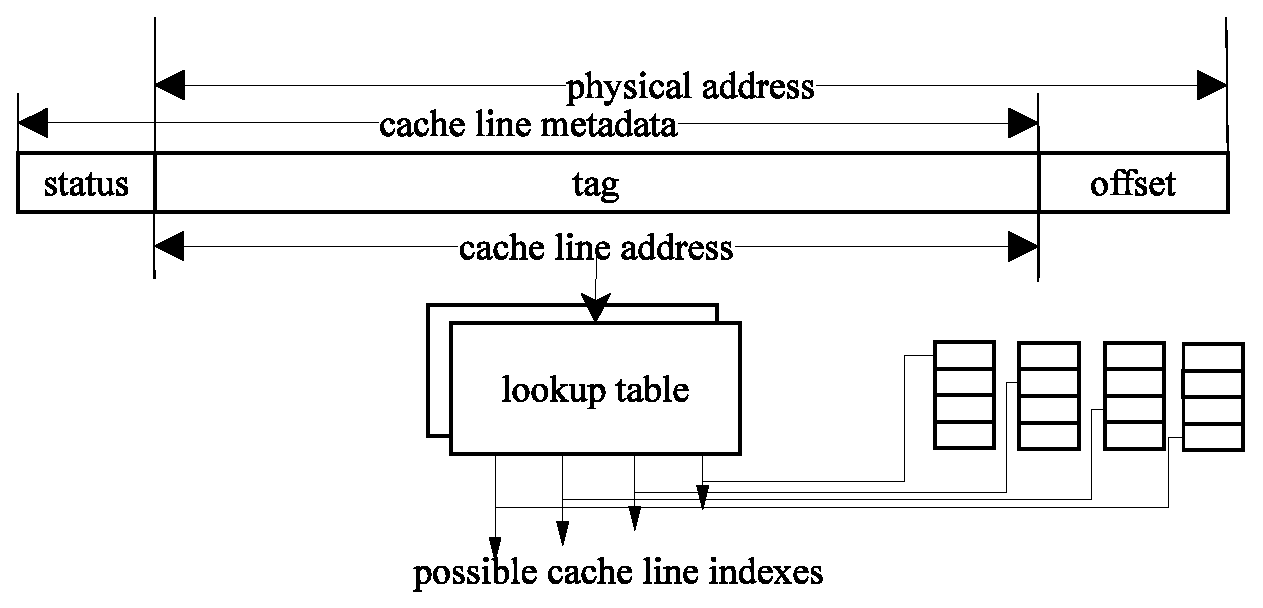
\includegraphics[width=\linewidth]{fig/dinome/scatter_tagarray.eps}
\resizebox{0.95\linewidth}{!}{\protect\footnotesize% Graphic for TeX using PGF
% Title: /Users/ziqiaozhou/zzdiss/paper/fig/scatter_tagarray_new.dia
% Creator: Dia v0.97.2
% CreationDate: Thu Jun 18 03:05:47 2020
% For: ziqiao
% \usepackage{tikz}
% The following commands are not supported in PSTricks at present
% We define them conditionally, so when they are implemented,
% this pgf file will use them.
\ifx\du\undefined
  \newlength{\du}
\fi
\setlength{\du}{15\unitlength}
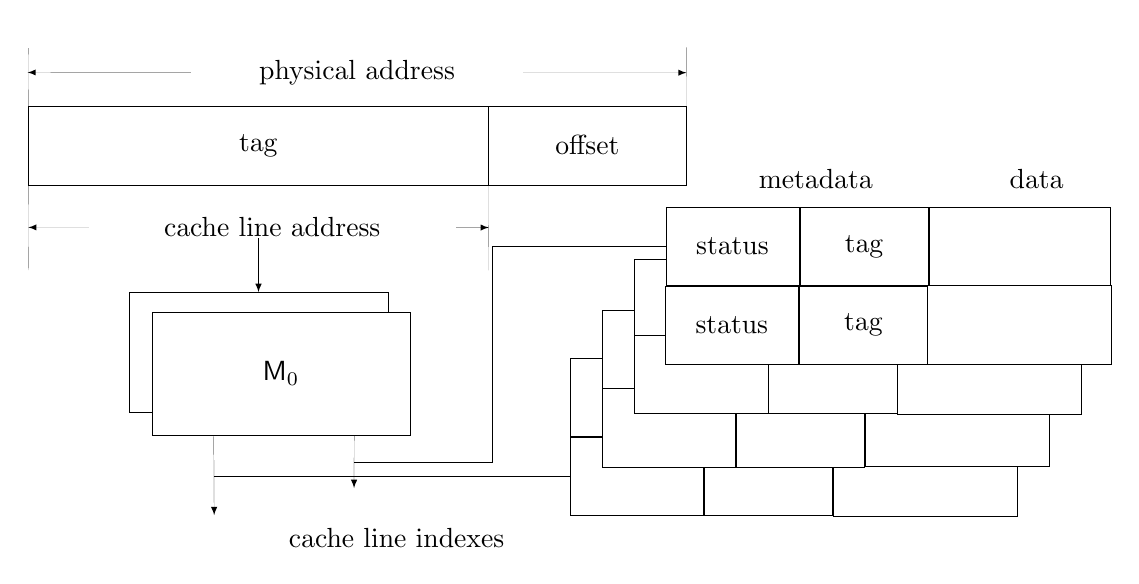
\begin{tikzpicture}
\pgftransformxscale{1.000000}
\pgftransformyscale{-1.000000}
\definecolor{dialinecolor}{rgb}{0.000000, 0.000000, 0.000000}
\pgfsetstrokecolor{dialinecolor}
\definecolor{dialinecolor}{rgb}{1.000000, 1.000000, 1.000000}
\pgfsetfillcolor{dialinecolor}
\pgfsetlinewidth{0.030000\du}
\pgfsetdash{}{0pt}
\pgfsetdash{}{0pt}
\pgfsetmiterjoin
\definecolor{dialinecolor}{rgb}{1.000000, 1.000000, 1.000000}
\pgfsetfillcolor{dialinecolor}
\fill (14.953400\du,7.517166\du)--(14.953400\du,8.517166\du)--(17.286231\du,8.517166\du)--(17.286231\du,7.517166\du)--cycle;
\definecolor{dialinecolor}{rgb}{0.000000, 0.000000, 0.000000}
\pgfsetstrokecolor{dialinecolor}
\draw (14.953400\du,7.517166\du)--(14.953400\du,8.517166\du)--(17.286231\du,8.517166\du)--(17.286231\du,7.517166\du)--cycle;
\pgfsetlinewidth{0.030000\du}
\pgfsetdash{}{0pt}
\pgfsetdash{}{0pt}
\pgfsetmiterjoin
\definecolor{dialinecolor}{rgb}{1.000000, 1.000000, 1.000000}
\pgfsetfillcolor{dialinecolor}
\fill (13.315500\du,7.518066\du)--(13.315500\du,8.510834\du)--(14.950876\du,8.510834\du)--(14.950876\du,7.518066\du)--cycle;
\definecolor{dialinecolor}{rgb}{0.000000, 0.000000, 0.000000}
\pgfsetstrokecolor{dialinecolor}
\draw (13.315500\du,7.518066\du)--(13.315500\du,8.510834\du)--(14.950876\du,8.510834\du)--(14.950876\du,7.518066\du)--cycle;
\pgfsetlinewidth{0.030000\du}
\pgfsetdash{}{0pt}
\pgfsetdash{}{0pt}
\pgfsetmiterjoin
\definecolor{dialinecolor}{rgb}{1.000000, 1.000000, 1.000000}
\pgfsetfillcolor{dialinecolor}
\fill (11.615900\du,7.518066\du)--(11.615900\du,8.510834\du)--(13.308313\du,8.510834\du)--(13.308313\du,7.518066\du)--cycle;
\definecolor{dialinecolor}{rgb}{0.000000, 0.000000, 0.000000}
\pgfsetstrokecolor{dialinecolor}
\draw (11.615900\du,7.518066\du)--(11.615900\du,8.510834\du)--(13.308313\du,8.510834\du)--(13.308313\du,7.518066\du)--cycle;
\pgfsetlinewidth{0.100000\du}
\pgfsetdash{{\pgflinewidth}{0.200000\du}}{0cm}
\pgfsetdash{{\pgflinewidth}{0.200000\du}}{0cm}
\pgfsetmiterjoin
\definecolor{dialinecolor}{rgb}{1.000000, 1.000000, 1.000000}
\pgfsetfillcolor{dialinecolor}
\fill (14.954200\du,8.520716\du)--(14.954200\du,9.520716\du)--(17.286265\du,9.520716\du)--(17.286265\du,8.520716\du)--cycle;
\definecolor{dialinecolor}{rgb}{0.000000, 0.000000, 0.000000}
\pgfsetstrokecolor{dialinecolor}
\draw (14.954200\du,8.520716\du)--(14.954200\du,9.520716\du)--(17.286265\du,9.520716\du)--(17.286265\du,8.520716\du)--cycle;
\pgfsetlinewidth{0.100000\du}
\pgfsetdash{{\pgflinewidth}{0.200000\du}}{0cm}
\pgfsetdash{{\pgflinewidth}{0.200000\du}}{0cm}
\pgfsetmiterjoin
\definecolor{dialinecolor}{rgb}{1.000000, 1.000000, 1.000000}
\pgfsetfillcolor{dialinecolor}
\fill (13.307300\du,8.513076\du)--(13.307300\du,9.505844\du)--(14.942676\du,9.505844\du)--(14.942676\du,8.513076\du)--cycle;
\definecolor{dialinecolor}{rgb}{0.000000, 0.000000, 0.000000}
\pgfsetstrokecolor{dialinecolor}
\draw (13.307300\du,8.513076\du)--(13.307300\du,9.505844\du)--(14.942676\du,9.505844\du)--(14.942676\du,8.513076\du)--cycle;
\pgfsetlinewidth{0.100000\du}
\pgfsetdash{{\pgflinewidth}{0.200000\du}}{0cm}
\pgfsetdash{{\pgflinewidth}{0.200000\du}}{0cm}
\pgfsetmiterjoin
\definecolor{dialinecolor}{rgb}{1.000000, 1.000000, 1.000000}
\pgfsetfillcolor{dialinecolor}
\fill (11.607700\du,8.513076\du)--(11.607700\du,9.505844\du)--(13.300113\du,9.505844\du)--(13.300113\du,8.513076\du)--cycle;
\definecolor{dialinecolor}{rgb}{0.000000, 0.000000, 0.000000}
\pgfsetstrokecolor{dialinecolor}
\draw (11.607700\du,8.513076\du)--(11.607700\du,9.505844\du)--(13.300113\du,9.505844\du)--(13.300113\du,8.513076\du)--cycle;
\pgfsetlinewidth{0.030000\du}
\pgfsetdash{}{0pt}
\pgfsetdash{}{0pt}
\pgfsetmiterjoin
\definecolor{dialinecolor}{rgb}{1.000000, 1.000000, 1.000000}
\pgfsetfillcolor{dialinecolor}
\fill (15.360200\du,6.904006\du)--(15.360200\du,7.904006\du)--(17.693031\du,7.904006\du)--(17.693031\du,6.904006\du)--cycle;
\definecolor{dialinecolor}{rgb}{0.000000, 0.000000, 0.000000}
\pgfsetstrokecolor{dialinecolor}
\draw (15.360200\du,6.904006\du)--(15.360200\du,7.904006\du)--(17.693031\du,7.904006\du)--(17.693031\du,6.904006\du)--cycle;
\pgfsetlinewidth{0.030000\du}
\pgfsetdash{}{0pt}
\pgfsetdash{}{0pt}
\pgfsetmiterjoin
\definecolor{dialinecolor}{rgb}{1.000000, 1.000000, 1.000000}
\pgfsetfillcolor{dialinecolor}
\fill (15.360900\du,7.890906\du)--(15.360900\du,8.890906\du)--(17.692965\du,8.890906\du)--(17.692965\du,7.890906\du)--cycle;
\definecolor{dialinecolor}{rgb}{0.000000, 0.000000, 0.000000}
\pgfsetstrokecolor{dialinecolor}
\draw (15.360900\du,7.890906\du)--(15.360900\du,8.890906\du)--(17.692965\du,8.890906\du)--(17.692965\du,7.890906\du)--cycle;
\pgfsetlinewidth{0.030000\du}
\pgfsetdash{}{0pt}
\pgfsetdash{}{0pt}
\pgfsetmiterjoin
\definecolor{dialinecolor}{rgb}{1.000000, 1.000000, 1.000000}
\pgfsetfillcolor{dialinecolor}
\fill (13.722200\du,6.904896\du)--(13.722200\du,7.897664\du)--(15.357576\du,7.897664\du)--(15.357576\du,6.904896\du)--cycle;
\definecolor{dialinecolor}{rgb}{0.000000, 0.000000, 0.000000}
\pgfsetstrokecolor{dialinecolor}
\draw (13.722200\du,6.904896\du)--(13.722200\du,7.897664\du)--(15.357576\du,7.897664\du)--(15.357576\du,6.904896\du)--cycle;
\pgfsetlinewidth{0.030000\du}
\pgfsetdash{}{0pt}
\pgfsetdash{}{0pt}
\pgfsetmiterjoin
\definecolor{dialinecolor}{rgb}{1.000000, 1.000000, 1.000000}
\pgfsetfillcolor{dialinecolor}
\fill (12.022700\du,6.904896\du)--(12.022700\du,7.897664\du)--(13.715113\du,7.897664\du)--(13.715113\du,6.904896\du)--cycle;
\definecolor{dialinecolor}{rgb}{0.000000, 0.000000, 0.000000}
\pgfsetstrokecolor{dialinecolor}
\draw (12.022700\du,6.904896\du)--(12.022700\du,7.897664\du)--(13.715113\du,7.897664\du)--(13.715113\du,6.904896\du)--cycle;
\pgfsetlinewidth{0.030000\du}
\pgfsetdash{}{0pt}
\pgfsetdash{}{0pt}
\pgfsetmiterjoin
\definecolor{dialinecolor}{rgb}{1.000000, 1.000000, 1.000000}
\pgfsetfillcolor{dialinecolor}
\fill (13.714000\du,7.899916\du)--(13.714000\du,8.892684\du)--(15.349376\du,8.892684\du)--(15.349376\du,7.899916\du)--cycle;
\definecolor{dialinecolor}{rgb}{0.000000, 0.000000, 0.000000}
\pgfsetstrokecolor{dialinecolor}
\draw (13.714000\du,7.899916\du)--(13.714000\du,8.892684\du)--(15.349376\du,8.892684\du)--(15.349376\du,7.899916\du)--cycle;
\pgfsetlinewidth{0.030000\du}
\pgfsetdash{}{0pt}
\pgfsetdash{}{0pt}
\pgfsetmiterjoin
\definecolor{dialinecolor}{rgb}{1.000000, 1.000000, 1.000000}
\pgfsetfillcolor{dialinecolor}
\fill (12.014500\du,7.899916\du)--(12.014500\du,8.892684\du)--(13.706913\du,8.892684\du)--(13.706913\du,7.899916\du)--cycle;
\definecolor{dialinecolor}{rgb}{0.000000, 0.000000, 0.000000}
\pgfsetstrokecolor{dialinecolor}
\draw (12.014500\du,7.899916\du)--(12.014500\du,8.892684\du)--(13.706913\du,8.892684\du)--(13.706913\du,7.899916\du)--cycle;
\pgfsetlinewidth{0.030000\du}
\pgfsetdash{}{0pt}
\pgfsetdash{}{0pt}
\pgfsetmiterjoin
\definecolor{dialinecolor}{rgb}{1.000000, 1.000000, 1.000000}
\pgfsetfillcolor{dialinecolor}
\fill (15.773700\du,6.261216\du)--(15.773700\du,7.261216\du)--(18.105765\du,7.261216\du)--(18.105765\du,6.261216\du)--cycle;
\definecolor{dialinecolor}{rgb}{0.000000, 0.000000, 0.000000}
\pgfsetstrokecolor{dialinecolor}
\draw (15.773700\du,6.261216\du)--(15.773700\du,7.261216\du)--(18.105765\du,7.261216\du)--(18.105765\du,6.261216\du)--cycle;
\pgfsetlinewidth{0.030000\du}
\pgfsetdash{}{0pt}
\pgfsetdash{}{0pt}
\pgfsetmiterjoin
\definecolor{dialinecolor}{rgb}{1.000000, 1.000000, 1.000000}
\pgfsetfillcolor{dialinecolor}
\fill (15.766600\du,7.223906\du)--(15.766600\du,8.223906\du)--(18.098665\du,8.223906\du)--(18.098665\du,7.223906\du)--cycle;
\definecolor{dialinecolor}{rgb}{0.000000, 0.000000, 0.000000}
\pgfsetstrokecolor{dialinecolor}
\draw (15.766600\du,7.223906\du)--(15.766600\du,8.223906\du)--(18.098665\du,8.223906\du)--(18.098665\du,7.223906\du)--cycle;
\pgfsetlinewidth{0.030000\du}
\pgfsetdash{}{0pt}
\pgfsetdash{}{0pt}
\pgfsetmiterjoin
\definecolor{dialinecolor}{rgb}{1.000000, 1.000000, 1.000000}
\pgfsetfillcolor{dialinecolor}
\fill (14.128000\du,6.255506\du)--(14.128000\du,7.248274\du)--(15.763376\du,7.248274\du)--(15.763376\du,6.255506\du)--cycle;
\definecolor{dialinecolor}{rgb}{0.000000, 0.000000, 0.000000}
\pgfsetstrokecolor{dialinecolor}
\draw (14.128000\du,6.255506\du)--(14.128000\du,7.248274\du)--(15.763376\du,7.248274\du)--(15.763376\du,6.255506\du)--cycle;
\pgfsetlinewidth{0.030000\du}
\pgfsetdash{}{0pt}
\pgfsetdash{}{0pt}
\pgfsetmiterjoin
\definecolor{dialinecolor}{rgb}{1.000000, 1.000000, 1.000000}
\pgfsetfillcolor{dialinecolor}
\fill (12.428400\du,6.255506\du)--(12.428400\du,7.248274\du)--(14.120813\du,7.248274\du)--(14.120813\du,6.255506\du)--cycle;
\definecolor{dialinecolor}{rgb}{0.000000, 0.000000, 0.000000}
\pgfsetstrokecolor{dialinecolor}
\draw (12.428400\du,6.255506\du)--(12.428400\du,7.248274\du)--(14.120813\du,7.248274\du)--(14.120813\du,6.255506\du)--cycle;
\pgfsetlinewidth{0.030000\du}
\pgfsetdash{}{0pt}
\pgfsetdash{}{0pt}
\pgfsetmiterjoin
\definecolor{dialinecolor}{rgb}{1.000000, 1.000000, 1.000000}
\pgfsetfillcolor{dialinecolor}
\fill (14.127100\du,7.226636\du)--(14.127100\du,8.219404\du)--(15.762476\du,8.219404\du)--(15.762476\du,7.226636\du)--cycle;
\definecolor{dialinecolor}{rgb}{0.000000, 0.000000, 0.000000}
\pgfsetstrokecolor{dialinecolor}
\draw (14.127100\du,7.226636\du)--(14.127100\du,8.219404\du)--(15.762476\du,8.219404\du)--(15.762476\du,7.226636\du)--cycle;
\pgfsetlinewidth{0.030000\du}
\pgfsetdash{}{0pt}
\pgfsetdash{}{0pt}
\pgfsetmiterjoin
\definecolor{dialinecolor}{rgb}{1.000000, 1.000000, 1.000000}
\pgfsetfillcolor{dialinecolor}
\fill (12.427500\du,7.226636\du)--(12.427500\du,8.219404\du)--(14.119913\du,8.219404\du)--(14.119913\du,7.226636\du)--cycle;
\definecolor{dialinecolor}{rgb}{0.000000, 0.000000, 0.000000}
\pgfsetstrokecolor{dialinecolor}
\draw (12.427500\du,7.226636\du)--(12.427500\du,8.219404\du)--(14.119913\du,8.219404\du)--(14.119913\du,7.226636\du)--cycle;
\definecolor{dialinecolor}{rgb}{1.000000, 1.000000, 1.000000}
\pgfsetfillcolor{dialinecolor}
\fill (13.576000\du,4.664585\du)--(13.576000\du,5.372085\du)--(15.886000\du,5.372085\du)--(15.886000\du,4.664585\du)--cycle;
% setfont left to latex
\definecolor{dialinecolor}{rgb}{0.000000, 0.000000, 0.000000}
\pgfsetstrokecolor{dialinecolor}
\node at (14.731000\du,5.234585\du){metadata};
\pgfsetlinewidth{0.080000\du}
\pgfsetdash{}{0pt}
\pgfsetdash{}{0pt}
\pgfsetmiterjoin
\pgfsetbuttcap
{
\definecolor{dialinecolor}{rgb}{0.000000, 0.000000, 0.000000}
\pgfsetfillcolor{dialinecolor}
% was here!!!
\pgfsetarrowsend{latex}
{\pgfsetcornersarced{\pgfpoint{0.000000\du}{0.000000\du}}\definecolor{dialinecolor}{rgb}{0.000000, 0.000000, 0.000000}
\pgfsetstrokecolor{dialinecolor}
\draw (7.651291\du,5.313240\du)--(7.651291\du,5.995305\du)--(7.654036\du,5.995305\du)--(7.654036\du,6.677370\du);
}}
\pgfsetlinewidth{0.080000\du}
\pgfsetdash{}{0pt}
\pgfsetdash{}{0pt}
\pgfsetmiterjoin
\pgfsetbuttcap
{
\definecolor{dialinecolor}{rgb}{0.000000, 0.000000, 0.000000}
\pgfsetfillcolor{dialinecolor}
% was here!!!
{\pgfsetcornersarced{\pgfpoint{0.000000\du}{0.000000\du}}\definecolor{dialinecolor}{rgb}{0.000000, 0.000000, 0.000000}
\pgfsetstrokecolor{dialinecolor}
\draw (8.868025\du,8.836026\du)--(10.625000\du,8.836026\du)--(10.625000\du,6.095930\du)--(12.827600\du,6.095930\du);
}}
% setfont left to latex
\definecolor{dialinecolor}{rgb}{0.000000, 0.000000, 0.000000}
\pgfsetstrokecolor{dialinecolor}
\node at (9.407599\du,9.793287\du){cache line indexes};
\pgfsetlinewidth{0.030000\du}
\pgfsetdash{}{0pt}
\pgfsetdash{}{0pt}
\pgfsetbuttcap
{
\definecolor{dialinecolor}{rgb}{0.000000, 0.000000, 0.000000}
\pgfsetfillcolor{dialinecolor}
% was here!!!
\pgfsetarrowsstart{latex}
\pgfsetarrowsend{latex}
\definecolor{dialinecolor}{rgb}{0.000000, 0.000000, 0.000000}
\pgfsetstrokecolor{dialinecolor}
\draw (4.731420\du,5.855600\du)--(10.577600\du,5.857115\du);
}
\definecolor{dialinecolor}{rgb}{1.000000, 1.000000, 1.000000}
\pgfsetfillcolor{dialinecolor}
\fill (5.496750\du,5.282290\du)--(5.496750\du,5.989790\du)--(10.159250\du,5.989790\du)--(10.159250\du,5.282290\du)--cycle;
% setfont left to latex
\definecolor{dialinecolor}{rgb}{0.000000, 0.000000, 0.000000}
\pgfsetstrokecolor{dialinecolor}
\node at (7.828000\du,5.852290\du){cache line address};
\pgfsetlinewidth{0.030000\du}
\pgfsetdash{}{0pt}
\pgfsetdash{}{0pt}
\pgfsetbuttcap
{
\definecolor{dialinecolor}{rgb}{0.000000, 0.000000, 0.000000}
\pgfsetfillcolor{dialinecolor}
% was here!!!
\definecolor{dialinecolor}{rgb}{0.000000, 0.000000, 0.000000}
\pgfsetstrokecolor{dialinecolor}
\draw (4.729300\du,5.313240\du)--(4.733540\du,6.397960\du);
}
\pgfsetlinewidth{0.030000\du}
\pgfsetdash{}{0pt}
\pgfsetdash{}{0pt}
\pgfsetbuttcap
{
\definecolor{dialinecolor}{rgb}{0.000000, 0.000000, 0.000000}
\pgfsetfillcolor{dialinecolor}
% was here!!!
\definecolor{dialinecolor}{rgb}{0.000000, 0.000000, 0.000000}
\pgfsetstrokecolor{dialinecolor}
\draw (10.575500\du,5.312920\du)--(10.579700\du,6.401310\du);
}
\pgfsetlinewidth{0.030000\du}
\pgfsetdash{}{0pt}
\pgfsetdash{}{0pt}
\pgfsetbuttcap
{
\definecolor{dialinecolor}{rgb}{0.000000, 0.000000, 0.000000}
\pgfsetfillcolor{dialinecolor}
% was here!!!
\definecolor{dialinecolor}{rgb}{0.000000, 0.000000, 0.000000}
\pgfsetstrokecolor{dialinecolor}
\draw (13.086300\du,3.570320\du)--(13.085100\du,4.312920\du);
}
\pgfsetlinewidth{0.030000\du}
\pgfsetdash{}{0pt}
\pgfsetdash{}{0pt}
\pgfsetbuttcap
{
\definecolor{dialinecolor}{rgb}{0.000000, 0.000000, 0.000000}
\pgfsetfillcolor{dialinecolor}
% was here!!!
\pgfsetarrowsstart{latex}
\pgfsetarrowsend{latex}
\definecolor{dialinecolor}{rgb}{0.000000, 0.000000, 0.000000}
\pgfsetstrokecolor{dialinecolor}
\draw (4.723030\du,3.887680\du)--(13.088300\du,3.890470\du);
}
\definecolor{dialinecolor}{rgb}{1.000000, 1.000000, 1.000000}
\pgfsetfillcolor{dialinecolor}
\fill (6.795665\du,3.319075\du)--(6.795665\du,4.026575\du)--(11.015665\du,4.026575\du)--(11.015665\du,3.319075\du)--cycle;
% setfont left to latex
\definecolor{dialinecolor}{rgb}{0.000000, 0.000000, 0.000000}
\pgfsetstrokecolor{dialinecolor}
\node at (8.905665\du,3.889075\du){physical address};
\pgfsetlinewidth{0.030000\du}
\pgfsetdash{}{0pt}
\pgfsetdash{}{0pt}
\pgfsetbuttcap
{
\definecolor{dialinecolor}{rgb}{0.000000, 0.000000, 0.000000}
\pgfsetfillcolor{dialinecolor}
% was here!!!
\definecolor{dialinecolor}{rgb}{0.000000, 0.000000, 0.000000}
\pgfsetstrokecolor{dialinecolor}
\draw (4.732750\du,3.578350\du)--(4.729300\du,4.313240\du);
}
\pgfsetlinewidth{0.050000\du}
\pgfsetdash{}{0pt}
\pgfsetdash{}{0pt}
\pgfsetmiterjoin
\definecolor{dialinecolor}{rgb}{1.000000, 1.000000, 1.000000}
\pgfsetfillcolor{dialinecolor}
\fill (4.729300\du,4.313240\du)--(4.729300\du,5.313240\du)--(10.573283\du,5.313240\du)--(10.573283\du,4.313240\du)--cycle;
\definecolor{dialinecolor}{rgb}{0.000000, 0.000000, 0.000000}
\pgfsetstrokecolor{dialinecolor}
\draw (4.729300\du,4.313240\du)--(4.729300\du,5.313240\du)--(10.573283\du,5.313240\du)--(10.573283\du,4.313240\du)--cycle;
% setfont left to latex
\definecolor{dialinecolor}{rgb}{0.000000, 0.000000, 0.000000}
\pgfsetstrokecolor{dialinecolor}
\node at (7.651290\du,4.813240\du){tag};
\pgfsetlinewidth{0.050000\du}
\pgfsetdash{}{0pt}
\pgfsetdash{}{0pt}
\pgfsetmiterjoin
\definecolor{dialinecolor}{rgb}{1.000000, 1.000000, 1.000000}
\pgfsetfillcolor{dialinecolor}
\fill (10.575500\du,4.312920\du)--(10.575500\du,5.312920\du)--(13.085145\du,5.312920\du)--(13.085145\du,4.312920\du)--cycle;
\definecolor{dialinecolor}{rgb}{0.000000, 0.000000, 0.000000}
\pgfsetstrokecolor{dialinecolor}
\draw (10.575500\du,4.312920\du)--(10.575500\du,5.312920\du)--(13.085145\du,5.312920\du)--(13.085145\du,4.312920\du)--cycle;
% setfont left to latex
\definecolor{dialinecolor}{rgb}{0.000000, 0.000000, 0.000000}
\pgfsetstrokecolor{dialinecolor}
\node at (11.830300\du,4.812920\du){offset};
\pgfsetlinewidth{0.030000\du}
\pgfsetdash{}{0pt}
\pgfsetdash{}{0pt}
\pgfsetmiterjoin
\definecolor{dialinecolor}{rgb}{1.000000, 1.000000, 1.000000}
\pgfsetfillcolor{dialinecolor}
\fill (14.518900\du,6.594556\du)--(14.518900\du,7.587324\du)--(16.154276\du,7.587324\du)--(16.154276\du,6.594556\du)--cycle;
\definecolor{dialinecolor}{rgb}{0.000000, 0.000000, 0.000000}
\pgfsetstrokecolor{dialinecolor}
\draw (14.518900\du,6.594556\du)--(14.518900\du,7.587324\du)--(16.154276\du,7.587324\du)--(16.154276\du,6.594556\du)--cycle;
\pgfsetlinewidth{0.030000\du}
\pgfsetdash{}{0pt}
\pgfsetdash{}{0pt}
\pgfsetmiterjoin
\definecolor{dialinecolor}{rgb}{1.000000, 1.000000, 1.000000}
\pgfsetfillcolor{dialinecolor}
\fill (12.819400\du,6.594556\du)--(12.819400\du,7.587324\du)--(14.511813\du,7.587324\du)--(14.511813\du,6.594556\du)--cycle;
\definecolor{dialinecolor}{rgb}{0.000000, 0.000000, 0.000000}
\pgfsetstrokecolor{dialinecolor}
\draw (12.819400\du,6.594556\du)--(12.819400\du,7.587324\du)--(14.511813\du,7.587324\du)--(14.511813\du,6.594556\du)--cycle;
% setfont left to latex
\definecolor{dialinecolor}{rgb}{0.000000, 0.000000, 0.000000}
\pgfsetstrokecolor{dialinecolor}
\node at (13.665606\du,7.090940\du){status};
% setfont left to latex
\definecolor{dialinecolor}{rgb}{0.000000, 0.000000, 0.000000}
\pgfsetstrokecolor{dialinecolor}
\node at (15.336588\du,7.090940\du){tag};
\pgfsetlinewidth{0.100000\du}
\pgfsetdash{{1.000000\du}{1.000000\du}}{0\du}
\pgfsetdash{{0.100000\du}{0.100000\du}}{0\du}
\pgfsetmiterjoin
\definecolor{dialinecolor}{rgb}{1.000000, 1.000000, 1.000000}
\pgfsetfillcolor{dialinecolor}
\fill (14.527100\du,5.599546\du)--(14.527100\du,6.592314\du)--(16.162476\du,6.592314\du)--(16.162476\du,5.599546\du)--cycle;
\definecolor{dialinecolor}{rgb}{0.000000, 0.000000, 0.000000}
\pgfsetstrokecolor{dialinecolor}
\draw (14.527100\du,5.599546\du)--(14.527100\du,6.592314\du)--(16.162476\du,6.592314\du)--(16.162476\du,5.599546\du)--cycle;
\pgfsetlinewidth{0.100000\du}
\pgfsetdash{{0.100000\du}{0.100000\du}}{0\du}
\pgfsetdash{{0.100000\du}{0.100000\du}}{0\du}
\pgfsetmiterjoin
\definecolor{dialinecolor}{rgb}{1.000000, 1.000000, 1.000000}
\pgfsetfillcolor{dialinecolor}
\fill (12.827600\du,5.599546\du)--(12.827600\du,6.592314\du)--(14.520013\du,6.592314\du)--(14.520013\du,5.599546\du)--cycle;
\definecolor{dialinecolor}{rgb}{0.000000, 0.000000, 0.000000}
\pgfsetstrokecolor{dialinecolor}
\draw (12.827600\du,5.599546\du)--(12.827600\du,6.592314\du)--(14.520013\du,6.592314\du)--(14.520013\du,5.599546\du)--cycle;
% setfont left to latex
\definecolor{dialinecolor}{rgb}{0.000000, 0.000000, 0.000000}
\pgfsetstrokecolor{dialinecolor}
\node at (13.673806\du,6.095930\du){status};
% setfont left to latex
\definecolor{dialinecolor}{rgb}{0.000000, 0.000000, 0.000000}
\pgfsetstrokecolor{dialinecolor}
\node at (15.344788\du,6.095930\du){tag};
\pgfsetlinewidth{0.030000\du}
\pgfsetdash{}{0pt}
\pgfsetdash{}{0pt}
\pgfsetmiterjoin
\definecolor{dialinecolor}{rgb}{1.000000, 1.000000, 1.000000}
\pgfsetfillcolor{dialinecolor}
\fill (16.143700\du,6.585556\du)--(16.143700\du,7.585556\du)--(18.475765\du,7.585556\du)--(18.475765\du,6.585556\du)--cycle;
\definecolor{dialinecolor}{rgb}{0.000000, 0.000000, 0.000000}
\pgfsetstrokecolor{dialinecolor}
\draw (16.143700\du,6.585556\du)--(16.143700\du,7.585556\du)--(18.475765\du,7.585556\du)--(18.475765\du,6.585556\du)--cycle;
\pgfsetlinewidth{0.100000\du}
\pgfsetdash{{1.000000\du}{1.000000\du}}{0\du}
\pgfsetdash{{0.100000\du}{0.100000\du}}{0\du}
\pgfsetmiterjoin
\definecolor{dialinecolor}{rgb}{1.000000, 1.000000, 1.000000}
\pgfsetfillcolor{dialinecolor}
\fill (16.165000\du,5.598646\du)--(16.165000\du,6.588899\du)--(18.466926\du,6.588899\du)--(18.466926\du,5.598646\du)--cycle;
\definecolor{dialinecolor}{rgb}{0.000000, 0.000000, 0.000000}
\pgfsetstrokecolor{dialinecolor}
\draw (16.165000\du,5.598646\du)--(16.165000\du,6.588899\du)--(18.466926\du,6.588899\du)--(18.466926\du,5.598646\du)--cycle;
\definecolor{dialinecolor}{rgb}{1.000000, 1.000000, 1.000000}
\pgfsetfillcolor{dialinecolor}
\fill (17.002250\du,4.667575\du)--(17.002250\du,5.375075\du)--(18.069750\du,5.375075\du)--(18.069750\du,4.667575\du)--cycle;
% setfont left to latex
\definecolor{dialinecolor}{rgb}{0.000000, 0.000000, 0.000000}
\pgfsetstrokecolor{dialinecolor}
\node at (17.536000\du,5.237575\du){data};
\pgfsetlinewidth{0.080000\du}
\pgfsetdash{}{0pt}
\pgfsetdash{}{0pt}
\pgfsetbuttcap
{
\definecolor{dialinecolor}{rgb}{0.000000, 0.000000, 0.000000}
\pgfsetfillcolor{dialinecolor}
% was here!!!
\pgfsetarrowsend{latex}
\definecolor{dialinecolor}{rgb}{0.000000, 0.000000, 0.000000}
\pgfsetstrokecolor{dialinecolor}
\draw (8.868570\du,8.505796\du)--(8.867480\du,9.166256\du);
}
\pgfsetlinewidth{0.080000\du}
\pgfsetdash{}{0pt}
\pgfsetdash{}{0pt}
\pgfsetbuttcap
{
\definecolor{dialinecolor}{rgb}{0.000000, 0.000000, 0.000000}
\pgfsetfillcolor{dialinecolor}
% was here!!!
\pgfsetarrowsend{latex}
\definecolor{dialinecolor}{rgb}{0.000000, 0.000000, 0.000000}
\pgfsetstrokecolor{dialinecolor}
\draw (7.085750\du,8.507996\du)--(7.090980\du,9.510936\du);
}
\pgfsetlinewidth{0.050000\du}
\pgfsetdash{}{0pt}
\pgfsetdash{}{0pt}
\pgfsetmiterjoin
\definecolor{dialinecolor}{rgb}{1.000000, 1.000000, 1.000000}
\pgfsetfillcolor{dialinecolor}
\fill (6.013821\du,6.677370\du)--(6.013821\du,8.205134\du)--(9.294250\du,8.205134\du)--(9.294250\du,6.677370\du)--cycle;
\definecolor{dialinecolor}{rgb}{0.000000, 0.000000, 0.000000}
\pgfsetstrokecolor{dialinecolor}
\draw (6.013821\du,6.677370\du)--(6.013821\du,8.205134\du)--(9.294250\du,8.205134\du)--(9.294250\du,6.677370\du)--cycle;
\pgfsetlinewidth{0.050000\du}
\pgfsetdash{}{0pt}
\pgfsetdash{}{0pt}
\pgfsetmiterjoin
\definecolor{dialinecolor}{rgb}{1.000000, 1.000000, 1.000000}
\pgfsetfillcolor{dialinecolor}
\fill (6.300070\du,6.924497\du)--(6.300070\du,8.493756\du)--(9.580499\du,8.493756\du)--(9.580499\du,6.924497\du)--cycle;
\definecolor{dialinecolor}{rgb}{0.000000, 0.000000, 0.000000}
\pgfsetstrokecolor{dialinecolor}
\draw (6.300070\du,6.924497\du)--(6.300070\du,8.493756\du)--(9.580499\du,8.493756\du)--(9.580499\du,6.924497\du)--cycle;
% setfont left to latex
\definecolor{dialinecolor}{rgb}{0.000000, 0.000000, 0.000000}
\pgfsetstrokecolor{dialinecolor}
\node at (7.940284\du,7.709126\du){\ensuremath{\cacheMap{0}}};
\pgfsetlinewidth{0.080000\du}
\pgfsetdash{}{0pt}
\pgfsetdash{}{0pt}
\pgfsetbuttcap
{
\definecolor{dialinecolor}{rgb}{0.000000, 0.000000, 0.000000}
\pgfsetfillcolor{dialinecolor}
% was here!!!
\definecolor{dialinecolor}{rgb}{0.000000, 0.000000, 0.000000}
\pgfsetstrokecolor{dialinecolor}
\draw (7.088365\du,9.009466\du)--(11.607700\du,9.009460\du);
}
\end{tikzpicture}
}
\caption{\scatterCache \label{fig:scatterTagarray}}
\endminipage
\centering
\minipage{0.49\textwidth}
%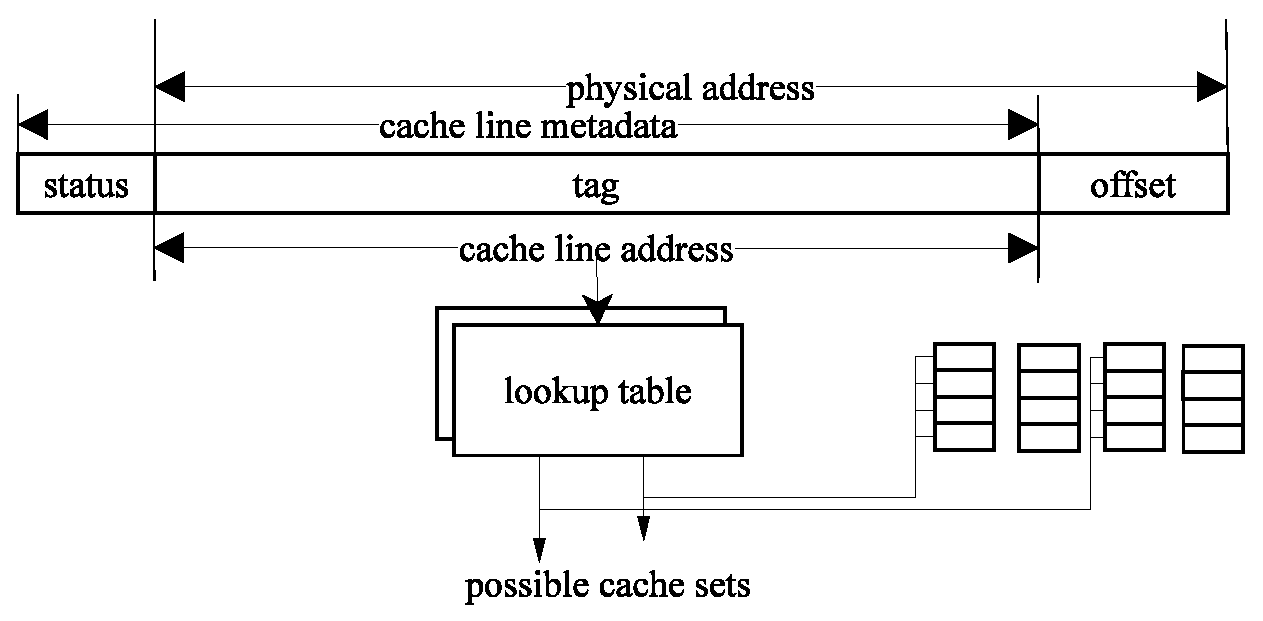
\includegraphics[width=\linewidth]{fig/dinome/phantom_tagarray.eps}
\resizebox{0.95\linewidth}{!}{\protect\footnotesize% Graphic for TeX using PGF
% Title: /Users/ziqiaozhou/zzdiss/paper/fig/phantom_tagarray_new.dia
% Creator: Dia v0.97.2
% CreationDate: Thu Jun 18 03:05:32 2020
% For: ziqiao
% \usepackage{tikz}
% The following commands are not supported in PSTricks at present
% We define them conditionally, so when they are implemented,
% this pgf file will use them.
\ifx\du\undefined
  \newlength{\du}
\fi
\setlength{\du}{15\unitlength}
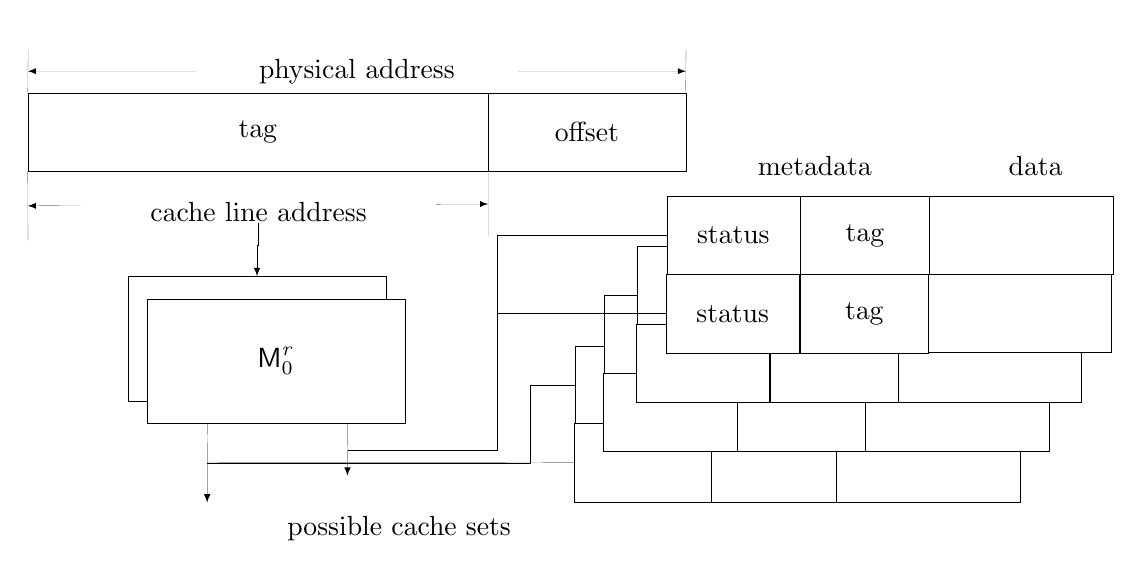
\begin{tikzpicture}
\pgftransformxscale{1.000000}
\pgftransformyscale{-1.000000}
\definecolor{dialinecolor}{rgb}{0.000000, 0.000000, 0.000000}
\pgfsetstrokecolor{dialinecolor}
\definecolor{dialinecolor}{rgb}{1.000000, 1.000000, 1.000000}
\pgfsetfillcolor{dialinecolor}
\pgfsetlinewidth{0.100000\du}
\pgfsetdash{{1.000000\du}{1.000000\du}}{0\du}
\pgfsetdash{{0.100000\du}{0.100000\du}}{0\du}
\pgfsetmiterjoin
\definecolor{dialinecolor}{rgb}{1.000000, 1.000000, 1.000000}
\pgfsetfillcolor{dialinecolor}
\fill (13.751400\du,8.540526\du)--(13.751400\du,9.533293\du)--(15.386776\du,9.533293\du)--(15.386776\du,8.540526\du)--cycle;
\definecolor{dialinecolor}{rgb}{0.000000, 0.000000, 0.000000}
\pgfsetstrokecolor{dialinecolor}
\draw (13.751400\du,8.540526\du)--(13.751400\du,9.533293\du)--(15.386776\du,9.533293\du)--(15.386776\du,8.540526\du)--cycle;
\pgfsetlinewidth{0.100000\du}
\pgfsetdash{{0.100000\du}{0.100000\du}}{0\du}
\pgfsetdash{{0.100000\du}{0.100000\du}}{0\du}
\pgfsetmiterjoin
\definecolor{dialinecolor}{rgb}{1.000000, 1.000000, 1.000000}
\pgfsetfillcolor{dialinecolor}
\fill (13.759600\du,7.545516\du)--(13.759600\du,8.538283\du)--(15.394976\du,8.538283\du)--(15.394976\du,7.545516\du)--cycle;
\definecolor{dialinecolor}{rgb}{0.000000, 0.000000, 0.000000}
\pgfsetstrokecolor{dialinecolor}
\draw (13.759600\du,7.545516\du)--(13.759600\du,8.538283\du)--(15.394976\du,8.538283\du)--(15.394976\du,7.545516\du)--cycle;
\pgfsetlinewidth{0.100000\du}
\pgfsetdash{{0.100000\du}{0.100000\du}}{0\du}
\pgfsetdash{{0.100000\du}{0.100000\du}}{0\du}
\pgfsetmiterjoin
\definecolor{dialinecolor}{rgb}{1.000000, 1.000000, 1.000000}
\pgfsetfillcolor{dialinecolor}
\fill (12.060100\du,7.545516\du)--(12.060100\du,8.538283\du)--(13.803126\du,8.538283\du)--(13.803126\du,7.545516\du)--cycle;
\definecolor{dialinecolor}{rgb}{0.000000, 0.000000, 0.000000}
\pgfsetstrokecolor{dialinecolor}
\draw (12.060100\du,7.545516\du)--(12.060100\du,8.538283\du)--(13.803126\du,8.538283\du)--(13.803126\du,7.545516\du)--cycle;
\pgfsetlinewidth{0.100000\du}
\pgfsetdash{{0.100000\du}{0.100000\du}}{0\du}
\pgfsetdash{{0.100000\du}{0.100000\du}}{0\du}
\pgfsetmiterjoin
\definecolor{dialinecolor}{rgb}{1.000000, 1.000000, 1.000000}
\pgfsetfillcolor{dialinecolor}
\fill (15.376200\du,8.531526\du)--(15.376200\du,9.531526\du)--(17.708265\du,9.531526\du)--(17.708265\du,8.531526\du)--cycle;
\definecolor{dialinecolor}{rgb}{0.000000, 0.000000, 0.000000}
\pgfsetstrokecolor{dialinecolor}
\draw (15.376200\du,8.531526\du)--(15.376200\du,9.531526\du)--(17.708265\du,9.531526\du)--(17.708265\du,8.531526\du)--cycle;
\pgfsetlinewidth{0.100000\du}
\pgfsetdash{{0.100000\du}{0.100000\du}}{0\du}
\pgfsetdash{{0.100000\du}{0.100000\du}}{0\du}
\pgfsetmiterjoin
\definecolor{dialinecolor}{rgb}{1.000000, 1.000000, 1.000000}
\pgfsetfillcolor{dialinecolor}
\fill (15.397600\du,7.544616\du)--(15.397600\du,8.534869\du)--(17.730431\du,8.534869\du)--(17.730431\du,7.544616\du)--cycle;
\definecolor{dialinecolor}{rgb}{0.000000, 0.000000, 0.000000}
\pgfsetstrokecolor{dialinecolor}
\draw (15.397600\du,7.544616\du)--(15.397600\du,8.534869\du)--(17.730431\du,8.534869\du)--(17.730431\du,7.544616\du)--cycle;
\pgfsetlinewidth{0.100000\du}
\pgfsetdash{{0.100000\du}{0.100000\du}}{0\du}
\pgfsetdash{{0.100000\du}{0.100000\du}}{0\du}
\pgfsetmiterjoin
\definecolor{dialinecolor}{rgb}{1.000000, 1.000000, 1.000000}
\pgfsetfillcolor{dialinecolor}
\fill (12.048300\du,8.528306\du)--(12.048300\du,9.521073\du)--(13.791326\du,9.521073\du)--(13.791326\du,8.528306\du)--cycle;
\definecolor{dialinecolor}{rgb}{0.000000, 0.000000, 0.000000}
\pgfsetstrokecolor{dialinecolor}
\draw (12.048300\du,8.528306\du)--(12.048300\du,9.521073\du)--(13.791326\du,9.521073\du)--(13.791326\du,8.528306\du)--cycle;
\pgfsetlinewidth{0.030000\du}
\pgfsetdash{}{0pt}
\pgfsetdash{}{0pt}
\pgfsetmiterjoin
\definecolor{dialinecolor}{rgb}{1.000000, 1.000000, 1.000000}
\pgfsetfillcolor{dialinecolor}
\fill (14.118400\du,7.888695\du)--(14.118400\du,8.881463\du)--(15.753776\du,8.881463\du)--(15.753776\du,7.888695\du)--cycle;
\definecolor{dialinecolor}{rgb}{0.000000, 0.000000, 0.000000}
\pgfsetstrokecolor{dialinecolor}
\draw (14.118400\du,7.888695\du)--(14.118400\du,8.881463\du)--(15.753776\du,8.881463\du)--(15.753776\du,7.888695\du)--cycle;
\pgfsetlinewidth{0.030000\du}
\pgfsetdash{}{0pt}
\pgfsetdash{}{0pt}
\pgfsetmiterjoin
\definecolor{dialinecolor}{rgb}{1.000000, 1.000000, 1.000000}
\pgfsetfillcolor{dialinecolor}
\fill (12.418800\du,7.888695\du)--(12.418800\du,8.881463\du)--(14.111213\du,8.881463\du)--(14.111213\du,7.888695\du)--cycle;
\definecolor{dialinecolor}{rgb}{0.000000, 0.000000, 0.000000}
\pgfsetstrokecolor{dialinecolor}
\draw (12.418800\du,7.888695\du)--(12.418800\du,8.881463\du)--(14.111213\du,8.881463\du)--(14.111213\du,7.888695\du)--cycle;
\pgfsetlinewidth{0.030000\du}
\pgfsetdash{}{0pt}
\pgfsetdash{}{0pt}
\pgfsetmiterjoin
\definecolor{dialinecolor}{rgb}{1.000000, 1.000000, 1.000000}
\pgfsetfillcolor{dialinecolor}
\fill (14.126600\du,6.893685\du)--(14.126600\du,7.886453\du)--(15.761976\du,7.886453\du)--(15.761976\du,6.893685\du)--cycle;
\definecolor{dialinecolor}{rgb}{0.000000, 0.000000, 0.000000}
\pgfsetstrokecolor{dialinecolor}
\draw (14.126600\du,6.893685\du)--(14.126600\du,7.886453\du)--(15.761976\du,7.886453\du)--(15.761976\du,6.893685\du)--cycle;
\pgfsetlinewidth{0.030000\du}
\pgfsetdash{}{0pt}
\pgfsetdash{}{0pt}
\pgfsetmiterjoin
\definecolor{dialinecolor}{rgb}{1.000000, 1.000000, 1.000000}
\pgfsetfillcolor{dialinecolor}
\fill (12.427000\du,6.893685\du)--(12.427000\du,7.886453\du)--(14.119413\du,7.886453\du)--(14.119413\du,6.893685\du)--cycle;
\definecolor{dialinecolor}{rgb}{0.000000, 0.000000, 0.000000}
\pgfsetstrokecolor{dialinecolor}
\draw (12.427000\du,6.893685\du)--(12.427000\du,7.886453\du)--(14.119413\du,7.886453\du)--(14.119413\du,6.893685\du)--cycle;
\pgfsetlinewidth{0.030000\du}
\pgfsetdash{}{0pt}
\pgfsetdash{}{0pt}
\pgfsetmiterjoin
\definecolor{dialinecolor}{rgb}{1.000000, 1.000000, 1.000000}
\pgfsetfillcolor{dialinecolor}
\fill (15.743100\du,7.879695\du)--(15.743100\du,8.879695\du)--(18.075165\du,8.879695\du)--(18.075165\du,7.879695\du)--cycle;
\definecolor{dialinecolor}{rgb}{0.000000, 0.000000, 0.000000}
\pgfsetstrokecolor{dialinecolor}
\draw (15.743100\du,7.879695\du)--(15.743100\du,8.879695\du)--(18.075165\du,8.879695\du)--(18.075165\du,7.879695\du)--cycle;
\pgfsetlinewidth{0.030000\du}
\pgfsetdash{}{0pt}
\pgfsetdash{}{0pt}
\pgfsetmiterjoin
\definecolor{dialinecolor}{rgb}{1.000000, 1.000000, 1.000000}
\pgfsetfillcolor{dialinecolor}
\fill (15.764500\du,6.892785\du)--(15.764500\du,7.883038\du)--(18.097331\du,7.883038\du)--(18.097331\du,6.892785\du)--cycle;
\definecolor{dialinecolor}{rgb}{0.000000, 0.000000, 0.000000}
\pgfsetstrokecolor{dialinecolor}
\draw (15.764500\du,6.892785\du)--(15.764500\du,7.883038\du)--(18.097331\du,7.883038\du)--(18.097331\du,6.892785\du)--cycle;
\pgfsetlinewidth{0.050000\du}
\pgfsetdash{}{0pt}
\pgfsetdash{}{0pt}
\pgfsetmiterjoin
\definecolor{dialinecolor}{rgb}{1.000000, 1.000000, 1.000000}
\pgfsetfillcolor{dialinecolor}
\fill (6.379780\du,6.658681\du)--(6.379780\du,8.243927\du)--(9.660209\du,8.243927\du)--(9.660209\du,6.658681\du)--cycle;
\definecolor{dialinecolor}{rgb}{0.000000, 0.000000, 0.000000}
\pgfsetstrokecolor{dialinecolor}
\draw (6.379780\du,6.658681\du)--(6.379780\du,8.243927\du)--(9.660209\du,8.243927\du)--(9.660209\du,6.658681\du)--cycle;
\pgfsetlinewidth{0.080000\du}
\pgfsetdash{}{0pt}
\pgfsetdash{}{0pt}
\pgfsetmiterjoin
\pgfsetbuttcap
{
\definecolor{dialinecolor}{rgb}{0.000000, 0.000000, 0.000000}
\pgfsetfillcolor{dialinecolor}
% was here!!!
\pgfsetarrowsend{latex}
{\pgfsetcornersarced{\pgfpoint{0.000000\du}{0.000000\du}}\definecolor{dialinecolor}{rgb}{0.000000, 0.000000, 0.000000}
\pgfsetstrokecolor{dialinecolor}
\draw (8.030260\du,5.325730\du)--(8.030260\du,6.260100\du)--(8.019994\du,6.260100\du)--(8.019994\du,6.658681\du);
}}
\pgfsetlinewidth{0.080000\du}
\pgfsetdash{}{0pt}
\pgfsetdash{}{0pt}
\pgfsetbuttcap
{
\definecolor{dialinecolor}{rgb}{0.000000, 0.000000, 0.000000}
\pgfsetfillcolor{dialinecolor}
% was here!!!
\pgfsetarrowsend{latex}
\definecolor{dialinecolor}{rgb}{0.000000, 0.000000, 0.000000}
\pgfsetstrokecolor{dialinecolor}
\draw (9.172990\du,8.527596\du)--(9.167870\du,9.192426\du);
}
\pgfsetlinewidth{0.080000\du}
\pgfsetdash{}{0pt}
\pgfsetdash{}{0pt}
\pgfsetbuttcap
{
\definecolor{dialinecolor}{rgb}{0.000000, 0.000000, 0.000000}
\pgfsetfillcolor{dialinecolor}
% was here!!!
\pgfsetarrowsend{latex}
\definecolor{dialinecolor}{rgb}{0.000000, 0.000000, 0.000000}
\pgfsetstrokecolor{dialinecolor}
\draw (7.390160\du,8.523196\du)--(7.386740\du,9.533366\du);
}
% setfont left to latex
\definecolor{dialinecolor}{rgb}{0.000000, 0.000000, 0.000000}
\pgfsetstrokecolor{dialinecolor}
\node at (9.824187\du,9.868416\du){possible cache sets};
\pgfsetlinewidth{0.030000\du}
\pgfsetdash{}{0pt}
\pgfsetdash{}{0pt}
\pgfsetbuttcap
{
\definecolor{dialinecolor}{rgb}{0.000000, 0.000000, 0.000000}
\pgfsetfillcolor{dialinecolor}
% was here!!!
\pgfsetarrowsstart{latex}
\pgfsetarrowsend{latex}
\definecolor{dialinecolor}{rgb}{0.000000, 0.000000, 0.000000}
\pgfsetstrokecolor{dialinecolor}
\draw (5.110015\du,5.763980\du)--(10.954550\du,5.740960\du);
}
\definecolor{dialinecolor}{rgb}{1.000000, 1.000000, 1.000000}
\pgfsetfillcolor{dialinecolor}
\fill (5.783770\du,5.290130\du)--(5.783770\du,5.977630\du)--(10.296270\du,5.977630\du)--(10.296270\du,5.290130\du)--cycle;
% setfont left to latex
\definecolor{dialinecolor}{rgb}{0.000000, 0.000000, 0.000000}
\pgfsetstrokecolor{dialinecolor}
\node at (8.040020\du,5.842630\du){cache line address};
\pgfsetlinewidth{0.030000\du}
\pgfsetdash{}{0pt}
\pgfsetdash{}{0pt}
\pgfsetbuttcap
{
\definecolor{dialinecolor}{rgb}{0.000000, 0.000000, 0.000000}
\pgfsetfillcolor{dialinecolor}
% was here!!!
\definecolor{dialinecolor}{rgb}{0.000000, 0.000000, 0.000000}
\pgfsetstrokecolor{dialinecolor}
\draw (5.108270\du,5.325730\du)--(5.111760\du,6.202230\du);
}
\pgfsetlinewidth{0.030000\du}
\pgfsetdash{}{0pt}
\pgfsetdash{}{0pt}
\pgfsetbuttcap
{
\definecolor{dialinecolor}{rgb}{0.000000, 0.000000, 0.000000}
\pgfsetfillcolor{dialinecolor}
% was here!!!
\definecolor{dialinecolor}{rgb}{0.000000, 0.000000, 0.000000}
\pgfsetstrokecolor{dialinecolor}
\draw (10.954400\du,5.326320\du)--(10.954700\du,6.155600\du);
}
\pgfsetlinewidth{0.030000\du}
\pgfsetdash{}{0pt}
\pgfsetdash{}{0pt}
\pgfsetbuttcap
{
\definecolor{dialinecolor}{rgb}{0.000000, 0.000000, 0.000000}
\pgfsetfillcolor{dialinecolor}
% was here!!!
\pgfsetarrowsstart{latex}
\pgfsetarrowsend{latex}
\definecolor{dialinecolor}{rgb}{0.000000, 0.000000, 0.000000}
\pgfsetstrokecolor{dialinecolor}
\draw (5.110770\du,4.053755\du)--(13.466300\du,4.054050\du);
}
\definecolor{dialinecolor}{rgb}{1.000000, 1.000000, 1.000000}
\pgfsetfillcolor{dialinecolor}
\fill (7.243535\du,3.501405\du)--(7.243535\du,4.188905\du)--(11.333535\du,4.188905\du)--(11.333535\du,3.501405\du)--cycle;
% setfont left to latex
\definecolor{dialinecolor}{rgb}{0.000000, 0.000000, 0.000000}
\pgfsetstrokecolor{dialinecolor}
\node at (9.288535\du,4.053905\du){physical address};
\pgfsetlinewidth{0.030000\du}
\pgfsetdash{}{0pt}
\pgfsetdash{}{0pt}
\pgfsetbuttcap
{
\definecolor{dialinecolor}{rgb}{0.000000, 0.000000, 0.000000}
\pgfsetfillcolor{dialinecolor}
% was here!!!
\definecolor{dialinecolor}{rgb}{0.000000, 0.000000, 0.000000}
\pgfsetstrokecolor{dialinecolor}
\draw (5.113270\du,3.781780\du)--(5.108270\du,4.325730\du);
}
\pgfsetlinewidth{0.030000\du}
\pgfsetdash{}{0pt}
\pgfsetdash{}{0pt}
\pgfsetbuttcap
{
\definecolor{dialinecolor}{rgb}{0.000000, 0.000000, 0.000000}
\pgfsetfillcolor{dialinecolor}
% was here!!!
\definecolor{dialinecolor}{rgb}{0.000000, 0.000000, 0.000000}
\pgfsetstrokecolor{dialinecolor}
\draw (13.468600\du,3.781780\du)--(13.464000\du,4.326320\du);
}
\pgfsetlinewidth{0.050000\du}
\pgfsetdash{}{0pt}
\pgfsetdash{}{0pt}
\pgfsetmiterjoin
\definecolor{dialinecolor}{rgb}{1.000000, 1.000000, 1.000000}
\pgfsetfillcolor{dialinecolor}
\fill (5.108270\du,4.325730\du)--(5.108270\du,5.325730\du)--(10.952253\du,5.325730\du)--(10.952253\du,4.325730\du)--cycle;
\definecolor{dialinecolor}{rgb}{0.000000, 0.000000, 0.000000}
\pgfsetstrokecolor{dialinecolor}
\draw (5.108270\du,4.325730\du)--(5.108270\du,5.325730\du)--(10.952253\du,5.325730\du)--(10.952253\du,4.325730\du)--cycle;
% setfont left to latex
\definecolor{dialinecolor}{rgb}{0.000000, 0.000000, 0.000000}
\pgfsetstrokecolor{dialinecolor}
\node at (8.030260\du,4.825730\du){tag};
\pgfsetlinewidth{0.050000\du}
\pgfsetdash{}{0pt}
\pgfsetdash{}{0pt}
\pgfsetmiterjoin
\definecolor{dialinecolor}{rgb}{1.000000, 1.000000, 1.000000}
\pgfsetfillcolor{dialinecolor}
\fill (10.954400\du,4.326320\du)--(10.954400\du,5.326320\du)--(13.464045\du,5.326320\du)--(13.464045\du,4.326320\du)--cycle;
\definecolor{dialinecolor}{rgb}{0.000000, 0.000000, 0.000000}
\pgfsetstrokecolor{dialinecolor}
\draw (10.954400\du,4.326320\du)--(10.954400\du,5.326320\du)--(13.464045\du,5.326320\du)--(13.464045\du,4.326320\du)--cycle;
% setfont left to latex
\definecolor{dialinecolor}{rgb}{0.000000, 0.000000, 0.000000}
\pgfsetstrokecolor{dialinecolor}
\node at (12.209200\du,4.826320\du){offset};
\pgfsetlinewidth{0.030000\du}
\pgfsetdash{}{0pt}
\pgfsetdash{}{0pt}
\pgfsetmiterjoin
\definecolor{dialinecolor}{rgb}{1.000000, 1.000000, 1.000000}
\pgfsetfillcolor{dialinecolor}
\fill (14.532300\du,7.267677\du)--(14.532300\du,8.260445\du)--(16.167676\du,8.260445\du)--(16.167676\du,7.267677\du)--cycle;
\definecolor{dialinecolor}{rgb}{0.000000, 0.000000, 0.000000}
\pgfsetstrokecolor{dialinecolor}
\draw (14.532300\du,7.267677\du)--(14.532300\du,8.260445\du)--(16.167676\du,8.260445\du)--(16.167676\du,7.267677\du)--cycle;
\pgfsetlinewidth{0.030000\du}
\pgfsetdash{}{0pt}
\pgfsetdash{}{0pt}
\pgfsetmiterjoin
\definecolor{dialinecolor}{rgb}{1.000000, 1.000000, 1.000000}
\pgfsetfillcolor{dialinecolor}
\fill (12.832700\du,7.267677\du)--(12.832700\du,8.260445\du)--(14.525113\du,8.260445\du)--(14.525113\du,7.267677\du)--cycle;
\definecolor{dialinecolor}{rgb}{0.000000, 0.000000, 0.000000}
\pgfsetstrokecolor{dialinecolor}
\draw (12.832700\du,7.267677\du)--(12.832700\du,8.260445\du)--(14.525113\du,8.260445\du)--(14.525113\du,7.267677\du)--cycle;
\pgfsetlinewidth{0.030000\du}
\pgfsetdash{}{0pt}
\pgfsetdash{}{0pt}
\pgfsetmiterjoin
\definecolor{dialinecolor}{rgb}{1.000000, 1.000000, 1.000000}
\pgfsetfillcolor{dialinecolor}
\fill (14.540500\du,6.272667\du)--(14.540500\du,7.265435\du)--(16.175876\du,7.265435\du)--(16.175876\du,6.272667\du)--cycle;
\definecolor{dialinecolor}{rgb}{0.000000, 0.000000, 0.000000}
\pgfsetstrokecolor{dialinecolor}
\draw (14.540500\du,6.272667\du)--(14.540500\du,7.265435\du)--(16.175876\du,7.265435\du)--(16.175876\du,6.272667\du)--cycle;
\pgfsetlinewidth{0.030000\du}
\pgfsetdash{}{0pt}
\pgfsetdash{}{0pt}
\pgfsetmiterjoin
\definecolor{dialinecolor}{rgb}{1.000000, 1.000000, 1.000000}
\pgfsetfillcolor{dialinecolor}
\fill (12.840900\du,6.272667\du)--(12.840900\du,7.265435\du)--(14.533313\du,7.265435\du)--(14.533313\du,6.272667\du)--cycle;
\definecolor{dialinecolor}{rgb}{0.000000, 0.000000, 0.000000}
\pgfsetstrokecolor{dialinecolor}
\draw (12.840900\du,6.272667\du)--(12.840900\du,7.265435\du)--(14.533313\du,7.265435\du)--(14.533313\du,6.272667\du)--cycle;
\pgfsetlinewidth{0.030000\du}
\pgfsetdash{}{0pt}
\pgfsetdash{}{0pt}
\pgfsetmiterjoin
\definecolor{dialinecolor}{rgb}{1.000000, 1.000000, 1.000000}
\pgfsetfillcolor{dialinecolor}
\fill (16.157000\du,7.258677\du)--(16.157000\du,8.258677\du)--(18.489065\du,8.258677\du)--(18.489065\du,7.258677\du)--cycle;
\definecolor{dialinecolor}{rgb}{0.000000, 0.000000, 0.000000}
\pgfsetstrokecolor{dialinecolor}
\draw (16.157000\du,7.258677\du)--(16.157000\du,8.258677\du)--(18.489065\du,8.258677\du)--(18.489065\du,7.258677\du)--cycle;
\pgfsetlinewidth{0.030000\du}
\pgfsetdash{}{0pt}
\pgfsetdash{}{0pt}
\pgfsetmiterjoin
\definecolor{dialinecolor}{rgb}{1.000000, 1.000000, 1.000000}
\pgfsetfillcolor{dialinecolor}
\fill (16.178400\du,6.271767\du)--(16.178400\du,7.262021\du)--(18.511231\du,7.262021\du)--(18.511231\du,6.271767\du)--cycle;
\definecolor{dialinecolor}{rgb}{0.000000, 0.000000, 0.000000}
\pgfsetstrokecolor{dialinecolor}
\draw (16.178400\du,6.271767\du)--(16.178400\du,7.262021\du)--(18.511231\du,7.262021\du)--(18.511231\du,6.271767\du)--cycle;
\pgfsetlinewidth{0.100000\du}
\pgfsetdash{{1.000000\du}{1.000000\du}}{0\du}
\pgfsetdash{{0.100000\du}{0.100000\du}}{0\du}
\pgfsetmiterjoin
\definecolor{dialinecolor}{rgb}{1.000000, 1.000000, 1.000000}
\pgfsetfillcolor{dialinecolor}
\fill (14.914500\du,6.635819\du)--(14.914500\du,7.628587\du)--(16.549876\du,7.628587\du)--(16.549876\du,6.635819\du)--cycle;
\definecolor{dialinecolor}{rgb}{0.000000, 0.000000, 0.000000}
\pgfsetstrokecolor{dialinecolor}
\draw (14.914500\du,6.635819\du)--(14.914500\du,7.628587\du)--(16.549876\du,7.628587\du)--(16.549876\du,6.635819\du)--cycle;
\pgfsetlinewidth{0.100000\du}
\pgfsetdash{{0.100000\du}{0.100000\du}}{0\du}
\pgfsetdash{{0.100000\du}{0.100000\du}}{0\du}
\pgfsetmiterjoin
\definecolor{dialinecolor}{rgb}{1.000000, 1.000000, 1.000000}
\pgfsetfillcolor{dialinecolor}
\fill (13.214900\du,6.635819\du)--(13.214900\du,7.628587\du)--(14.907313\du,7.628587\du)--(14.907313\du,6.635819\du)--cycle;
\definecolor{dialinecolor}{rgb}{0.000000, 0.000000, 0.000000}
\pgfsetstrokecolor{dialinecolor}
\draw (13.214900\du,6.635819\du)--(13.214900\du,7.628587\du)--(14.907313\du,7.628587\du)--(14.907313\du,6.635819\du)--cycle;
% setfont left to latex
\definecolor{dialinecolor}{rgb}{0.000000, 0.000000, 0.000000}
\pgfsetstrokecolor{dialinecolor}
\node at (14.061106\du,7.132203\du){status};
% setfont left to latex
\definecolor{dialinecolor}{rgb}{0.000000, 0.000000, 0.000000}
\pgfsetstrokecolor{dialinecolor}
\node at (15.732188\du,7.132203\du){tag};
\pgfsetlinewidth{0.100000\du}
\pgfsetdash{{0.100000\du}{0.100000\du}}{0\du}
\pgfsetdash{{0.100000\du}{0.100000\du}}{0\du}
\pgfsetmiterjoin
\definecolor{dialinecolor}{rgb}{1.000000, 1.000000, 1.000000}
\pgfsetfillcolor{dialinecolor}
\fill (14.922700\du,5.640809\du)--(14.922700\du,6.633577\du)--(16.558076\du,6.633577\du)--(16.558076\du,5.640809\du)--cycle;
\definecolor{dialinecolor}{rgb}{0.000000, 0.000000, 0.000000}
\pgfsetstrokecolor{dialinecolor}
\draw (14.922700\du,5.640809\du)--(14.922700\du,6.633577\du)--(16.558076\du,6.633577\du)--(16.558076\du,5.640809\du)--cycle;
\pgfsetlinewidth{0.100000\du}
\pgfsetdash{{0.100000\du}{0.100000\du}}{0\du}
\pgfsetdash{{0.100000\du}{0.100000\du}}{0\du}
\pgfsetmiterjoin
\definecolor{dialinecolor}{rgb}{1.000000, 1.000000, 1.000000}
\pgfsetfillcolor{dialinecolor}
\fill (13.223100\du,5.640809\du)--(13.223100\du,6.633577\du)--(14.915513\du,6.633577\du)--(14.915513\du,5.640809\du)--cycle;
\definecolor{dialinecolor}{rgb}{0.000000, 0.000000, 0.000000}
\pgfsetstrokecolor{dialinecolor}
\draw (13.223100\du,5.640809\du)--(13.223100\du,6.633577\du)--(14.915513\du,6.633577\du)--(14.915513\du,5.640809\du)--cycle;
% setfont left to latex
\definecolor{dialinecolor}{rgb}{0.000000, 0.000000, 0.000000}
\pgfsetstrokecolor{dialinecolor}
\node at (14.069306\du,6.137193\du){status};
% setfont left to latex
\definecolor{dialinecolor}{rgb}{0.000000, 0.000000, 0.000000}
\pgfsetstrokecolor{dialinecolor}
\node at (15.740388\du,6.137193\du){tag};
\pgfsetlinewidth{0.100000\du}
\pgfsetdash{{0.100000\du}{0.100000\du}}{0\du}
\pgfsetdash{{0.100000\du}{0.100000\du}}{0\du}
\pgfsetmiterjoin
\definecolor{dialinecolor}{rgb}{1.000000, 1.000000, 1.000000}
\pgfsetfillcolor{dialinecolor}
\fill (16.539200\du,6.626819\du)--(16.539200\du,7.626819\du)--(18.871265\du,7.626819\du)--(18.871265\du,6.626819\du)--cycle;
\definecolor{dialinecolor}{rgb}{0.000000, 0.000000, 0.000000}
\pgfsetstrokecolor{dialinecolor}
\draw (16.539200\du,6.626819\du)--(16.539200\du,7.626819\du)--(18.871265\du,7.626819\du)--(18.871265\du,6.626819\du)--cycle;
\pgfsetlinewidth{0.100000\du}
\pgfsetdash{{0.100000\du}{0.100000\du}}{0\du}
\pgfsetdash{{0.100000\du}{0.100000\du}}{0\du}
\pgfsetmiterjoin
\definecolor{dialinecolor}{rgb}{1.000000, 1.000000, 1.000000}
\pgfsetfillcolor{dialinecolor}
\fill (16.560600\du,5.639909\du)--(16.560600\du,6.630163\du)--(18.893431\du,6.630163\du)--(18.893431\du,5.639909\du)--cycle;
\definecolor{dialinecolor}{rgb}{0.000000, 0.000000, 0.000000}
\pgfsetstrokecolor{dialinecolor}
\draw (16.560600\du,5.639909\du)--(16.560600\du,6.630163\du)--(18.893431\du,6.630163\du)--(18.893431\du,5.639909\du)--cycle;
\pgfsetlinewidth{0.080000\du}
\pgfsetdash{}{0pt}
\pgfsetdash{}{0pt}
\pgfsetmiterjoin
\pgfsetbuttcap
{
\definecolor{dialinecolor}{rgb}{0.000000, 0.000000, 0.000000}
\pgfsetfillcolor{dialinecolor}
% was here!!!
{\pgfsetcornersarced{\pgfpoint{0.000000\du}{0.000000\du}}\definecolor{dialinecolor}{rgb}{0.000000, 0.000000, 0.000000}
\pgfsetstrokecolor{dialinecolor}
\draw (9.170430\du,8.860011\du)--(11.065400\du,8.860011\du)--(11.065400\du,7.132203\du)--(13.214900\du,7.132203\du);
}}
\pgfsetlinewidth{0.080000\du}
\pgfsetdash{}{0pt}
\pgfsetdash{}{0pt}
\pgfsetmiterjoin
\pgfsetbuttcap
{
\definecolor{dialinecolor}{rgb}{0.000000, 0.000000, 0.000000}
\pgfsetfillcolor{dialinecolor}
% was here!!!
{\pgfsetcornersarced{\pgfpoint{0.000000\du}{0.000000\du}}\definecolor{dialinecolor}{rgb}{0.000000, 0.000000, 0.000000}
\pgfsetstrokecolor{dialinecolor}
\draw (9.170430\du,8.860011\du)--(11.065400\du,8.860011\du)--(11.065400\du,6.137193\du)--(13.223100\du,6.137193\du);
}}
\pgfsetlinewidth{0.080000\du}
\pgfsetdash{}{0pt}
\pgfsetdash{}{0pt}
\pgfsetmiterjoin
\pgfsetbuttcap
{
\definecolor{dialinecolor}{rgb}{0.000000, 0.000000, 0.000000}
\pgfsetfillcolor{dialinecolor}
% was here!!!
{\pgfsetcornersarced{\pgfpoint{0.000000\du}{0.000000\du}}\definecolor{dialinecolor}{rgb}{0.000000, 0.000000, 0.000000}
\pgfsetstrokecolor{dialinecolor}
\draw (7.388450\du,9.028281\du)--(11.484800\du,9.028281\du)--(11.484800\du,8.041899\du)--(12.060100\du,8.041899\du);
}}
\definecolor{dialinecolor}{rgb}{1.000000, 1.000000, 1.000000}
\pgfsetfillcolor{dialinecolor}
\fill (13.986200\du,4.699725\du)--(13.986200\du,5.387225\du)--(16.221200\du,5.387225\du)--(16.221200\du,4.699725\du)--cycle;
% setfont left to latex
\definecolor{dialinecolor}{rgb}{0.000000, 0.000000, 0.000000}
\pgfsetstrokecolor{dialinecolor}
\node at (15.103700\du,5.252225\du){metadata};
\definecolor{dialinecolor}{rgb}{1.000000, 1.000000, 1.000000}
\pgfsetfillcolor{dialinecolor}
\fill (17.392450\du,4.702715\du)--(17.392450\du,5.390215\du)--(18.424950\du,5.390215\du)--(18.424950\du,4.702715\du)--cycle;
% setfont left to latex
\definecolor{dialinecolor}{rgb}{0.000000, 0.000000, 0.000000}
\pgfsetstrokecolor{dialinecolor}
\node at (17.908700\du,5.255215\du){data};
\pgfsetlinewidth{0.050000\du}
\pgfsetdash{}{0pt}
\pgfsetdash{}{0pt}
\pgfsetmiterjoin
\definecolor{dialinecolor}{rgb}{1.000000, 1.000000, 1.000000}
\pgfsetfillcolor{dialinecolor}
\fill (6.622537\du,6.949101\du)--(6.622537\du,8.519061\du)--(9.902966\du,8.519061\du)--(9.902966\du,6.949101\du)--cycle;
\definecolor{dialinecolor}{rgb}{0.000000, 0.000000, 0.000000}
\pgfsetstrokecolor{dialinecolor}
\draw (6.622537\du,6.949101\du)--(6.622537\du,8.519061\du)--(9.902966\du,8.519061\du)--(9.902966\du,6.949101\du)--cycle;
% setfont left to latex
\definecolor{dialinecolor}{rgb}{0.000000, 0.000000, 0.000000}
\pgfsetstrokecolor{dialinecolor}
\node at (8.262751\du,7.734081\du){\ensuremath{\phantomCacheMap{0}}};
\pgfsetlinewidth{0.080000\du}
\pgfsetdash{}{0pt}
\pgfsetdash{}{0pt}
\pgfsetbuttcap
{
\definecolor{dialinecolor}{rgb}{0.000000, 0.000000, 0.000000}
\pgfsetfillcolor{dialinecolor}
% was here!!!
\definecolor{dialinecolor}{rgb}{0.000000, 0.000000, 0.000000}
\pgfsetstrokecolor{dialinecolor}
\draw (7.388450\du,9.028281\du)--(12.048300\du,9.024689\du);
}
\end{tikzpicture}
}
\caption{\phantomCache(\phantomR=2) }
\label{fig:phantomTagarray}
\endminipage
\end{figure*}
To demonstrate the power of \thirdsysname in comparing different
implementations, we evaluate two cache designs for mitigating side
channels, namely \scatterCache~\cite{scatterCache} and
\phantomCache~\cite{phantomCache}.  Unfortunately, Verilog
specifications of these are unavailable, and so we implemented two
simplified cache modules (which we continue to refer to as
\scatterCache and \phantomCache) in \boom following their paper
designs.

\scatterCache maps a memory block to a cache line using a
cryptographic index derivation function computed using the block's
physical address and a private key. To simulate this index derivation
without choosing a concrete function, in \figref{fig:scatterTagarray},
we use a symbolic look-up table denoted by \cacheMap{\domainIdx} per
security domain \domainIdx ($\domainIdx=0$ denotes the victim's domain
and $\domainIdx=1$ denotes the attacker's) to store the mapping from
memory address to cache line. For security domain \domainIdx, its
access to memory contents at physical address \memAddr and so with
block address $\blockAddr = \lfloor \memAddr/\blockBytes \rfloor$ is
mapped to cache lines with way index \wayIdx and set index
$\cachesetIdx = \cacheMapEntry{\domainIdx}{\blockAddr}{\wayIdx}$ for
$\wayIdx=0,1,\ldots,\cacheLineNmbr-1$.  Similarly, for \phantomCache,
we used a domain-specific memory-to-cache mapping represented by
\phantomCacheMap{\domainIdx} to allow a memory block to use cache
lines in \textit{up to} \phantomR cache sets indexed by
\phantomCacheMapEntry{\domainIdx}{\blockAddr}{\wayIdx} for $\wayIdx=0,
1, \ldots, \phantomR$.\footnote{In contrast to the
  original paper~\cite{phantomCache}, we do not force each memory
  block to map to \phantomR \textit{unique} cache sets,
  i.e., we do not constrain
  $\phantomCacheMapEntry{\domainIdx}{\blockAddr}{\wayIdx}\neq
  \phantomCacheMapEntry{\domainIdx}{\blockAddr}{\wayIdxAlt}$ for
  $\wayIdx\neq\wayIdxAlt$.} In the following evaluation, we have
$\cacheMap{\domainIdx}, \phantomCacheMap{\domainIdx} \in \AIIKeys$.

\subsubsection{Random memory-to-cache mappings}
\begin{figure}[t]
\begin{subfigure}[t]{0.49\columnwidth}
\resizebox{\linewidth}{!}{\protect\small\input{fig/dinome/scatter/scattershared.tex}}
\caption{Symbolic $\ACIFn{}(\loadVar)$}
\label{fig:scatter:jaccard:sharedsymload}
\end{subfigure}%
\hfill
\begin{subfigure}[t]{0.49\columnwidth}
\resizebox{\linewidth}{!}{\protect\small\input{fig/dinome/scatter/scatterflushreload.tex}}
\caption{$\forall \blockIdx: \ACIFn{}(\loadVar)[\blockIdx] = 0$}
\label{fig:scatter:jaccard:flushreload}
\end{subfigure}%
\caption{\scatterCache, unknown \cacheMap{\domainIdx}, memory
  sharing enabled (\flushreload attack)\label{fig:scatter:jaccard:shared}}
\end{figure}

\begin{figure}[t]
\begin{subfigure}[t]{0.49\columnwidth}
\resizebox{\linewidth}{!}{\protect\small\input{fig/dinome/phantom/phantomshared.tex}}
\caption{Symbolic $\ACIFn{}(\loadVar)$}
\label{fig:phantom:jaccard:sharedsymload}
\end{subfigure}%
\hfill
\begin{subfigure}[t]{0.49\columnwidth}
\resizebox{\linewidth}{!}{\protect\small\input{fig/dinome/phantom/phantomflushreload.tex}}
\caption{$\forall \blockIdx: \ACIFn{}(\loadVar)[\blockIdx] = 0$}
\label{fig:phantom:jaccard:flushreload}
\end{subfigure}%
\caption{\phantomCache, unknown \phantomCacheMap{\domainIdx},
  memory sharing enabled (\flushreload attack)
  \label{fig:phantom:jaccard:shared}}
\end{figure}
\label{dinome:sec:cacheMitigations:random}
First, we experimented without memory sharing when assuming the
memory-to-cache mapping is completely unknown to the attacker.  We
ended up with $\JaccardRand{\secretsSetSize}=0$ for all
\secretsSetSize in both \scatterCache and \phantomCache. The attacker
cannot tell which memory blocks are accessed by the victim, as an
memory block could be mapped to any cache line if the mapping is
unknown. However, with shared memory, shown in
\figref{fig:scatter:jaccard:sharedsymload} and
\figref{fig:scatter:jaccard:flushreload}, it is still possible to
learn some information about which memory block is accessed by the
victim. \JaccardRand{\secretsSetSize} is high when \secretsSetSize is
large, indicating the attacker can precisely determine
$\SecFn{}(\secretVar)$ when leakage occurs.  Our results indicate that
lower cache set granularity leaks more: In
\figref{fig:scatter:jaccard:sharedsymload}, $\cachesetNmbr=1$ leaks
the most, which is similar to the normal cache.  When
$\cachesetNmbr>1$, the leakage is reduced.

Overall, with same cache set granularity,
\JaccardRand{\secretsSetSize} is higher with \phantomCache with
$\phantomR=2$ than \phantomCache with $\phantomR=1$ and \scatterCache
when memory is shared. This is because setting $\phantomR=2$ allows
one physical address to be mapped to more cache sets and so gains more
chance to share cache lines cross domains.

Intuitively, \flushreload is the best attacker strategy for a normal
cache design when memory sharing is enabled.  However, for a new cache
design, it may not be clear that it is still the best.  Our leakage
rules provide some insight for \scatterCache and \phantomCache.  For
example, two top-ranking rules for \scatterCache, both with precision
$\ge 0.80$ and recall of $\approx 0.02$, are:
\begin{align}
  {\small\begin{array}{rrrrrrrr}
    & \SecFn{}(\secretVar)[3]\ge 1 & \wedge
    & \SecFn{}(\secretVar)[2]<1 
    \wedge
    & \SecFn{}(\secretVar)[1]<1 & \wedge
     \SecFn{}(\secretVar)[0]<1 \\
    \wedge
    & \AIIFn{}(\cacheMapEntry{\victimDomainId}{8}{1}) \ge 5 & \wedge
    & \AIIFn{}(\cacheMapEntry{\attackerDomainId}{8}{1}) \ge 5 
    \wedge
    & \ACIFn{}(\loadVar)[8]<1
  \end{array}} \label{eqn:scatter-interference-ruleOne}
\if 0
\\
  {\small\begin{array}{rrrrrrrr}
    & \SecFn{}(\secretVar)[0]<1 & \wedge
    & \SecFn{}(\secretVar)\ge 10 \\
    \wedge
    & \SecFn{}(\secretVar)<12 & \wedge
    & \AIIFn{}(\cacheMapEntry{\victimDomainId}{10}{0}) \ge 5 \\
    \wedge
    & \AIIFn{}(\cacheMapEntry{\attackerDomainId}{10}{0}) \ge 5 & \wedge
    & \ACIFn{}(\loadVar)[10]<1
  \end{array}} \label{eqn:scatter-interference-ruleTwo}
\fi
\end{align}
These rules are similar to \eqref{eqn:flush-reload-interference} but
with some additional predicates about
\cacheMap{\victimDomainId}. Specifically,
\eqnref{eqn:scatter-interference-ruleOne} adds
$\AIIFn{}(\cacheMapEntry{\victimDomainId}{8}{1})\ge 5 \wedge
\AIIFn{}(\cacheMapEntry{\attackerDomainId}{8}{1})\ge 5$ to the rule
when setting $\ACIFn{}(\loadVar)[8]=0$ (i.e., attacker \Flush{es}
\block{8}) and $\SecFn{}(\secretVar) = 8$, which indicates that the
\block{8} should occupy line $\wayIdx=1$ in set $\cachesetIdx=5$ in
both the victim's and attacker's domains to ensure leakage about
whether $\SecFn{}(\secretVar) = 8$ when the attacker \Reload{s}
\block{8}. 

Thus, an attacker should \flushreload all blocks that could share
cache lines between victim's and attacker's domain to cause more
leakage.  Since the memory-to-cache mapping is unknown, an attacker
may \flushreload all shared memory blocks. The resulting
\JaccardRand{\secretsSetSize} is shown in
\figref{fig:scatter:jaccard:flushreload} for \scatterCache and
\figref{fig:phantom:jaccard:flushreload} for \phantomCache. Under the
equivalent cache settings, \JaccardRand{\secretsSetSize} is higher
when the attacker takes maximum advantage of \flushreload attacks
(versus not, shown in \figref{fig:scatter:jaccard:sharedsymload} and
\figref{fig:phantom:jaccard:sharedsymload}).  We also see that
\JaccardRand{\secretsSetSize} for `$\cachesetNmbr=8,\phantomR=2$' is
close to that for `$\cachesetNmbr=4,\phantomR=1$', as randomly mapping
to 2 out of 8 sets is similar to mapping to 1 out of 4 cache sets.
Our evaluation results suggests that \scatterCache and \phantomCache
eliminate side-channel leakage when there is no shared memory and
largely restrict it when there is shared memory, if the
address-to-cache mapping is random and remains unknown to the
attacker.

\iffalse
\begin{table}
\caption{Selected interference rules for \scatterCache w/ memory sharing\label{tab:scatter:shared}}
\scriptsize{
\begingroup
\everymath{\scriptstyle}
\footnotesize
%your equation
\begin{tabular}{m{\colR}m{\colRule}m{\colPrecision}m{\colRecall}}
\toprule
 & Interference rules (\interferenceRule{}) & Precision & Recall \\
\midrule
$\interferenceRule{0}$&$\SecFn{}(\secretVar)[3]\ge 1 \wedge
\SecFn{}(\secretVar)[2]<1 \wedge \SecFn{}(\secretVar)[1]<1 \wedge
\SecFn{}(\secretVar)[0]<1 \wedge
\AIIFn{}(\cacheMapEntry{\victimDomainId}{8}{1})
\ge 5 \wedge \AIIFn{}(\cacheMapEntry{\attackerDomainId}{8}{1}) \ge 5 \wedge \ACIFn{}(\loadVar)[8]<1$&0.81&0.02\\
$\interferenceRule{1}$&$\SecFn{}(\secretVar)[0]<1 \wedge
\SecFn{}(\secretVar)\ge 10 \wedge \SecFn{}(\secretVar)<12
\wedge \AIIFn{}(\cacheMapEntry{\victimDomainId}{10}{0}) \ge 5 \wedge
\AIIFn{}(\cacheMapEntry{\attackerDomainId}{10}{0}) \ge 5 \wedge \ACIFn{}(\loadVar)[10]<
1$&0.80&0.02\\
\if0
$\interferenceRule{2}$&$\SecFn{}(\secretVar)[3]<1 \wedge
\SecFn{}(\secretVar)[0]\ge 1 \wedge \SecFn{}(\secretVar)\ge 6 \wedge
\AIIFn{}(\cacheMapEntry{\vitimDomainIdx}{7}{1})[1]\ge 1 \wedge
\AIIFn{}(\cacheMapEntry{\attackerDomainId}{7}{1})[1]\ge 1 \wedge
\ACIFn{}(\loadVar)[7]<1 $&0.77&0.01\\
$\interferenceRule{3}$&$\SecFn{}(\secretVar)[3]<1 \wedge
\SecFn{}(\secretVar)[2]\ge 1 \wedge \SecFn{}(\secretVar)[1]<1 \wedge
\SecFn{}(\secretVar)[0]\ge 1 \wedge
\AIIFn{}(\cacheMapEntry{\victimDomainId}{5}{1})[1]<1 \wedge
\AIIFn{}(\cacheMapEntry{\attackerDomainId}{5}{1})[1]<1 \wedge \ACIFn{}(\loadVar)[5]<1$&0.77&0.03\\
$\interferenceRule{4}$&$\SecFn{}(\secretVar)[2]\ge 1 \wedge
\SecFn{}(\secretVar)[0]\ge 1 \wedge \SecFn{}(\secretVar)<6 \wedge
\AIIFn{}(\cacheMapEntry{\victimDomainId}{5}{1})[0]\ge 1 \wedge
\AIIFn{}(\cacheMapEntry{\attackerDomainId}{5}{1})[0]\ge 1 \wedge \ACIFn{}(\loadVar)[5]<1$&0.76&0.02\\
$\interferenceRule{5}$&$\SecFn{}(\secretVar)[3]\ge 1 \wedge
\SecFn{}(\secretVar)[2]<1 \wedge \SecFn{}(\secretVar)[1]\ge 1 \wedge
\SecFn{}(\secretVar)[0]<1 \wedge
\AIIFn{}(\cacheMap{\victimDomainId}{10}{0})[0]\ge 1 \wedge
\AIIFn{}(\cacheMapEntry{\attackerDomainId}{10}{0})[0]\ge 1 \wedge \ACIFn{}(\loadVar)[10]<1$&0.76&0.02\\
\fi
\bottomrule
\end{tabular}
\endgroup
}
\end{table}
\fi


\subsubsection{Declassifying the memory-to-cache mapping}
\begin{figure}
\begin{subfigure}[t]{0.495\linewidth}
\resizebox{\linewidth}{!}{\protect\small\input{fig/dinome/scatter/scatterprimeprobe-declass.tex}}
\caption{\scatterCache
\label{fig:scatter:jaccard:primeprobe:declass}}
\end{subfigure}%
\begin{subfigure}[t]{0.495\linewidth}
\resizebox{\linewidth}{!}{\protect\small\input{fig/dinome/phantom/phantomprimeprobe-declass.tex}}
\caption{\phantomCache\label{fig:phantom:jaccard:primeprobe:declass}}
\end{subfigure}%
\caption{Memory sharing disabled (\primeprobe attack),
  $\DCFn{}(\declassifyVar)\leftarrow\AIIFn{}(\cacheMap{})$ (or
  $\AIIFn{}(\phantomCacheMap{})$)}
\label{fig:defenseprimeprobe:declass}
\end{figure}

\begin{figure}
\begin{subfigure}[t]{0.495\linewidth}
\resizebox{\linewidth}{!}{\protect\small\input{fig/dinome/scatter/scatterflushreload-declass.tex}}
\caption{\scatterCache\label{fig:scatter:jaccard:flushreload:declass}}
\end{subfigure}%
\centering
\begin{subfigure}[t]{0.495\linewidth}
\resizebox{\linewidth}{!}{\protect\small\input{fig/dinome/phantom/phantomflushreload-declass.tex}}
\caption{\phantomCache\label{fig:phantom:jaccard:flushreload:declass} }
\end{subfigure}%
\caption{Memory sharing enabled (\flushreload attack),
$\DCFn{}(\declassifyVar)\leftarrow\AIIFn{}(\cacheMap{})$ (or $\AIIFn{}(\phantomCacheMap{})$) }
\end{figure}

When $\AIIFn{}(\cacheMap{})$ is unknown to the attacker, our previous
analysis shows that cache-based side channels are mitigated.  Werner
et al.~\cite{scatterCache} also discuss the possibility of this mapping
being disclosed to the attacker, however, through a profiling procedure.
If we declassify $\AIIFn{}(\cacheMap{})$, the interference
\JaccardWithDeclass{\secretsSetSize} will increase:
\figref{fig:scatter:jaccard:primeprobe:declass} shows
\JaccardWithDeclass{\secretsSetSize} due to \primeprobe attacks in
this case, and \figref{fig:scatter:jaccard:flushreload:declass} shows
the impact of this declassification on \flushreload attacks.

\if0
Declassifying the
$\DCFn{}(\textrm{`info'})\leftarrow\AIIFn{}(\cacheMap{})$ will help an
attacker to reverse engineer the possible domain of victim's memory address as only the
address shares the cache lines with the attacker's memory block cause
the cache contention. 
\fi

Similarly, using $\DCFn{}(\declassifyVar)\leftarrow
\AIIFn{}(\phantomCacheMap{\domainIdx})$, we evaluate \phantomCache's
leakage when the random mapping is declassified; results are shown in
\figref{fig:phantom:jaccard:primeprobe:declass} and
\figref{fig:phantom:jaccard:flushreload:declass}.  Comparing
\figref{fig:phantom:jaccard:primeprobe:declass} and
\figref{fig:scatter:jaccard:primeprobe:declass}, \phantomCache's
leakage (measured by \JaccardWithDeclass{\secretsSetSize}) for
unshared memory is higher than \scatterCache's when $\phantomR=1$. The
strength of \phantomCache is revealed when \phantomR increases, since
it allows memory blocks to map to more than one cache set.
Specifically, the leakage for \scatterCache's `$\cachesetNmbr=4$' is
much less than \phantomCache's `$\cachesetNmbr=4$, $\phantomR=1$' but
is similar to \phantomCache's `$\cachesetNmbr=4$,
$\phantomR=2$'. However, \phantomCache with $\phantomR=2$ provides
weaker protection for \flushreload than \phantomCache with
$\phantomR=1$ and \scatterCache.


\subsection{Leaking exponent in modular exponentiation}
\label{dinome:sec:exp:modexp}

\begin{figure}
\begin{subfigure}[b]{0.47\columnwidth}
\begin{algorithmic}[1]
\footnotesize{
\Function{modexp}{\plaintext{},\privK{}}
\State $\encrypted \leftarrow 1$
\if0
\State $\precomputedPlaintext{2} \leftarrow \plaintext{}\times\plaintext{}\bmod\modulus$
\For{$\modexpRound \leftarrow 1 \text{ to } 2^{\window-1}-1$}
\State $\precomputedPlaintext{2\modexpRound+1} \leftarrow$
\Statex \hfill$\precomputedPlaintext{2\modexpRound-1}\times\precomputedPlaintext{2}\bmod\modulus$
\EndFor
\fi
\For {$\modexpRound \leftarrow n$ \text{ to } 1} \label{line:round:start}
\State $\encrypted\leftarrow \encrypted\times\encrypted \bmod\modulus$
\If{$\privK{\modexpRound}\neq 0$} \label{line:beqz}
\State $\encrypted\leftarrow\encrypted \times\precomputedPlaintext{\privK{\modexpRound}}$
\EndIf
\EndFor\\\label{line:round:end}
\Return \encrypted
\EndFunction
}
\end{algorithmic}
\vspace{4ex}
\caption{Algorithm \label{fig:alg:modexp}}
\end{subfigure}%
\hfill
\begin{subfigure}[b]{0.47\linewidth}
\centering
\if 0
\footnotesize{
\begin{tabbing}
** \= ** \= ** \= \kill
\>	li sp, 0x80000000\\
\>	li  a0,1 \\
\>	li a2, \modulus \\
\>	li a3, $\SecFn{}(\privK{\modexpRound})$\\
.OneIteration:\\
\>	mulw	a0,a0,a0\\
\>	sll	a5,a3,2\\
\>	add	a5,sp,a5\\
\>	remw	a0,a0,a2\\
\>	beqz	a3,.NextIteration\\
\>	lw	a5,0(a5)\\
\>	mulw	a0,a0,a5\\
\>	remw	a0,a0,a2\\
.NextIteration:\\
\end{tabbing}
}
\fi
\lstset{language=[riscv]Assembler,style=customriscv,escapechar=|}
\centering
\begin{lstlisting}
|$\proc(\ACIFn{}, \AIIFn{}, \SecFn{})$|
  li sp, 0x80000400    
  li  a0,1     
  li a2, |\modulus|
  li a3, |$\SecFn{}(\privK{\modexpRound})$|   
.oneIteration:    
  mulw  a0,a0,a0      
  remw  a0,a0,a2    
  beqz  a3,.NextIteration   
  sll  a5,a3,2    
  add  a5,sp,a5   
  lw  a5,0(a5)    
  mulw  a0,a0,a5    
  remw  a0,a0,a2
.NextIteration: 
\end{lstlisting}
\vspace{-1ex}
\caption{Assembly for one iteration}
\label{code:assembly:modexp}
\end{subfigure}%
\if0
\begin{subfigure}{0.3\linewidth}
\footnotesize{
\begin{tabbing}
** \= ** \= ** \= \kill
\proc(\ACIFn{},  \AIIFn{}, \SecFn{}) \\
\> multiply \encrypted with \encrypted\\
\> \encrypted modulo \modulus\\ 
\> \addr{} $\leftarrow$ $\plaintext{0}$.addr+$\SecFn{}(\privK_{i})\ll 2$ \\
\> if $\SecFn{}(\privK_{i})\neq0$\\
\>\> if \cachemiss(\HwFn{}{\cycle}(\meta), \addr)\\
\>\>\> fill \addr to  \HwFn{}{\nextCycle}(\meta)\\
\>\>\> fill  \HwFn{}{\nextNextCycle}(`cachedata') from memory\\
\>\>load $\plaintext{\privK_{i}}$ at \addr from cache\\ 
\> ...
\end{tabbing}
}
\caption{\proc logic snippet\label{fig:pseudo:modexp}}
\end{subfigure}%
\fi
\caption[Sliding window modular exponentiation with window size
  \window]{Sliding window modular exponentiation with window size
  \window.  $\privK{n} \ldots \privK{1}$ is the private key \privK{} where
  each $\privK{\modexpRound}$ ($\modexpRound=1, \ldots, n$) is a
  \window-bit value.}
\label{fig:code:modexp}
\end{figure}

The evaluations in \secref{dinome:sec:exp:cache} and
\secref{dinome:sec:exp:cachedefense} focused on whether the adversary could
detect the victim's access to a particular memory block, which is a
well-known vector of information leakage.  To further demonstrate the
utility of our framework in measuring this type of leakage, here we
consider a classic example whereby the secret is not a memory address,
but rather is a cryptographic secret that, due to the algorithm in
use, can influence the victim's cache footprint.

The particular example we evaluate here is modular exponentiation as
used in algorithms such as RSA.  A textbook implementation of modular
exponentiation uses a sliding-window method that is known to leak
information in caches~\cite{zhang2012cross,bernstein2017sliding}.  As
shown in \figref{fig:alg:modexp}, the algorithm leverages some small
powers \precomputedPlaintext{\powerIdx} of a base \plaintext{} (where
$\powerIdx< 2^{\window}-1$) to compute a larger power.  Accesses to
those precomputed powers is determined by the window-sized segment
\privK{\modexpRound} of the private key \privK{} in each loop
iteration \modexpRound.  First, this procedure will leak via the cache
whether \privK{\modexpRound} is zero.  Second, since the precomputed
elements are addressed by \privK{\modexpRound}, an attacker may
identify up to $\log_2 \cachesetNmbr$ bits about
$\privK{\modexpRound}$ if those precomputed powers map to different
cache sets.  \if0
Besides,  the window-sized segment
\privK{\modexpRound} is not an arbitrary \window-bit value where
\window is the sliding-window size; instead, it is either zero or a
odd value.  
\mkr{Are you sure that's true?  I'm not sure I've ever
thought about that before ...}\zz{I got this from Sec 2.2 in
\cite{bernstein2017sliding}.
$\privK{}=\sum_{\modexpRound}^{n-1}\privK{\modexpRound}*
2^{\modexpRound}$ where \privK{\modexpRound} is either 0 or an odd
number between 1 and $2^\window$.}  \zz{ I think this assumption is
used to reduce the number of loops but is not that necessary
to make the above algorithm true. I should remove this assumption as my
current evaluation does not constrain \privK{\modexpRound}}That is, the
lowest bit is surely leaked no matter the window size choice.
\fi

To evaluate the one-round leakage of \figref{fig:alg:modexp}, we used
the RISC-V assembly shown in \figref{code:assembly:modexp} in \boom
with a 2-way, 8-set cache ($\cachesetNmbr=8$). The
\JaccardRand{\secretsSetSize} measure shown in
\figref{fig:modexp:jaccard:sym} indicates that the amount of leakage
for one loop iteration \modexpRound is limited, when $\window\le4$ and
so the precomputed \plaintext{} only uses up to $4 \times 2^4=64$ bytes
(i.e., one cache line).  When $4<\window<8$, the side channel will
leak more about $\privK{\modexpRound}$ when \window increases. Thus,
choosing $\window=4$ is the best choice to protect the secret in our
cache configuration.

To further diagnose the cause of leakage, we generated the interference
rules for $\window=1$, $\window=4$, and $\window=8$. When $\window=1$,
we obtain a single rule with precision and recall of 1.0, namely
\[
\ACIFn{}(\loadVar)[0]\ge 1 \wedge \ACIFn{}(\loadVar)[8]\ge1
\]
This has no \SecFn{} or \SecFnAlt{} related conjuncts, indicating that
the 1-bit secret $\privK{\modexpRound}$ is fully leaked when an
attacker \Prime{s} one cache set.  In contrast, when $\window=4$, the
top rules (precision of 1.0, recall $\ge 0.5$) include some \SecFn{}
or \SecFnAlt{} related conjuncts, constraining the secret value to be
zero, e.g.,
\[
\SecFn{}(\privK{\modexpRound}) <1
\wedge \ACIFn{}(\loadVar)[0]\ge 1 \wedge \ACIFn{}(\loadVar)[8]\ge
1
\]
That is, it only leaks whether it is zero or not for a 4-bit secret.

When $\window>4$, however, the most important cause of leakage changes
from whether a memory access happens to which cache set is used by
\privK{\modexpRound}. For example, when $\window=8$, one highly ranked
rule (precision of 1.0, recall $\ge 0.04$) is
\begin{align*}
\begin{array}{@{}r@{\hspace{0.25em}}r@{\hspace{0.25em}}r@{\hspace{0.25em}}r@{\hspace{0.25em}}r@{\hspace{0.25em}}r}
& \SecFnAlt{}(\privK{\modexpRound})[6]< 1 & \wedge
& \SecFnAlt{}(\privK{\modexpRound})[5]\ge 1 & \wedge
& \SecFnAlt{}(\privK{\modexpRound})[4]< 1\\
  \wedge & \SecFn{}(\privK{\modexpRound})[4]\ge 1 & \wedge & \ACIFn{}(\loadVar)[10]\ge 1 & \wedge & \ACIFn{}(\loadVar)[2]\ge 1
\end{array}
%\label{eqn:modexp8-interference-rule}
\end{align*}
which indicates that the attacker can distinguish an
$\SecFnAlt{}(\privK{\modexpRound})$ with
$\SecFnAlt{}(\privK{\modexpRound})[4:6]=2$ from an
$\SecFn{}(\privK{\modexpRound})$ with
$\SecFn{}(\privK{\modexpRound})[4:6] \in \{1,3,5,7\}$ if the attacker
\Prime{s} cache set 2. Similar to the analysis in
\secref{dinome:sec:exp:cache:normal:unshared}, rules for $\window=8$
illustrate that an attacker can reveal the cache set used by the
victim (e.g., secret bits 4-6) when priming all cache sets.

\if0
to the BOOM's instructions buffer and allow the CPU running it for 100
cycles. Then our framework will generate a formula
\HwPostcondition{\proc}{100}(\ACIFn{}, \AIIFn{}, \SecFn{}, \HwFn{}{})
encoding the software and hardware combined logic(the pseudo logic is
described in \figref{fig:pseudo:modexp}) among your
$\AIIFn{\proc}(\plaintext),\SecFn{\proc}(\privK),\HwFn{\proc}{0}(\meta),
\HwFn{}{100}(\meta)$. 
\fi

\begin{figure}
\begin{subfigure}{0.495\linewidth}
\resizebox{\linewidth}{!}{\protect\small\input{fig/dinome/normalcache/modexp_sym.tex}}
\caption{Symbolic $\ACIFn{}(\loadVar)$}
\label{fig:modexp:jaccard:sym}
\end{subfigure}%
\begin{subfigure}{0.495\linewidth}
\resizebox{\linewidth}{!}{\protect\small\input{fig/dinome/normalcache/modexp_primeprobe.tex}}
\caption{$\forall \blockIdx: \ACIFn{}(\loadVar)[\blockIdx] = 1$}
\label{fig:modexp:jaccard:prime}
\end{subfigure}%
\caption{\JaccardRand{\secretsSetSize} for \textsc{Modexp} in 2-way, 8-set cache}
\end{figure}

\iffalse
\begin{table}
{\scriptsize
\caption{Interference decision rules for modexp}
\label{tab:modexp:rule}
\begin{tabular}{m{\colW}m{\colR}m{\colRule-\colW}m{\colPrecision}m{\colRecall}}
\toprule
\window && Interference rule (\interferenceRule{}) & Precision & Recall \\
\midrule
1&$\interferenceRule{0}$&$\ACIFn{}(\loadVar)[0]\ge 1 \wedge
\ACIFn{}(\loadVar)[8]\ge1$&1.00&1.00\\
\hline
\multirow{2}{*}{4}&$\interferenceRule{0}$&$\SecFn{}(\privK{\modexpRound}) <1
\wedge \ACIFn{}(\loadVar)[0]\ge 1 \wedge \ACIFn{}(\loadVar)[8]\ge
1$&1.00&0.50\\
& $\interferenceRule{1}$&$ \SecFnAlt{}(\privK{\modexpRound})<1 \wedge
\ACIFn{}(\loadVar)[0]\ge 1 \wedge \ACIFn{}(\loadVar)[8]\ge 1$&1.00&0.53\\
\hline
\multirow{3}{*}{8} &
$\interferenceRule{0}$&$\SecFn{}(\privK{\modexpRound})[4]\ge 1 \wedge \SecFnAlt{}(\privK{\modexpRound})[6]< 1 \wedge \SecFnAlt{}(\privK{\modexpRound})[5]\ge 1 \wedge \SecFnAlt{}(\privK{\modexpRound})[4]< 1 \wedge \ACIFn{}(\loadVar)[10]\ge 1 \wedge \ACIFn{}(\loadVar)[2]\ge 1$&1.00&0.04\\
&$\interferenceRule{1}$&$\SecFn{}(\privK{\modexpRound})[6]\ge 1 \wedge \SecFn{}(\privK{\modexpRound})[6]< 1 \wedge \SecFn{}(\privK{\modexpRound})[5]< 1 \wedge \SecFn{}(\privK{\modexpRound})[4]\ge 1 \wedge \ACIFn{}(\loadVar)[9]\ge 1 \wedge \ACIFn{}(\loadVar)[1]\ge 1$&1.00&0.04\\
&$\interferenceRule{2}$&$\SecFn{}(\privK{\modexpRound})[6]\ge 1 \wedge \SecFnAlt{}(\privK{\modexpRound})[6]< 1 \wedge \SecFnAlt{}(\privK{\modexpRound})[5]\ge 1 \wedge \SecFnAlt{}(\privK{\modexpRound})[4]\ge 1 \wedge \ACIFn{}(\loadVar)[11]\ge 1 \wedge \ACIFn{}(\loadVar)[3]\ge 1$&1.00&0.04\\
\bottomrule
\end{tabular}
}
\end{table}
\fi

\if0
\begin{table}
{\scriptsize
\caption{Interference decision rules for modexp ($\window=1$)}
\label{table:modexp:rule:1}
\begin{tabular}{m{\colR}m{\colRule}m{\colPrecision}m{\colRecall}}
\toprule
 & Interference rule (\interferenceRule{}) & Precision & Recall \\
\midrule
$\interferenceRule{0}$&$\ACIFn{}(\loadVar)[0]\ge 1 \wedge
\ACIFn{}(\loadVar)[8]\ge1$&1.00&1.00\\
\bottomrule
\end{tabular}
}
\end{table}
\begin{table}
\begingroup
\everymath{\scriptstyle}
\footnotesize{
\caption{Interference decision rules for modexp ($\window=4$)}
\label{table:cache:morerule}
$\linearFeature{0}=0.555208\SecFn{}(\secretVar)+0.444792\SecFnAlt{}(\secretVar)$\\
\begin{tabular}{m{\colR}m{\colRule}m{\colPrecision}m{\colRecall}}
\toprule
 &Interference rule (\interferenceRule{}) & Precision & Recall \\
\midrule
$\interferenceRule{0}$&$  \SecFn{}(\secretVar) <1 \wedge \ACIFn{}(\loadVar)[0]\ge 1 \wedge \ACIFn{}(\loadVar)[8]\ge 1$&1.00&0.50\\
$\interferenceRule{1}$&$ \SecFnAlt{}(\secretVar)<1 \wedge
\ACIFn{}(\loadVar)[0]\ge 1 \wedge \ACIFn{}(\loadVar)[8]\ge 1$&1.00&0.53\\
$\interferenceRule{2}$&$\linearFeature{0}<7 \wedge
\ACIFn{}(\loadVar)[8]\ge 1 \wedge \ACIFn{}(\loadVar)[0]\ge 1$&0.91&0.90\\
$\interferenceRule{3}$&$  \SecFn{}(\secretVar) <1$&0.91&0.50\\
$\interferenceRule{4}$&$\linearFeature{0}<9 \wedge \ACIFn{}(\loadVar)[8]\ge 1 \wedge \ACIFn{}(\loadVar)[0]\ge 1$&0.87&1.00\\
\bottomrule
\end{tabular}
}
\endgroup
\end{table}
\begin{table}
\begingroup
\everymath{\scriptstyle}
\footnotesize{
\caption{Selected interference decision rules for modexp ($\window=8$)}
\label{table:cache:morerule}
\begin{tabular}{m{\colR}m{\colRule}m{\colPrecision}m{\colRecall}}
\toprule
 &Interference rule (\interferenceRule{}) & Precision & Recall \\
\midrule
$\interferenceRule{0}$&$\SecFn{}(\privK{\modexpRound})[4]\ge 1 \wedge \SecFnAlt{}(\privK{\modexpRound})[6]< 1 \wedge \SecFnAlt{}(\privK{\modexpRound})[5]\ge 1 \wedge \SecFnAlt{}(\privK{\modexpRound})[4]< 1 \wedge \ACIFn{}(\loadVar)[10]\ge 1 \wedge \ACIFn{}(\loadVar)[2]\ge 1$&1.00&0.04\\
$\interferenceRule{1}$&$\diffFeature{6}\ge 1 \wedge \SecFn{}(\privK{\modexpRound})[6]< 1 \wedge \SecFn{}(\privK{\modexpRound})[5]< 1 \wedge \SecFn{}(\privK{\modexpRound})[4]\ge 1 \wedge \ACIFn{}(\loadVar)[9]\ge 1 \wedge \ACIFn{}(\loadVar)[1]\ge 1$&1.00&0.04\\
$\interferenceRule{2}$&$\SecFn{}(\privK{\modexpRound})[6]\ge 1 \wedge \SecFnAlt{}(\privK{\modexpRound})[6]< 1 \wedge \SecFnAlt{}(\privK{\modexpRound})[5]\ge 1 \wedge \SecFnAlt{}(\privK{\modexpRound})[4]\ge 1 \wedge \ACIFn{}(\loadVar)[11]\ge 1 \wedge \ACIFn{}(\loadVar)[3]\ge 1$&1.00&0.04\\
$\interferenceRule{3}$&$\diffFeature{6}\ge 1 \wedge \SecFn{}(\privK{\modexpRound})[6]\ge 1 \wedge \SecFn{}(\privK{\modexpRound})[5]\ge 1 \wedge \SecFn{}(\privK{\modexpRound})[4]\ge 1 \wedge \ACIFn{}[31]\ge 1 \wedge \ACIFn{}[23]\ge 1$&1.00&0.04\\
$\interferenceRule{4}$&$\SecFn{}(\privK{\modexpRound})[5]< 1 \wedge \SecFnAlt{}(\privK{\modexpRound})[6]< 1 \wedge \SecFnAlt{}(\privK{\modexpRound})[5]\ge 1 \wedge \SecFnAlt{}(\privK{\modexpRound})[4]< 1 \wedge \ACIFn{}(\loadVar)[10]\ge 1 \wedge \ACIFn{}(\loadVar)[2]\ge 1$&1.00&0.04\\
$\interferenceRule{5}$&$\SecFn{}(\privK{\modexpRound})[6]\ge 1 \wedge \SecFnAlt{}(\privK{\modexpRound})[6]< 1 \wedge \SecFnAlt{}(\privK{\modexpRound})[5]\ge 1 \wedge \SecFnAlt{}(\privK{\modexpRound})[4]< 1 \wedge \ACIFn{}(\loadVar)[10]\ge 1 \wedge \ACIFn{}(\loadVar)[2]\ge 1$&1.00&0.04\\
$\interferenceRule{6}$&$\SecFn{}(\privK{\modexpRound})[6]< 1 \wedge \SecFn{}(\privK{\modexpRound})[5]\ge 1 \wedge \SecFn{}(\privK{\modexpRound})[4]< 1 \wedge \SecFnAlt{}(\privK{\modexpRound})[4]\ge 1 \wedge \ACIFn{}(\loadVar)[10]\ge 1 \wedge \ACIFn{}(\loadVar)[2]\ge 1$&1.00&0.04\\
$\interferenceRule{7}$&$\diffFeature[4]\ge 1 \wedge \SecFn{}(\privK{\modexpRound})[6]< 1 \wedge \SecFn{}(\privK{\modexpRound})[5]\ge 1 \wedge \SecFn{}(\privK{\modexpRound})[4]< 1 \wedge \ACIFn{}(\loadVar)[10]\ge 1 \wedge \ACIFn{}(\loadVar)[2]\ge 1$&1.00&0.04\\
$\interferenceRule{8}$&$\diffFeature{6}\ge 1 \wedge \SecFn{}(\privK{\modexpRound})[6]\ge 1 \wedge \SecFn{}(\privK{\modexpRound})[5]< 1 \wedge \SecFn{}(\privK{\modexpRound})[4]< 1 \wedge \ACIFn{}(\loadVar)[12]\ge 1 \wedge \ACIFn{}(\loadVar)[4]\ge 1$&1.00&0.04\\
$\interferenceRule{9}$&$\SecFn{}(\privK{\modexpRound})[5]< 1 \wedge \SecFnAlt{}(\privK{\modexpRound})[6]< 1 \wedge \SecFnAlt{}(\privK{\modexpRound})[5]\ge 1 \wedge \SecFnAlt{}(\privK{\modexpRound})[4]\ge 1 \wedge \ACIFn{}(\loadVar)[11]\ge 1 \wedge \ACIFn{}(\loadVar)[3]\ge 1$&1.00&0.04\\
$\interferenceRule{32}$&$\diffFeature{6}\ge 1 \wedge \SecFn{}(\privK{\modexpRound})[7]\ge 1 \wedge \SecFn{}(\privK{\modexpRound})< 144 \wedge \ACIFn{}[24]\ge 1 \wedge \ACIFn{}[16]\ge 1$&1.00&0.02\\
\bottomrule
\end{tabular}
}
\endgroup
\end{table}
\fi

\subsection{Cache-based side channels in speculative execution}
\label{dinome:sec:exp:spectre}

\spectre and its variants have received widespread attention in recent
years.  In a \spectre attack, a CPU predicts the outcome of a
conditional branch and executes instructions based on that prediction
to reduce delays incurred by those instructions if its prediction was
correct.  However, even if the prediction is incorrect, then some
changes to the hardware state caused by speculative execution will
persist even after the mispredicted computations have been discarded.
These changes propagate information to exploitable side channels
(cache-based side channels), allowing the attacker to steal it.

To explore such leaks using our framework, we used the software
pseudocode in \figref{code:victim:spectre:short} and
\figref{code:victim:spectre:long}, each of which accesses an element
of array arr2 at a secret index arr1[offset].  The bounds check on
offset is dependent on reading arr1.size from memory in
\figref{code:victim:spectre:short} and on a complex sequence of
computations in \figref{code:victim:spectre:long}.  In the latter
case, speculative execution might leak arr1[offset] through
cache-based side channels, i.e., by bringing arr2[(arr1[offset]
  $\times$ 64) \& 1023] into cache.
\figref{code:assembly:spectre:long} shows an important snippet of
RISC-V assembly for \figref{code:victim:spectre:long} running above
\boom with a 2-way, 8-set cache. To evaluate the software snippet in
\figref{code:victim:spectre:short}, we change the block denoted by
\texttt{.complexDependency}
(\linerefs{line:spectre:longDep:start}{line:spectre:longDep:end}) with
the \texttt{.shortDependency} in \figref{code:assembly:spectre:short}.
Furthermore, we evaluated a mitigation similar to
\texttt{\textbf{lfence}}~\cite{intelSpectre}, by adding a RISC-V
instruction `\texttt{\textbf{fence} r,r}' just after
\lineref{line:spectre:branch} in \figref{code:assembly:spectre:long}.

\lstset{language=[riscv]Assembler,style=customriscv,numbers=left,escapechar=|,numberstyle=\footnotesize,
numbersep=3pt}
\begin{figure}
\begin{tabular}{@{}c@{}c@{}}
\begin{subfigure}{0.65\columnwidth}
\begin{subfigure}{\linewidth}
\footnotesize{
\begin{tabbing}
* \= * \= * \= \kill
conditionalAccess(offset, arr1.size)\\
\> if (offset $<$ arr1.size)\\
\>\> tmp $\leftarrow$ arr2[(arr1[offset] $\times$ 64) \& 1023]\\
\>\> declassify(arr1[offset])
\end{tabbing}
}
\vspace{-1.5em}
\caption{Conditional memory access}
\vspace{1em}
\end{subfigure}
\begin{subfigure}{\linewidth}
\centering
\footnotesize{
\begin{tabbing}
* \= * \= * \= \kill
victimFunc(offset,secret)\\
\> arr1[offset] $\leftarrow$ secret\\
\> read arr1.size from memory;\\
\> conditionalAccess(offset, arr1.size)
\end{tabbing}
}
\vspace{-1.5em}
\caption{No bounds check bypass \label{code:victim:spectre:short}}
\vspace{1em}
\end{subfigure}
\begin{subfigure}{\linewidth}
\centering
\footnotesize{
\begin{tabbing}
* \= * \= * \= \kill
victimFunc(offset,secret,arr1.size)\\
\> arr1[offset] $\leftarrow$ secret\\
\> arr1.size$\leftarrow$ (arr1.size $\times$ 257) $\bmod$ 256\\
\> arr1.size$\leftarrow$ (arr1.size $\times$ 257) $\bmod$ 256\\
\> conditionalAccess(offset, arr1.size)
\end{tabbing}
}
\vspace{-1.5em}
\caption{Bounds check bypass\label{code:victim:spectre:long}}
\vspace{0em}
\end{subfigure}

\begin{subfigure}{\linewidth}
\centering
\hspace{2ex}
\lstset{language=[riscv]Assembler,style=customriscv,escapechar=|,numberstyle=\footnotesize}
\begin{lstlisting}
.shortDependency:
  lbu  a0, 0x100(t3)
\end{lstlisting}
\vspace{-0.5em}
\caption{Short speculation\label{code:assembly:spectre:short}}
\end{subfigure}
\end{subfigure}
&
\begin{subfigure}{0.4\columnwidth}
\begin{minipage}{0.88\textwidth}
\begin{lstlisting}
|$\proc(\ACIFn{}, \AIIFn{}, \SecFn{})$|
.prepareData:
  li a0, |$\AIIFn{}(\textrm{`arr1.size'})$|
  li a1, |$\ACIFn{}(\textrm{`offset'})$|
  li a2, |$\SecFn{}(\secretVar)$|
  //t3 |$\leftarrow$| arr1.addr
  //t4 |$\leftarrow$| arr2.addr
  add a3, t3, a1 
  sb s2, 0(a3)
.complexDependency:|\label{line:spectre:longDep:start}|
  li  t1,0x101
  li  t2,0x100
  mul  a4,a0,t1
  remuw  a4,a4,t2
  mul  a4,a4,t1
  remuw  a0,a4,t2 |\label{line:spectre:longDep:end}|
.conditionalAccess:
  bleu  a0,a1,.end  |\label{line:spectre:branch}|
  add  t3,t3,a1   |\label{line:spectre:memaccess:start}|
  lbu  a3,0x0(t3)
  sll  a3,a3,6
  and  a3,a3,0x3ff
  add  a3,t4,a3
  lbu  a4,0(a3) |\label{line:spectre:memaccess:end}|
.end:
\end{lstlisting}
\end{minipage}
\vspace{-1em}
\caption{Long speculation \label{code:assembly:spectre:long}}
\end{subfigure}
\end{tabular}
\caption[Speculative execution example]{Speculative execution example.  Assembly in
  \subref{code:assembly:spectre:long} is snippet from compilation of
  pseudocode in \subref{code:victim:spectre:long}.  Replacing
  lines~\ref{line:spectre:longDep:start}--\ref{line:spectre:longDep:end}
  with \subref{code:assembly:spectre:short} gives the analogous assembly
  for the pseudocode in \subref{code:victim:spectre:short}.}
\label{fig:spectre-code}
\end{figure}

We assume the attacker can control the offset value
$\ACIFn{}(\textrm{`offset'})$, train the \textit{GShare} branch
predictor $\ACIFn{}(\textrm{`bpd'})$ shown in \figref{fig:gshare}, and
use \flushreload to observe $\AOOFn{}(\hitVar)$.  The attacker can use
the \flushreload-style attacks to precisely determine the index into
arr2 if arr2 is shared and thus four bits of arr1[offset].
Note that the secret value
$\SecFn{}(\secretVar)$ is assigned to arr1[offset] as the first step
of \figref{code:victim:spectre:short} and
\figref{code:victim:spectre:long}.  We presume that
$\AIIFn{}(\textrm{`arr1.size'})$ is an attacker-known but not
controlled variable; thus, we include it as one output parameters as
well, i.e., $\AOOFn{}(\textrm{`arr1.size'}) \gets
\AIIFn{}(\textrm{`arr1.size'})$.

As shown in \figref{fig:spectre:jaccard}, the
\JaccardRand{\secretsSetSize} measures for `ShortSpec' (denoting
\figref{code:assembly:spectre:short}) and `Fence' are somewhat similar
to that for `LongSpec' (denoting
\figref{code:assembly:spectre:long})---contrary to what intuition
would suggest.  This
counterintuitive result is due to the fact that leakage from
\textit{in-bounds} array accesses is also being counted.  By
declassifying in-bounds array elements (i.e., declassifying
arr1[offset] if $\ACIFn{}(\textrm{`offset'}) <
\AIIFn{}(\textrm{`arr1.size'})$), we obtain a better picture of when
leakage occurs.  Specifically, when measuring the leakage with
declassification of in-bounds array elements,
\JaccardWithDeclass{\secretsSetSize} indicates that both \proc with
the short dependency (`ShortSpec+\declassify{}') and \proc with the
\texttt{\textbf{fence}} mitigation (`Fence+\declassify{}') do not leak
out-of-boundary memory contents, while the \proc with the longer
dependency (`LongSpec+\declassify{}') continues to leak secret data and
indeed, is just slightly lower than `complexDepend'.

\begin{figure}[t]
\centering
\resizebox{0.7\columnwidth}{!}{\protect\footnotesize\input{fig/dinome/normalcache/spectre_normalS8W2.tex}}
\caption{\JaccardWithDeclass{\secretsSetSize} for \spectre in different procedures\label{fig:spectre:jaccard}}
\end{figure}

In generating interference rules for \proc with a long speculation
(\figref{code:assembly:spectre:long}), the linear feature
\begin{align*}
  \linearFeature{0} &
  = \begin{array}[t]{@{}l}
    0.005\times\SecFn{}(\secretVar)-0.003\times\SecFnAlt{}(\secretVar)
    -~0.494\times\ACIFn{}(\text{`offset'})+0.496\times\AIIFn{}(\text{`arr1.size'})
    \end{array}\\
  & \approx 0.5\times\AIIFn{}(\text{`arr1.size'}) - 0.5\times\ACIFn{}(\text{`offset'})
\end{align*}
and specifically the conjunct $\linearFeature{0} < 1$ appears in many
of the top ranked rules.  Using the approximation of \linearFeature{0}
above, $\linearFeature{0} < 1$ implies that
$\AIIFn{}(\text{`arr1.size'}) < \ACIFn{}(\text{`offset'}) + 2$, and so
the offset is indeed out-of-bounds.  An example top-ranked rule with
precision 1.0 and recall 0.30 is
\[
\begin{array}{r}
  \linearFeature{0}<1 \wedge \ACIFn{}(\bpdState{0})[1]<1 
  \wedge~\hfill\diffFeature{2}\ge 1 
\end{array}
\]
This rule indicates that an attacker can determine the third bit of
the secret when the second bit of the state of the prediction entry
$\ACIFn{}(\bpdState{0})$ is 0 (`strongly untaken') or 1 (`weakly
untaken').  Analogous rules appear in the list for each of bits 0-2
and 4 of the secret.  Other highly ranked rules (also with precision
1.0 and recall 0.30) are
\begin{align}
\begin{array}{r}
  \linearFeature{0}<1 \wedge \ACIFn{}(\bpdCFI{0})[0]\ge 1
  \wedge~\hfill\diffFeature{0}\ge 1
\end{array}
\label{eqn:spec-ruleTwo}\\
\begin{array}{r}
  \linearFeature{0}<1 \wedge \ACIFn{}(\bpdCFI{0})[1]<1 
  \wedge~\hfill\diffFeature{3}\ge 1 
\end{array}
\label{eqn:spec-ruleThree}
\end{align}
Rule \eqnref{eqn:spec-ruleTwo} leaks the first bit of the secret when
the `CFI' value (i.e., $\ACIFn{}(\bpdCFI{0})$) in the prediction entry
is 1 or 3, and \eqnref{eqn:spec-ruleThree} leaks the fourth bit when
the `CFI' value is 0 or 1.  In these cases, the `CFI' value does not
match the CFI portion of the instruction address (i.e., the address of
\lineref{line:spectre:branch} in \figref{code:assembly:spectre:long}),
which was \texttt{0x800000800} + \texttt{0x44}
(=~\texttt{0b0\colorbox{lightgrey}{10}\underline{00}100}), yielding a
CFI portion of \texttt{0b\colorbox{lightgrey}{10}} and \bpdIdx of
\texttt{0b\underline{00}}.  Because of the mismatch on CFI value,
$\ACIFn{}(\bpdState{0})$ is ignored and so speculation will not
execute
\linerefs{line:spectre:memaccess:start}{line:spectre:memaccess:end}.
Though \eqnref{eqn:spec-ruleTwo} and \eqnref{eqn:spec-ruleThree} are
specific to the first or fourth bit of the secret, respectively,
analogous rules appear for each of bits 0-3.

We have performed this evaluation using earlier \boom versions and
noticed that the out-of-bounds leakage was partially eliminated in version
2.2.3.\footnote{In \boom version 2.2.1, the victim program described
  in \figref{code:victim:spectre:short} also suffers the
  out-of-bounds leakage and thus has `shortDepend' close to
  `complexDepend' and `shortDepend+declass' close to
  `complexDepend+declass'.} Since that version, the miss handling
(MSHR) module of the L1 cache tracks branch prediction results and
discards the pending cache refill request if a misprediction is
detected before the refill commit. This change prevents the bounds
check bypass in \figref{code:victim:spectre:short}.

\subsection{Performance}
\label{dinome:sec:exp:performance}
In \thirdsysname, we have four important components: an automated logical
formula generator (\secref{dinome:sec:impl:logic}), a model counter
(\secref{dinome:sec:impl:counter}), a sampler (\secref{dinome:sec:impl:sampler}),
and a rule learner (\secref{dinome:sec:interpret:rules}).  This section
reports the time costs in the first three stages for all case studies
we have evaluated. We performed those experiments on a DELL PowerEdge
R815 server with 2.3\gigahertz AMD Opteron 6376 processors and
128\gigabytes memory.

The time to generate the logical postcondition is primarily influenced
by the number of RISC-V BOOM cycles represented by that postcondition,
as we incrementally compose the formula cycle by cycle.  Computing
\postcondition{\proc}{} required 20-40 minutes for the memory
accessing experiments (100 cycles) in \secref{dinome:sec:exp:cache} and
\secref{dinome:sec:exp:cachedefense}; 45 minutes for the modular
exponentiation experiments (120 cycles) in \secref{dinome:sec:exp:modexp};
and around 2 hours for the \spectre experiments (150 cycles) in
\secref{dinome:sec:exp:spectre}.

\figref{fig:cost:count} shows the runtime to compute \textit{one}
estimate of $\JaccardRand{}(\secretsSet{},\secretsSetAlt{})$ or
$\JaccardWithDeclass{}(\secretsSet{},\secretsSetAlt{})$ in the model
counting process; note the logarithmic y-axis.  Specifically, counting
for cache-based side channels in \scatterCache and \phantomCache are
much more expensive than others, where one estimate requires up to 16
minutes.  The difficulty in counting for \scatterCache (denoted by
`\scatterCacheAbbr') and \phantomCache (denoted by
`\phantomCacheAbbr') is due to the large size of their counting
variables.  For \scatterCache, the memory-to-cache mapping uses
$log_2(\cachesetNmbr) \times \cacheLineNmbr$ bits per domain per
memory block for 32 memory blocks. Specifically, the 8-way 2-set
\scatterCache (denoted by `\scatterCacheAbbr ($\cachesetNmbr=2$)'),
uses 512 bits to represent $\AIIFn{}(\cacheMap{})$, which means the
counting process would add hundreds of XOR constraints to compute one
estimate, which greatly increases the difficulty to find a feasible
solution.  To obtain the sample sets \interferenceSetSamples and
\noninterferenceSetSamples, the sampling process generates a tuple in
\interferenceSetSamples or \noninterferenceSetSamples within seconds,
as illustrated in \figref{fig:cost:sample}.

Our reported results reflect estimations of
$\JaccardRand{}(\secretsSet{},\secretsSetAlt{})$ or
$\JaccardWithDeclass{}(\secretsSet{},\secretsSetAlt{})$ for at least
100 \secretsSet{}, \secretsSetAlt{} pairs per \secretsSetSize, and we
sampled up to 100,000 tuples in \interferenceSetSamples and
\noninterferenceSetSamples.  These estimations and samplings are
trivially parallelizable and so, with horizontal scaling, can be
performed in total times approaching those in \figref{fig:cost:count}
and \figref{fig:cost:sample} to the extent budget allows.

\begin{figure}
\small{\resizebox{0.95\linewidth}{!}{\large% GNUPLOT: LaTeX picture with Postscript
\begingroup
  \makeatletter
  \providecommand\color[2][]{%
    \GenericError{(gnuplot) \space\space\space\@spaces}{%
      Package color not loaded in conjunction with
      terminal option `colourtext'%
    }{See the gnuplot documentation for explanation.%
    }{Either use 'blacktext' in gnuplot or load the package
      color.sty in LaTeX.}%
    \renewcommand\color[2][]{}%
  }%
  \providecommand\includegraphics[2][]{%
    \GenericError{(gnuplot) \space\space\space\@spaces}{%
      Package graphicx or graphics not loaded%
    }{See the gnuplot documentation for explanation.%
    }{The gnuplot epslatex terminal needs graphicx.sty or graphics.sty.}%
    \renewcommand\includegraphics[2][]{}%
  }%
  \providecommand\rotatebox[2]{#2}%
  \@ifundefined{ifGPcolor}{%
    \newif\ifGPcolor
    \GPcolortrue
  }{}%
  \@ifundefined{ifGPblacktext}{%
    \newif\ifGPblacktext
    \GPblacktexttrue
  }{}%
  % define a \g@addto@macro without @ in the name:
  \let\gplgaddtomacro\g@addto@macro
  % define empty templates for all commands taking text:
  \gdef\gplbacktext{}%
  \gdef\gplfronttext{}%
  \makeatother
  \ifGPblacktext
    % no textcolor at all
    \def\colorrgb#1{}%
    \def\colorgray#1{}%
  \else
    % gray or color?
    \ifGPcolor
      \def\colorrgb#1{\color[rgb]{#1}}%
      \def\colorgray#1{\color[gray]{#1}}%
      \expandafter\def\csname LTw\endcsname{\color{white}}%
      \expandafter\def\csname LTb\endcsname{\color{black}}%
      \expandafter\def\csname LTa\endcsname{\color{black}}%
      \expandafter\def\csname LT0\endcsname{\color[rgb]{1,0,0}}%
      \expandafter\def\csname LT1\endcsname{\color[rgb]{0,1,0}}%
      \expandafter\def\csname LT2\endcsname{\color[rgb]{0,0,1}}%
      \expandafter\def\csname LT3\endcsname{\color[rgb]{1,0,1}}%
      \expandafter\def\csname LT4\endcsname{\color[rgb]{0,1,1}}%
      \expandafter\def\csname LT5\endcsname{\color[rgb]{1,1,0}}%
      \expandafter\def\csname LT6\endcsname{\color[rgb]{0,0,0}}%
      \expandafter\def\csname LT7\endcsname{\color[rgb]{1,0.3,0}}%
      \expandafter\def\csname LT8\endcsname{\color[rgb]{0.5,0.5,0.5}}%
    \else
      % gray
      \def\colorrgb#1{\color{black}}%
      \def\colorgray#1{\color[gray]{#1}}%
      \expandafter\def\csname LTw\endcsname{\color{white}}%
      \expandafter\def\csname LTb\endcsname{\color{black}}%
      \expandafter\def\csname LTa\endcsname{\color{black}}%
      \expandafter\def\csname LT0\endcsname{\color{black}}%
      \expandafter\def\csname LT1\endcsname{\color{black}}%
      \expandafter\def\csname LT2\endcsname{\color{black}}%
      \expandafter\def\csname LT3\endcsname{\color{black}}%
      \expandafter\def\csname LT4\endcsname{\color{black}}%
      \expandafter\def\csname LT5\endcsname{\color{black}}%
      \expandafter\def\csname LT6\endcsname{\color{black}}%
      \expandafter\def\csname LT7\endcsname{\color{black}}%
      \expandafter\def\csname LT8\endcsname{\color{black}}%
    \fi
  \fi
    \setlength{\unitlength}{0.0500bp}%
    \ifx\gptboxheight\undefined%
      \newlength{\gptboxheight}%
      \newlength{\gptboxwidth}%
      \newsavebox{\gptboxtext}%
    \fi%
    \setlength{\fboxrule}{0.5pt}%
    \setlength{\fboxsep}{1pt}%
\begin{picture}(14400.00,3600.00)%
    \gplgaddtomacro\gplbacktext{%
      \csname LTb\endcsname%%
      \put(946,1459){\makebox(0,0)[r]{\strut{}$0.1$}}%
      \put(946,1818){\makebox(0,0)[r]{\strut{}$1$}}%
      \put(946,2177){\makebox(0,0)[r]{\strut{}$10$}}%
      \put(946,2536){\makebox(0,0)[r]{\strut{}$100$}}%
      \put(946,2895){\makebox(0,0)[r]{\strut{}$1000$}}%
      \put(1350,1327){\rotatebox{-28}{\makebox(0,0)[l]{\strut{}\normalCache($ \cachesetNmbr\!=\!1$)}}}%
      \put(1895,1327){\rotatebox{-28}{\makebox(0,0)[l]{\strut{}\normalCache($ \cachesetNmbr\!=\!2$)}}}%
      \put(2440,1327){\rotatebox{-28}{\makebox(0,0)[l]{\strut{}\normalCache($ \cachesetNmbr\!=\!4$)}}}%
      \put(2984,1327){\rotatebox{-28}{\makebox(0,0)[l]{\strut{}\normalCache($ \cachesetNmbr\!=\!8$)}}}%
      \put(3529,1327){\rotatebox{-28}{\makebox(0,0)[l]{\strut{}\normalCache($\cachesetNmbr\!=\!16$)}}}%
      \put(4074,1327){\rotatebox{-28}{\makebox(0,0)[l]{\strut{}\scatterCacheAbbr($ \cachesetNmbr\!=\!1$)}}}%
      \put(4618,1327){\rotatebox{-28}{\makebox(0,0)[l]{\strut{}\scatterCacheAbbr($ \cachesetNmbr\!=\!2$)}}}%
      \put(5163,1327){\rotatebox{-28}{\makebox(0,0)[l]{\strut{}\scatterCacheAbbr($ \cachesetNmbr\!=\!4$)}}}%
      \put(5707,1327){\rotatebox{-28}{\makebox(0,0)[l]{\strut{}\scatterCacheAbbr($ \cachesetNmbr\!=\!8$)}}}%
      \put(6252,1327){\rotatebox{-28}{\makebox(0,0)[l]{\strut{}\scatterCacheAbbr($\cachesetNmbr\!=\!16$)}}}%
      \put(6797,1327){\rotatebox{-28}{\makebox(0,0)[l]{\strut{}\phantomCacheAbbr($ \cachesetNmbr\!=\!1,\phantomR\!=\!1$)}}}%
      \put(7341,1327){\rotatebox{-28}{\makebox(0,0)[l]{\strut{}\phantomCacheAbbr($ \cachesetNmbr\!=\!4,\phantomR\!=\!1$)}}}%
      \put(7886,1327){\rotatebox{-28}{\makebox(0,0)[l]{\strut{}\phantomCacheAbbr($ \cachesetNmbr\!=\!8,\phantomR\!=\!1$)}}}%
      \put(8431,1327){\rotatebox{-28}{\makebox(0,0)[l]{\strut{}\phantomCacheAbbr($ \cachesetNmbr\!=\!16,\phantomR\!=\!2$)}}}%
      \put(8975,1327){\rotatebox{-28}{\makebox(0,0)[l]{\strut{}\phantomCacheAbbr($ \cachesetNmbr\!=\!4,\phantomR\!=\!2$)}}}%
      \put(9520,1327){\rotatebox{-28}{\makebox(0,0)[l]{\strut{}\phantomCacheAbbr($ \cachesetNmbr\!=\!8,\phantomR\!=\!2$)}}}%
      \put(10065,1327){\rotatebox{-28}{\makebox(0,0)[l]{\strut{}ShortSpec}}}%
      \put(10446,1327){\rotatebox{-28}{\makebox(0,0)[l]{\strut{}ShortSpec+\declassify{}}}}%
      \put(10827,1327){\rotatebox{-28}{\makebox(0,0)[l]{\strut{}LongSpec}}}%
      \put(11208,1327){\rotatebox{-28}{\makebox(0,0)[l]{\strut{}LongSpec+\declassify{}}}}%
      \put(11590,1327){\rotatebox{-28}{\makebox(0,0)[l]{\strut{}\modexp($\window\!=\!1$)}}}%
      \put(11971,1327){\rotatebox{-28}{\makebox(0,0)[l]{\strut{}\modexp($\window\!=\!2$)}}}%
      \put(12352,1327){\rotatebox{-28}{\makebox(0,0)[l]{\strut{}\modexp($\window\!=\!4$)}}}%
      \put(12733,1327){\rotatebox{-28}{\makebox(0,0)[l]{\strut{}\modexp($\window\!=\!6$)}}}%
      \put(13115,1327){\rotatebox{-28}{\makebox(0,0)[l]{\strut{}\modexp($\window\!=\!8$)}}}%
    }%
    \gplgaddtomacro\gplfronttext{%
      \csname LTb\endcsname%%
      \put(341,2177){\rotatebox{-270}{\makebox(0,0){\strut{}Time for one estimation (s)}}}%
      \csname LTb\endcsname%%
      \put(1669,3416){\makebox(0,0)[l]{\strut{}Unshared}}%
      \csname LTb\endcsname%%
      \put(1669,3174){\makebox(0,0)[l]{\strut{}Shared}}%
      \csname LTb\endcsname%%
      \put(5560,3416){\makebox(0,0)[l]{\strut{}Unshared ($\forall\blockIdx:\ACIFn{}(\loadVar)[\blockIdx]=1$)}}%
      \csname LTb\endcsname%%
      \put(5560,3174){\makebox(0,0)[l]{\strut{}Shared ($\forall \blockIdx: \ACIFn{}(\loadVar)[\blockIdx]=0$)}}%
    }%
    \gplbacktext
    \put(0,0){\includegraphics[width={720.00bp},height={180.00bp}]{time}}%
    \gplfronttext
  \end{picture}%
\endgroup
}}
\caption{Time used in one estimation of
  $\JaccardWithDeclass{}(\secretsSet{},\secretsSetAlt{})$
  \label{fig:cost:count}}
\end{figure}

\begin{figure}
\small{\resizebox{0.95\linewidth}{!}{\large\input{fig/dinome/time/sampletime.tex}}}
\caption{Time used in generating one tuple in
\noninterferenceSetSamples or
\interferenceSetSamples \label{fig:cost:sample}}
\end{figure}

\section{Limitations}
\label{dinome:sec:limitations}

\iffalse
\zz{runtime is limited by the solving time in SAT solver}
\zz{Current design cannot be scaled to unlimited number of CPU cycles.}
\zz{We cannot guarantee the compeleteness of the interference rules. Interpretable rules may skip the rule that only cover a small
portion of samples (i.e., with low recall). A possible solution is to
use the learned interference rule in declassification and run the
learning process again to get more coverage.}
\fi

Despite the scalability improvements represented by \thirdsysname
specifically for analyzing processor designs, it still has
limitations.  First, due to the complexity of hardware logic,
generating the postcondition $\postcondition{\proc}{}(\ACIFn{},
\AIIFn{}, \SecFn{}, \AOOFn{})$ for a \proc representing both the OS
and the application would require more CPU cycles than the number to
which we have been able to scale \thirdsysname thus far.  The \thirdsysname
workloads described in this chapter represent a tradeoff, using a
sequence of opcodes with concretized operations and selected symbolic
operands above a partially symbolic hardware specification.  To
evaluate with more complicated software, a possible solution is to
highly concretize the initial hardware state (especially for the
memory and cache states) or highly concretize the software, at the
cost of possibly missing some potential leakage that remains hidden
due to this concretization.

A second limitation of \thirdsysname, and specifically of its generation of
interpretation rules to explain leakage, is that the interpretation
rules may not be complete, for two reasons.  First, the interpretation
rules might skip a rule that only covers a small portion of leakage
samples (i.e., with low recall).  A possible solution to address this
source of incompleteness is to declassify the sources of leakage
exposed in the inference rules that \textit{are} learned, and then
rerun the learning process again. Second, the conditions that result in
leakage might be more complicated than can be learned using decision
trees built using local linear classifiers.  To address this
incompleteness, alternative learning methods might be tried, though
doing so while retaining interpretability will be a challenge.

\section{Summary}
\label{dinome:sec:summary}

Scaling high-fidelity, static noninterference measurement to complex
computations has been a challenge since the introduction of
noninterference in the 1980's~\cite{goguen1982security}.  We believe
that we have advanced the state-of-the-art in this area both generally
and specifically for its application to processor designs.  Certain
innovations in our \thirdsysname framework, such as the cycle-by-cycle
construction of the logical postcondition for processor execution, are
specific to processor designs.  Others, such as our methods for
declassification and interpreting leakage results, are not.  Together,
however, they permit the measurement of leakage in complex scenarios,
as we demonstrated through using \thirdsysname to analyze leakage due to
speculative execution in the \boom core and of published defenses to
mitigate it.  Our analysis enables comparisons between defenses to
discover, e.g., the processor and defense parameterizations where one
defense outperforms the other.  Though the performance of \thirdsysname
suggests that static measurement of noninterference for processors is
still too time-intensive for highly interactive use, it is fast enough
to permit multiple analysis iterations per day in many cases.  And
through its improvements in declassification and interpretability, it
substantially facilitates human understanding of its measurement
results.

\iffalse
Evaluating unintended information leakage is essential for both software
and hardware designs.  We proposed a novel methodology to
evaluate the information leaks based on a declassification-sensitive
noninterference property, which rules out the interference caused by
the expected declassification policy.  Intuitively, we think a system
is not secure if we can distinguish between secrets that could not be
inferred by the allowed declassification information through
observables. As an implementation prototype, our \thirdsysname is designed
to analyze the hardware and software combined vulnerabilities, standing
on the shoulders of state-of-art formal methods. Our \thirdsysname
transforms a high-complexity task to many hash-based scalable works,
using various optimizations in \sat and model counting areas.

Besides, we proposed a novel approach to find and explain the cause of
interference using interpretable machine learning. Instead of purely
relying on human effort to hypothesize and summarize the vulnerability
in complicated code snippets or limited examples, our interpretation
rules could reveal the condition when a pair of secrets
could be distinguished. Our case studies demonstrate that 
\begin{compactitem}
\item
The quantified measure \JaccardWithDeclass{\secretsSetSize} is useful
to compare unintended leakage in different hardware and software implementations.
\item The explanation could even reveal both low-level hardware logic
and high-level software logic that breaks the noninterference property
in a combined format. This could be useful when the coding style is not
that friendly to humans (e.g., \boom's Verilog code automatically
generated from Chisel). 
\end{compactitem}
\if
0
To locate all sources of interference, We can apply the
gradient boosting idea to the sampling generation which first learn the
interference rules uses samplings of \noninterferenceSetSamples and
\interferenceSetSamples, then focus on solutions following the learned
noninterference rules from the sets by asserting the conjunction of the
noninterference predicates is true to find a more fine-grained
interference rule not included in your previous learning. To 
\fi
\fi


\chapter{\uppercase{Conclusion}}
Any computation with insecure information flows is potentially
vulnerable to side-channel attacks.  Noninterference was conceived as
a requirement to eliminate any such flows.  In practice, however,
absolute noninterference can rarely be achieved.  This
dissertation has thus made contributions toward the development of
\textit{measuring} noninterference for real-world programs.

First, we explored noninterference assessment using
empirical evaluations against cache-based side-channel
attacks. Relying on these empirical evaluations, we demonstrated
\cachebar's effectiveness in defending against cache-based side
channels in \glspl{LLC}. However, model checking revealed that
empirical assessment was not enough, as it failed to capture
interference not triggered by the concrete experiments.  This lesson
motivated the use of formal approaches for assessing noninterference
more holistically.
\iffalse
%% This is too detailed at this point in the thesis
Concretely,
when the copy-on-access transitions \accessed to \shared due to
timeout or \exclusive to the \shared due to copy merging, the attacker
still could \Reload to learn whether the victim used that memory page
if the those state transitions does not clear the victim's footprint
in cache.
\fi

Second, we suggested a static method for measuring interference from
actual codebases. One contribution of our measurement is its
formulation of interference as the distinguishability of two sets of
secret values.  This novel metric supports noninterference measurement
in multiple dimensions, reflecting how often secrets leak when the
size \secretsSetSize of secret sets is small and how much is leaked
when \secretsSetSize is large.  Case studies showed that our
measurement framework has moderate runtime costs, which range from
minutes to days depending on the workload and the computation
resources (i.e., parallelization is possible).

Third, we extended the static framework to relatively complicated
computations including the processor on which they execute, and
implemented them in \thirdsysname.  By leveraging the declassification
and interpretation capabilities of \thirdsysname, we measured and
explained hardware-software vulnerabilities. \thirdsysname analyzes a
sequence of instructions running for hundreds of cycles above the
\boom processor.  Logical rules sorted by their precision and recall
values explain the sources of leakage without forcing the analyst to
diagnose the leakage from the measurement value alone.

We demonstrated the possibility of using our frameworks to measure and
interpret unintended leakage in practice using our case studies on
side-channel leakage through shared caches, traffic analysis, adaptive
compression algorithms, shared TCP network counters, sliding-window
modular exponentiation algorithms, and speculative executions.  We
hope that these demonstrations of noninterference measurement will
bring \glsfirst{QIF} closer to practice and help analysts develop better
mitigations.


%%%%%%%%%%%%%%%%%%%%%%%%%%%%%%%%
%% BIBLIOGRAPHY AND OTHER LISTS
%%%%%%%%%%%%%%%%%%%%%%%%%%%%%%%%
\backmatter

% Bibliography
\bibliography{dissertation}
%\addtocontentsline{toc}{\protect\vspace*{\baselineskip}}

% Add bibliography to contents page
%\addcontentsline{toc}{chapter}{Bibliography} %'Bibliography' into toc



\end{document}
